\documentclass{article}
\usepackage[utf8]{inputenc}

%%%%%%%%%%%%%%%%%%%%%%%%%%%%%%%%%%%%%%%%

\usepackage[utf8]{inputenc}

%%%%%%%%%%%%%%%%%%%%%%%%%%%%%%%%%%%%%%%%

\usepackage[dvipsnames]{xcolor} %may result in an error if you are using beamer with tikz. To go around it, include usenames and dvipsnames options when defining the document class, e.g. \documentclass[usenames,dvipsnames]{beamer}
\usepackage{tikz}
\usepackage{pgfplots}
\pgfplotsset{compat=1.5}

\usetikzlibrary{external}
\tikzexternalize
\tikzsetexternalprefix{tikzexternal/}

%%%%%%%%%%%%%%%%%%%%%%%%%%%%%%%%%%%%%%%%

\usepackage{amsmath,amsfonts,amssymb}
\renewcommand{\baselinestretch}{1.0}
\usepackage{graphicx}
\usepackage[colorlinks=true, allcolors=blue]{hyperref}
\usepackage{color, colortbl}
\usepackage{lscape}
\usepackage{enumitem}
%\usepackage{chngcntr}
%\counterwithin{figure}{section}
%\counterwithin{table}{section}
\usepackage{booktabs,caption}
\usepackage[flushleft]{threeparttable}

%%%%%%%%%%%%%%%%%%%%%%%%%%%%%%%%%%%%%%%%

\setlength{\parindent}{0pt}
\setlength{\parskip}{\medskipamount}

%%%%%%%%%%%%%%%%%%%%%%%%%%%%%%%%%%%%%%%%

\usepackage{newtxtext,newtxmath}

% Instead of the above, use this for arXiv:

%\usepackage{txfonts}
%\usepackage{textcomp}
%\usepackage{eurosym}
%\let\texteuro\euro

%%%%%%%%%%%%%%%%%%%%%%%%%%%%%%%%%%%%%%%%

\newcommand{\unit}[1]{\ensuremath{\mathrm{#1}}}
\newcommand{\micron}{\mbox{\textmu m}}
\renewcommand{\deg}{\mbox{deg}}
\newcommand{\sqdeg}{\mbox{$\deg^2$}}
\newcommand{\persqdeg}{\mbox{$\deg^{-2}$}}
\newcommand{\arcmin}{\mbox{arcmin}}
\newcommand{\sqarcmin}{\mbox{\arcmin$^2$}}
\newcommand{\persqarcmin}{\mbox{\arcmin$^{-2}$}}
\newcommand{\arcsec}{\mbox{arcsec}}
\newcommand{\sqarcsec}{\mbox{\arcsec$^2$}}
\newcommand{\persqarcsec}{\mbox{\arcsec$^{-2}$}}
\newcommand{\sqmm}{\mbox{mm$^2$}}
\newcommand{\deighty}{\ensuremath{d_{80}}}
\newcommand{\Hs}{\mbox{$H_\mathrm{s}$}}
\newcommand{\Ravg}{\mbox{$R_\mathrm{avg}$}}
\newcommand{\Tavg}{\mbox{$T_\mathrm{avg}$}}
\newcommand{\mm}{\mbox{mm}}

%%%%%%%%%%%%%%%%%%%%%%%%%%%%%%%%%%%%%%%%

\begin{document}

\title{\bfseries DDRAGUITO: Fotos de Cajas y Contenidos}
\date{18 de marzo de 2021}
\author{Alan M. Watson\\Instituto de Astronomía UNAM\\alan@astro.unam.mx}

\maketitle

\newpage

%%%%%%%%%%%%%%%%%%%%%%%%%%%%%%%%%%%%%%%%%

\pagestyle{plain}

\clearpage
\section{Caja 1}

\begin{figure}[bp]
\begin{center}
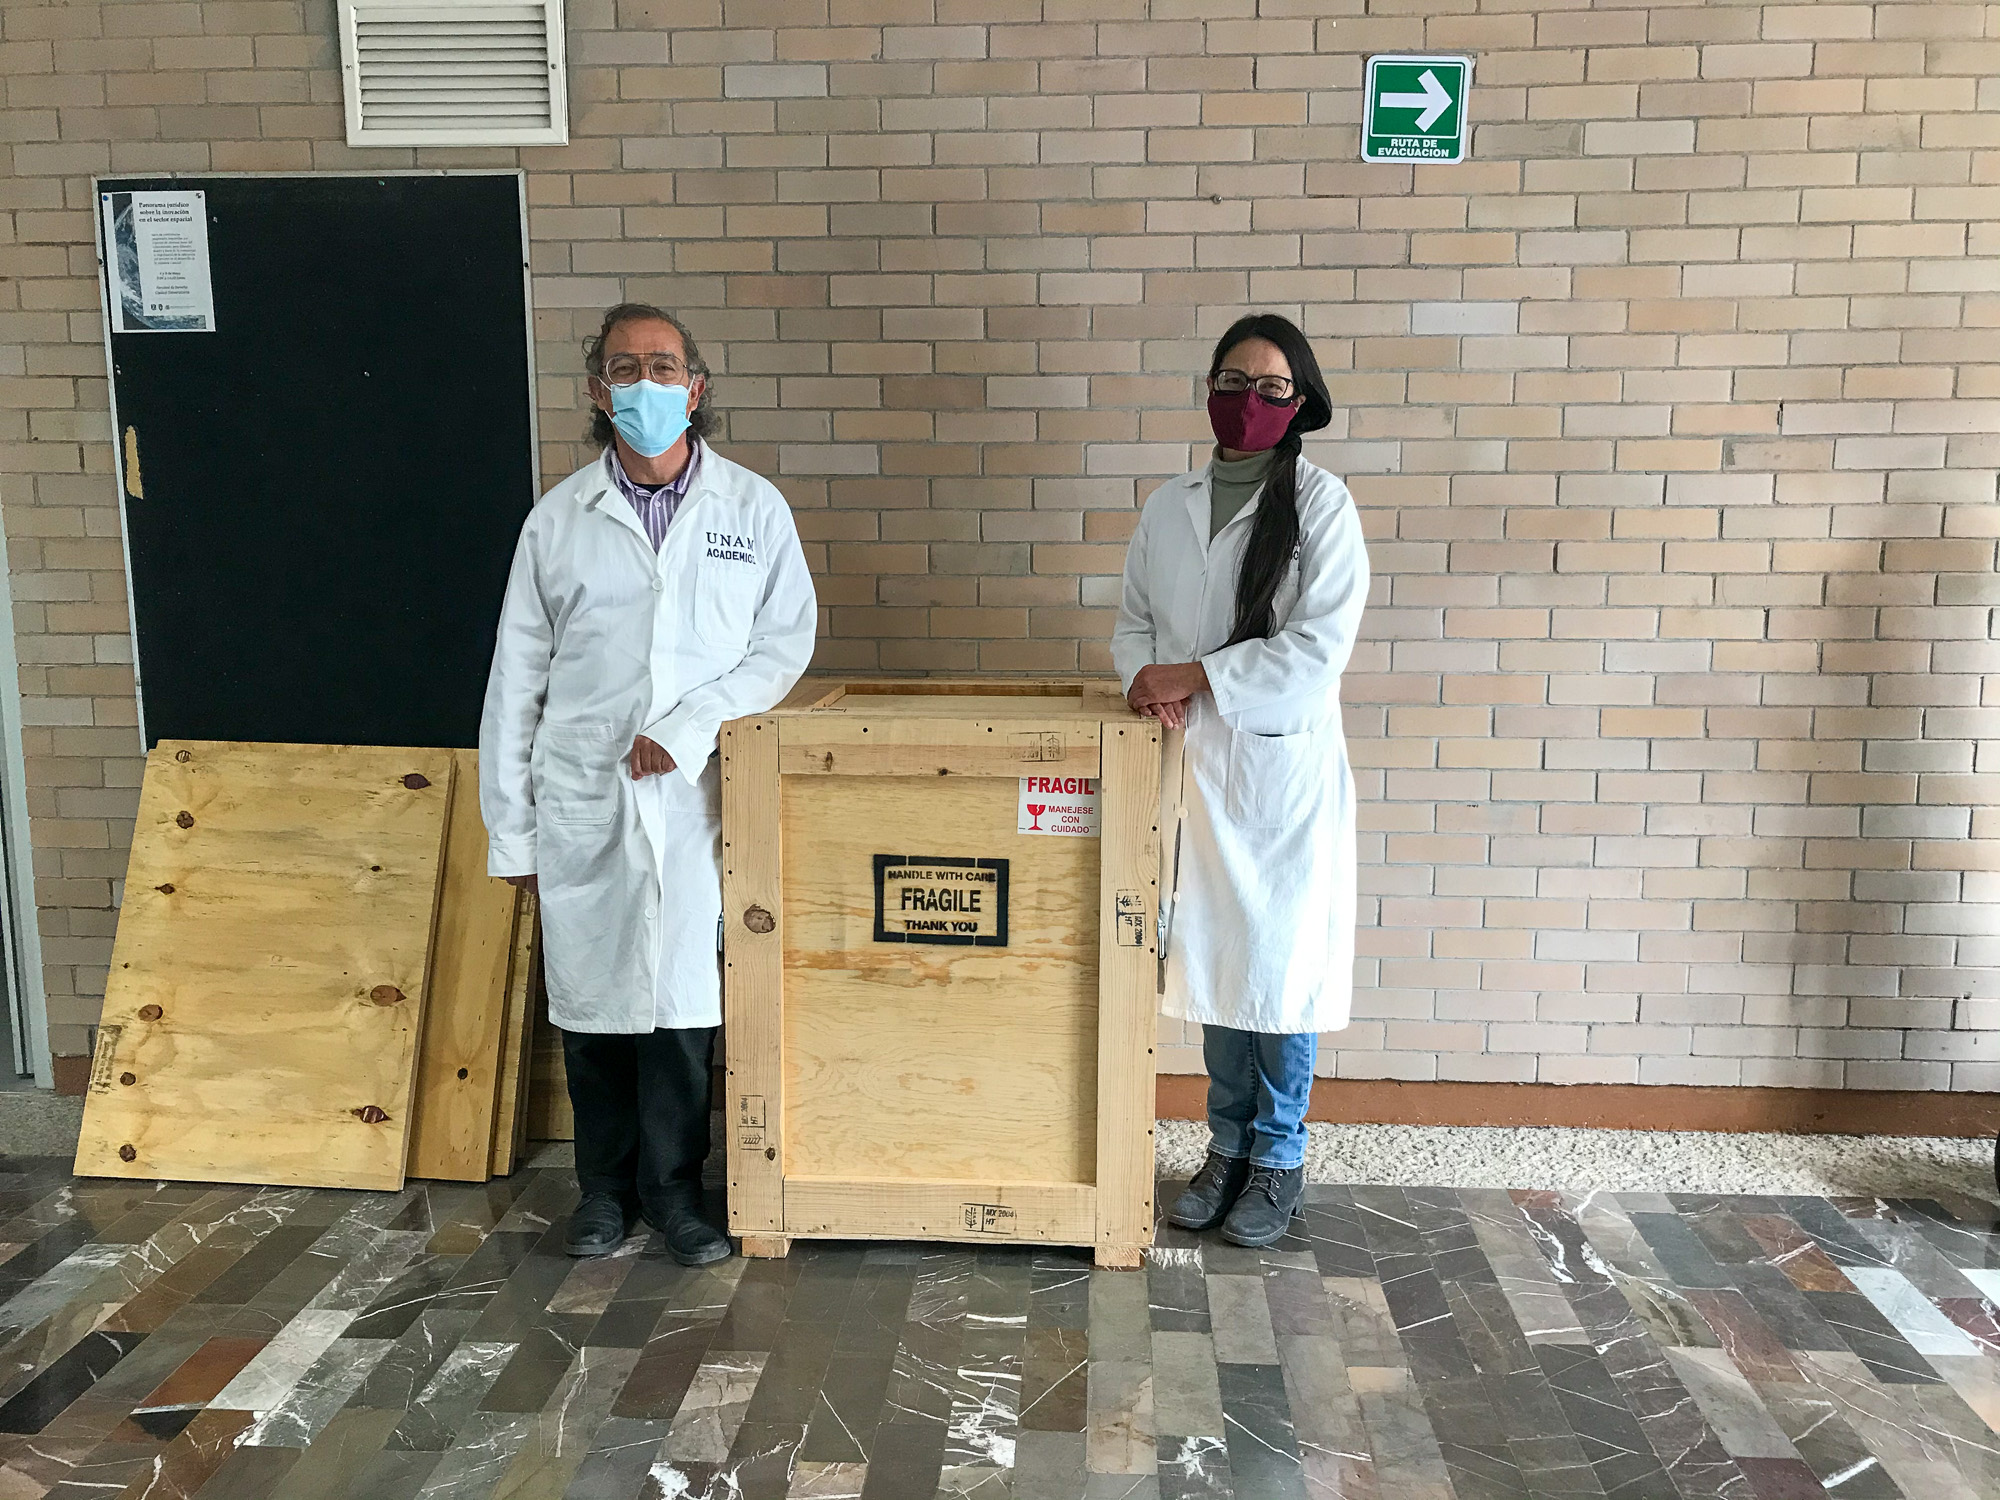
\includegraphics[width=0.60\linewidth]{figures/20201210T144505.jpg}
\end{center}
\caption{Caja 1.}
\label{figure:box-one}
\end{figure}

\begin{figure}[bp]
\begin{center}
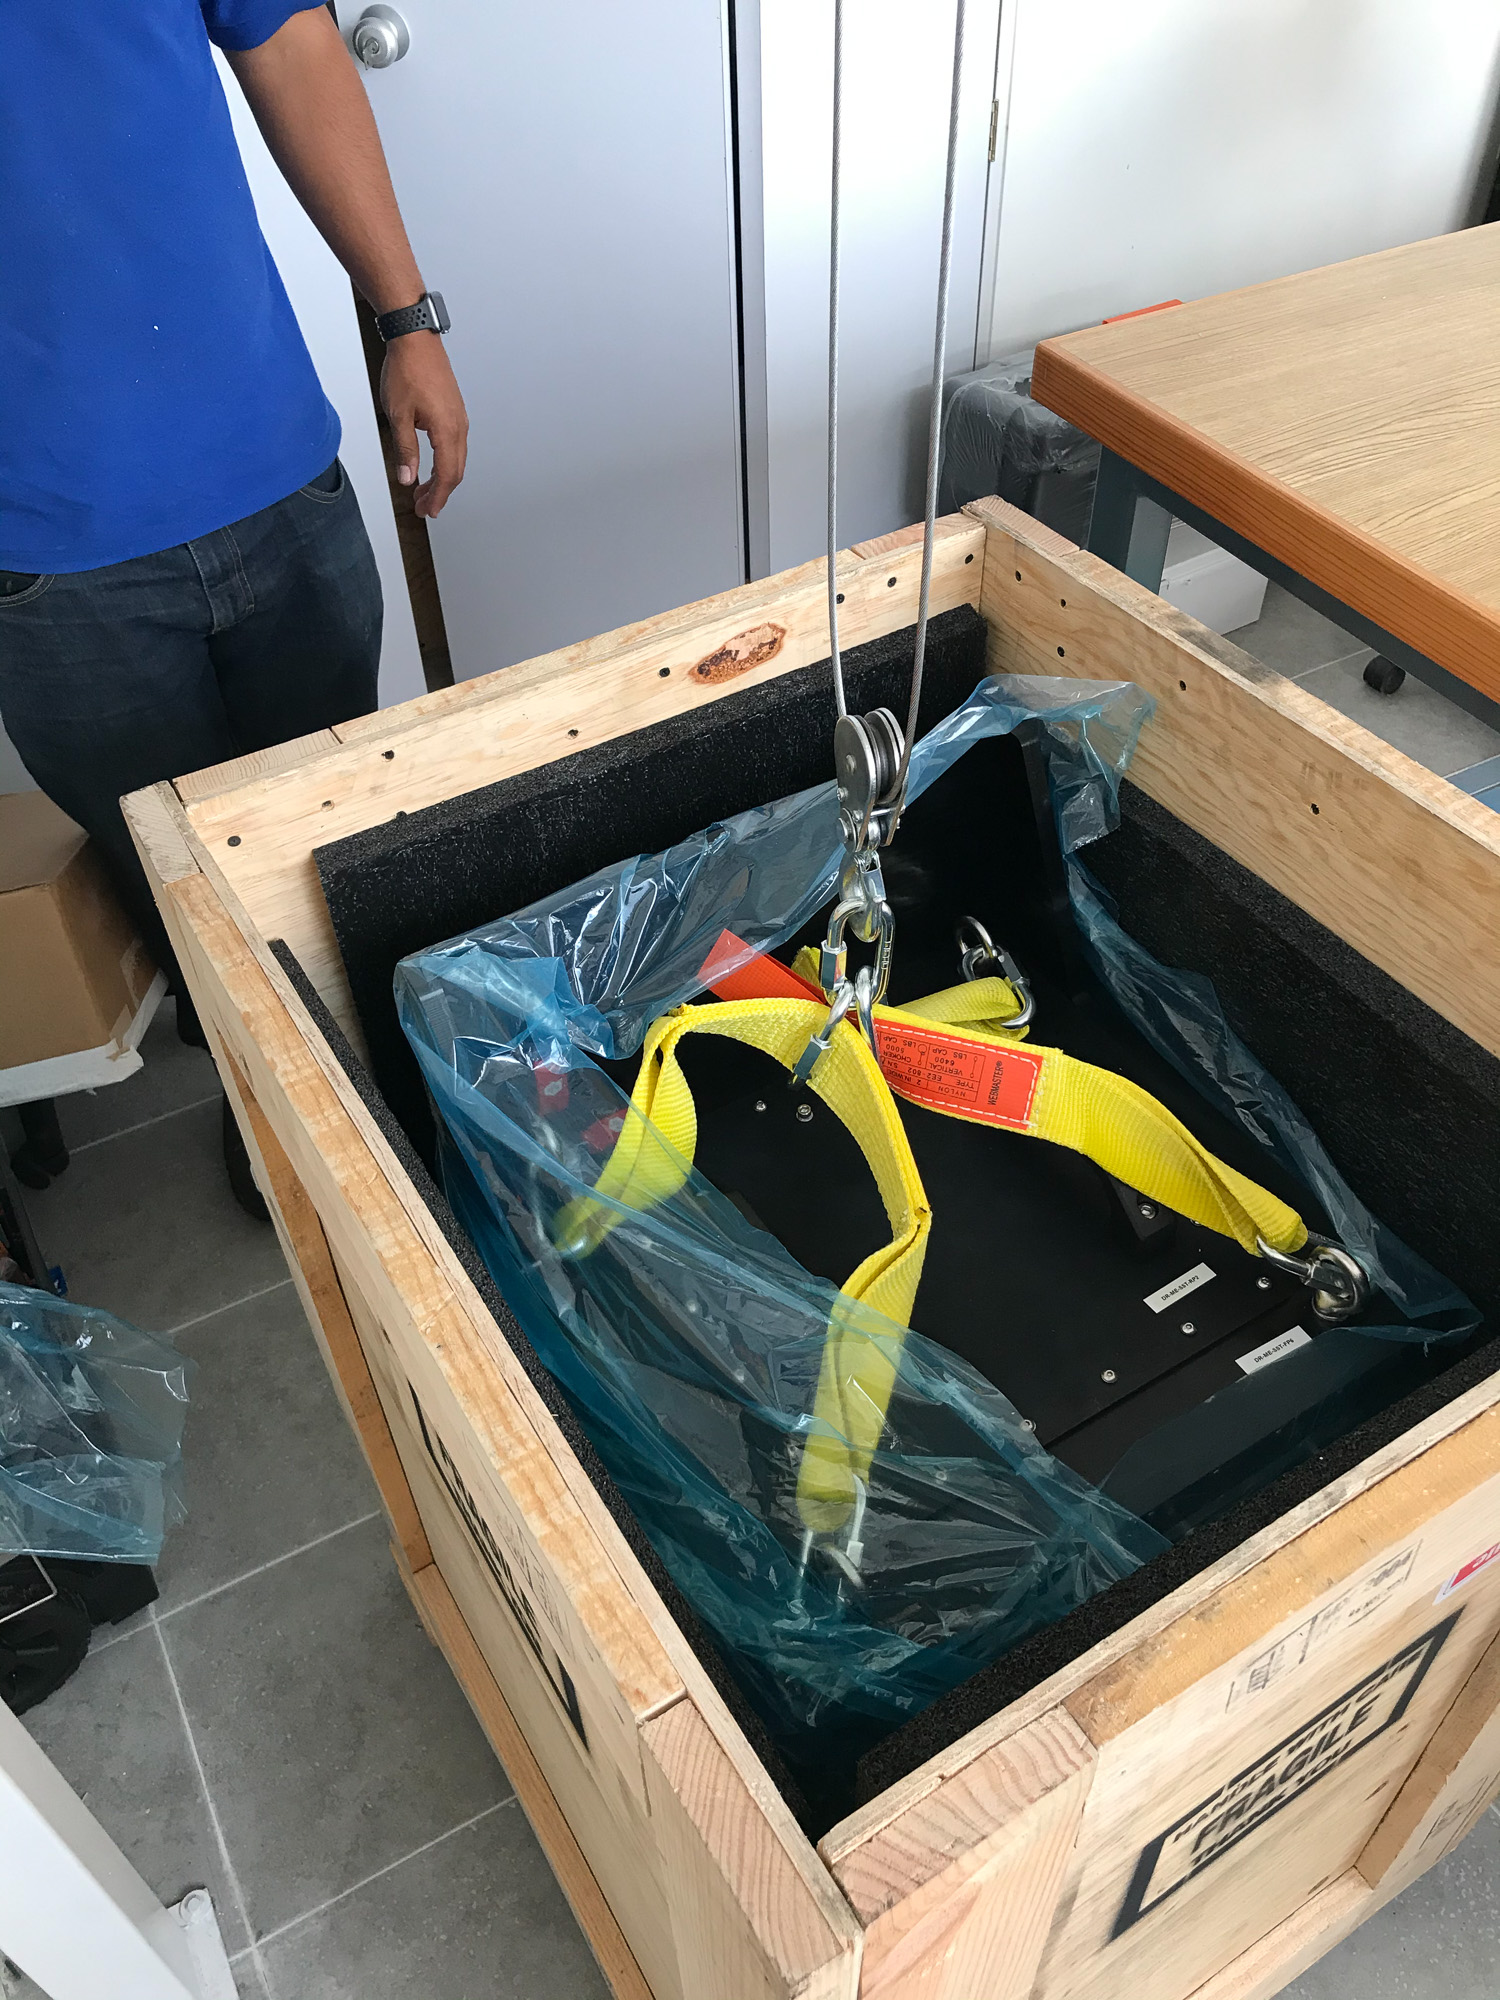
\includegraphics[width=0.3\linewidth]{figures/20201210T141602.jpg}
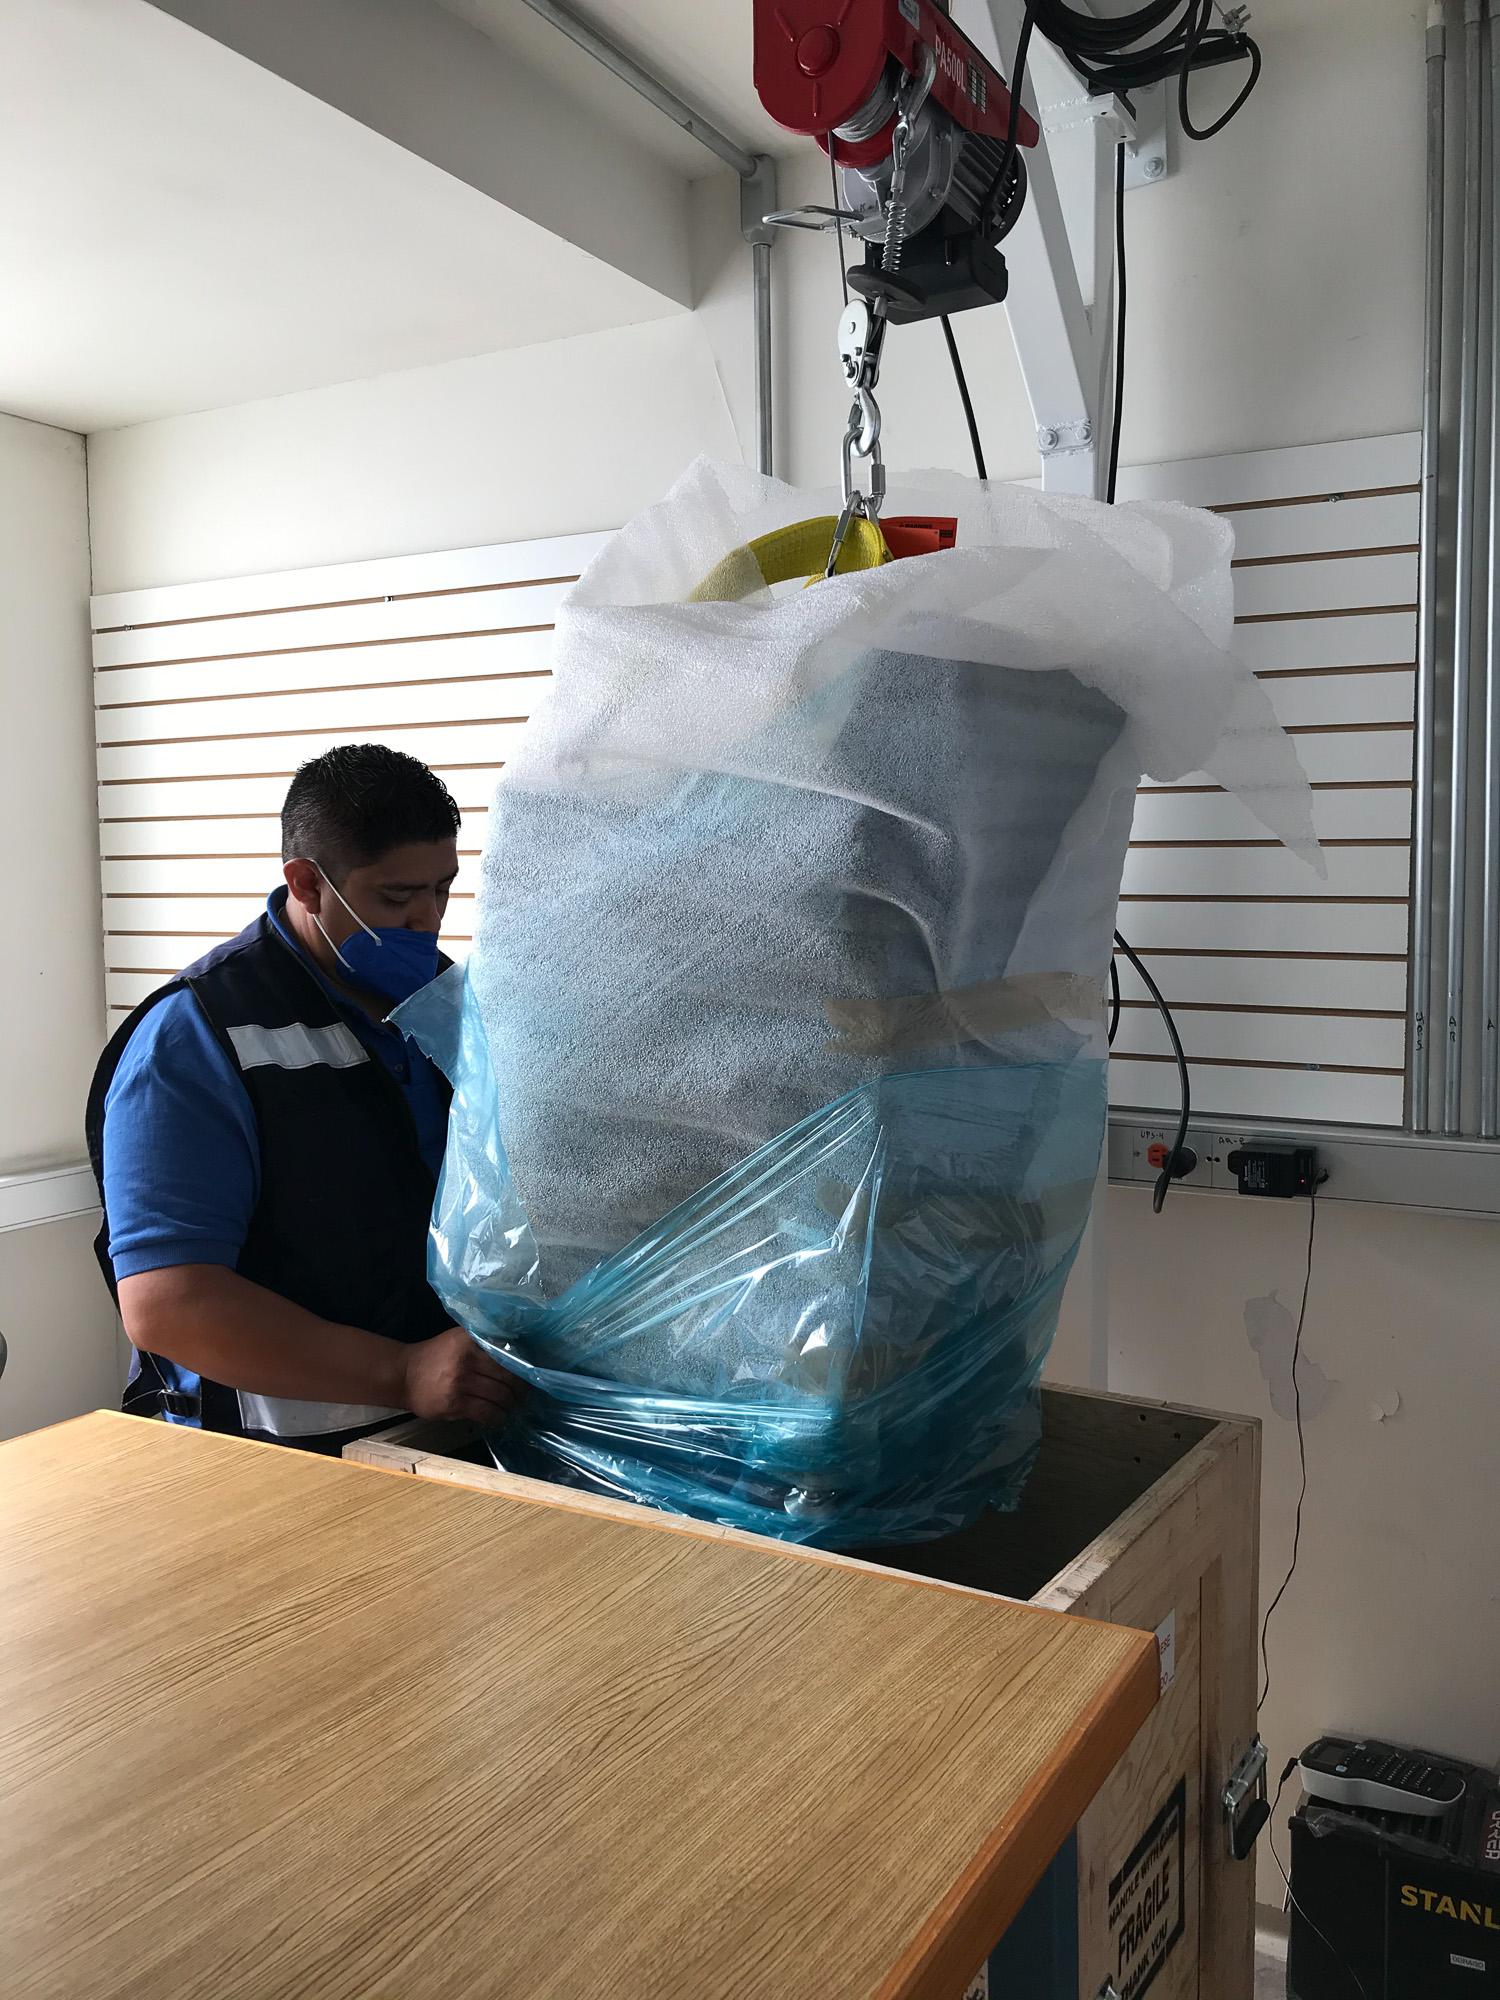
\includegraphics[width=0.3\linewidth]{figures/20201210T105541.jpg}
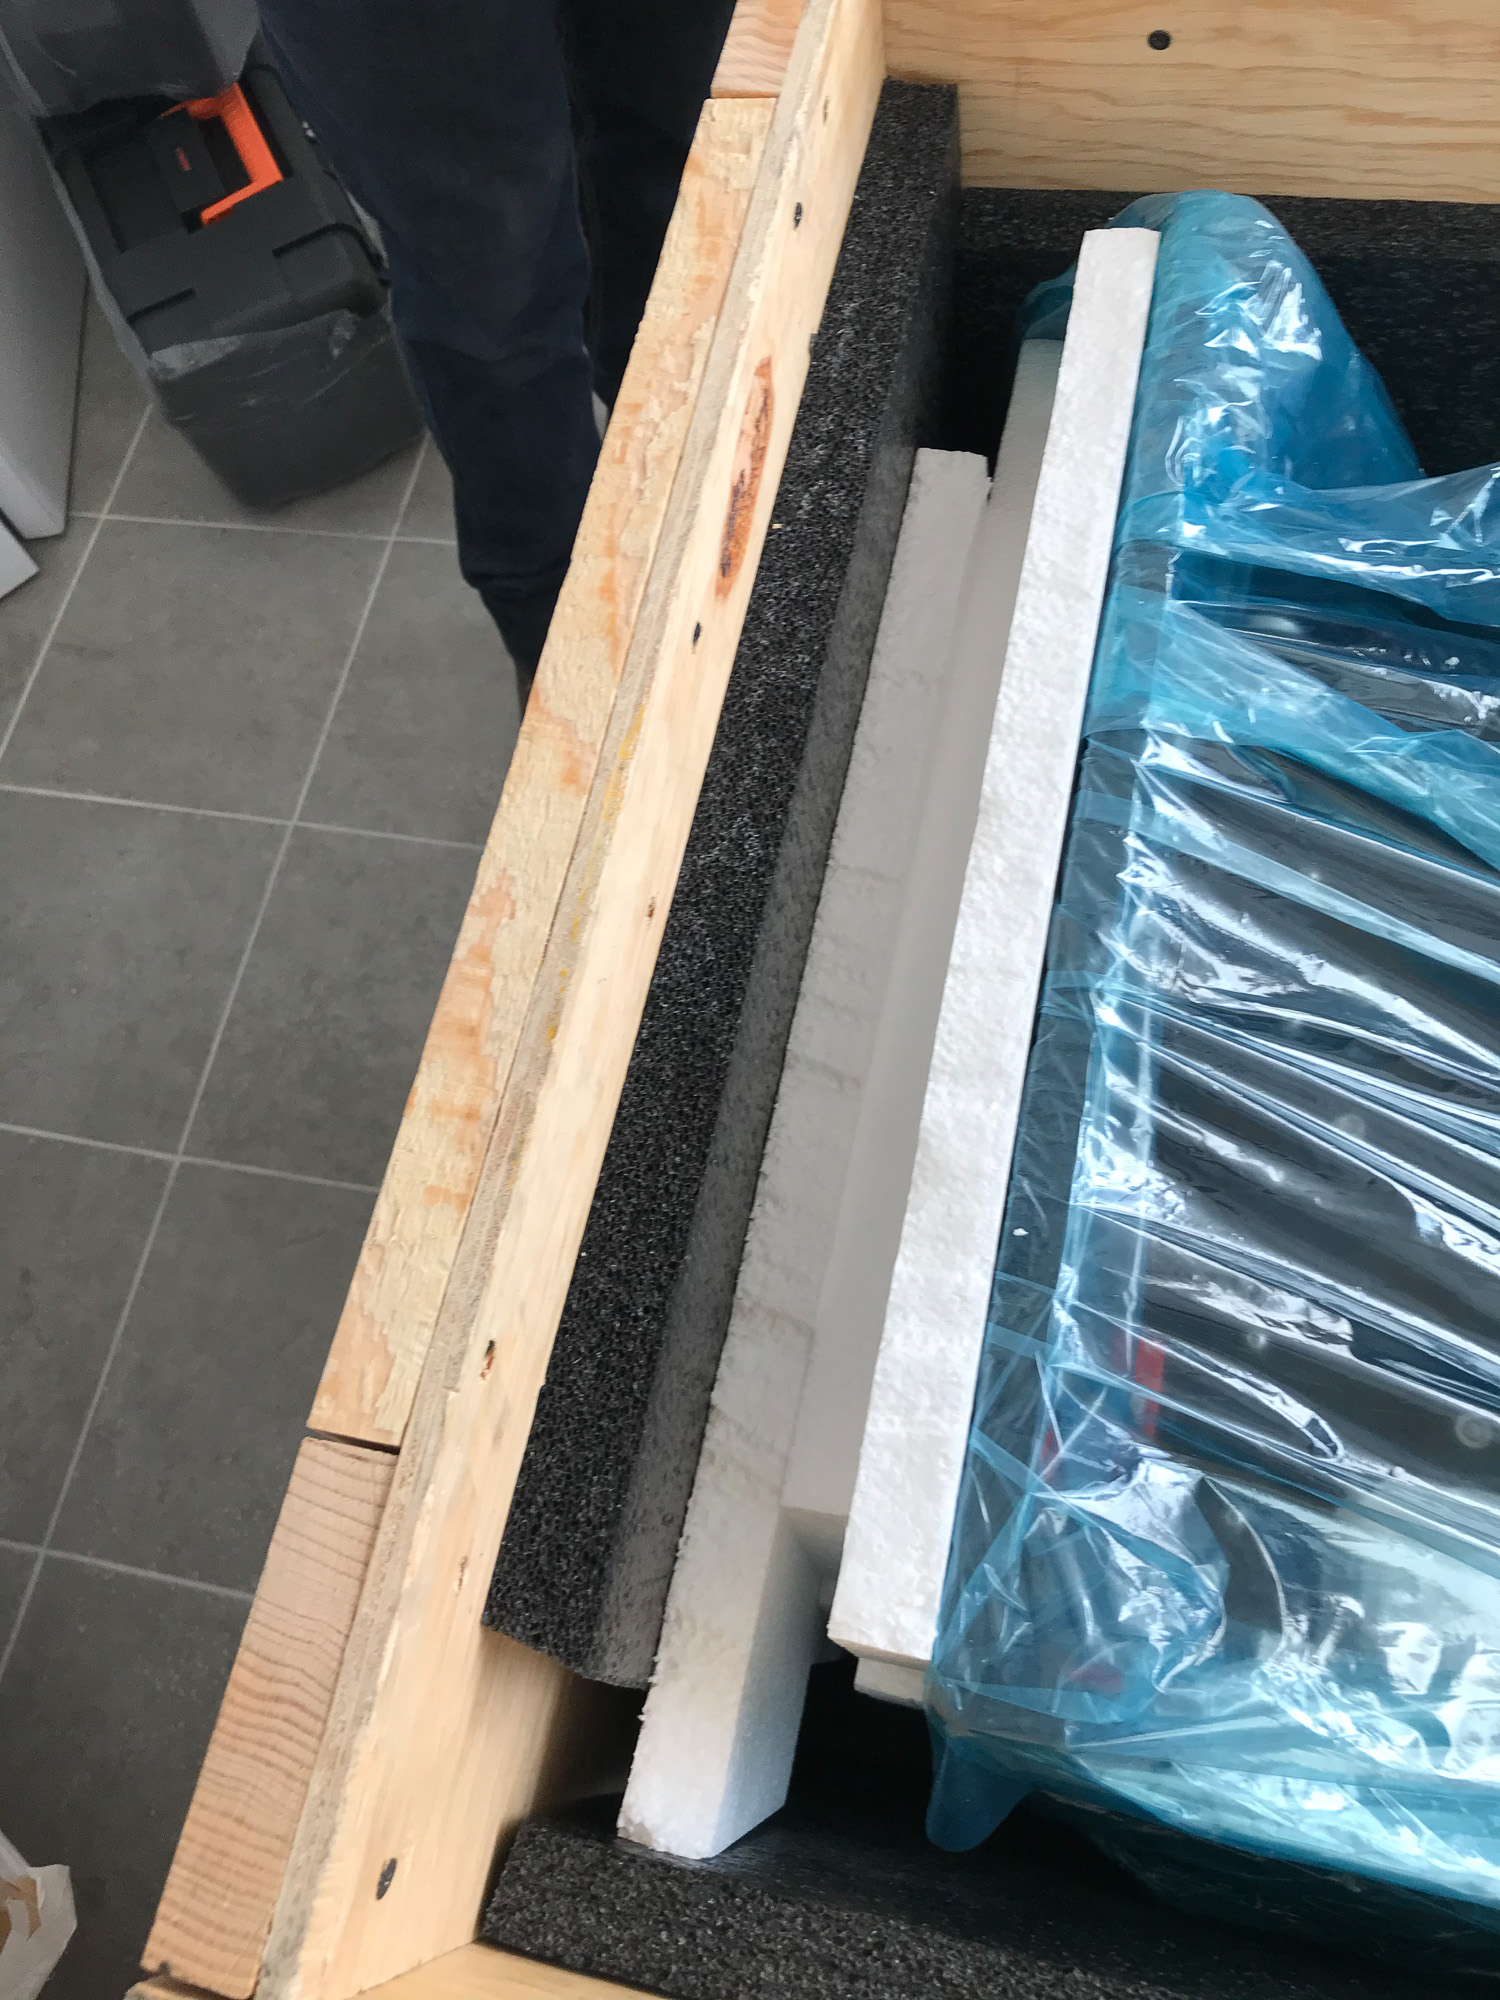
\includegraphics[width=0.3\linewidth]{figures/20201210T142939.jpg}
\end{center}
\caption{Caja 1.}
\label{figure:box-one-packing}
\end{figure}

\begin{figure}[bp]
\begin{center}
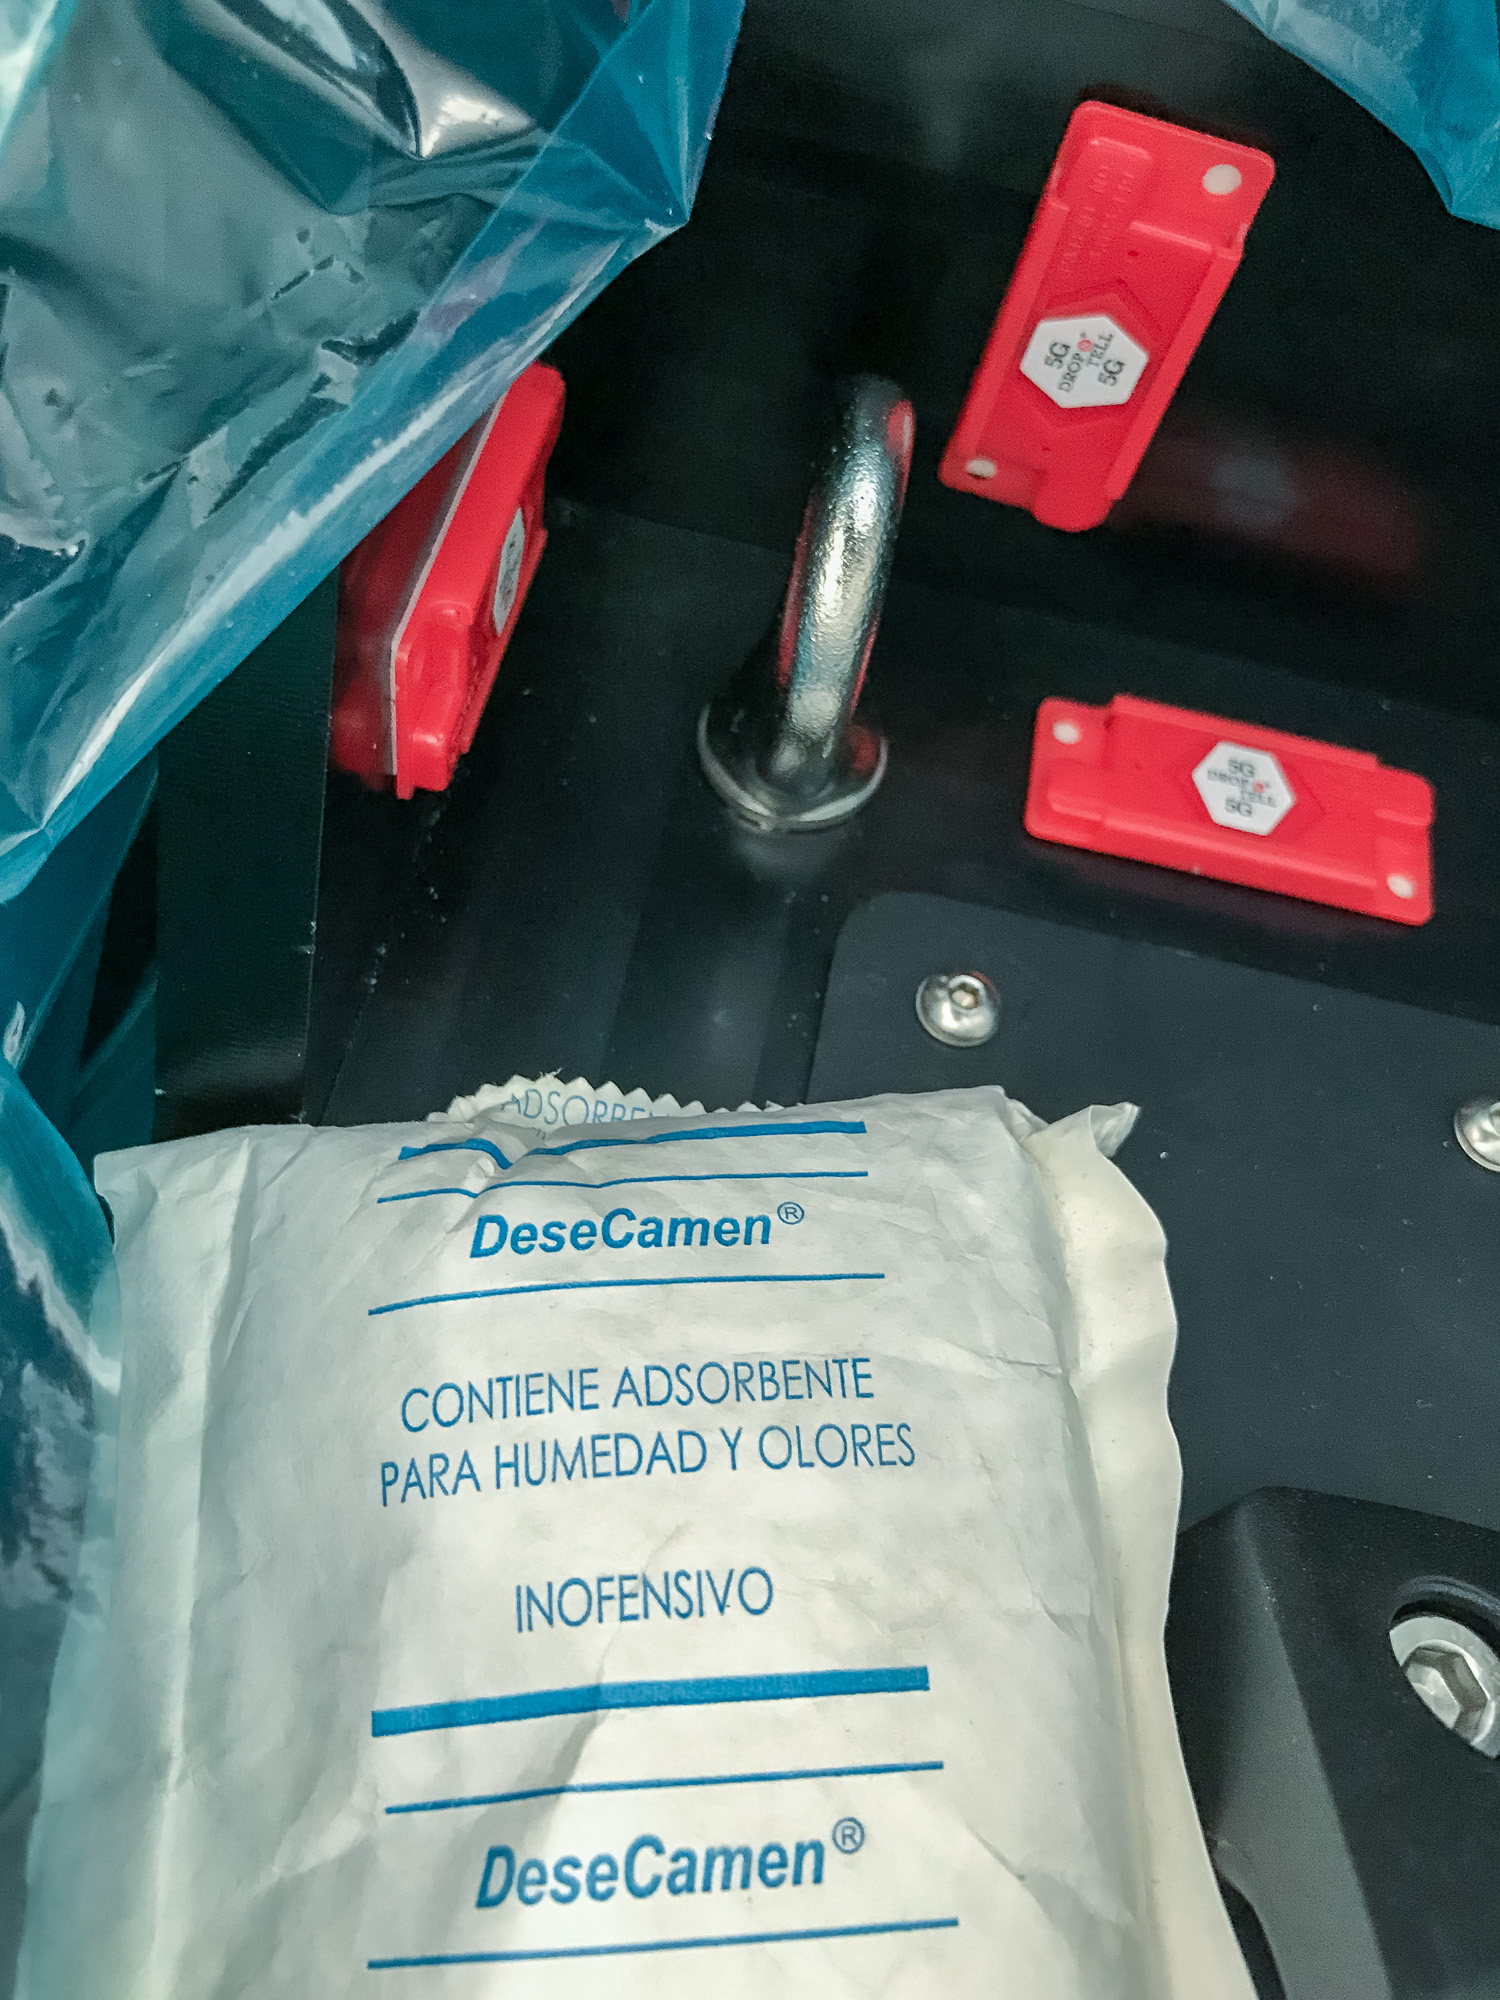
\includegraphics[width=0.3\linewidth]{figures/20210106T115707.jpg}
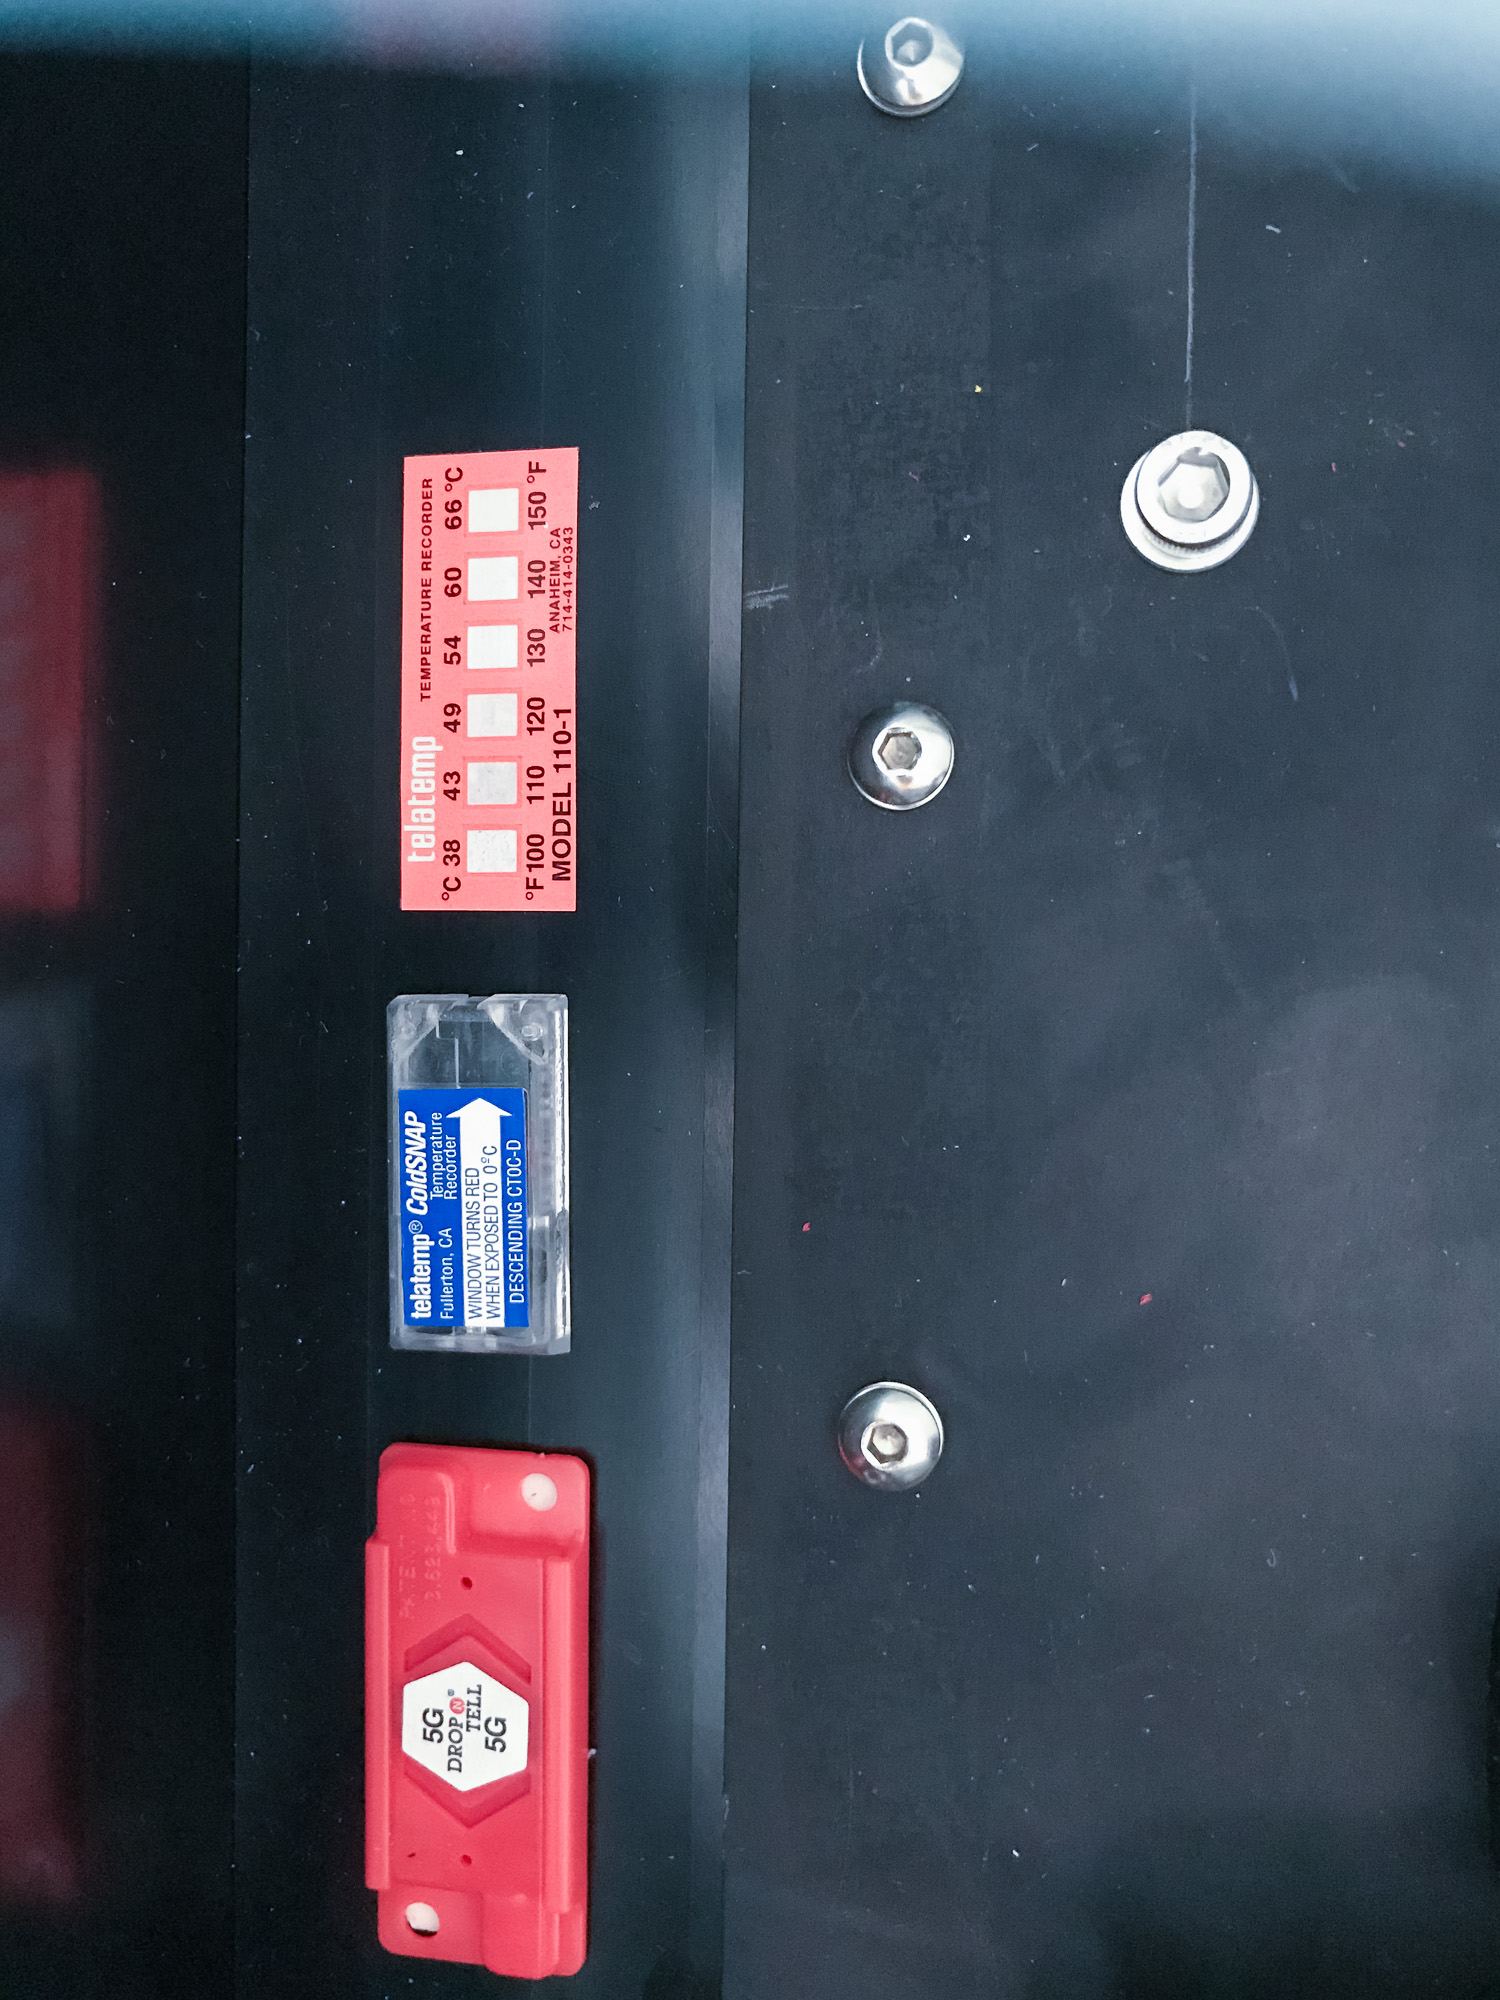
\includegraphics[width=0.3\linewidth]{figures/20210106T115933.jpg}
\end{center}
\caption{Box 1 internal sensors on the top of the instrument. Left: the three 5$g$ sensors. Right: the temperature sensors.}
\label{figure:box-one-internal-sensors}
\end{figure}

\begin{figure}[bp]
\begin{center}
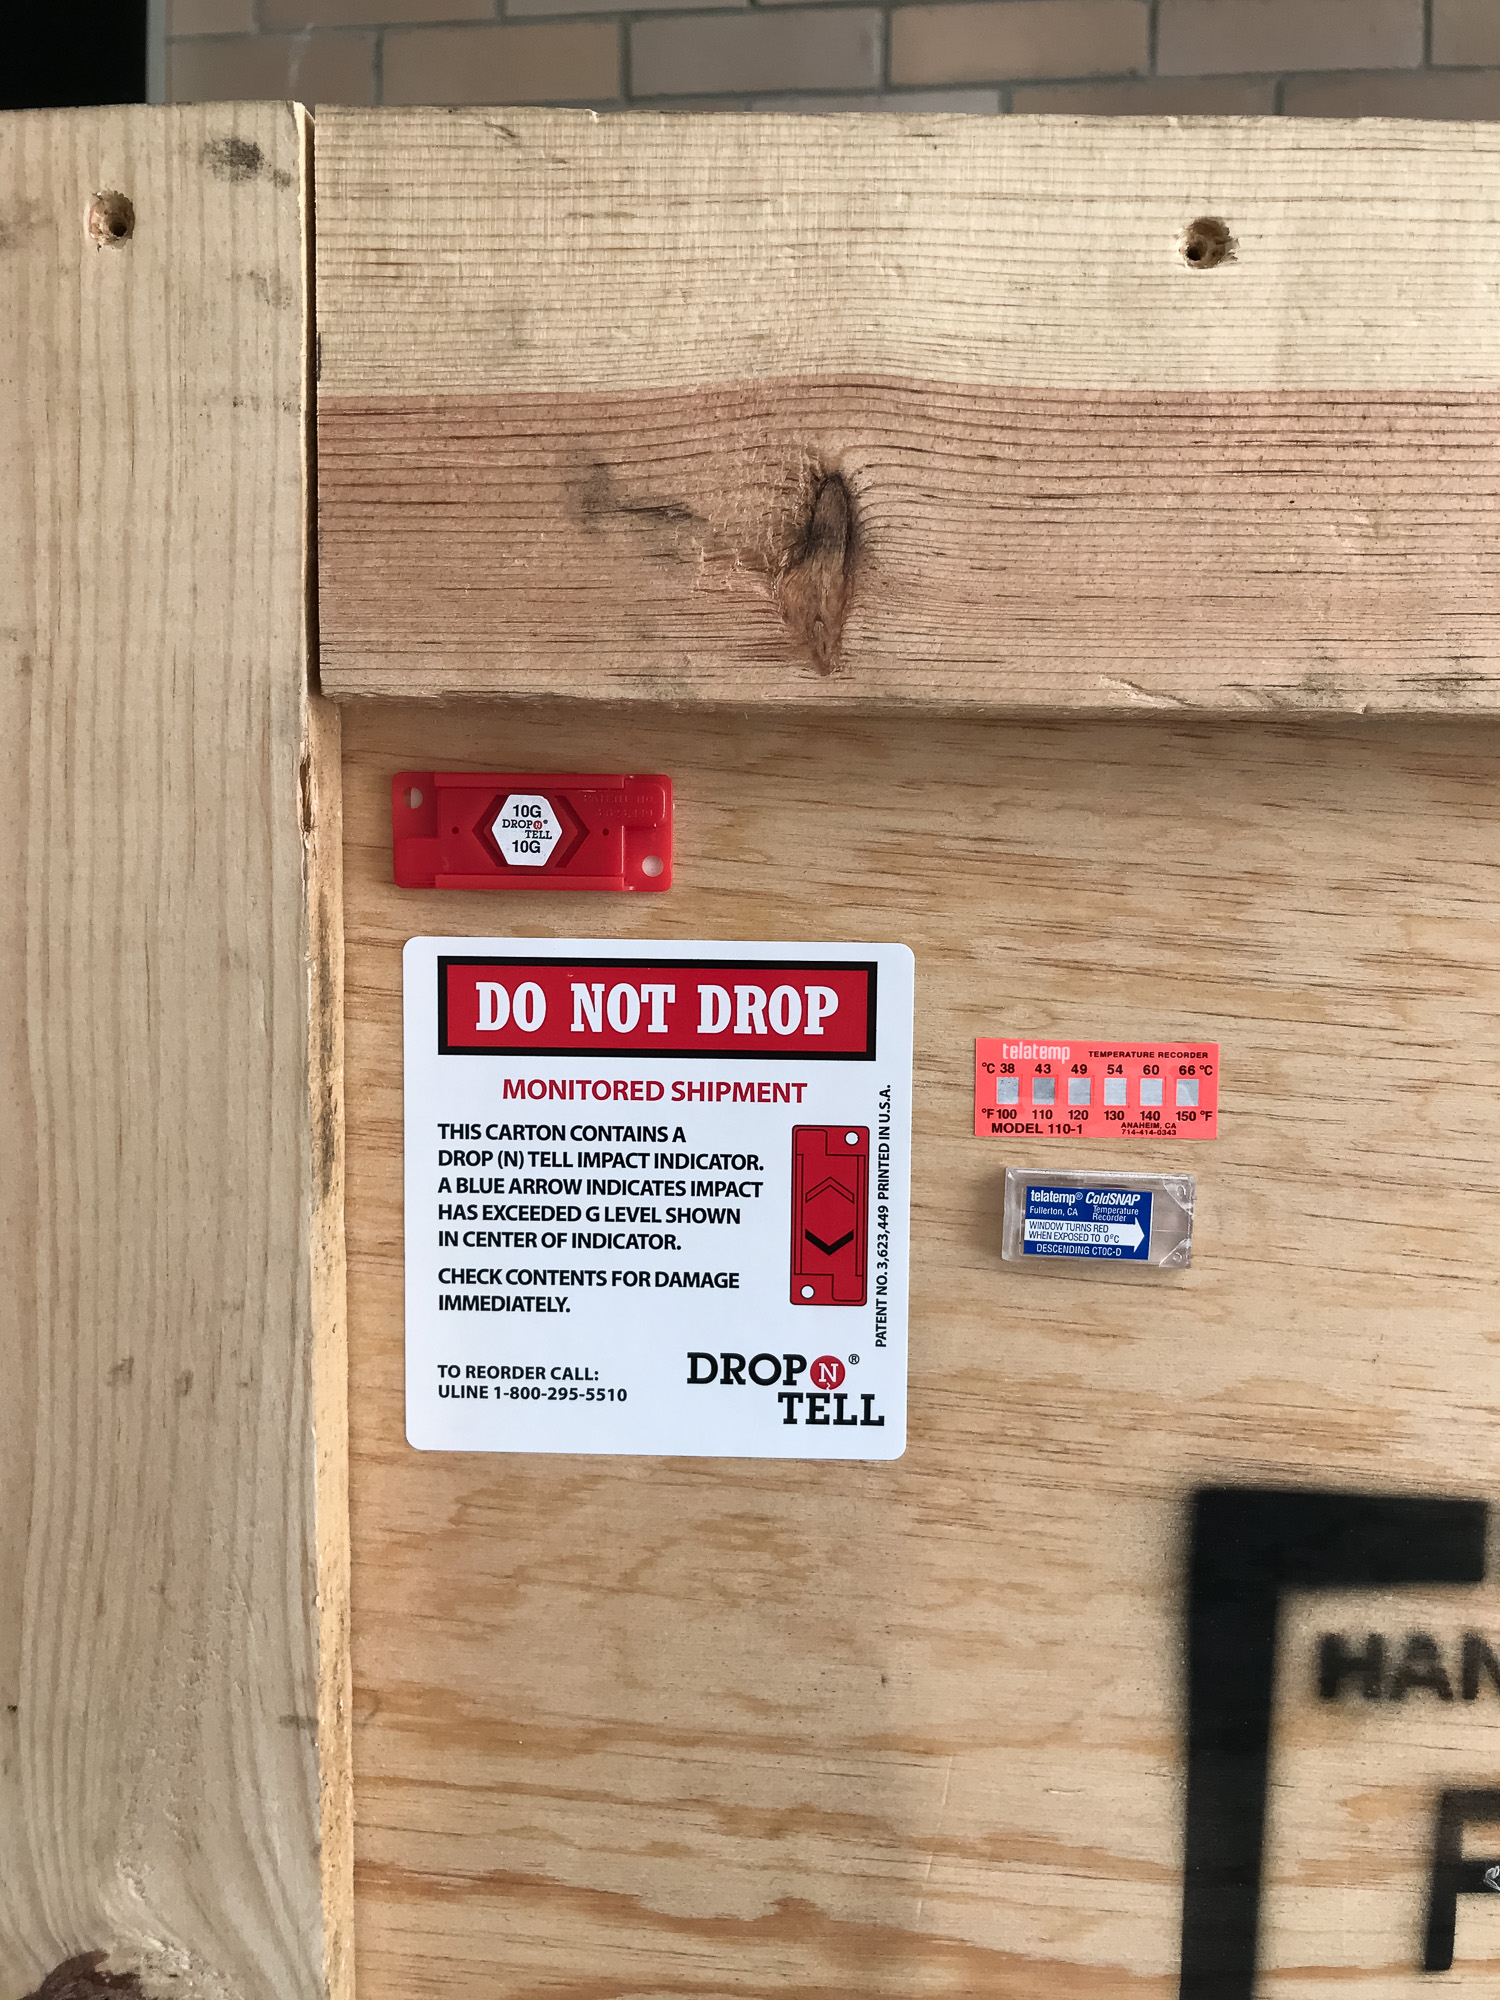
\includegraphics[width=0.3\linewidth]{figures/20210106T120242.jpg}
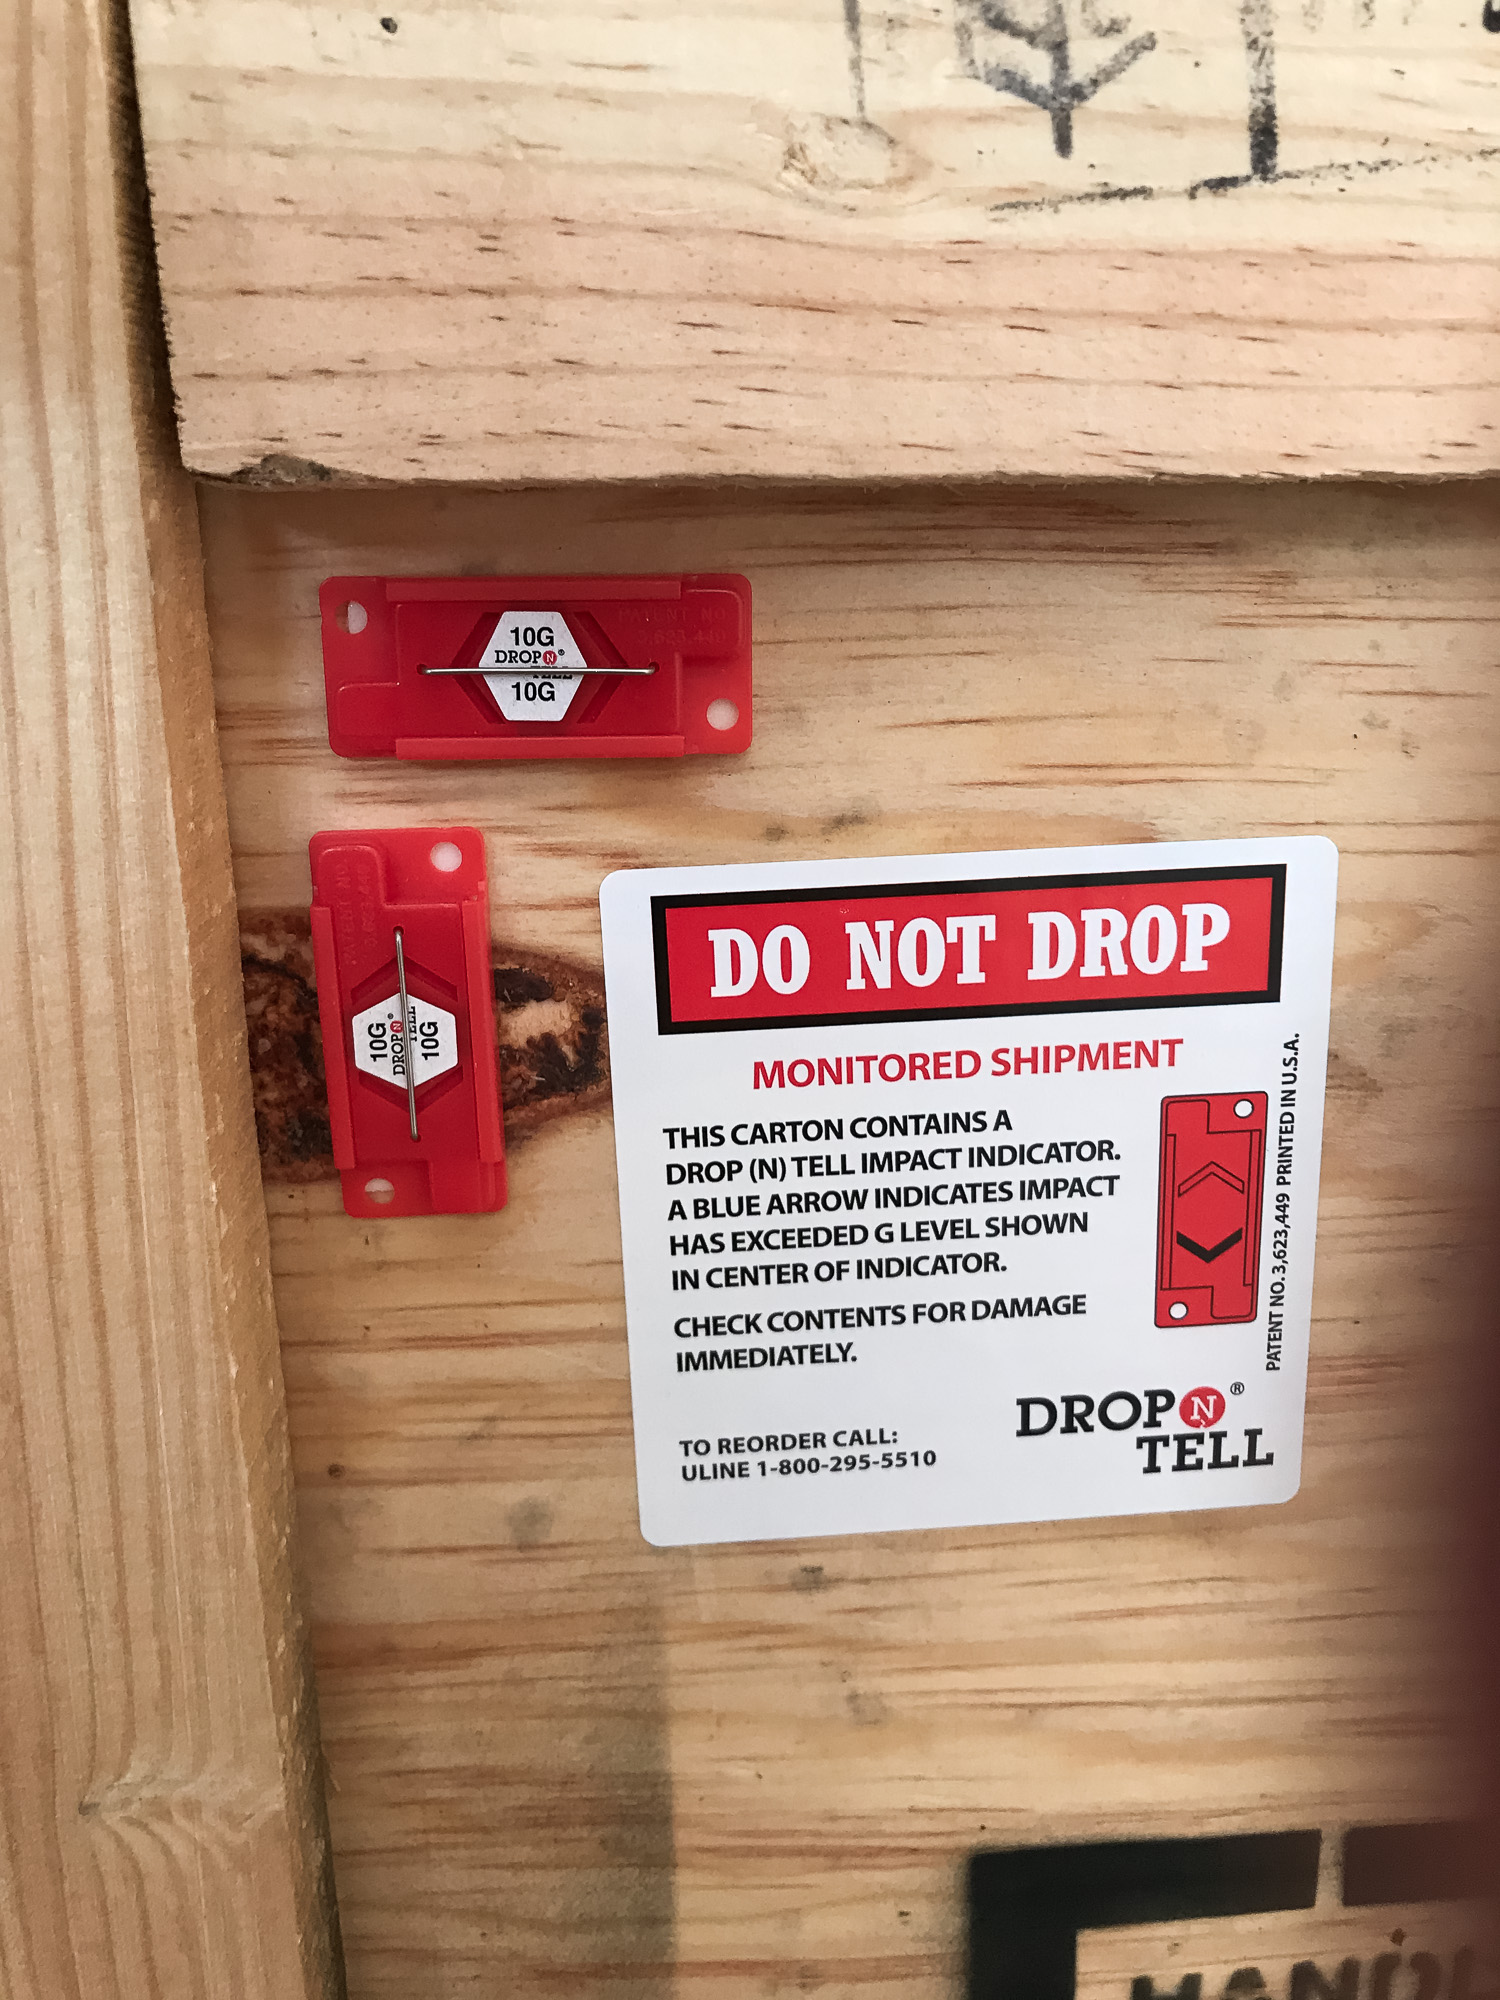
\includegraphics[width=0.3\linewidth]{figures/20210106T113233.jpg}
\end{center}
\caption{Box 1 external sensors. Left: one of the three 10$g$ sensors and the temperature sensors. Right: the other two 10$g$ sensors.}
\label{figure:box-one-external-sensors}
\end{figure}

\subsection{Description}

Box 1 contains:

\begin{itemize}
    \item The main instrument structure.
\end{itemize}

See Figure~\ref{figure:box-one}.

The box is a custom-made wooden crate and is lined with foam. There are three 10-g impact indicators and temperature sensors on the outside of the box (see Figure~\ref{figure:box-one-external-sensors}) and three 5-g indicators and temperature sensors inside the box on the upper section of the main structure (se Figure~\ref{figure:box-one-internal-sensors}).

Box 1 is $75 \times 67 \times 97$ cm ($L \times W \times H$) and has a weight of 110 kg.

\subsection{Unpacking Instructions}

\begin{enumerate}
\item Verify that the external 10-g impact indicators are not activated. If they are, consult with the UNAM team before proceeding further.
\item Verify that the external temperature sensors are not activated. If they are, consult with the UNAM team before proceeding further.
\item Remove the 16 screws that fasten the lid of the box. Remove the lid.
\item Verify that the internal 5-g impact indicators are not activated. If they are, consult with the UNAM team before proceeding further.
\item Verify that the internal temperature sensors are not activated. If they are, consult with the UNAM team before proceeding further.
\item Remove the foam sheets between the front of the instrument and the box. See Figure~\ref{figure:box-one-packing}.
\item Connect a harness to the lifting eye-bolts  (DR-ME-SST-LEB). In Mexico, we used two two slings (DR-ME-MH-SL) and 
five connecting links (DR-ME-MH-CL). See Figure~\ref{figure:box-one-packing}.
\item Lift the support structure using a crane. Remove the box. Lower the support structure.
\item Remove the harness.
\item Fasten the lid in place with 16 screws.
\end{enumerate}

\subsection{Repacking Instructions}

\begin{enumerate}
\item Verify that the external 10-g and internal 5-g impact indicators are not activated. If they are, replace them with spares from Box 28.
\item Verify that the external and internal temperature sensors are not activated. If they are, replace them with spares from Box 28.
\item Connect a harness to the lifting eye-bolts  (DR-ME-SST-LEB). In Mexico, we used two two slings (DR-ME-MH-SL) and 
five connecting links (DR-ME-MH-CL). See Figure~\ref{figure:box-one-packing}.
\item Lift the instrument.
\item Wrap the instrument in foam and plastic sheet.
\item Lower the instrument into the box.
\item Remove the harness.
\item Pack the space between the front of the instrument and the box with foam sheets. The aim here is that the force of impacts are not transfered to the L1L2 barrel.
\item Add desiccant.
\item Fasten the lid in place with 16 screws.
\end{enumerate}

%%%%%%%%%%%%%%%%%%%%%%%%%%%%%%%%%%%%%%%%%

\clearpage
\section{Box 2}

\begin{figure}[bp]
\begin{center}
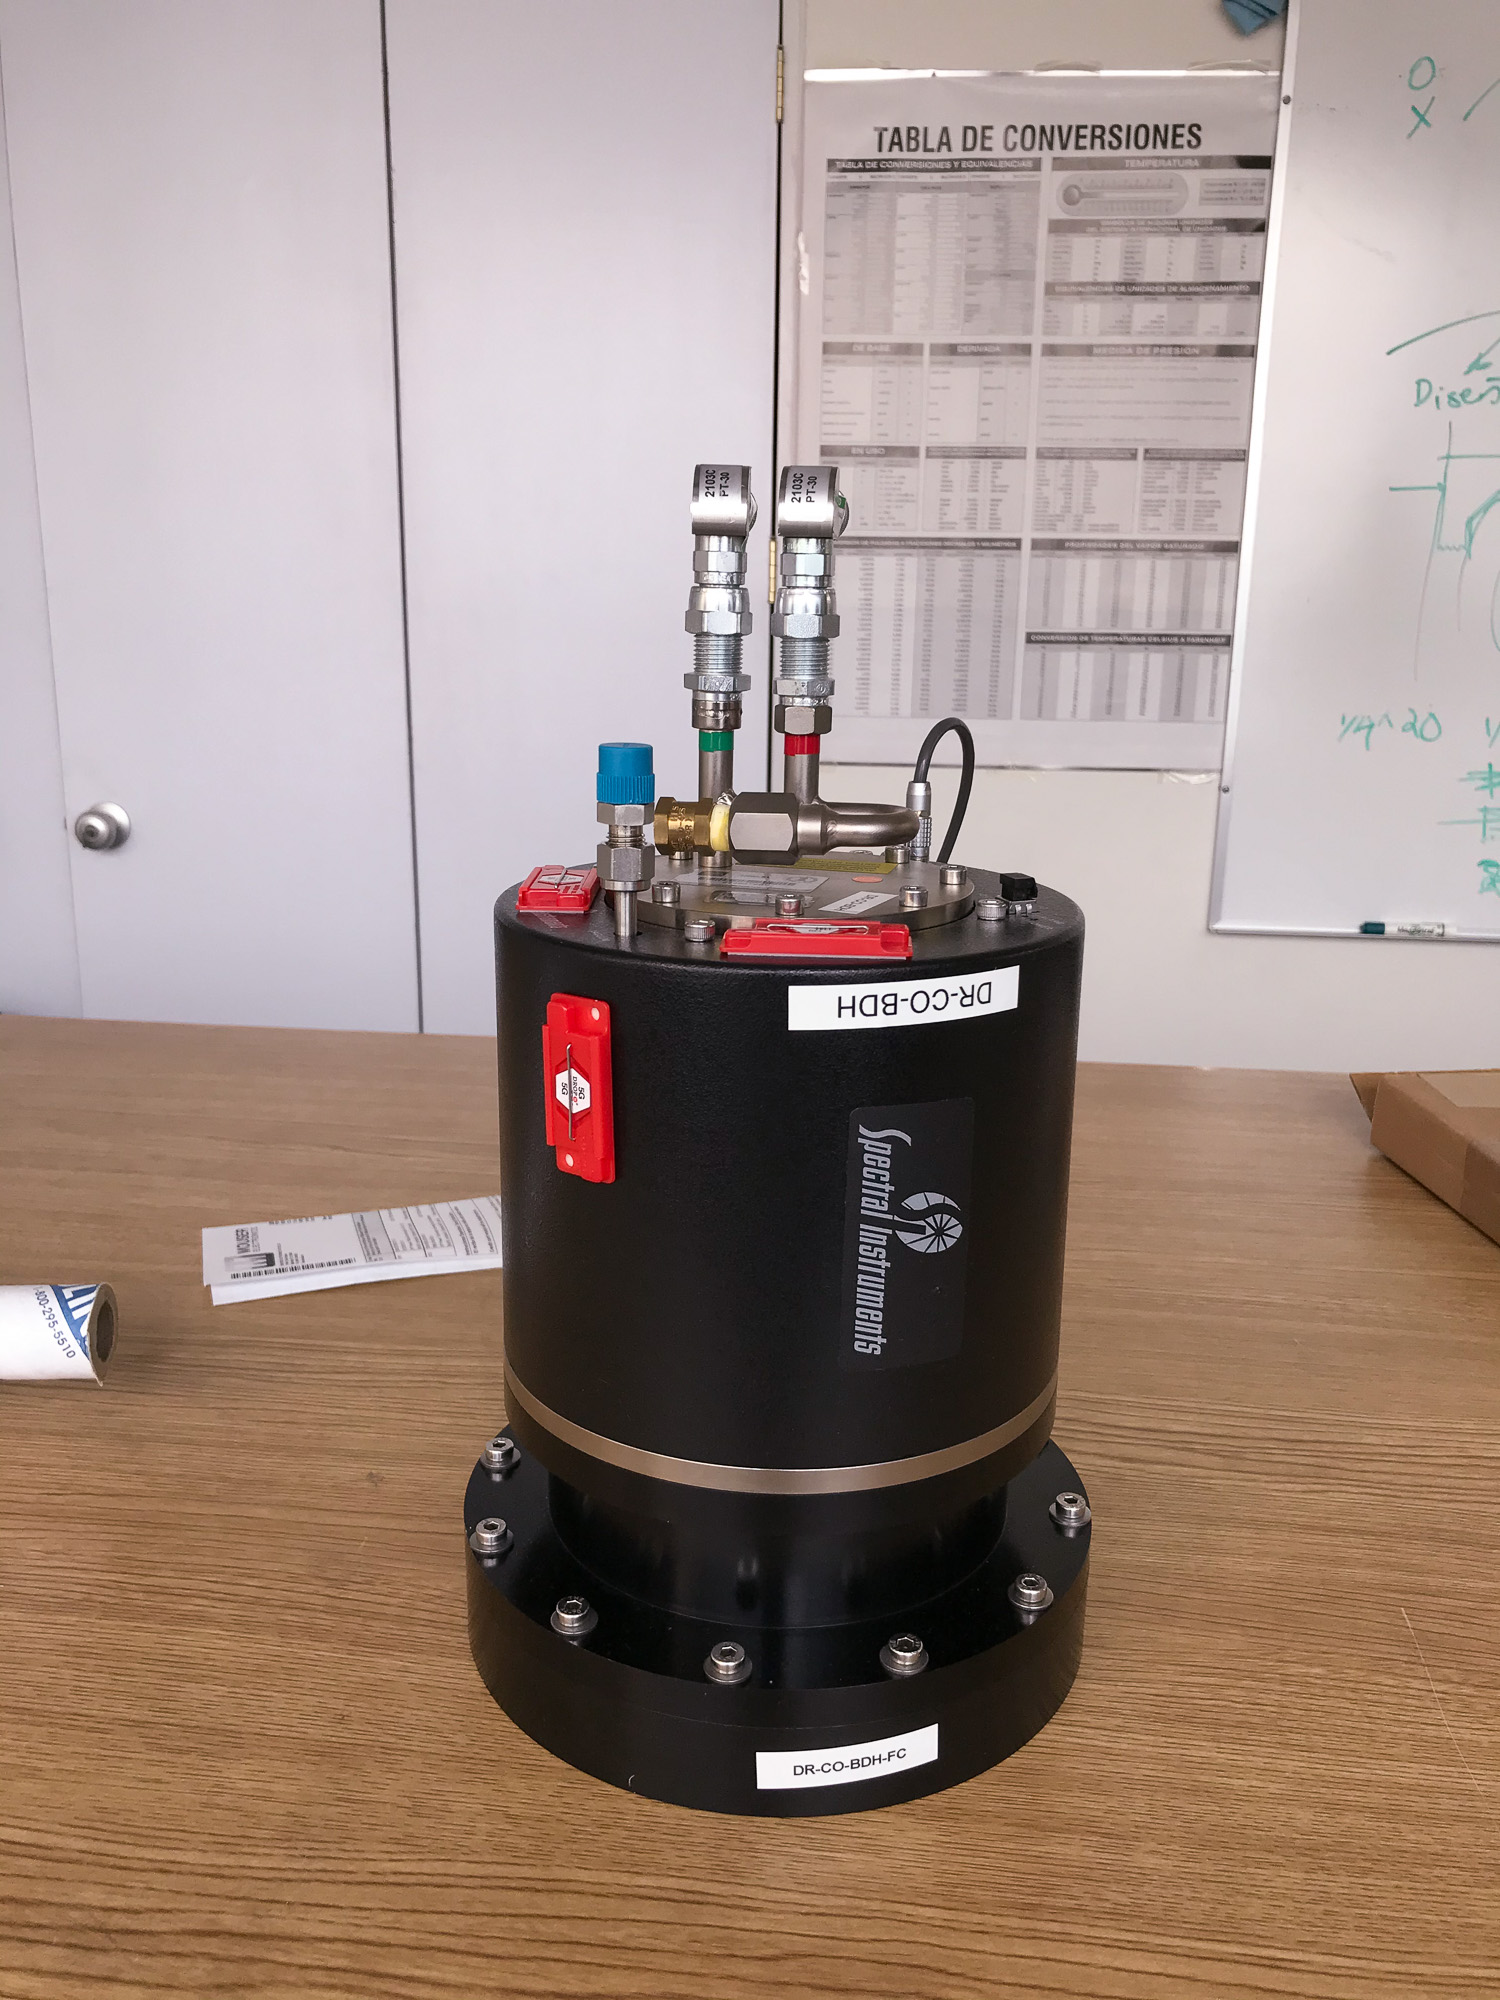
\includegraphics[width=0.30\linewidth]{figures/20201210T100146.jpg}
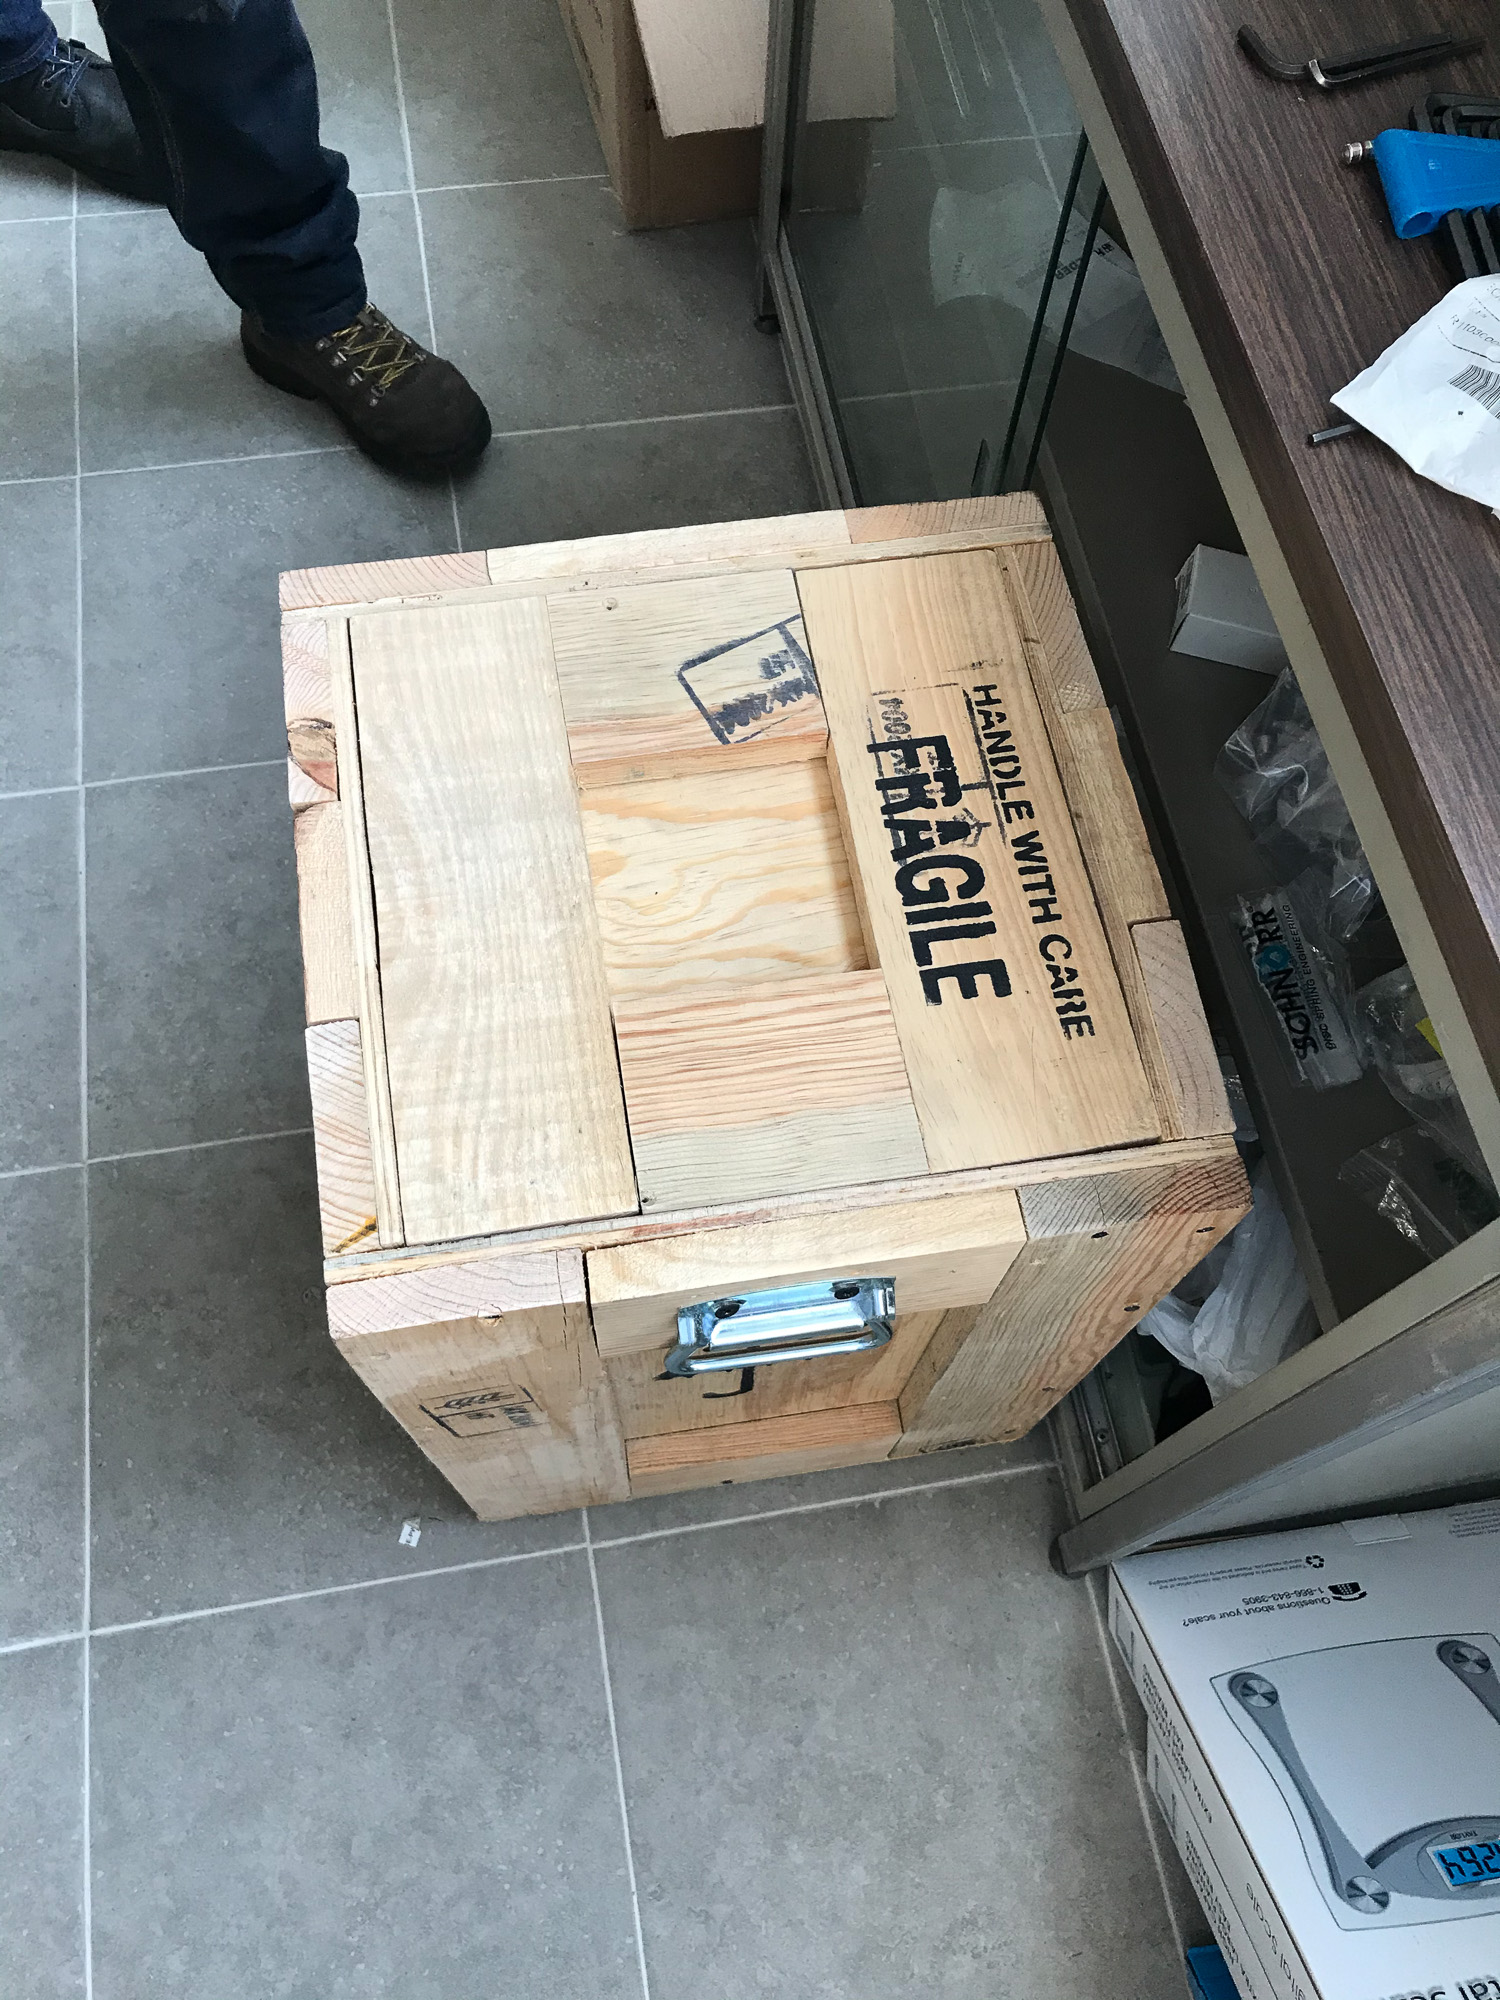
\includegraphics[width=0.30\linewidth]{figures/20201210T101147.jpg}\\
\end{center}
\caption{Box 2 and its contents.}
\label{figure:box-two}
\end{figure}

\begin{figure}[bp]
\begin{center}
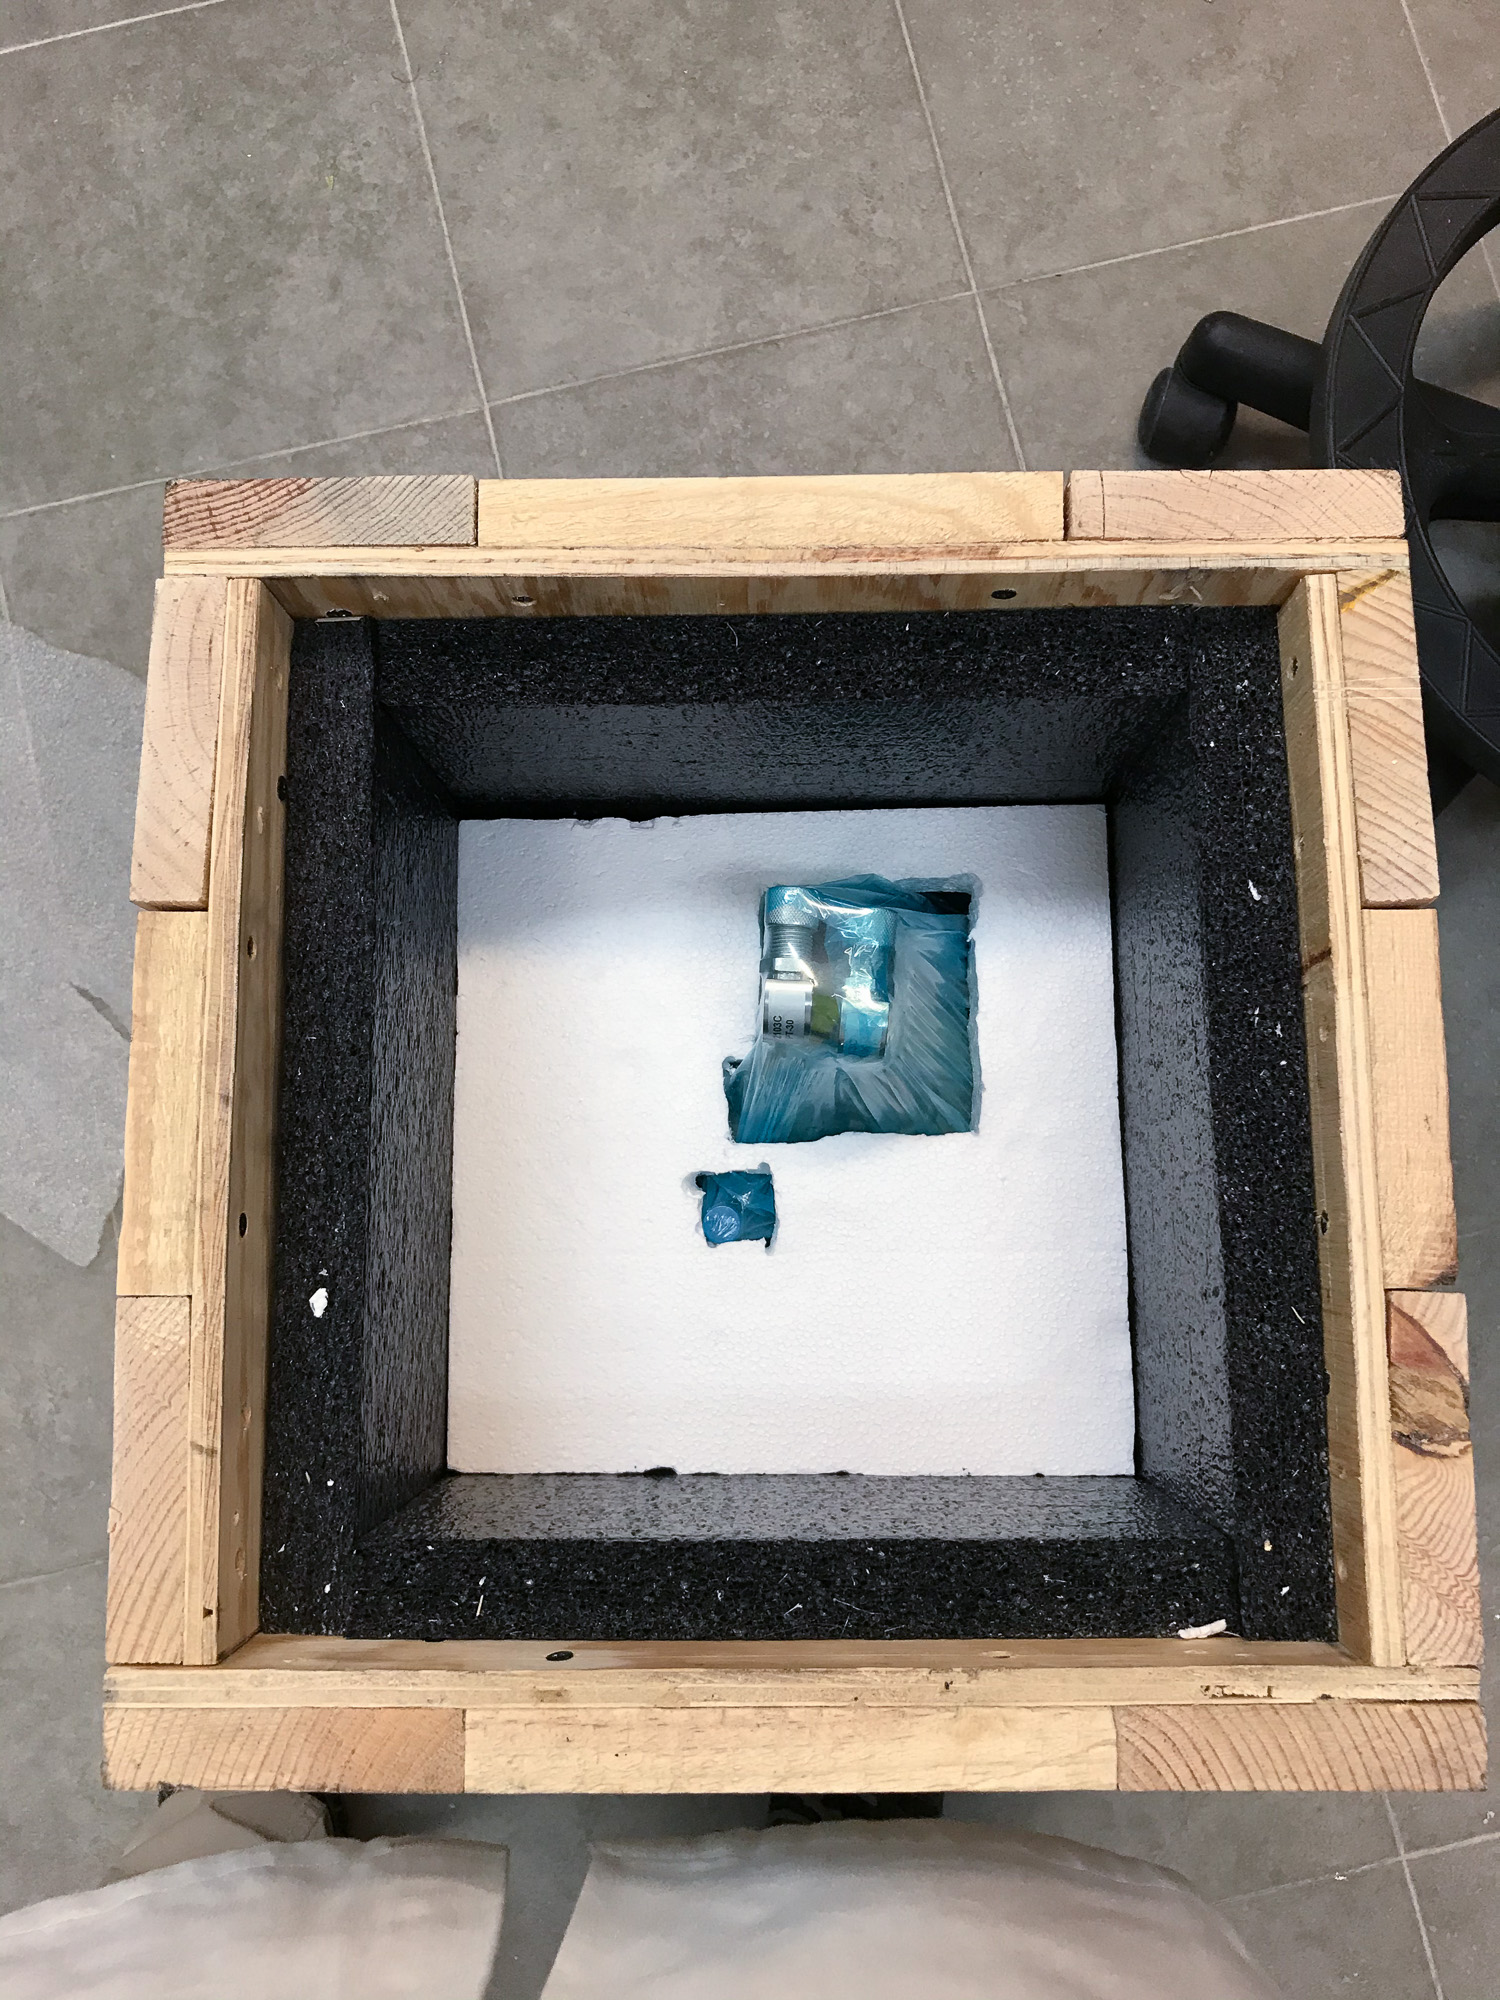
\includegraphics[width=0.30\linewidth]{figures/20201210T114228.jpg}
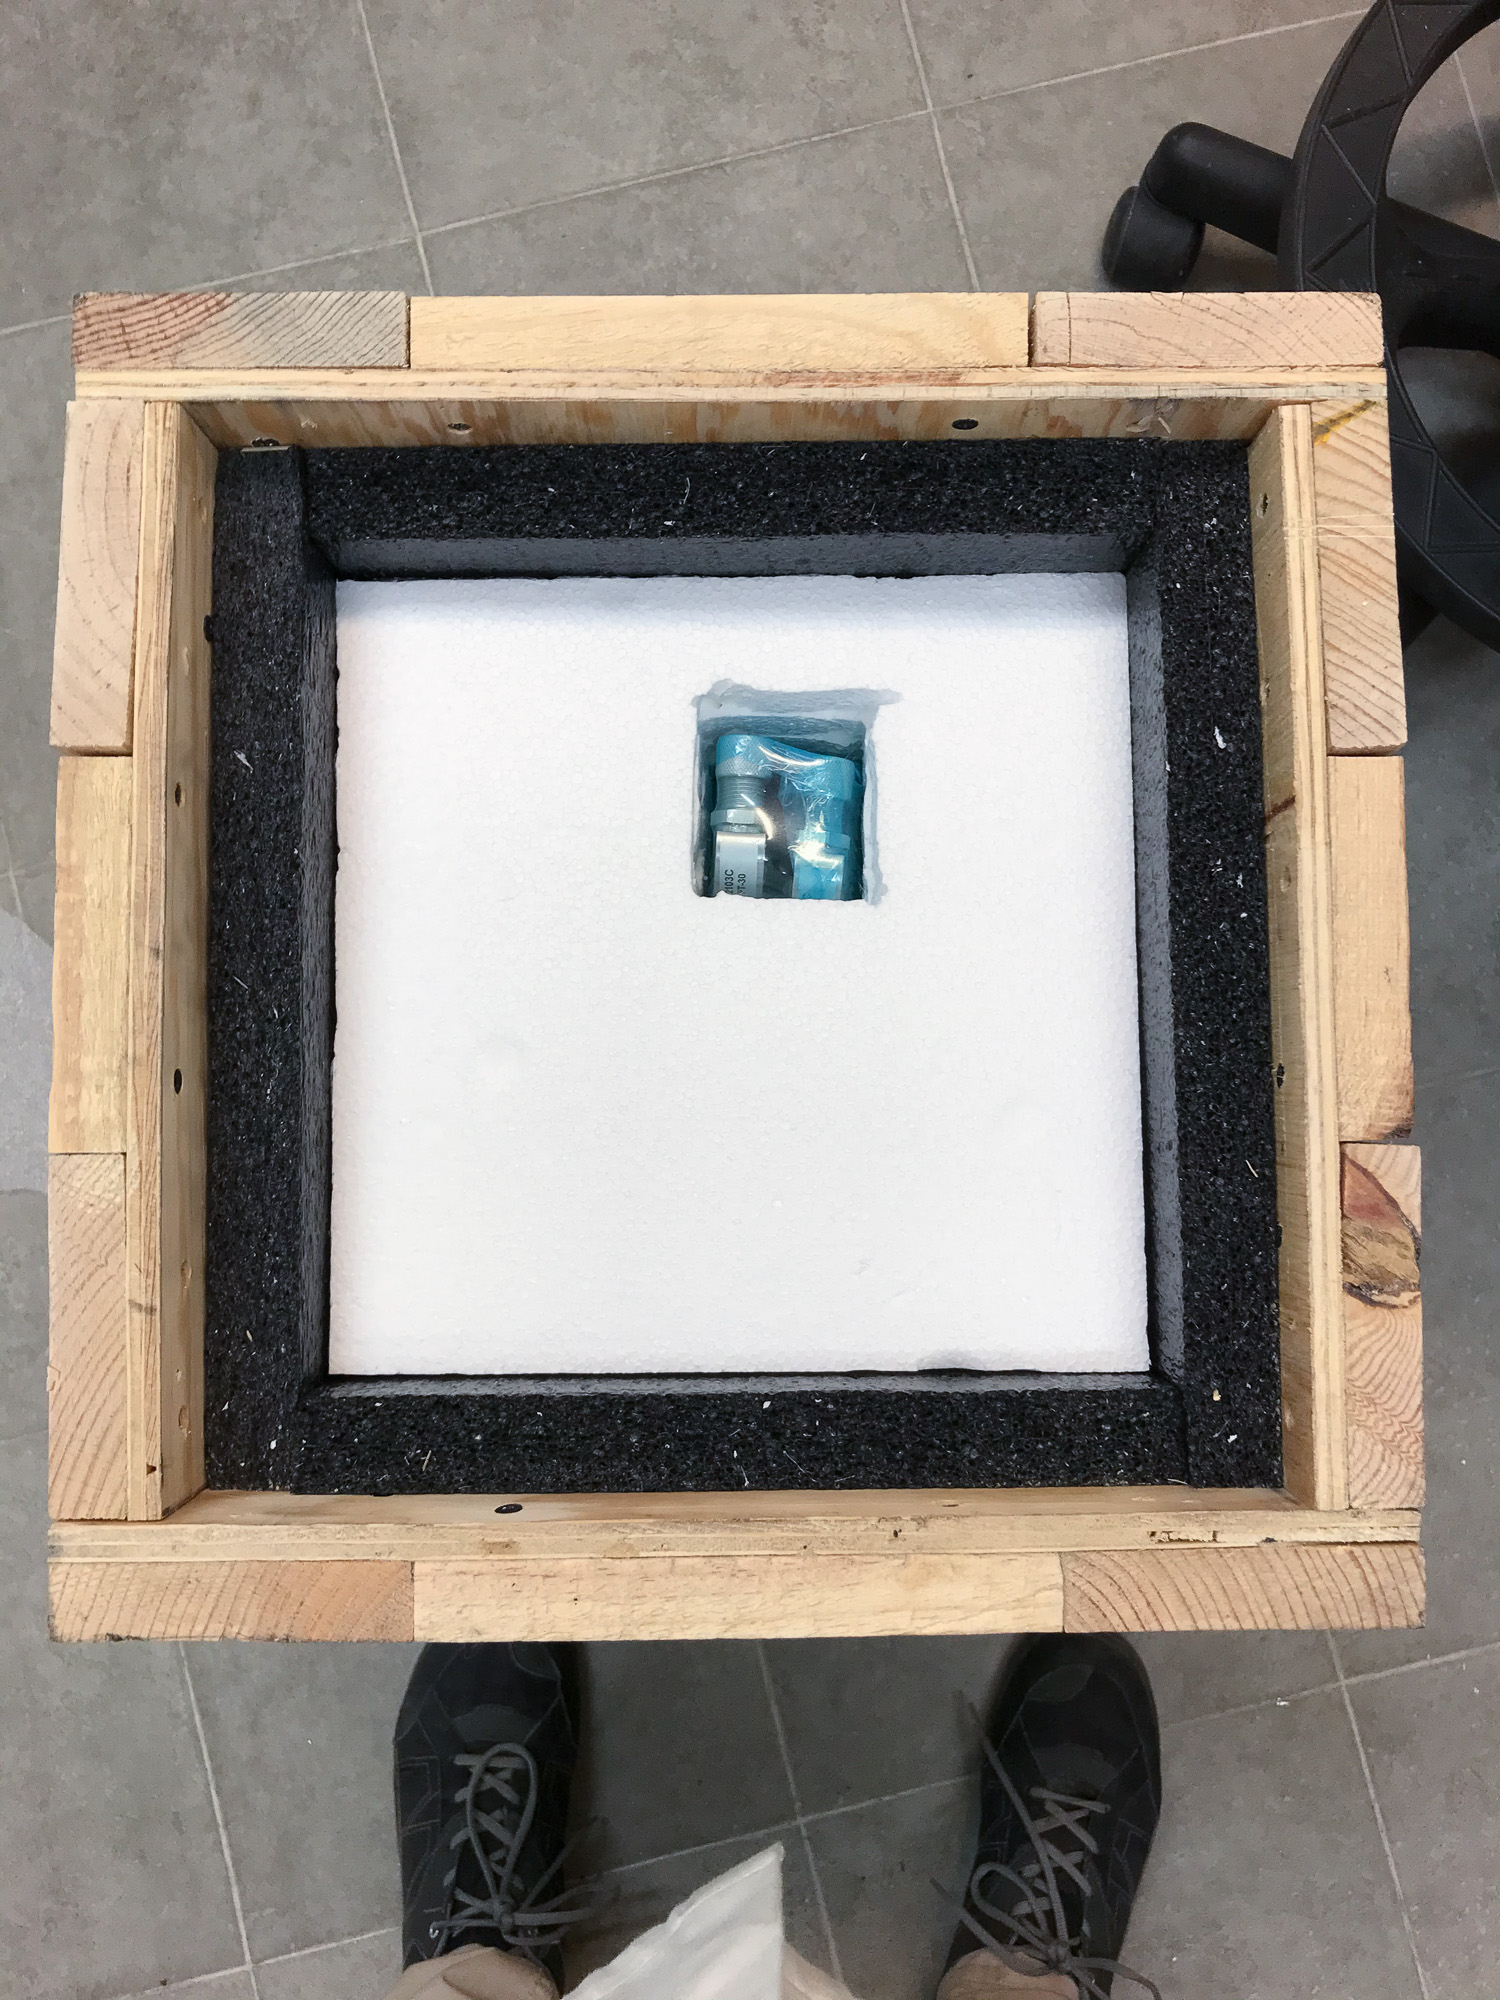
\includegraphics[width=0.30\linewidth]{figures/20201210T120034.jpg}
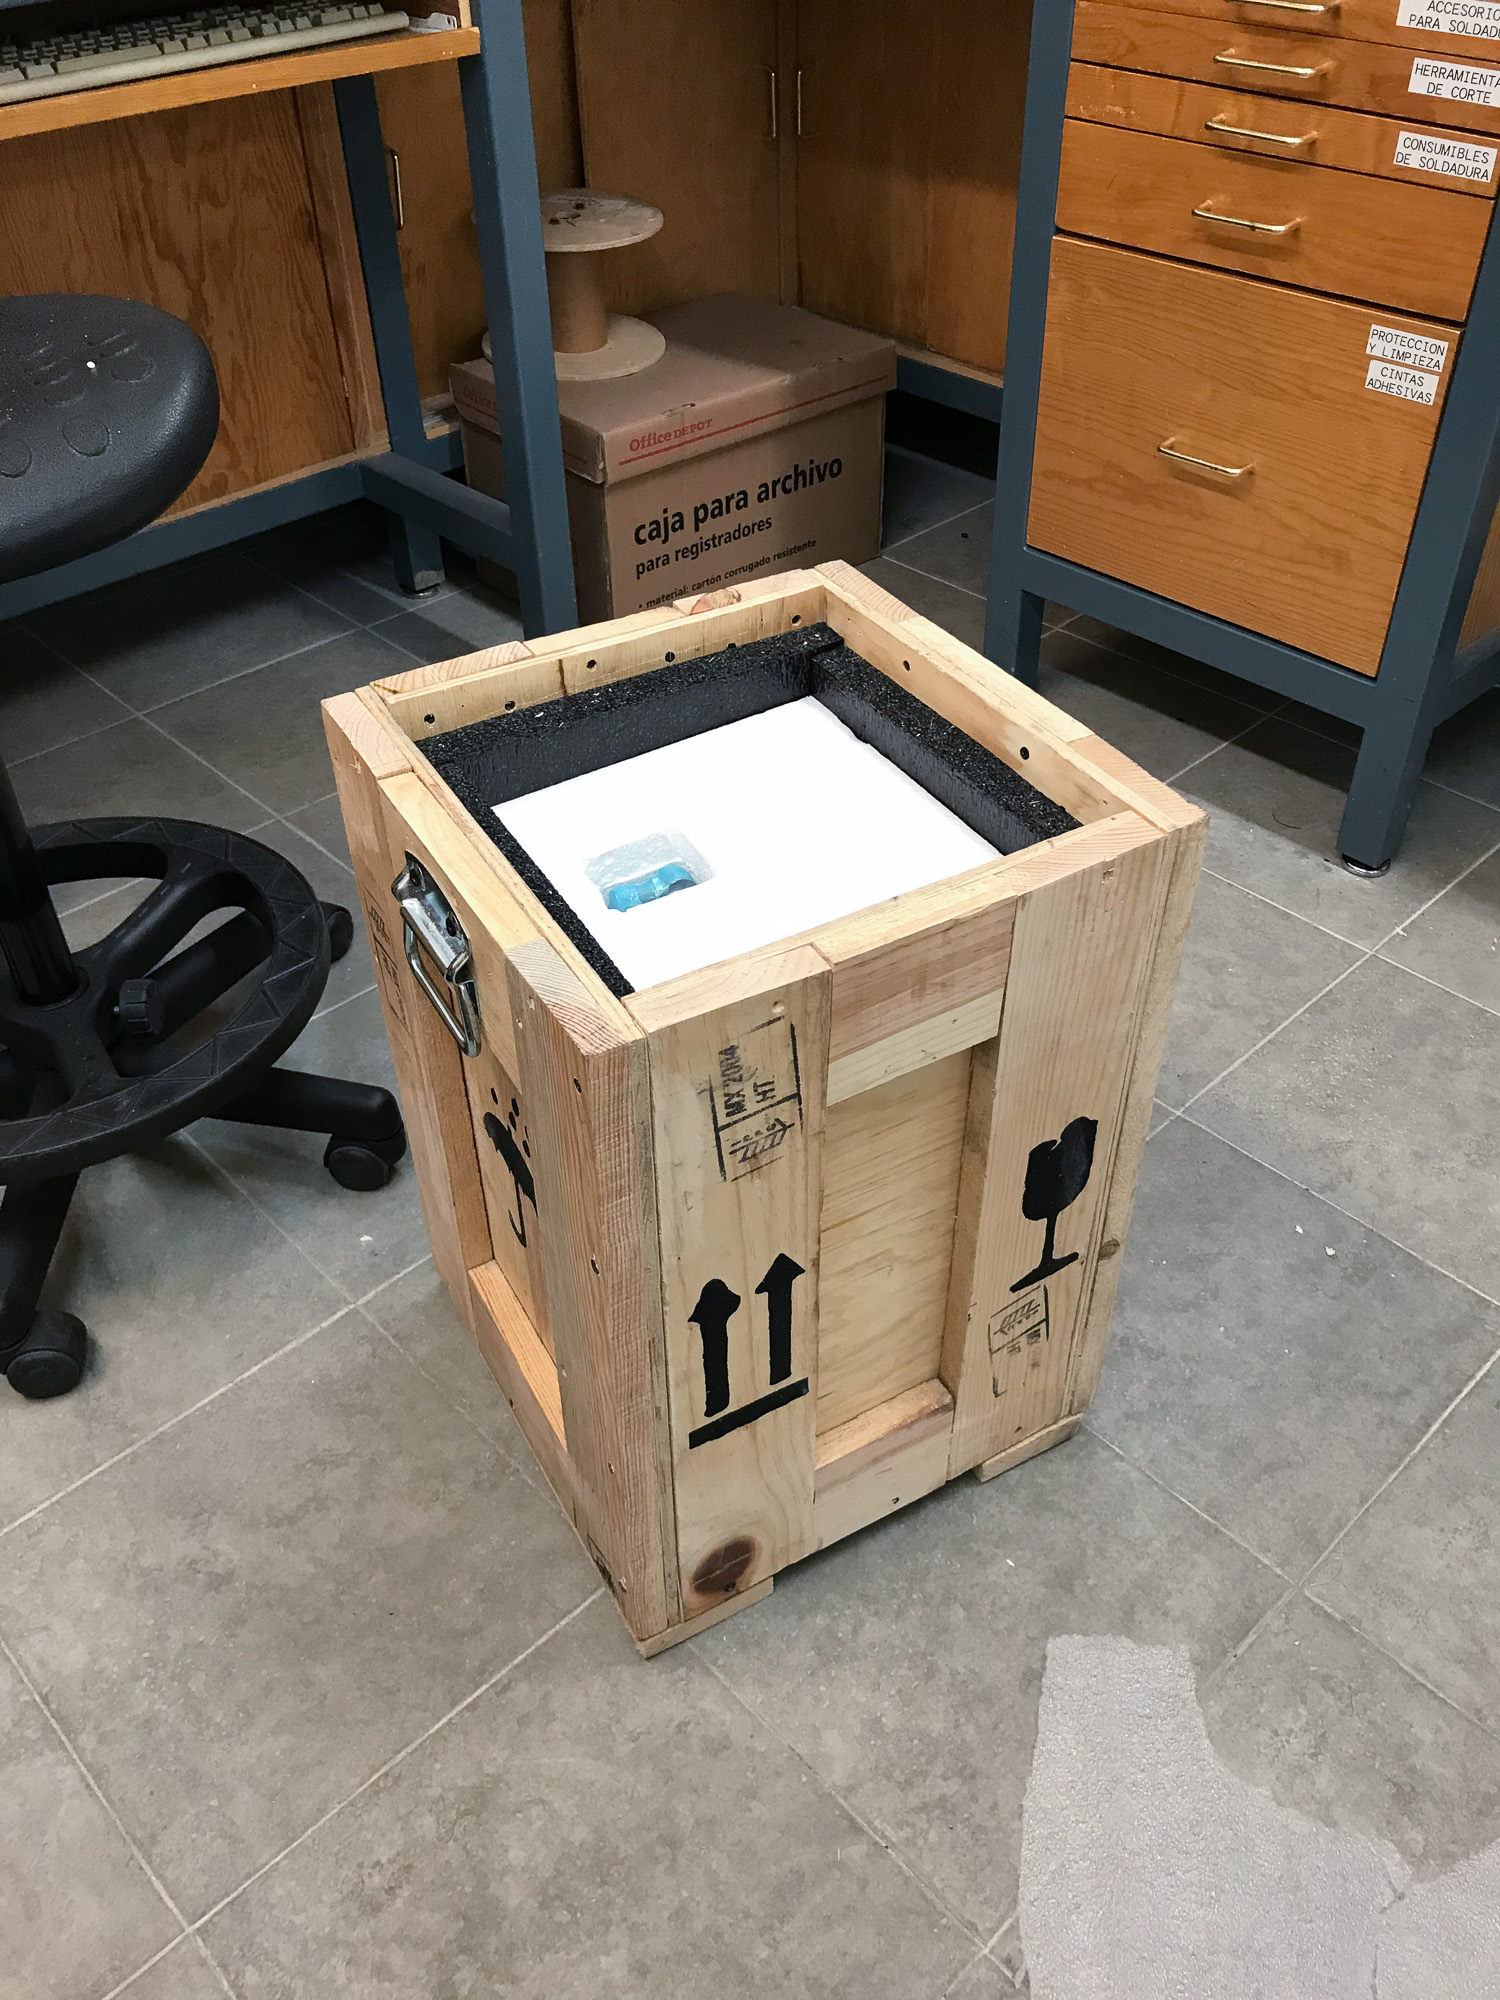
\includegraphics[width=0.30\linewidth]{figures/20201210T120046.jpg}
\end{center}
\caption{Box 2 packing. Left: the CCD is supported from above by foam sheets. The lower one has two holes for the hoses and connectors. Middle. The sheets other than the lower one have only one hole for the hoses. Right: The sheets should reach to the top of the foam.}
\label{figure:box-two-packing}
\end{figure}

\begin{figure}[bp]
\begin{center}
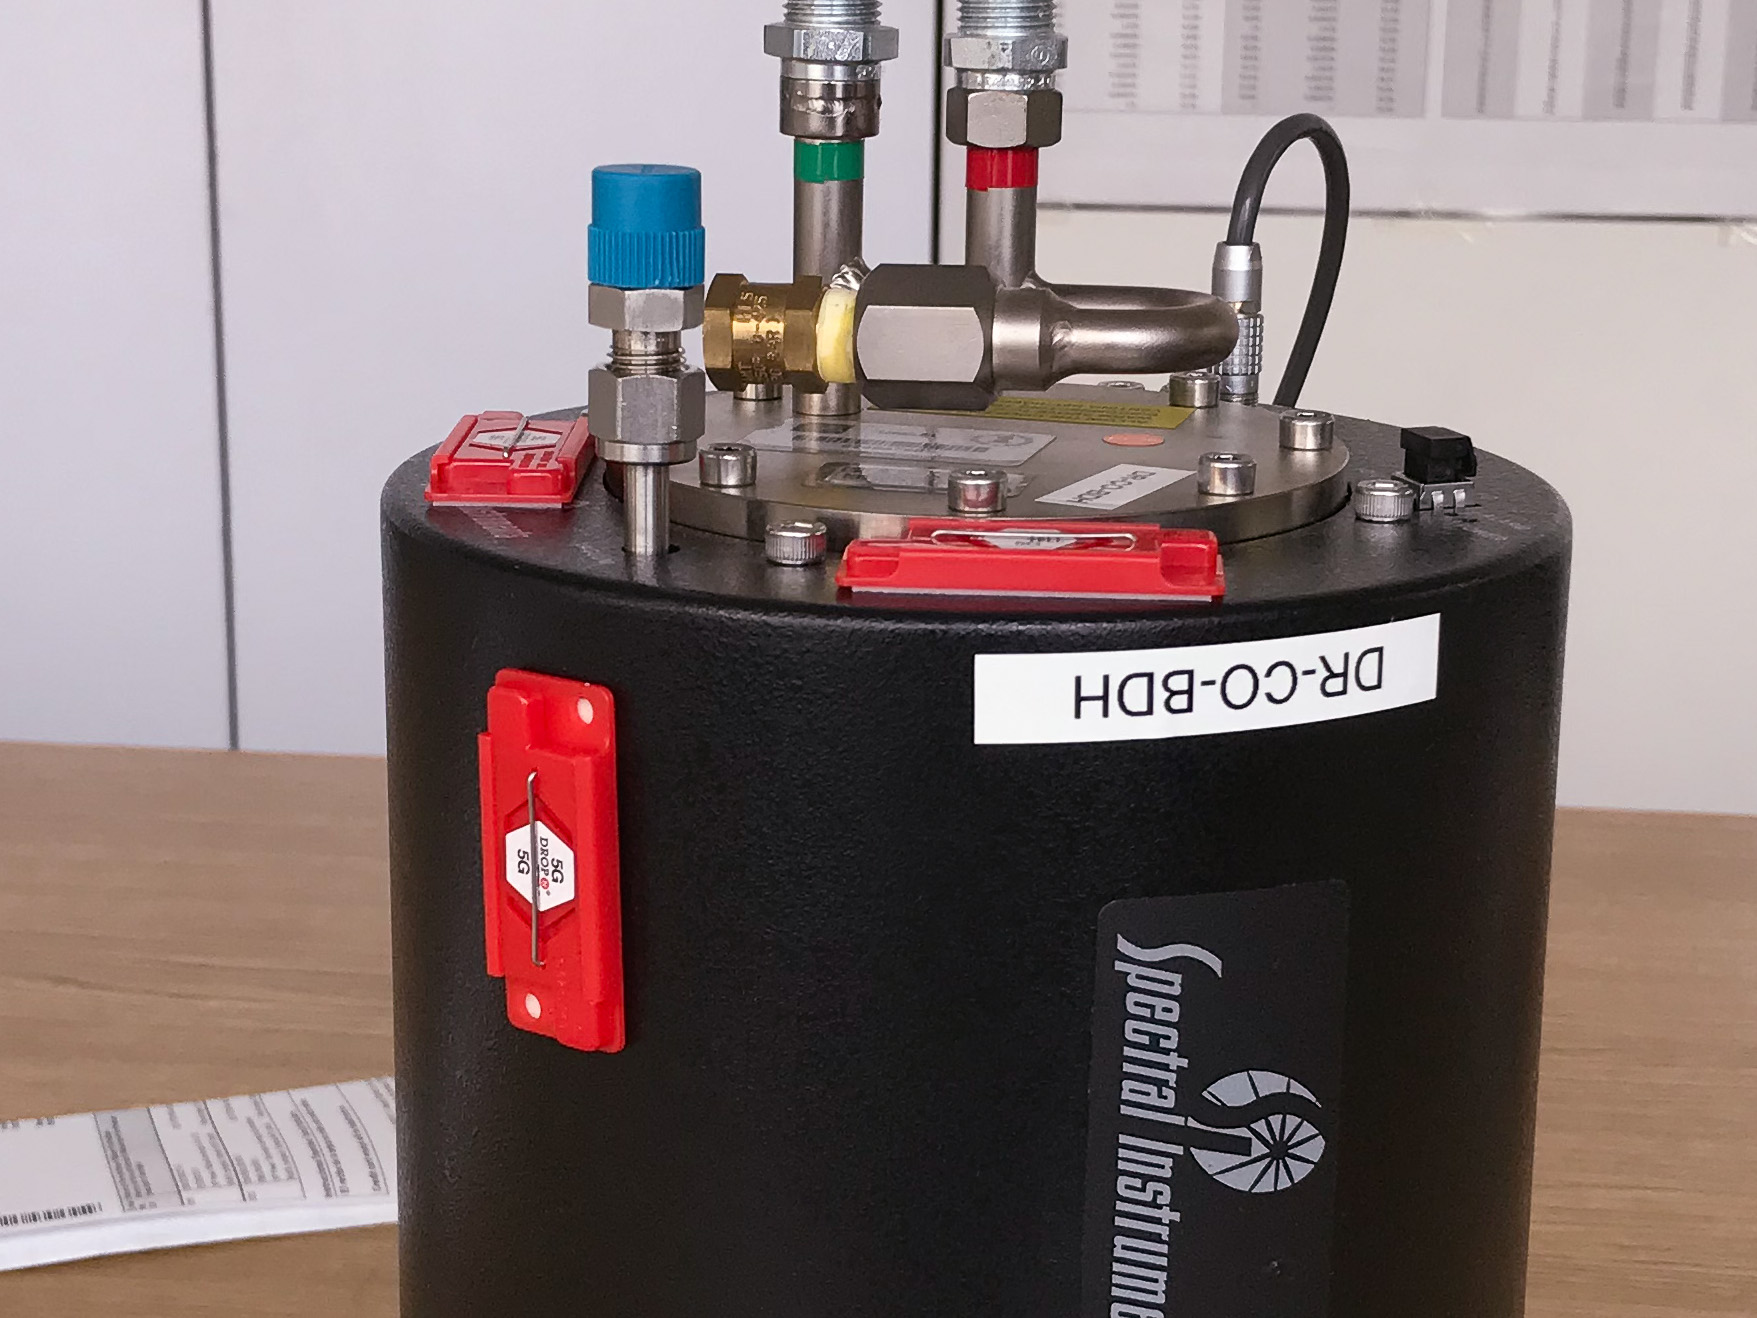
\includegraphics[width=0.3\linewidth]{figures/20201210T100146-2.jpg}
\end{center}
\caption{Box 2 internal 5$g$ sensors.}
\label{figure:box-two-internal-sensors}
\end{figure}


\begin{figure}[bp]
\begin{center}
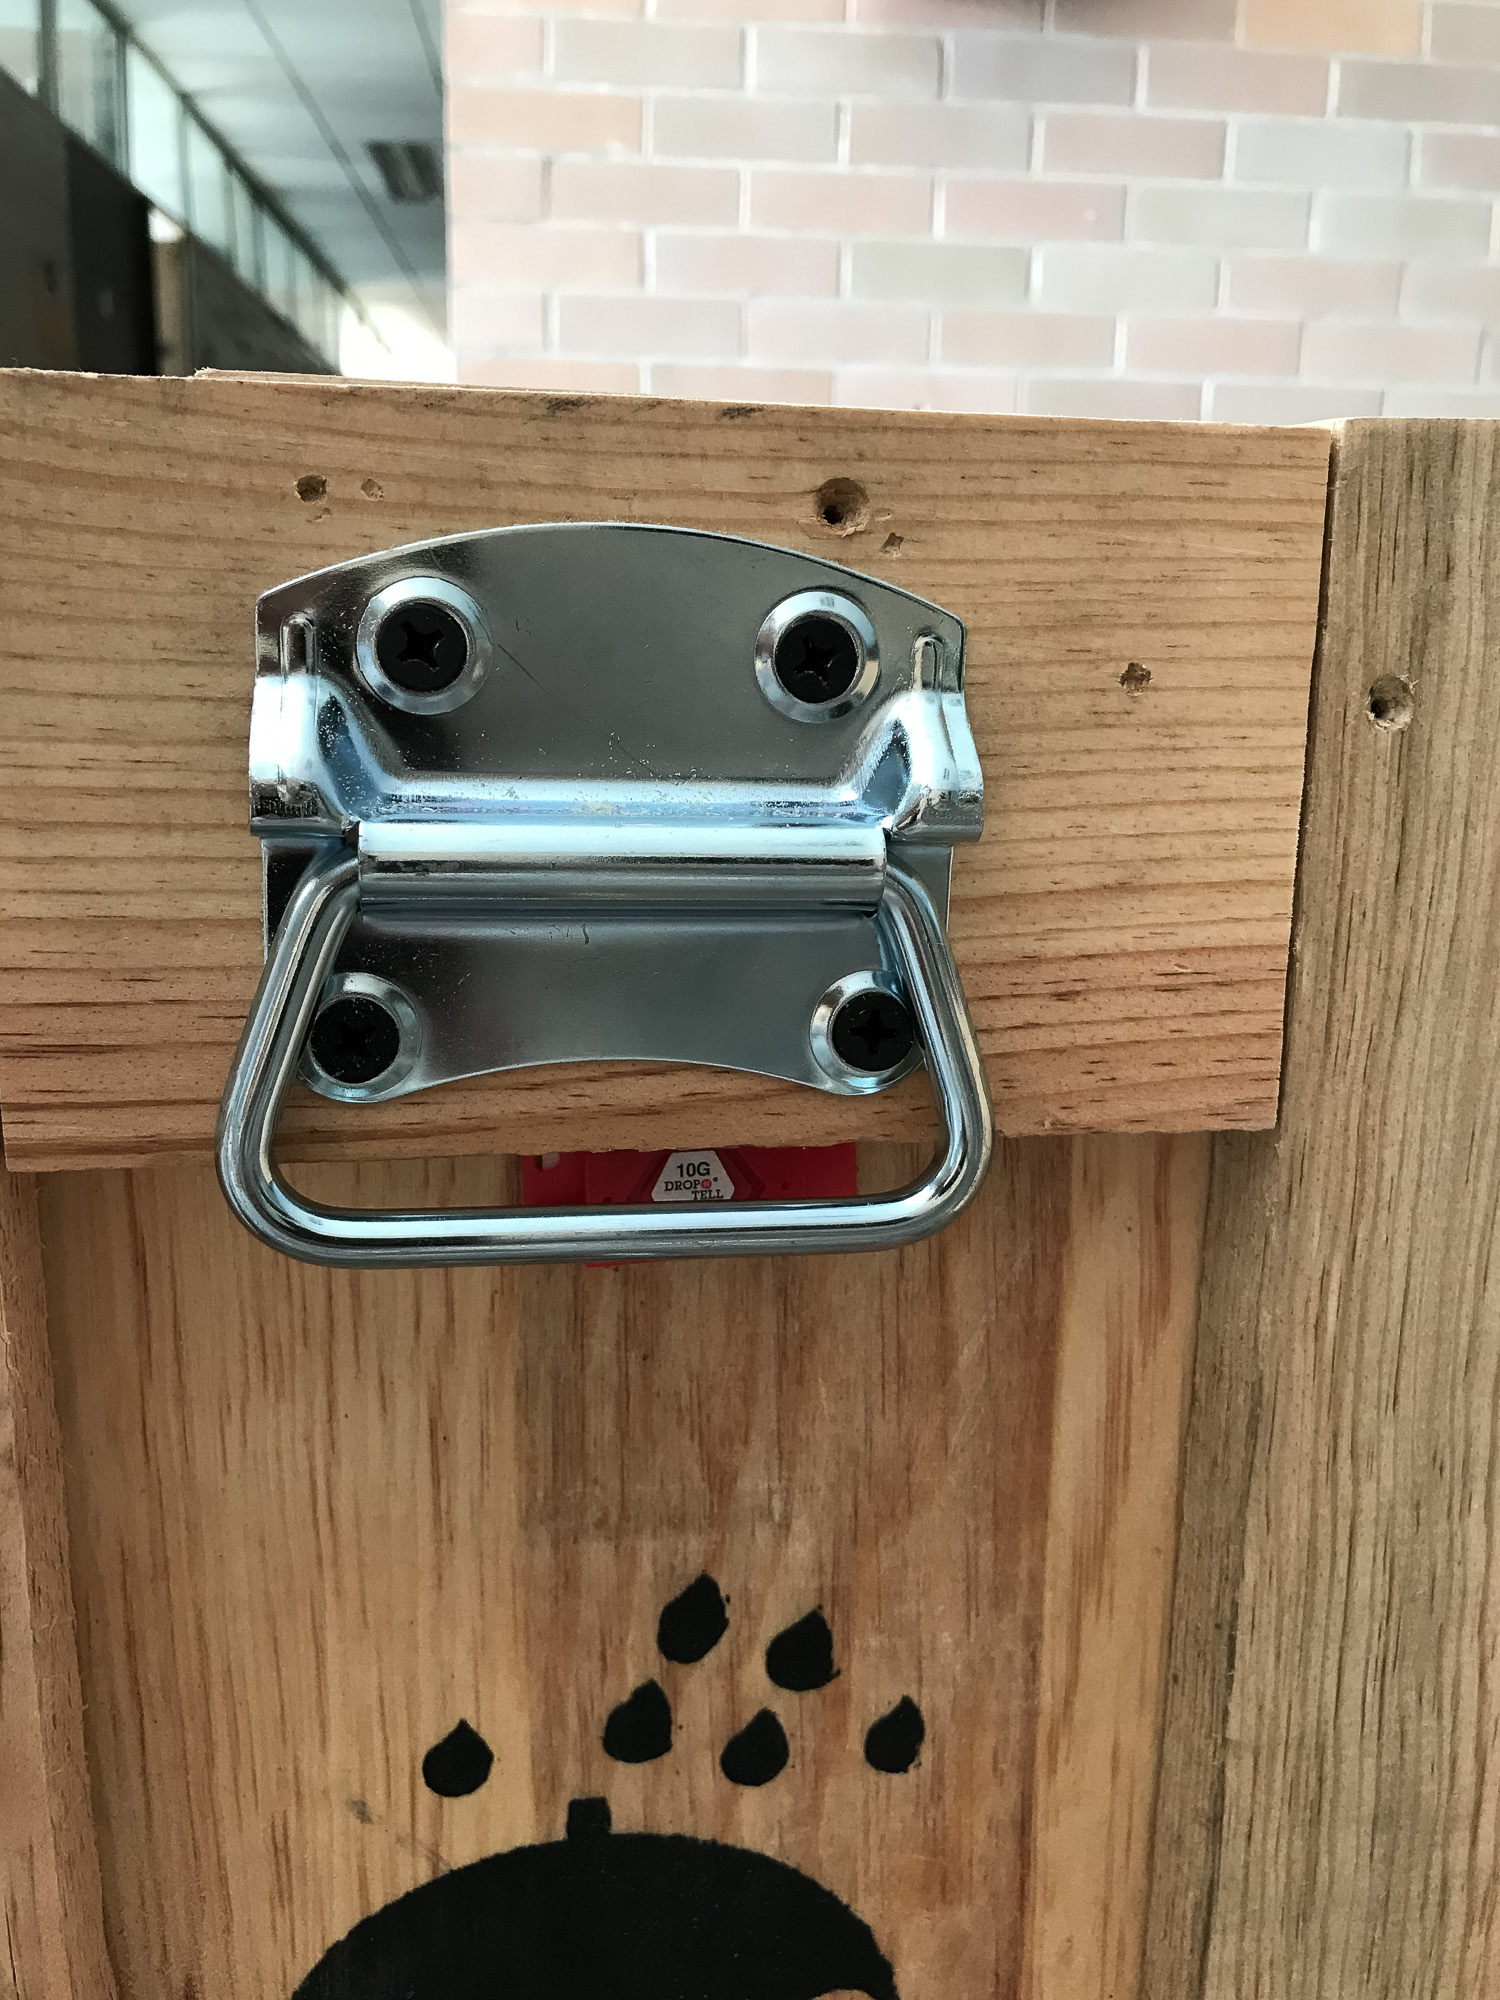
\includegraphics[width=0.3\linewidth]{figures/20210106T113459.jpg}
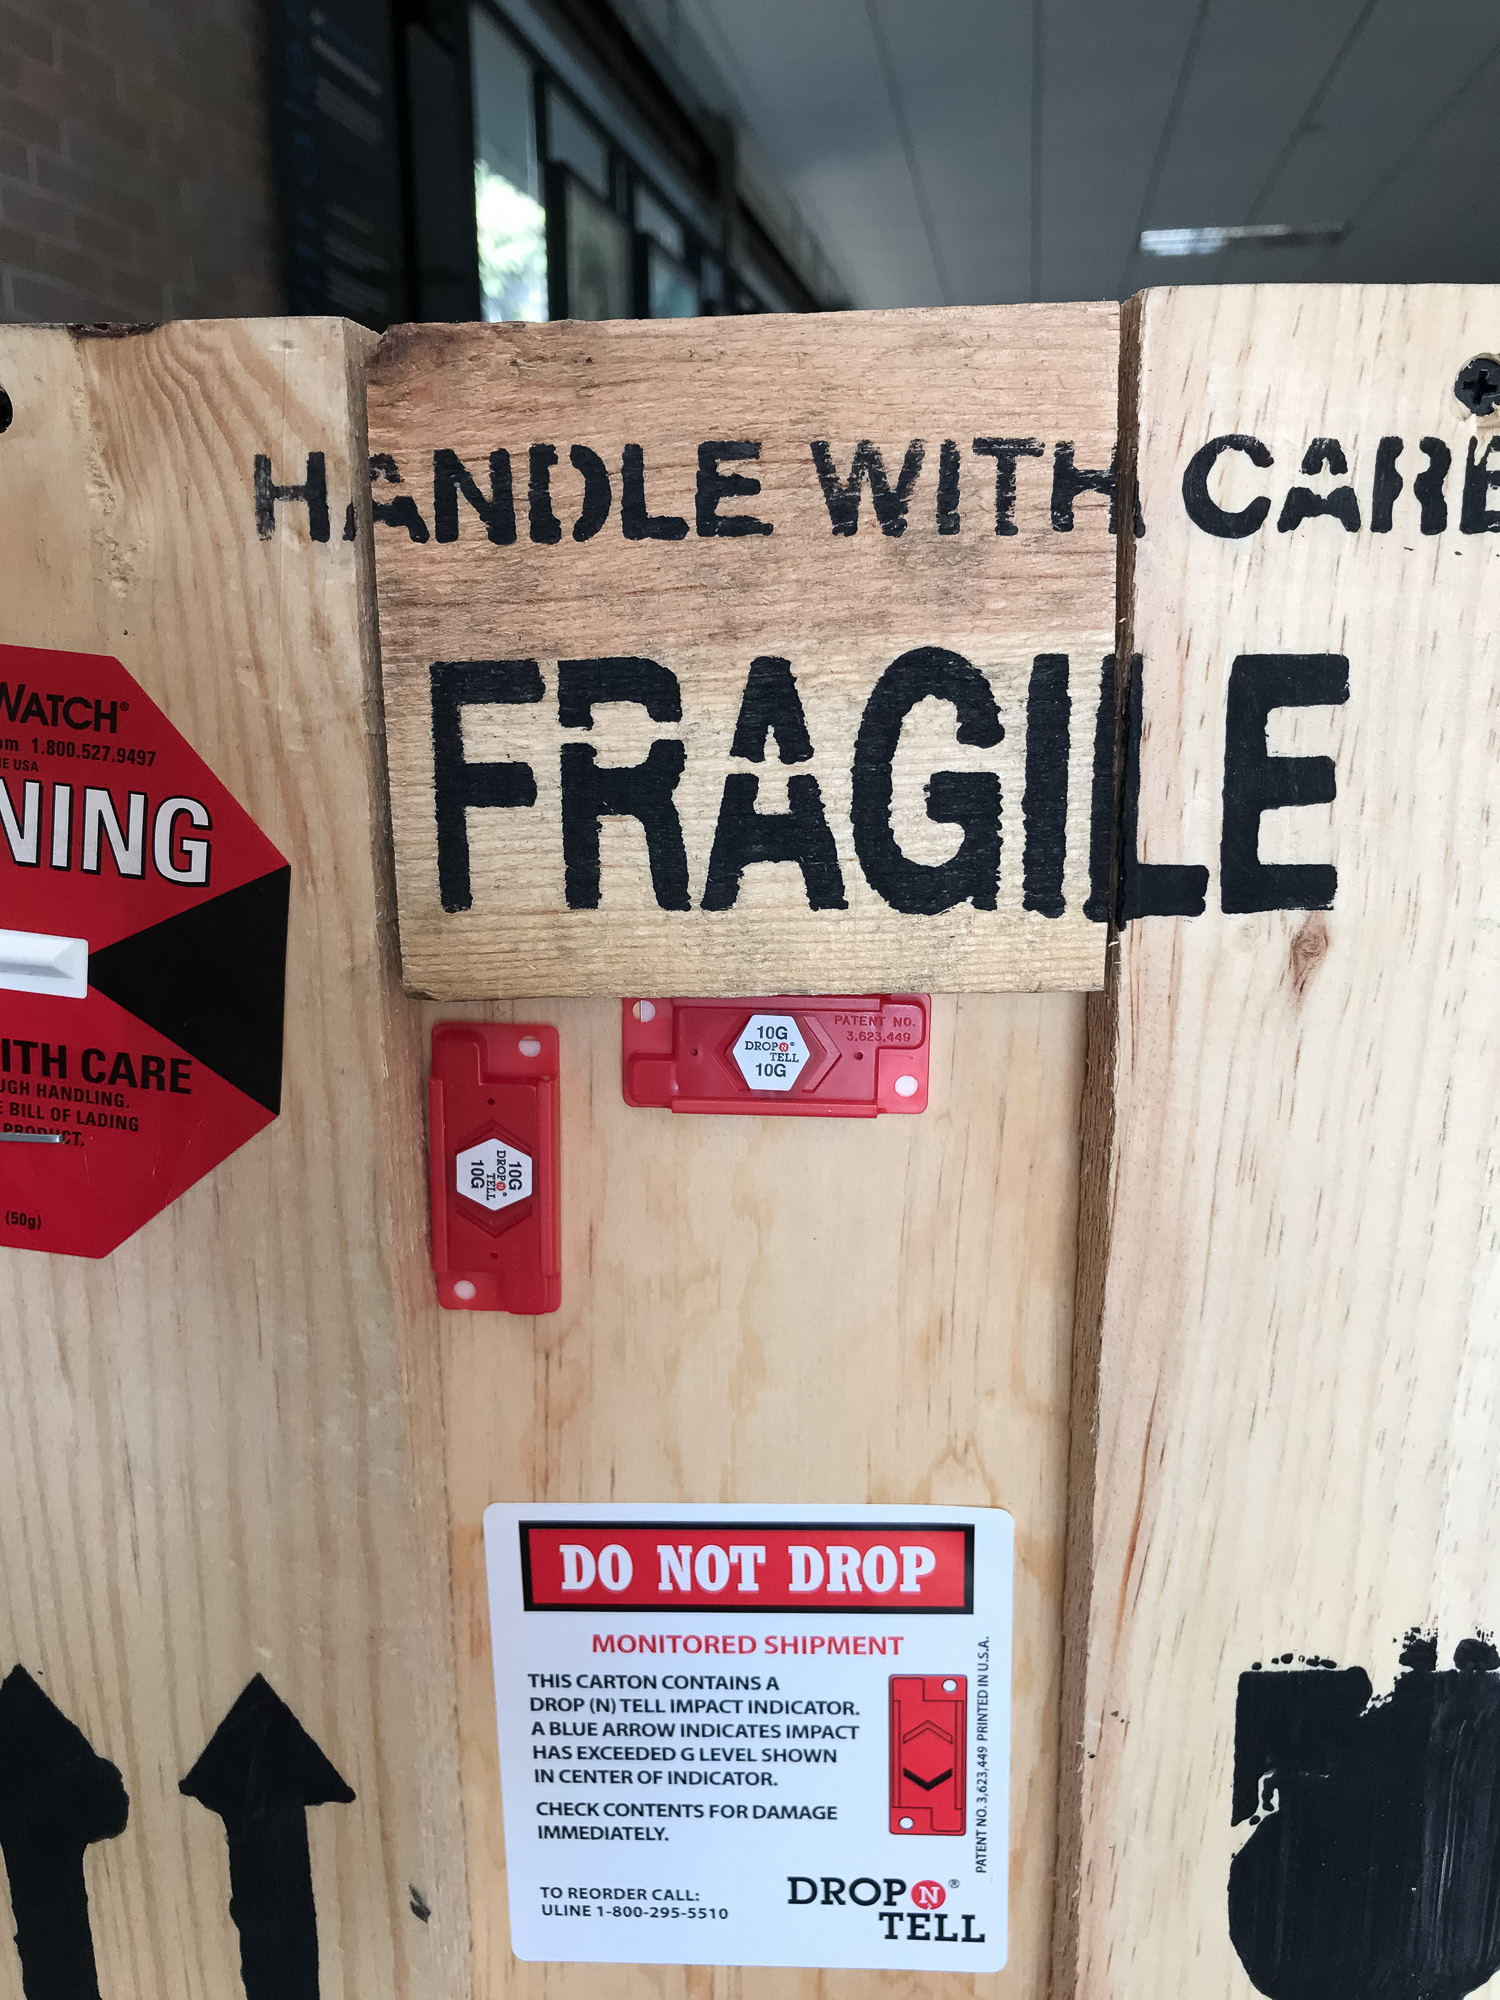
\includegraphics[width=0.3\linewidth]{figures/20210106T113452.jpg}
\end{center}
\caption{Box 2 external sensors. Left: one of the three 10$g$ sensors and the temperature sensors. Right: the other two 10$g$ sensors.}
\label{figure:box-two-external-sensors}
\end{figure}


\subsection{Description}

Box 2 contains:

\begin{itemize}
    \item The blue detector head DR-CO-BDH (with the detector DR-CO-BDT and window DR-CO-BDW).
    \item The blue detector head front cover DR-CO-BDH-FC.
\end{itemize}

The box is a custom-made wooden crate and is lined with foam.  See Figure~\ref{figure:box-two}.

The box has three 10-g impact indicators on the outside (see Figure~\ref{figure:box-two-external-sensors}) and the detector head has three 5-g indicators (see Figure~\ref{figure:box-two-internal-sensors}).

Box 2 is $38 \times 38 \times 55$ cm ($L \times W \times H$) and has a weight of 24 kg.

\subsection{Unpacking Instructions}

\begin{enumerate}
\item Verify that the external 10-g impact indicators are not activated. If they are, consult with the UNAM team before proceeding further.
\item Remove the 8 screws that fasten the lid of the box. Remove the lid.
\item Remove the foam sheets between the top of the detector head and the box. See Figure~\ref{figure:box-two-packing}.
\item Lift the detector head from the box.
\item Verify that the internal 5-g impact indicators are not activated. If they are, consult with the UNAM team before proceeding further.
\item Fasten the lid in place with the 8 screws.
\end{enumerate}

\subsection{Repacking Instructions}

\begin{enumerate}
\item Verify that the external 10-g and internal 5-g impact indicators are not activated. If they are, replace them with spares from Box 28.
\item Make sure the front cover is installed.
\item Wrap the detector head in plastic.
\item Place the detector head in the box with the cover on the bottom. Surround it with foam. Add dessicant.
\item Place the specially-cut foam sheets above the detector head, with the holes lined up with the hoses and connectors. Note that the lower one has two holes and the rest have only one hole.
\item Fasten the lid in place with the 8 screws.
\end{enumerate}

%%%%%%%%%%%%%%%%%%%%%%%%%%%%%%%%%%%%%%%%%

\clearpage
\section{Box 3}

\begin{figure}[bp]
\begin{center}
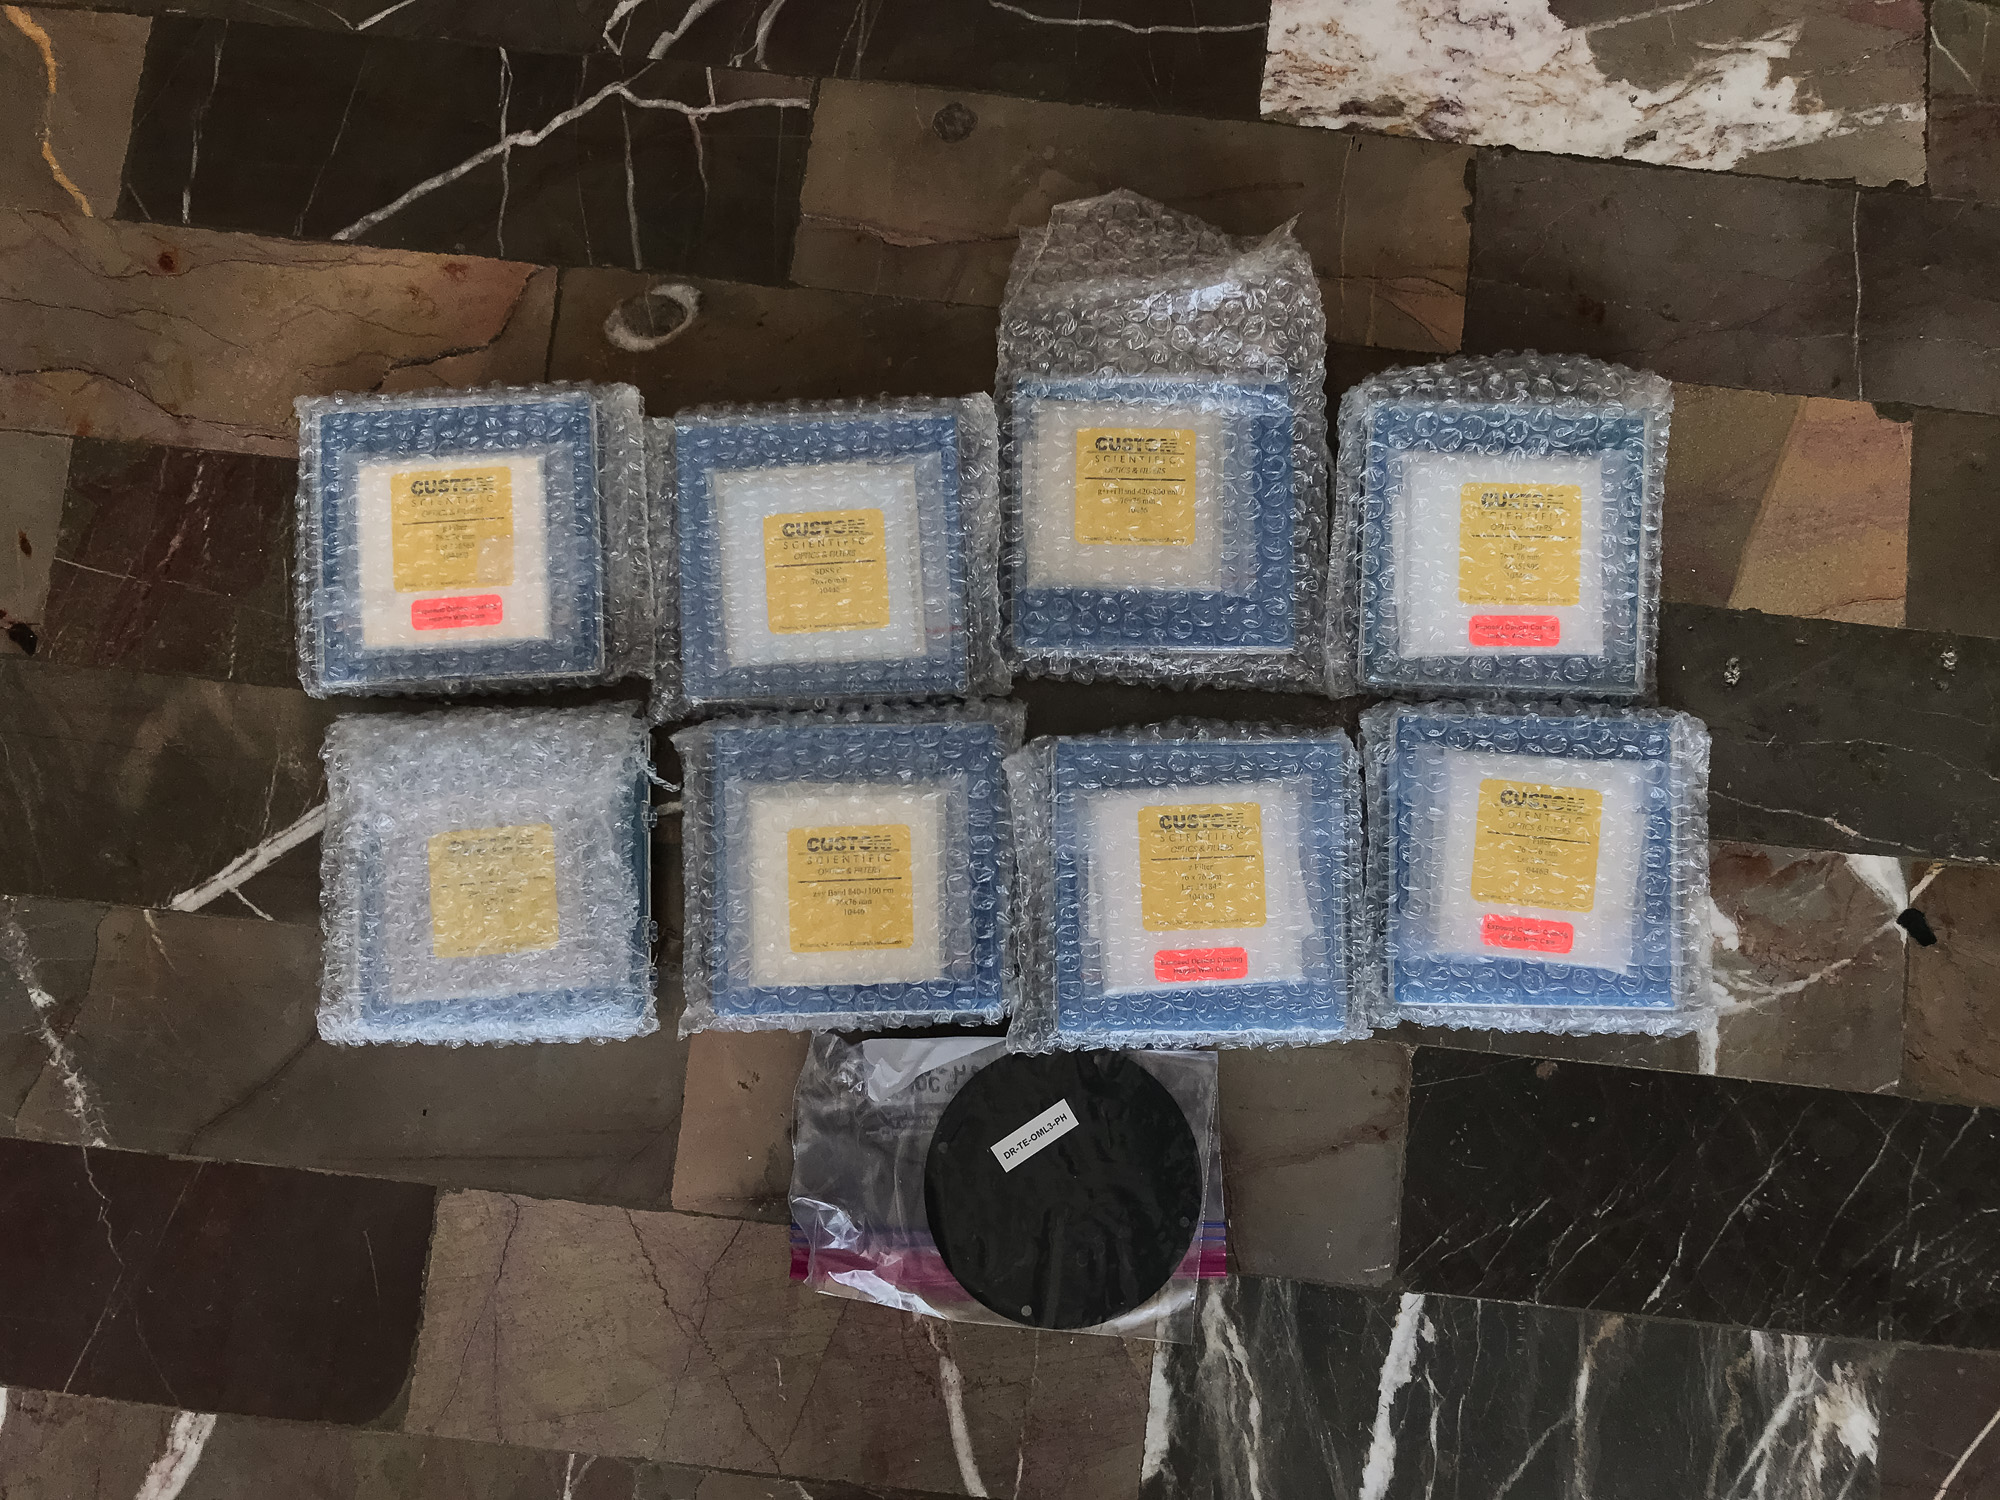
\includegraphics[width=0.60\linewidth]{figures/20210106T114617.jpg}
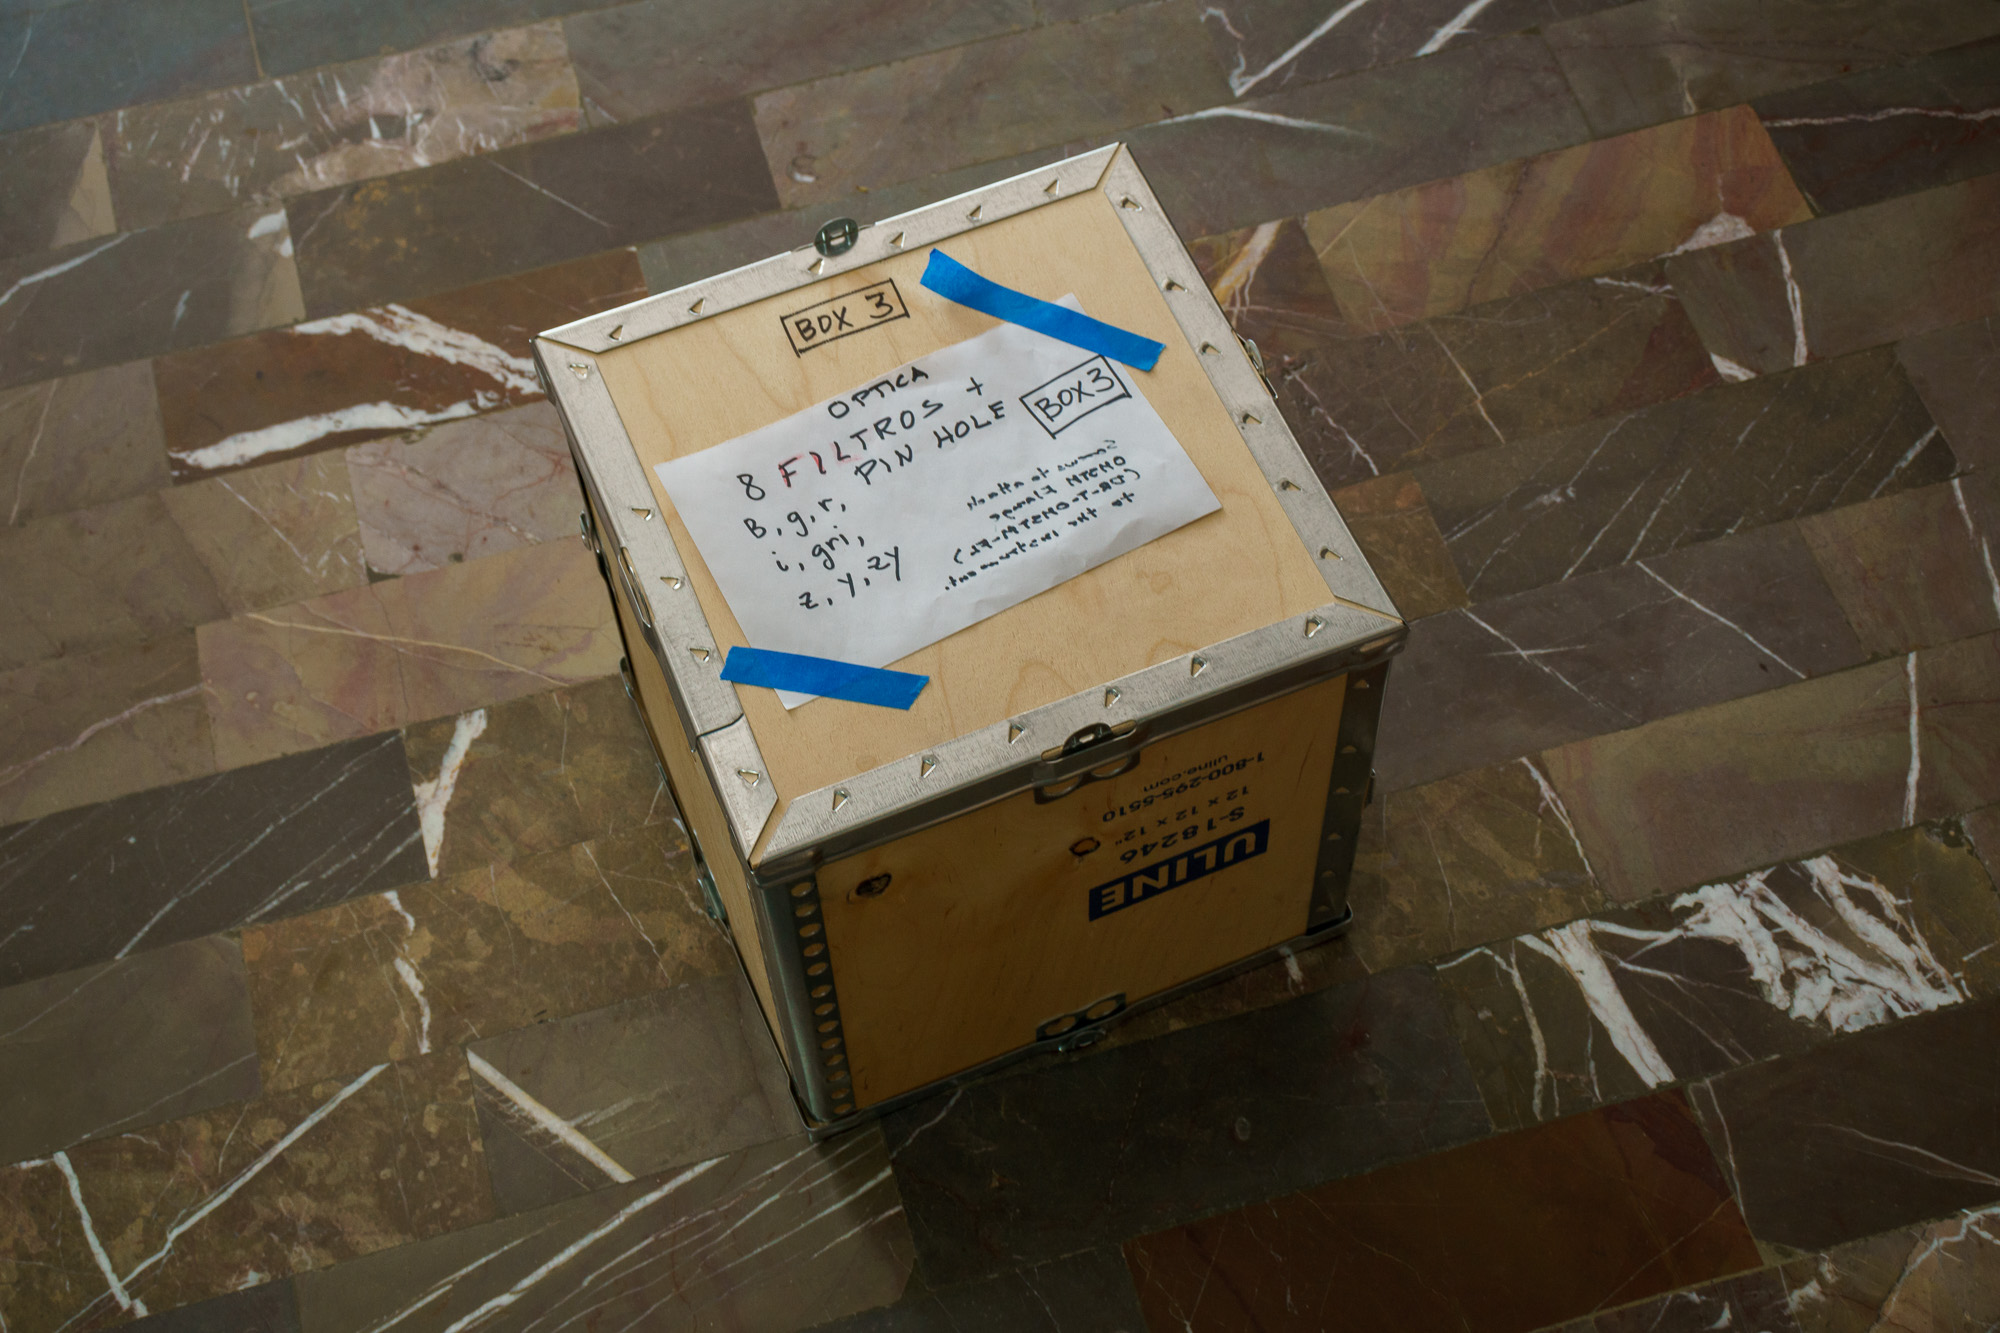
\includegraphics[width=0.60\linewidth]{figures/20201209T114446.jpg}
\end{center}
\caption{Box 3 and its contents.}
\label{figure:box-three}
\end{figure}

\begin{figure}[bp]
\begin{center}
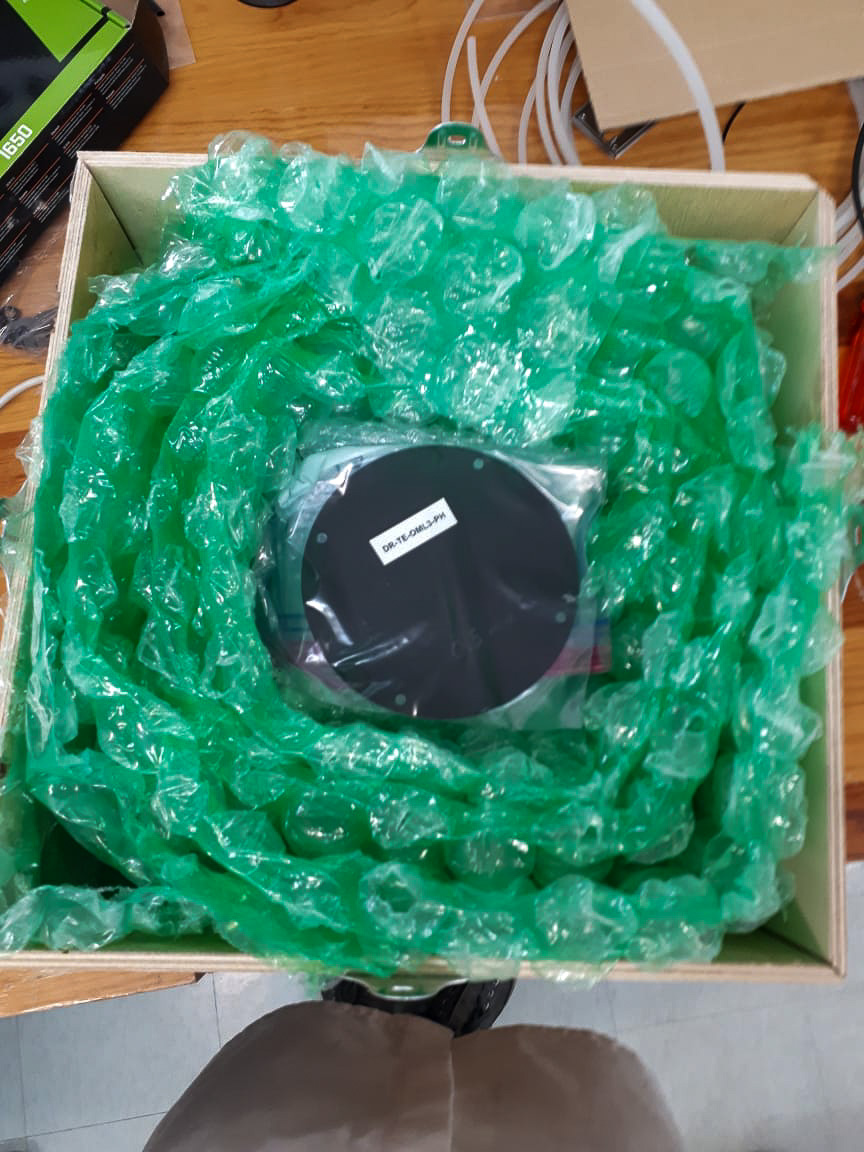
\includegraphics[width=0.40\linewidth]{figures/20201209T080439.jpg}
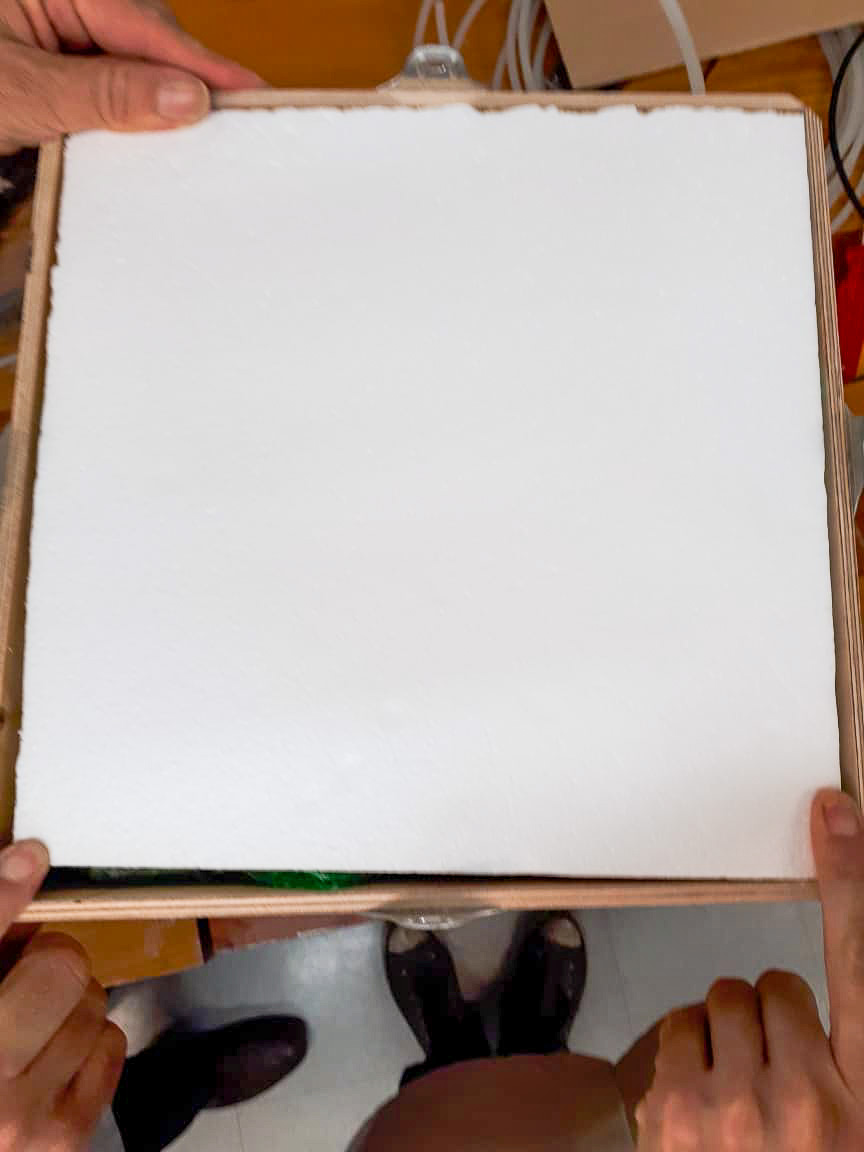
\includegraphics[width=0.40\linewidth]{figures/20201209T080445.jpg}
\end{center}
\caption{Box 3 packing. Left. The contents are wrapped in bubble wrap. Right. There are foam sheets above and below the contents.}
\label{figure:box-three-packing}
\end{figure}

\subsection{Description}

Box 3 contains:

\begin{itemize}
\item The eight filters DR-OP-FL-B, DR-OP-FL-G, DR-OP-FL-R, DR-OP-FL-I, DR-OP-FL-GRI, DR-OP-FL-Z, DR-OP-FL-Y, and DR-OP-FL-ZY.
\item The pinhole DR-TE-OML3-PH.
\end{itemize}

The box is a commercial plywood box with external steel reinforcement. The filters are housed in protected by individual plastic boxes. The contents as a whole are protected by bubble-wrap and foam sheets. See Figure~\ref{figure:box-three}.

Box 3 is $30 \times 30 \times 30$ cm ($L \times W \times H$) and has a weight of 4 kg.

\subsection{Unpacking Instructions}

\begin{enumerate}
\item Bend the tabs and remove the lid.
\item Unpack the contents.
\item Replace the lid.
\end{enumerate}

\subsection{Repacking Instructions}

\begin{enumerate}
\item Place a foam sheet at the bottom of the box. See Figure~\ref{figure:box-three-packing}.
\item Wrap the filters and pinhole in bubble wrap and place them in the box.  See Figure~\ref{figure:box-three-packing}.
\item Place a foam sheet over the contents.  See Figure~\ref{figure:box-three-packing}.
\item Install the lid and bend the tabs to fasten it in place.
\end{enumerate}

%%%%%%%%%%%%%%%%%%%%%%%%%%%%%%%%%%%%%%%%%

\clearpage
\section{Box 4}

\begin{figure}[bp]
\begin{center}
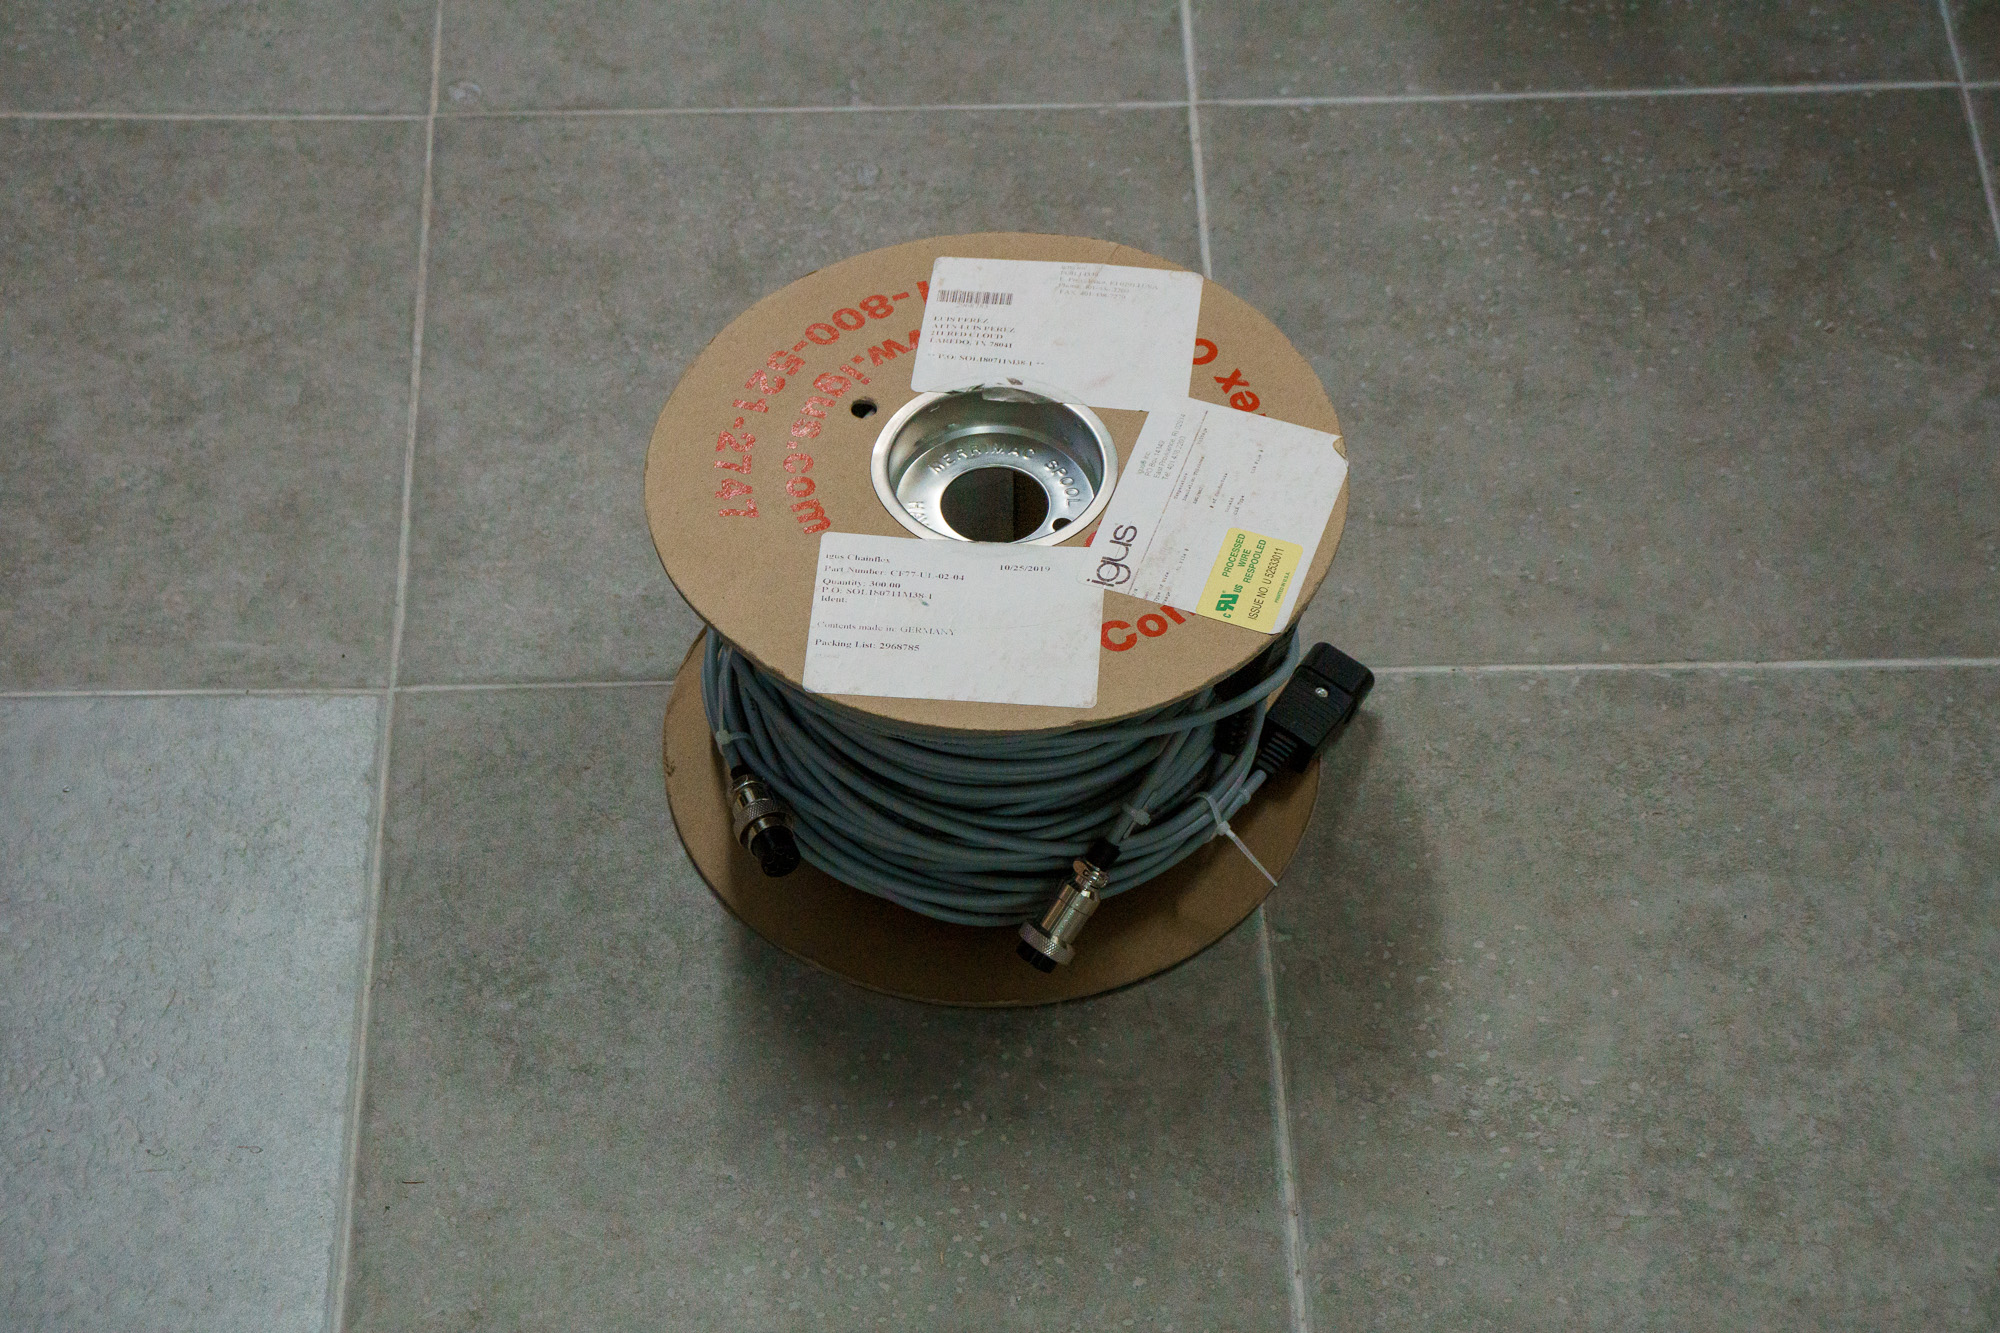
\includegraphics[width=0.60\linewidth]{figures/20201207T185429.jpg}\\[\smallskipamount]
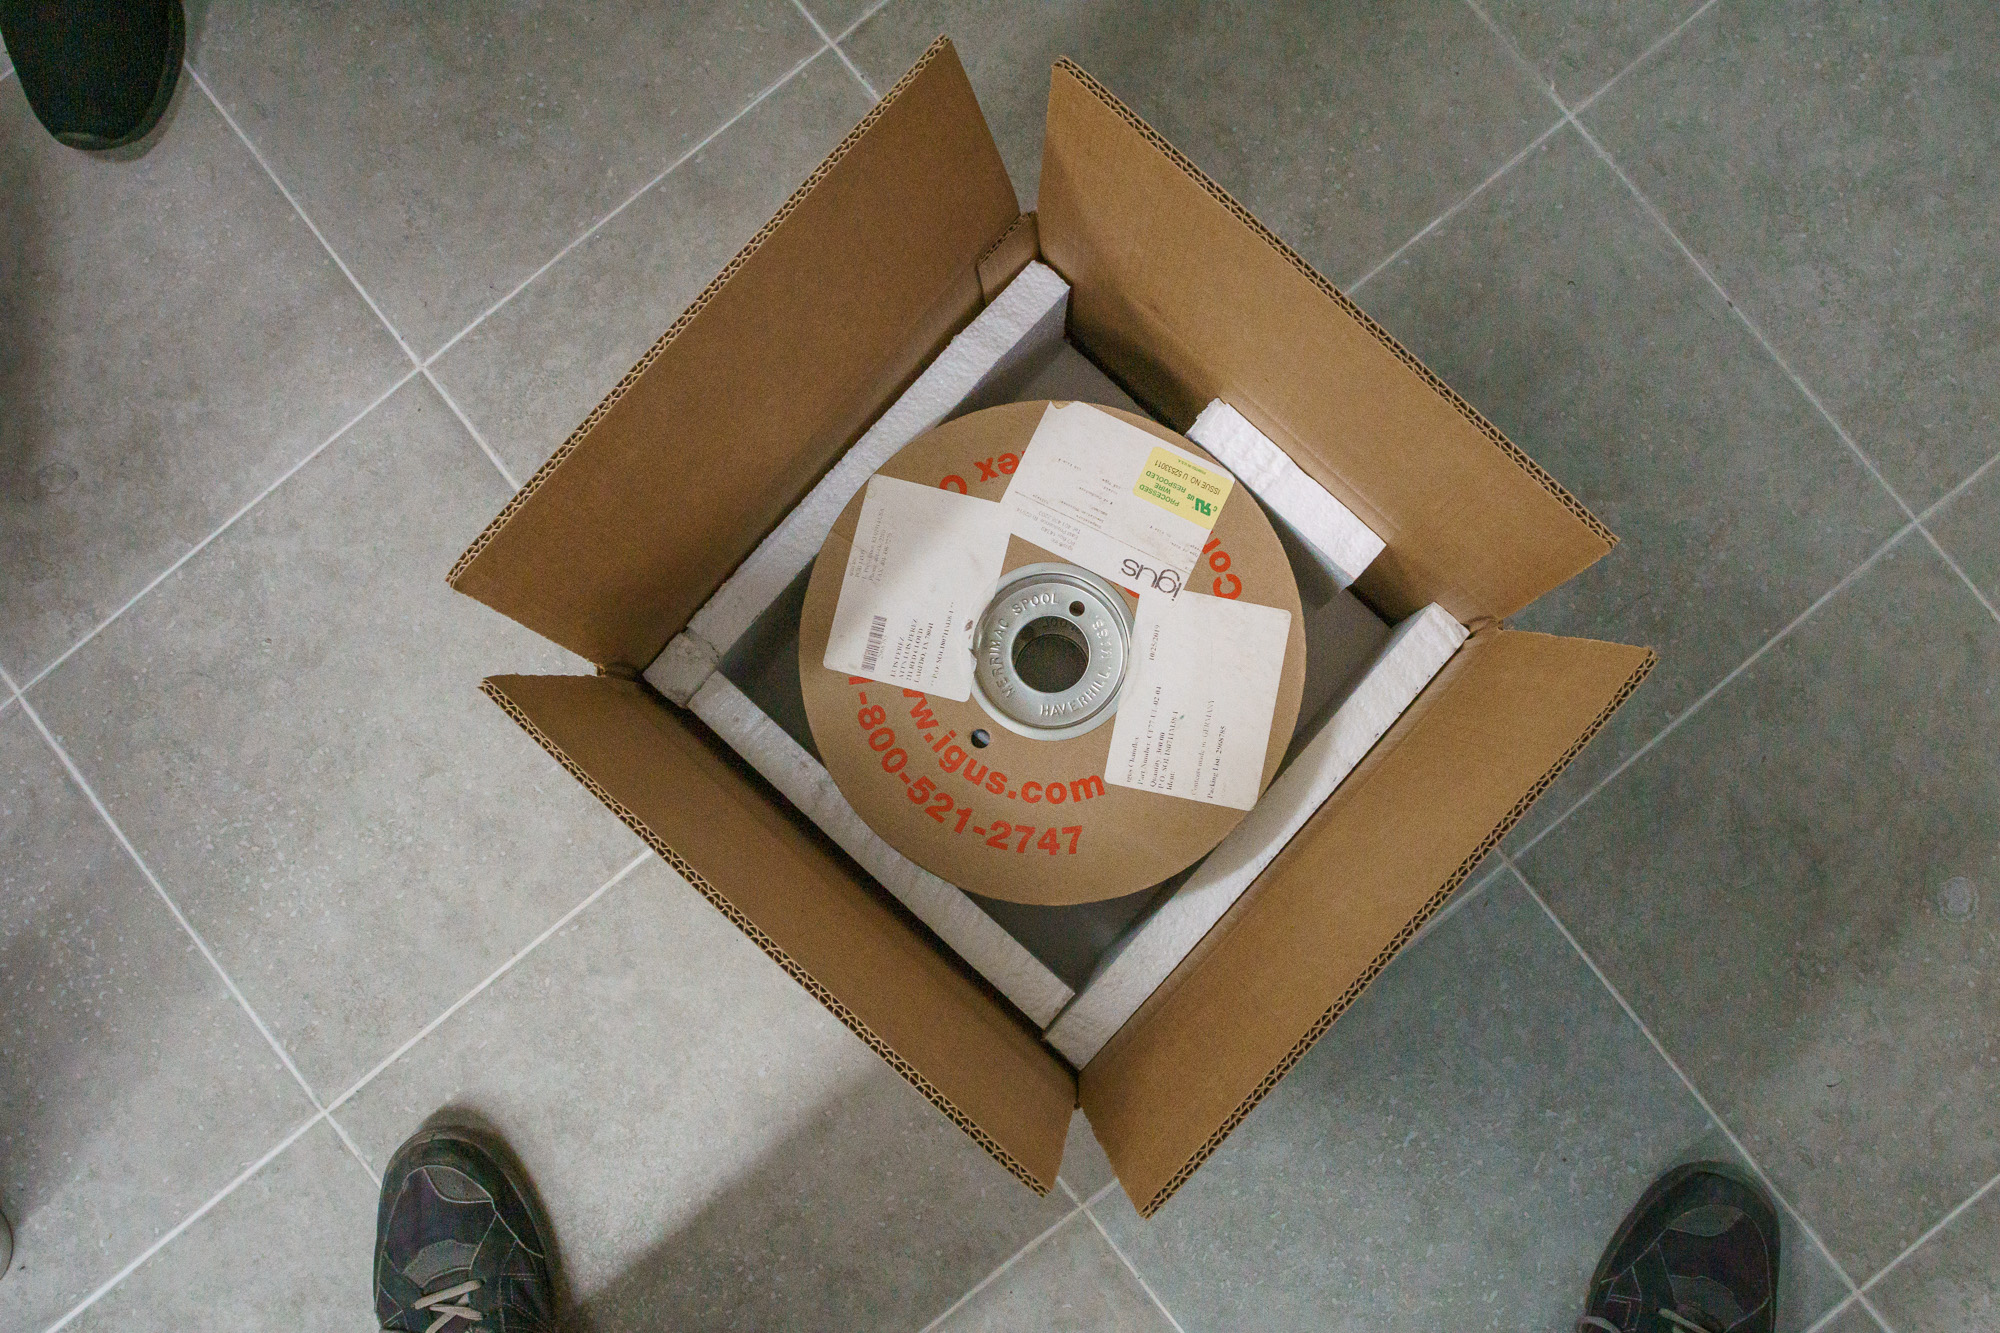
\includegraphics[width=0.60\linewidth]{figures/20201207T185824.jpg}\\[\smallskipamount]
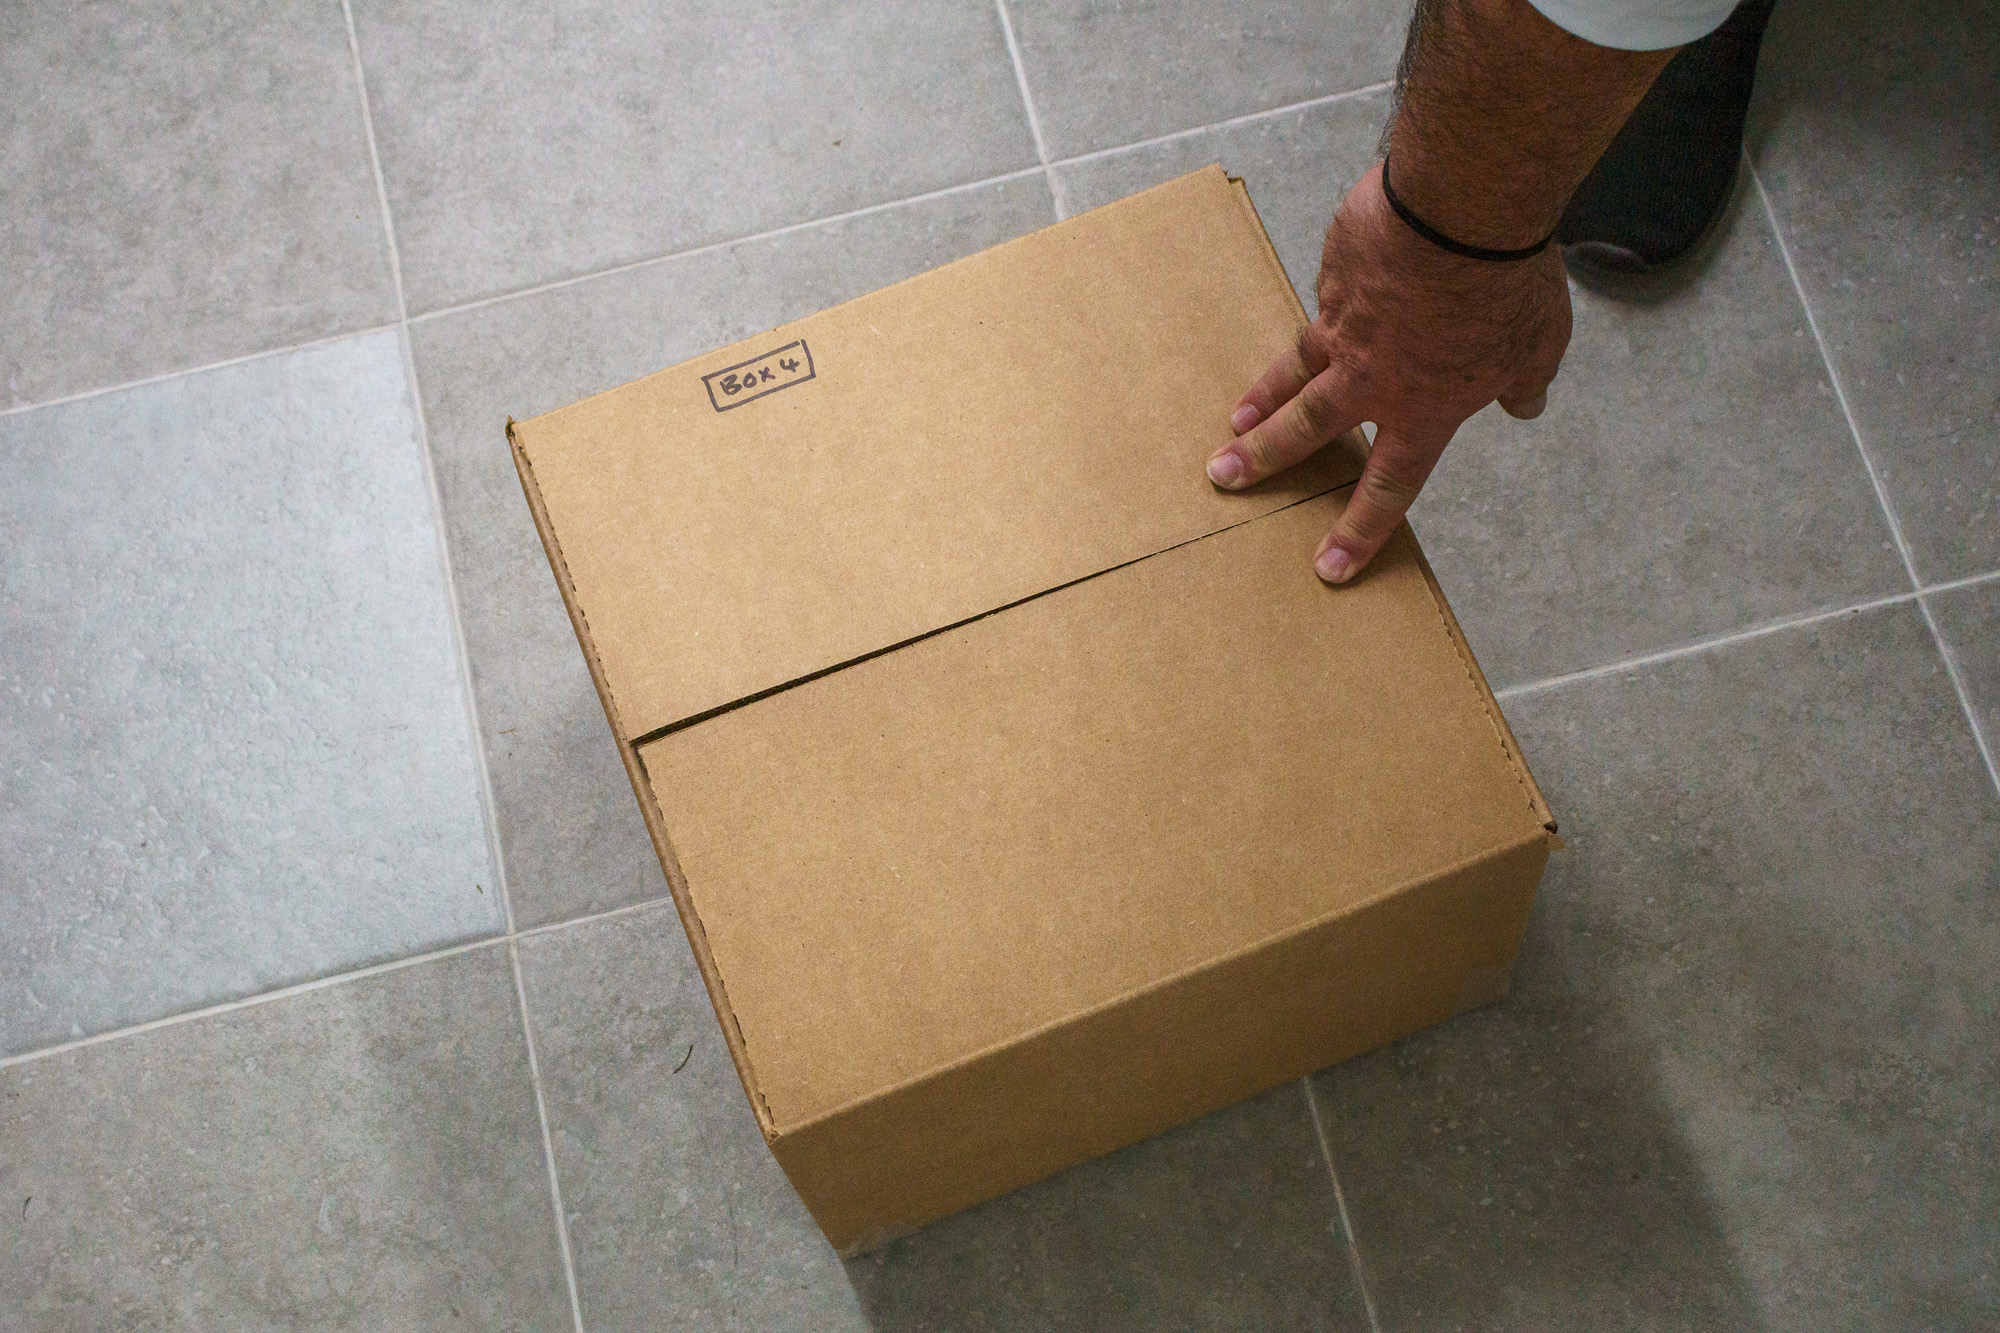
\includegraphics[width=0.60\linewidth]{figures/20201207T185905.jpg}
\end{center}
\caption{Box 4 and its contents.}
\label{figure:box-four}
\end{figure}

\subsection{Description}

Box 4 contains:

\begin{itemize}
    \item The two close-electronics power cables DR-CO-CE-PWCA and DR-CO-CE-PWCB.
\end{itemize}

The cables are wrapped onto the same drum. They are then packed in a cardboard box lined on all sides with 25~mm polystyrene foam sheets. See Figure~\ref{figure:box-four}.

Box 4 is $30 \times 30 \times 20$ cm ($L \times W \times H$) and has a weight of 4 kg.

\subsection{Unpacking Instructions}

There are no special unpacking instructions.

\subsection{Repacking Instructions}

There are no special repacking instructions.

%%%%%%%%%%%%%%%%%%%%%%%%%%%%%%%%%%%%%%%%%

\clearpage
\section{Box 5}

\begin{figure}
\begin{center}
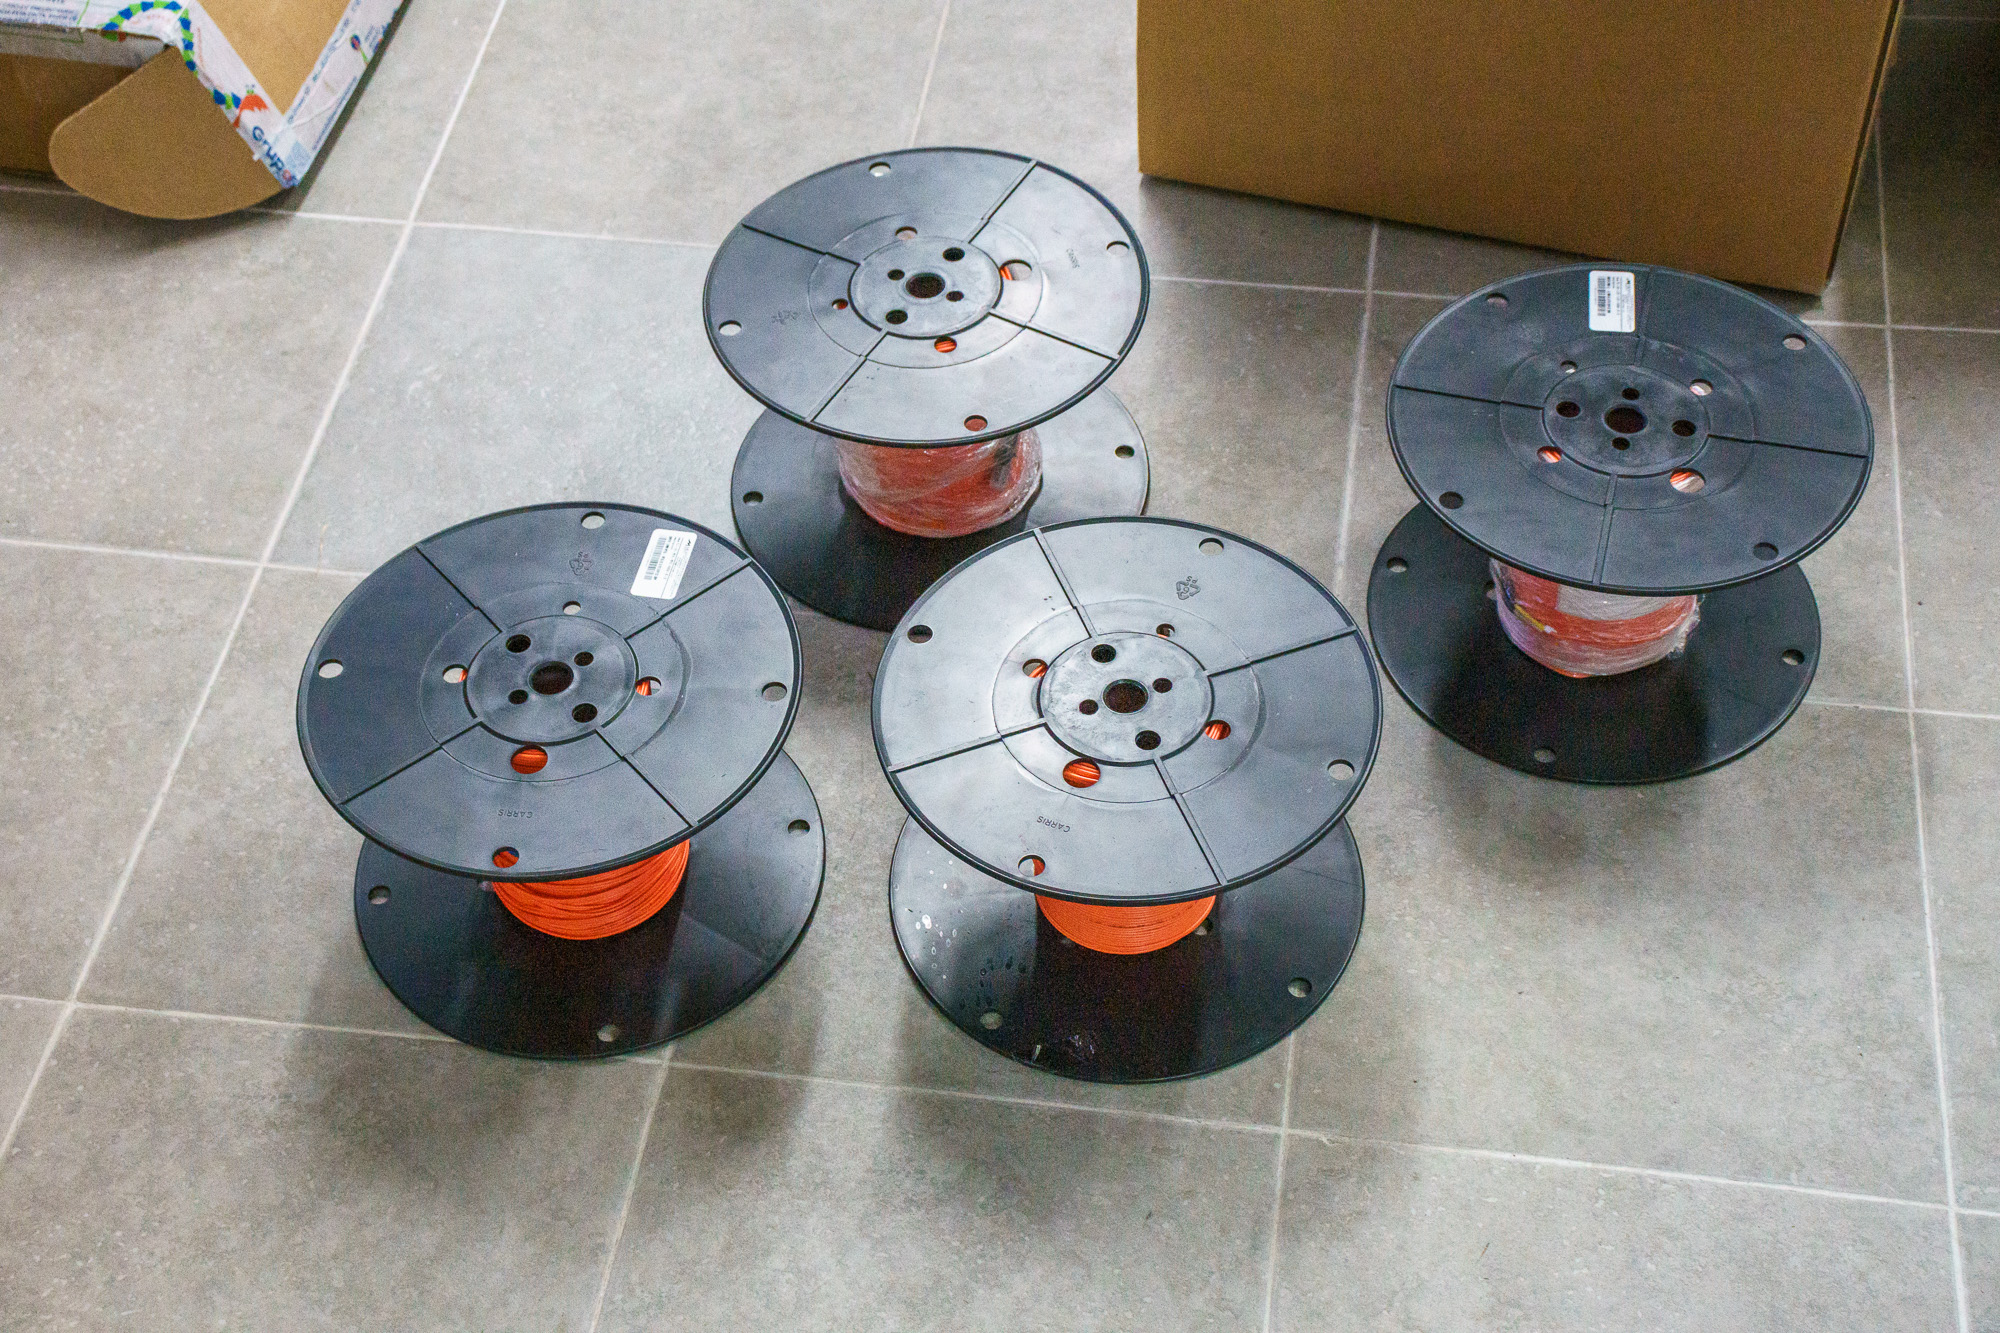
\includegraphics[width=0.60\linewidth]{figures/20201207T184739.jpg}\\[\smallskipamount]
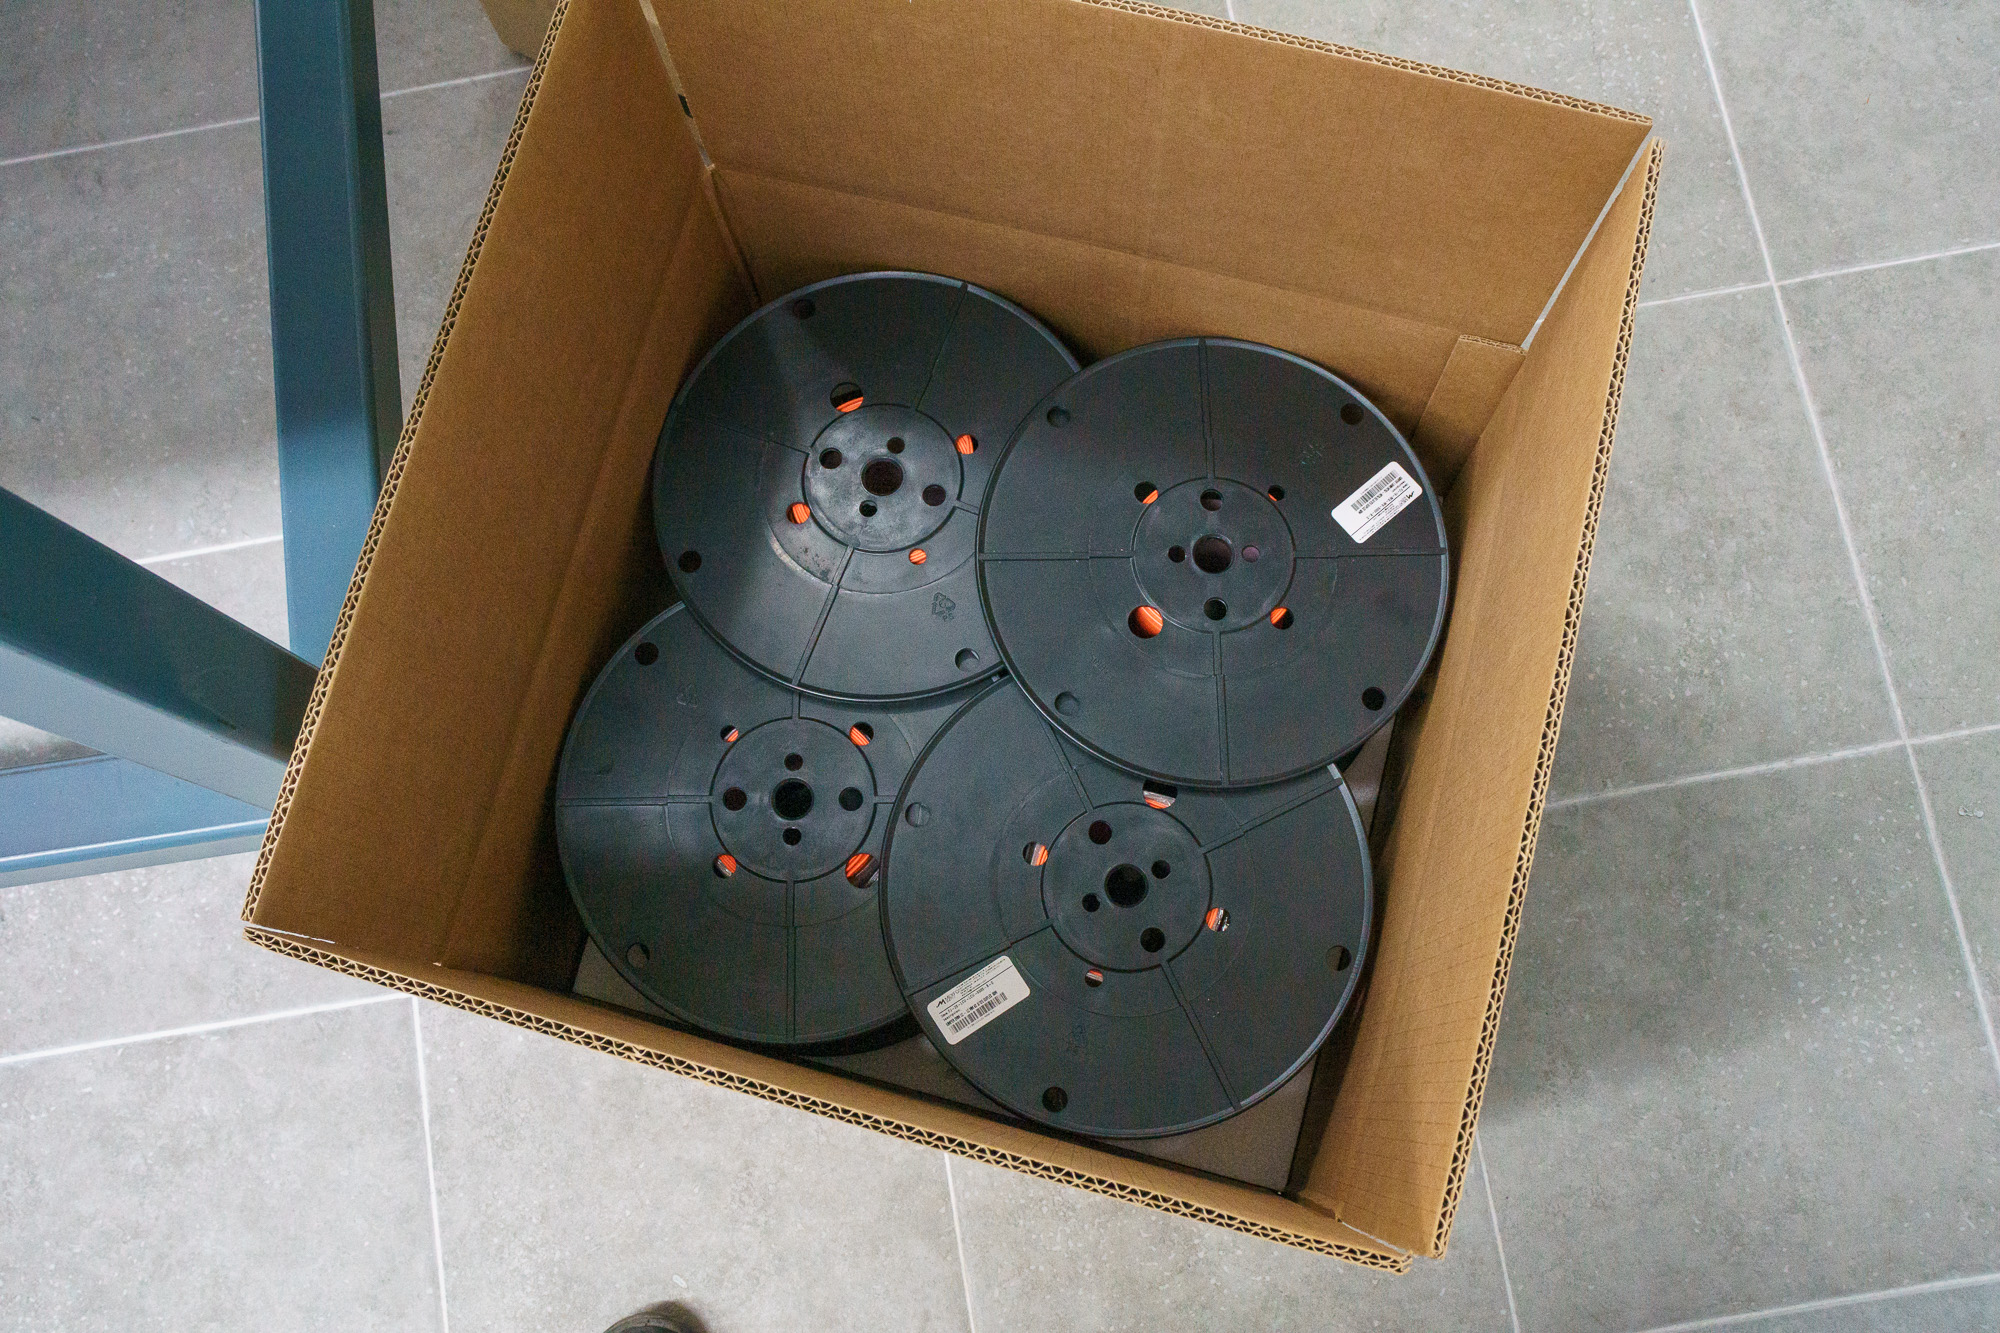
\includegraphics[width=0.60\linewidth]{figures/20201207T184823.jpg}\\[\smallskipamount]
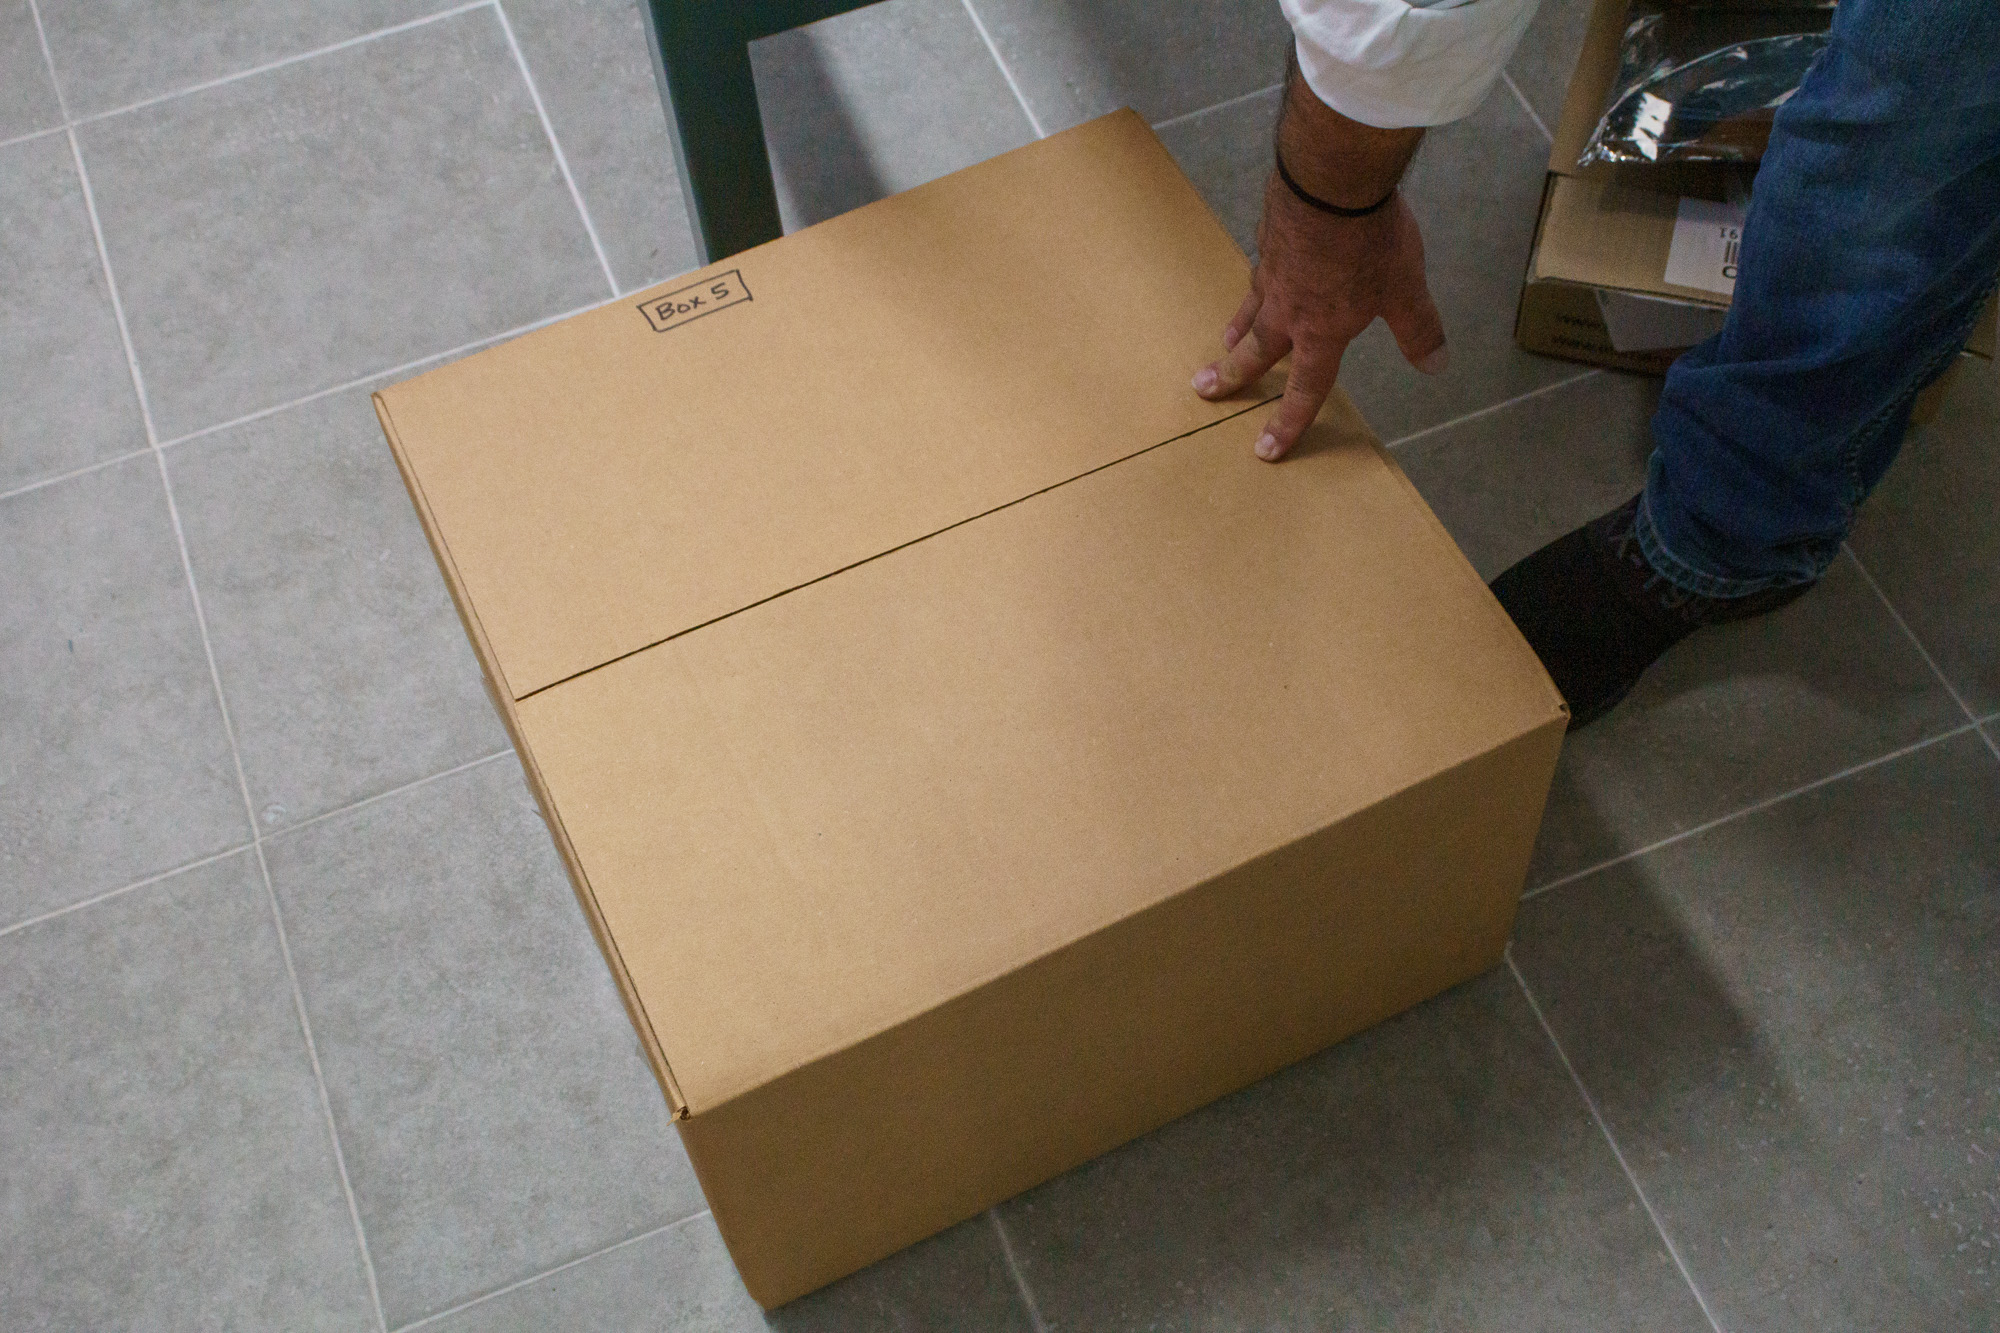
\includegraphics[width=0.60\linewidth]{figures/20201207T185114.jpg}
\end{center}
\caption{Box 5 and its contents.}
\label{figure:box-five}
\end{figure}

\subsection{Description}

Box 5 contains:

\begin{itemize}
    \item The two optical-fiber cables for the close electronics USB extender DR-CO-CE-USBREX-OFA and DR-CO-CE-USBREX-OFB.
\item The two optical-fiber cable for the blue detector DR-CO-BDH-OFA and DR-CO-BDH-OFB.
\end{itemize}

The cables are wrapped onto individual drums. They are then packed into a cardboard box lined on the top and bottom with 25~mm polystyrene foam sheets. See Figure~\ref{figure:box-five}.

Box 5 is  $45 \times 45 \times 25$~cm ($L \times W \times H$) and has a weight of 4 kg.

\subsection{Unpacking Instructions}

There are no special unpacking instructions.

\subsection{Repacking Instructions}

There are no special repacking instructions.

%%%%%%%%%%%%%%%%%%%%%%%%%%%%%%%%%%%%%%%%%

\clearpage
\section{Box 6}

\begin{figure}[bp]
\begin{center}
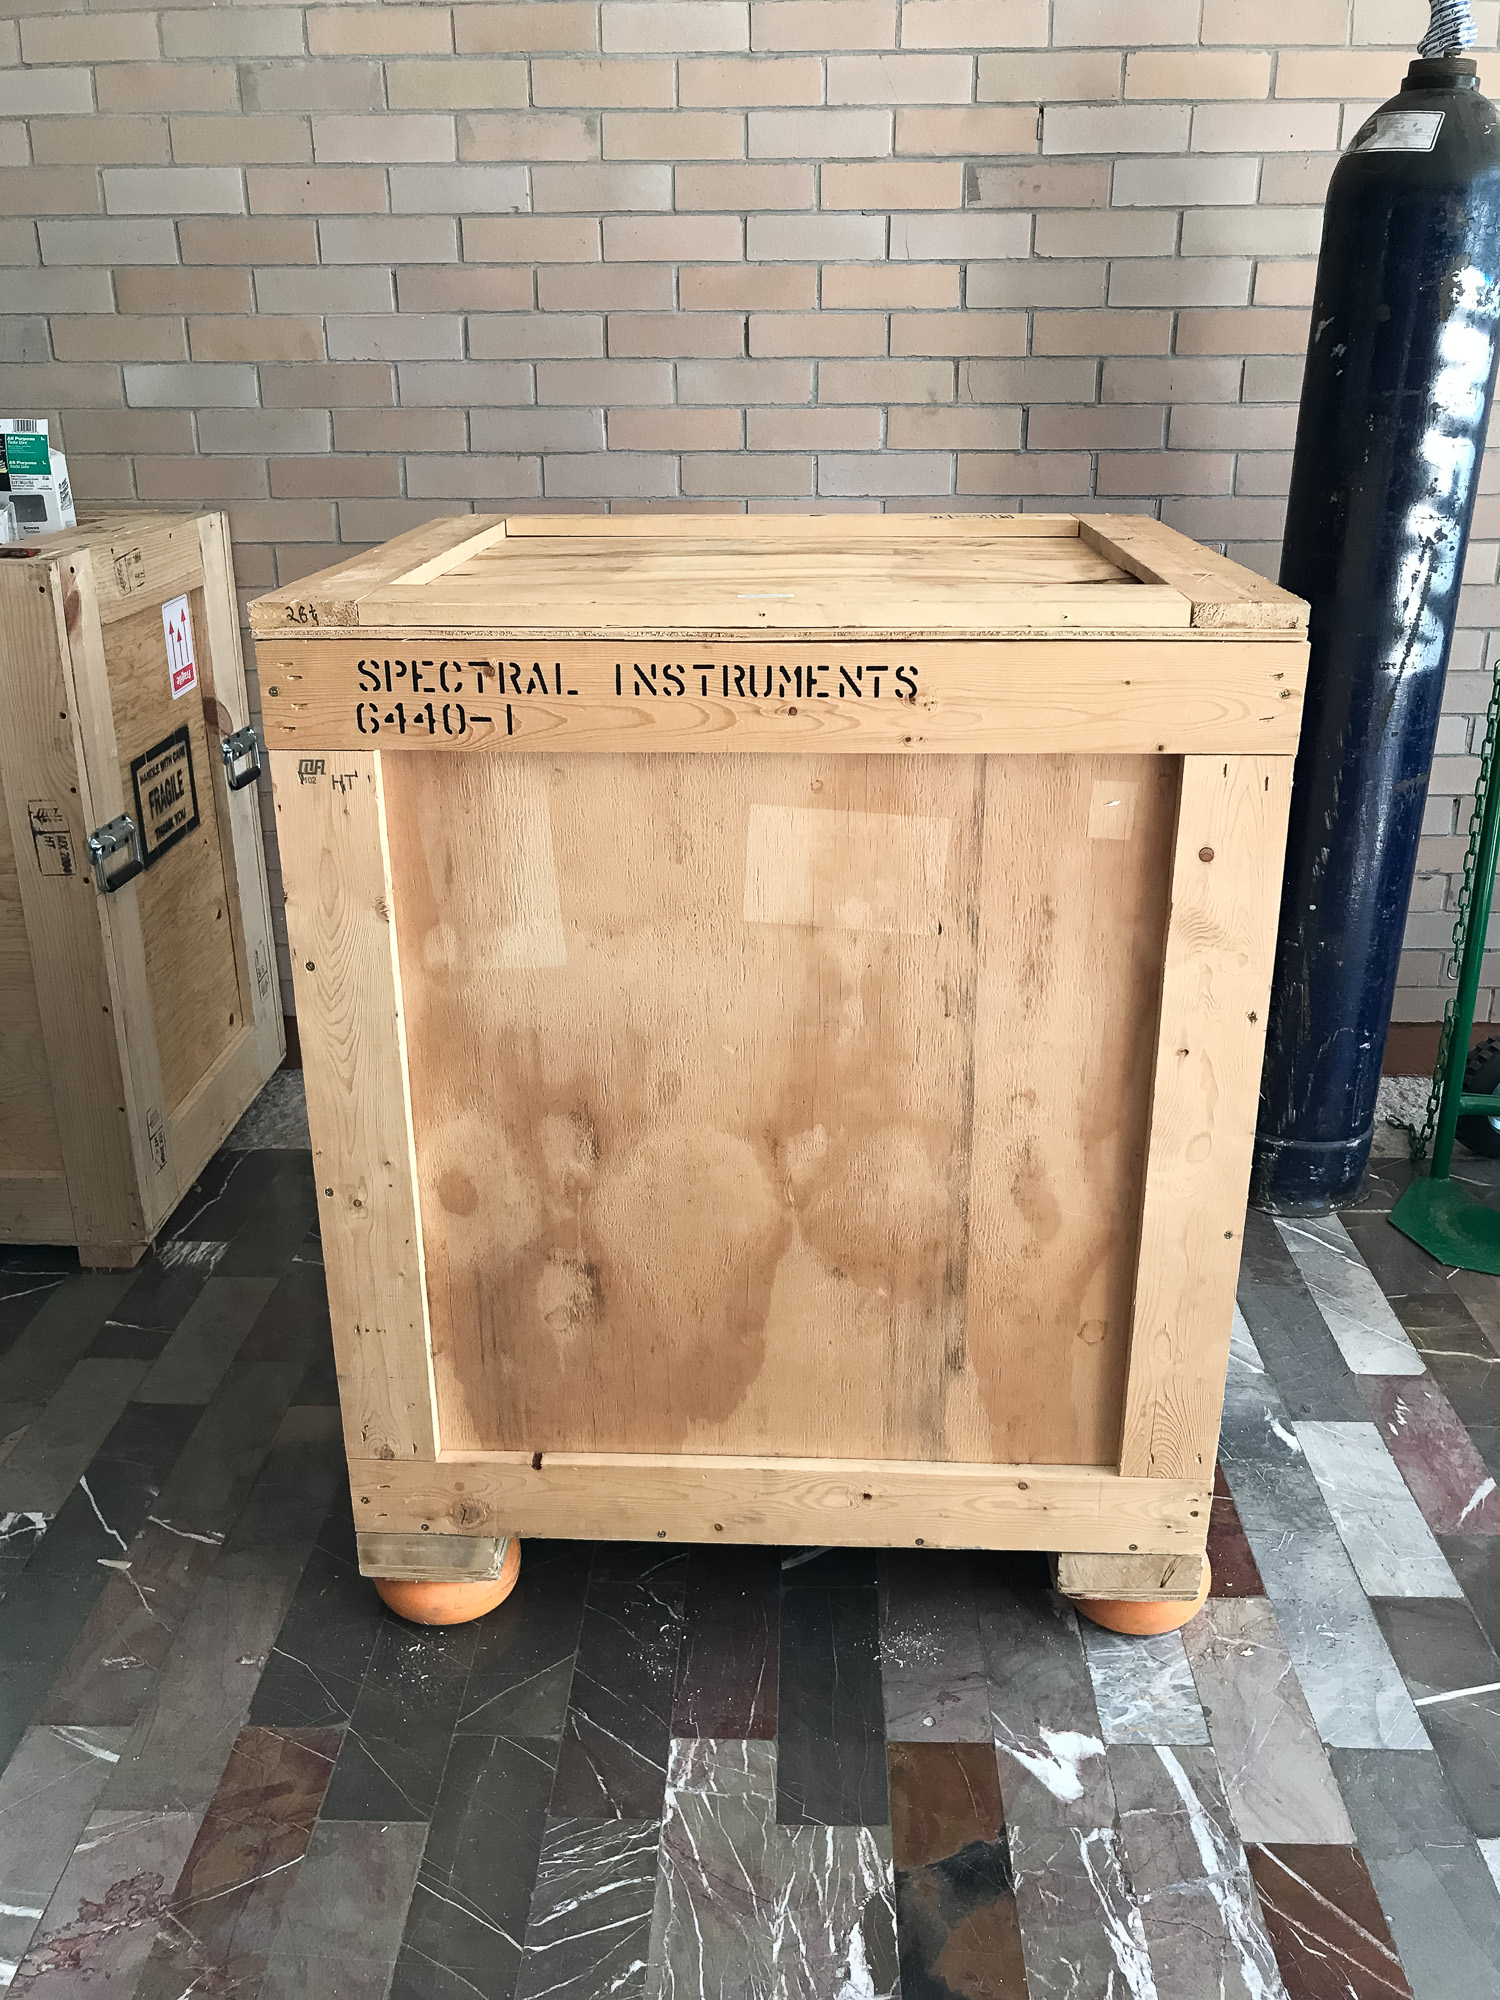
\includegraphics[width=0.45\linewidth]{figures/20210106T105641.jpg}
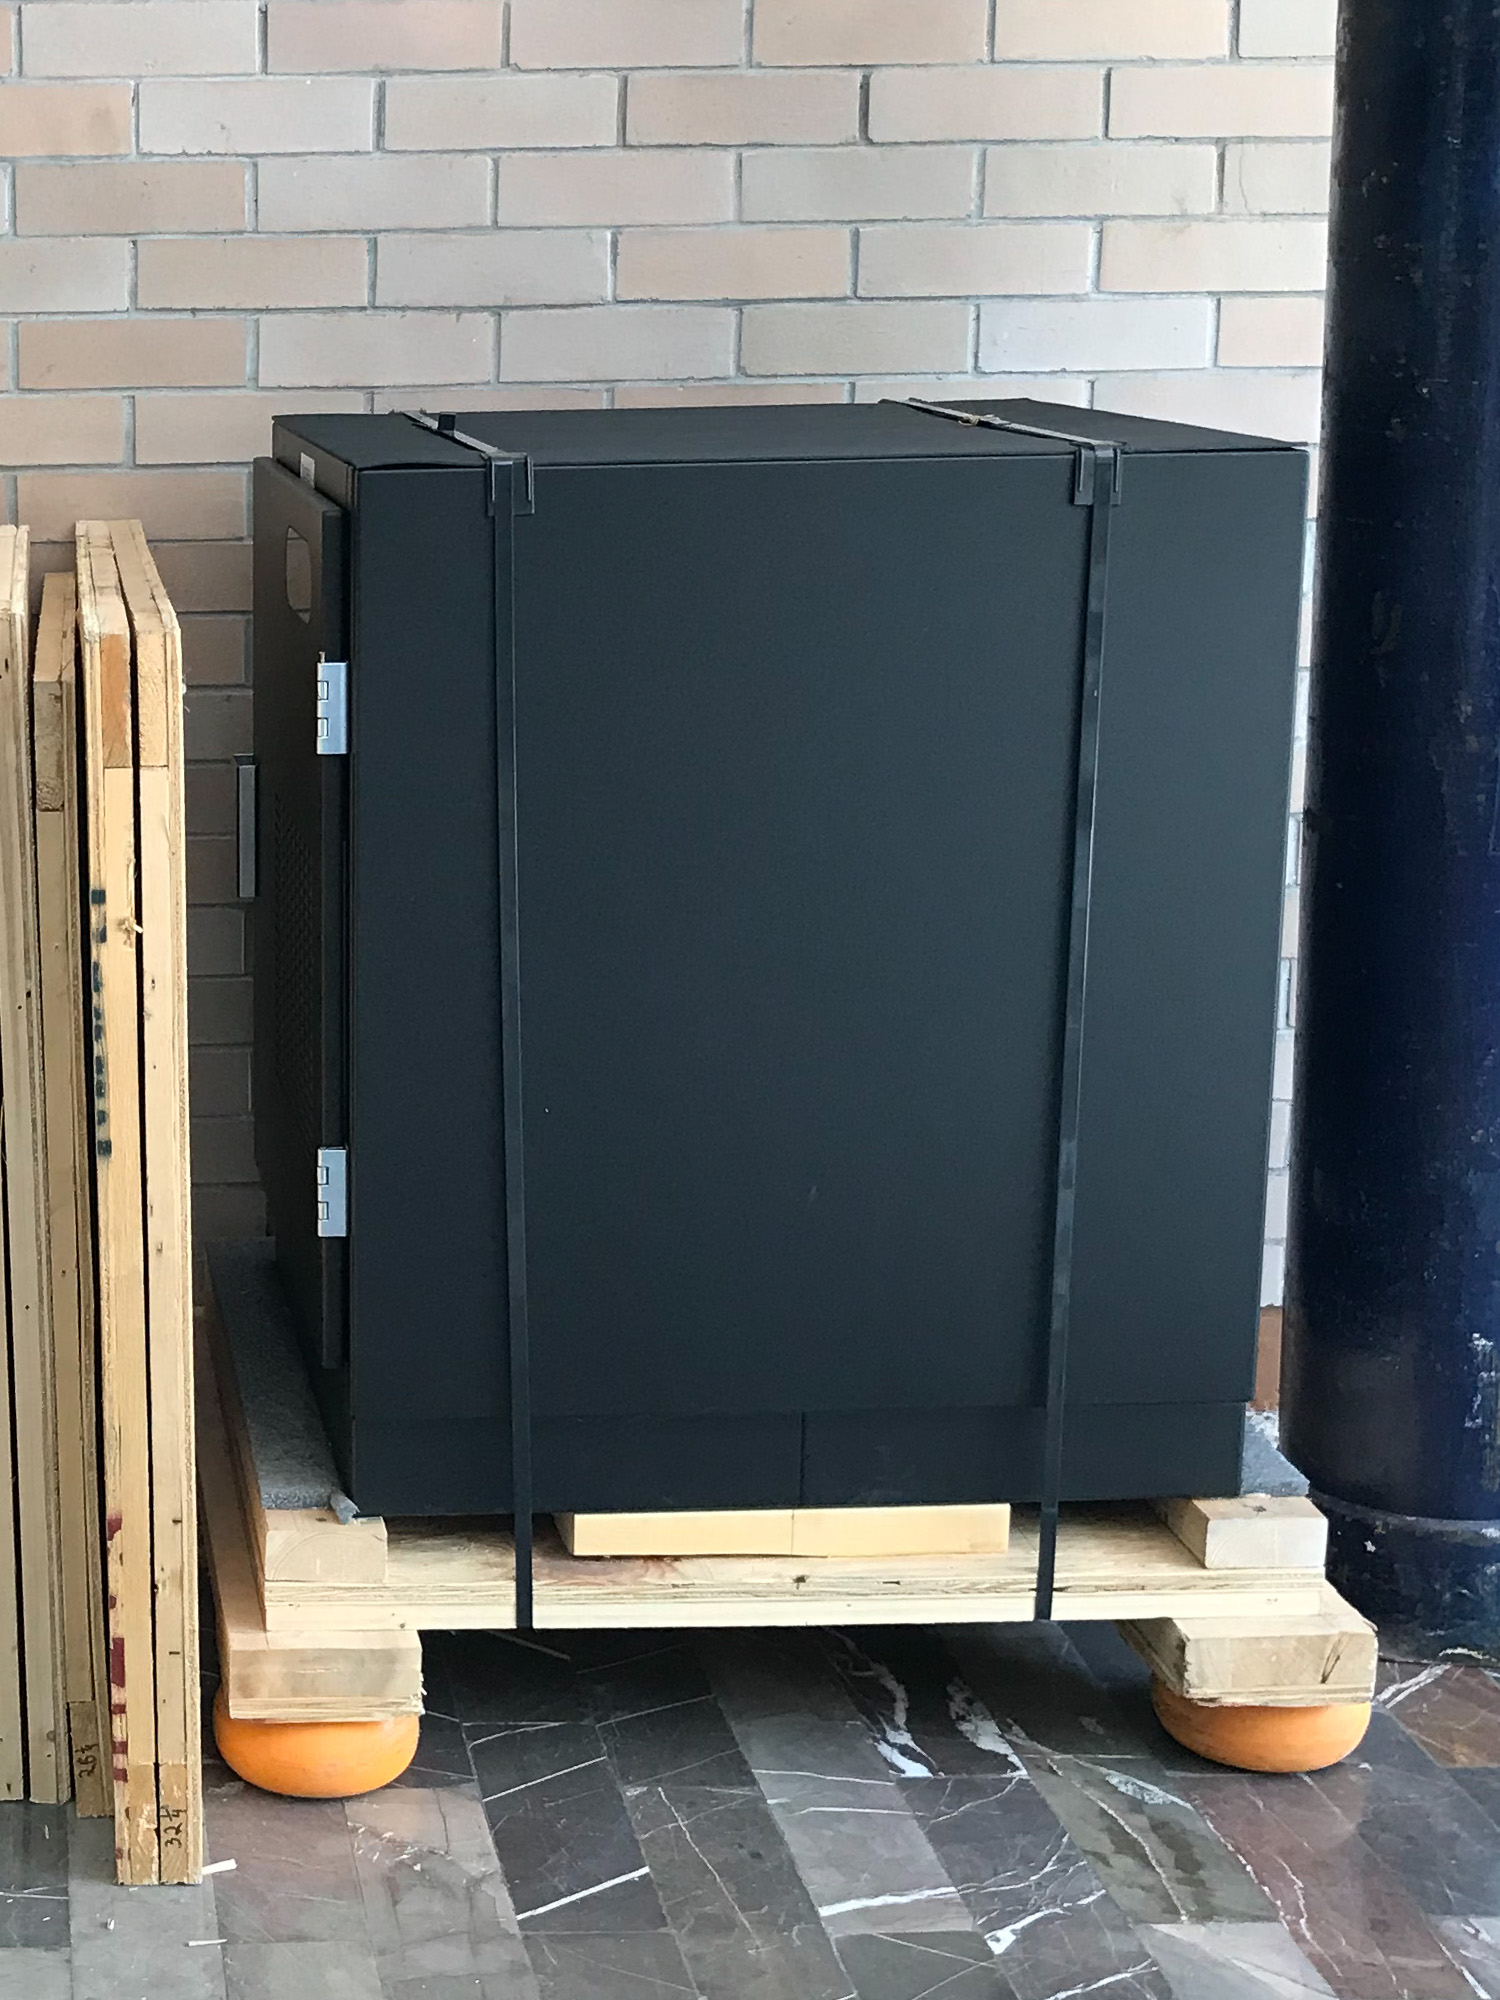
\includegraphics[width=0.45\linewidth]{figures/20201211T115036.jpg}
\end{center}
\caption{Box 6 and its contents.}
\label{figure:box-six}
\end{figure}

\begin{figure}[bp]
\begin{center}
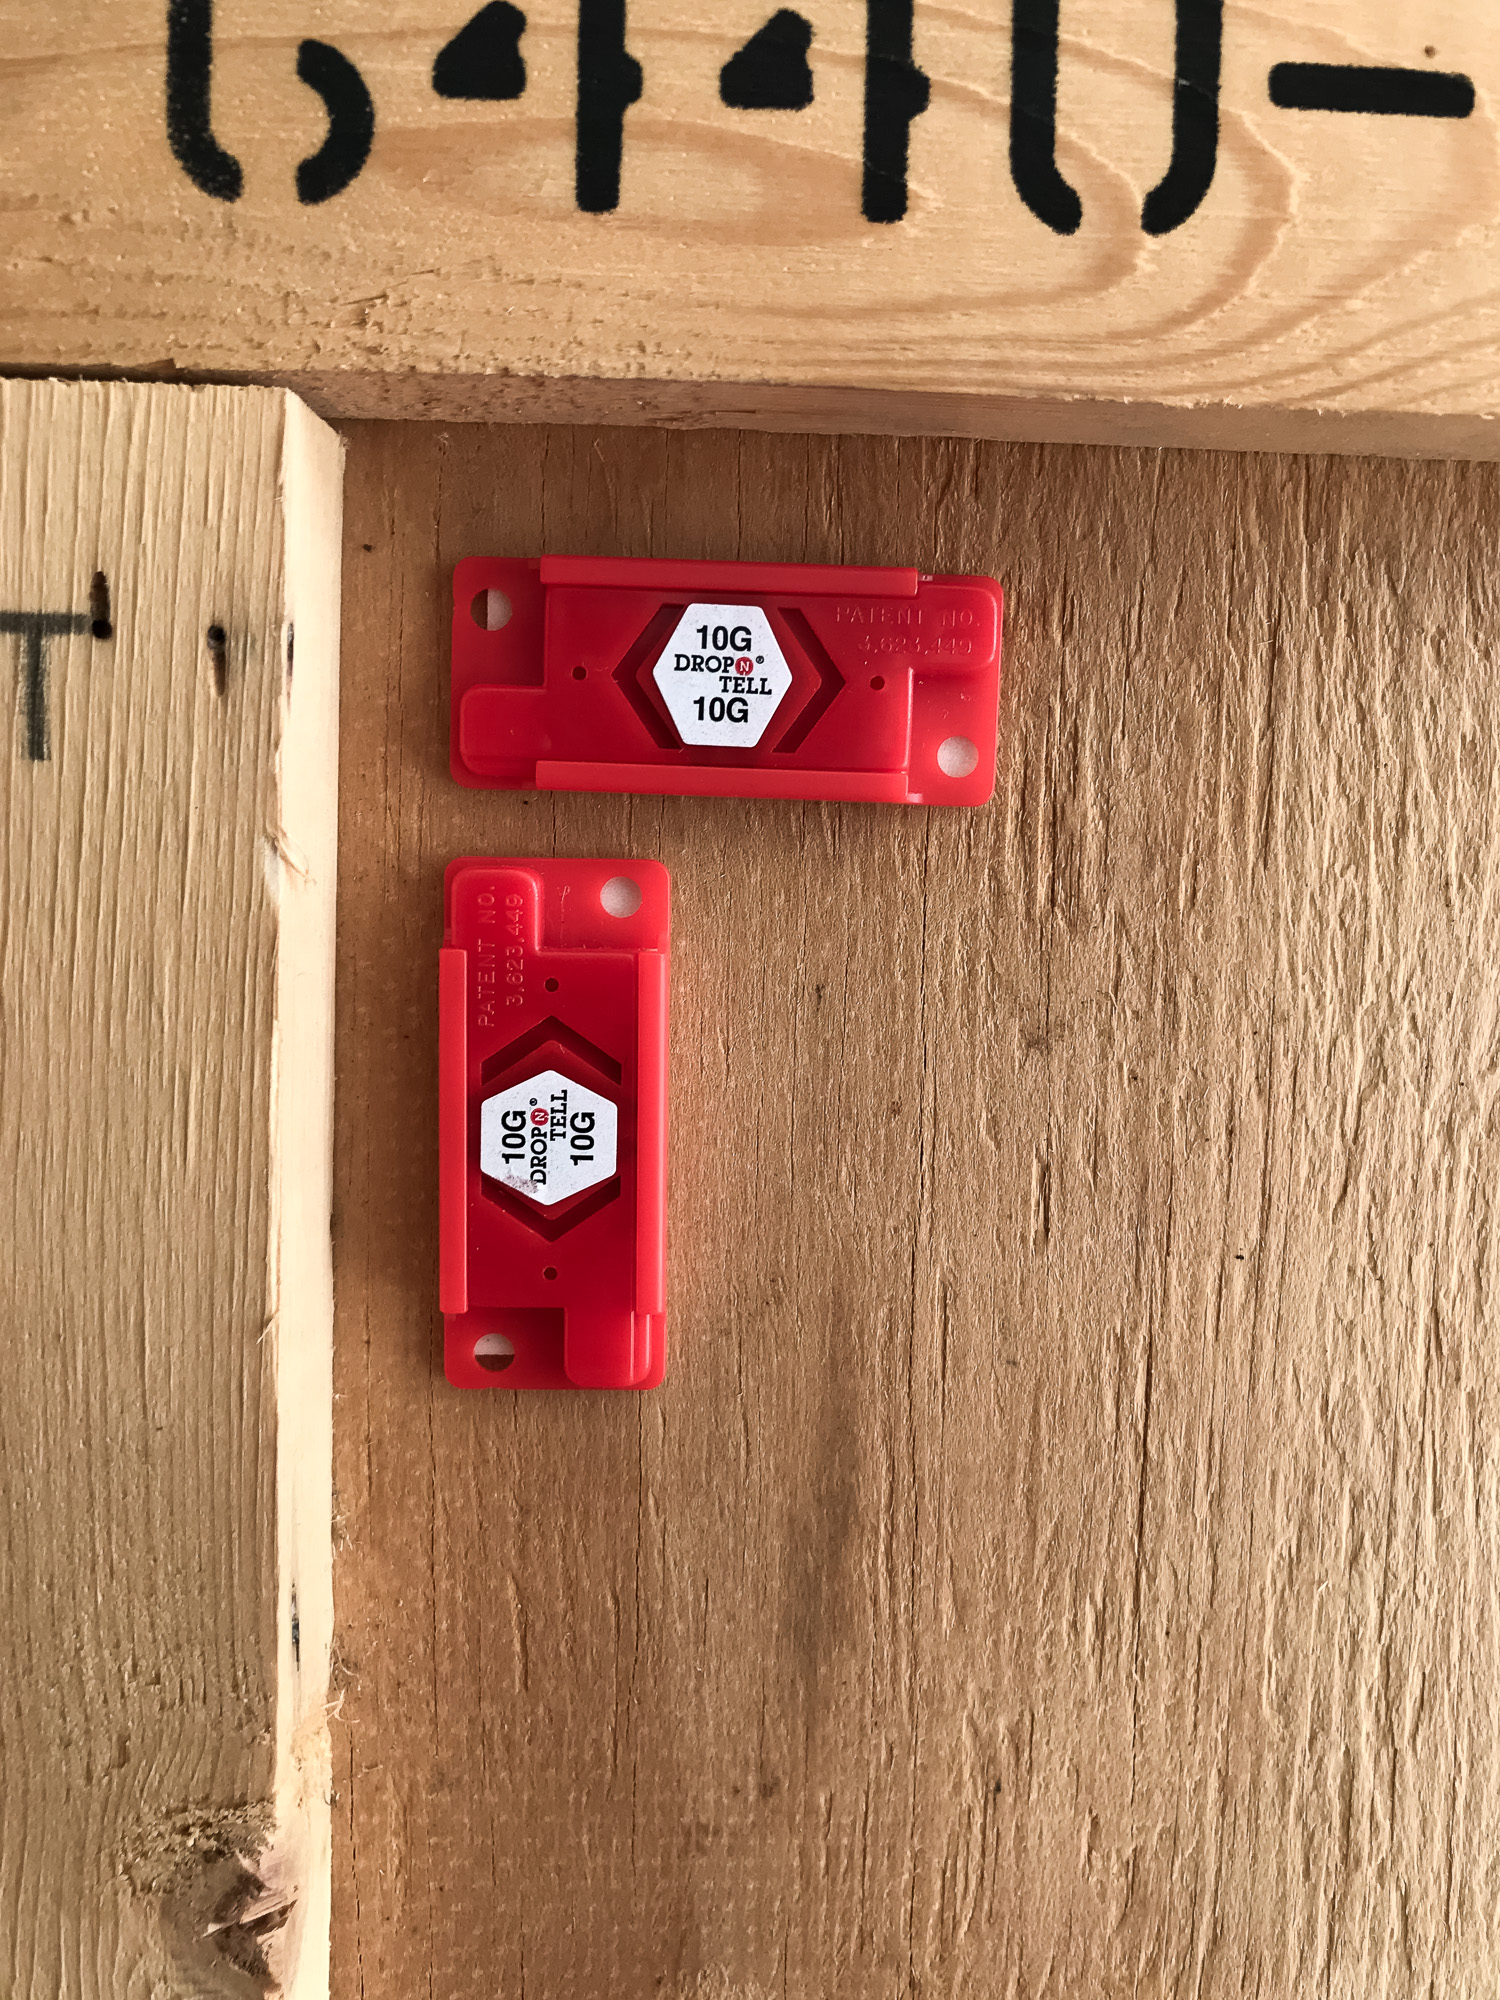
\includegraphics[width=0.3\linewidth]{figures/20210106T120810.jpg}
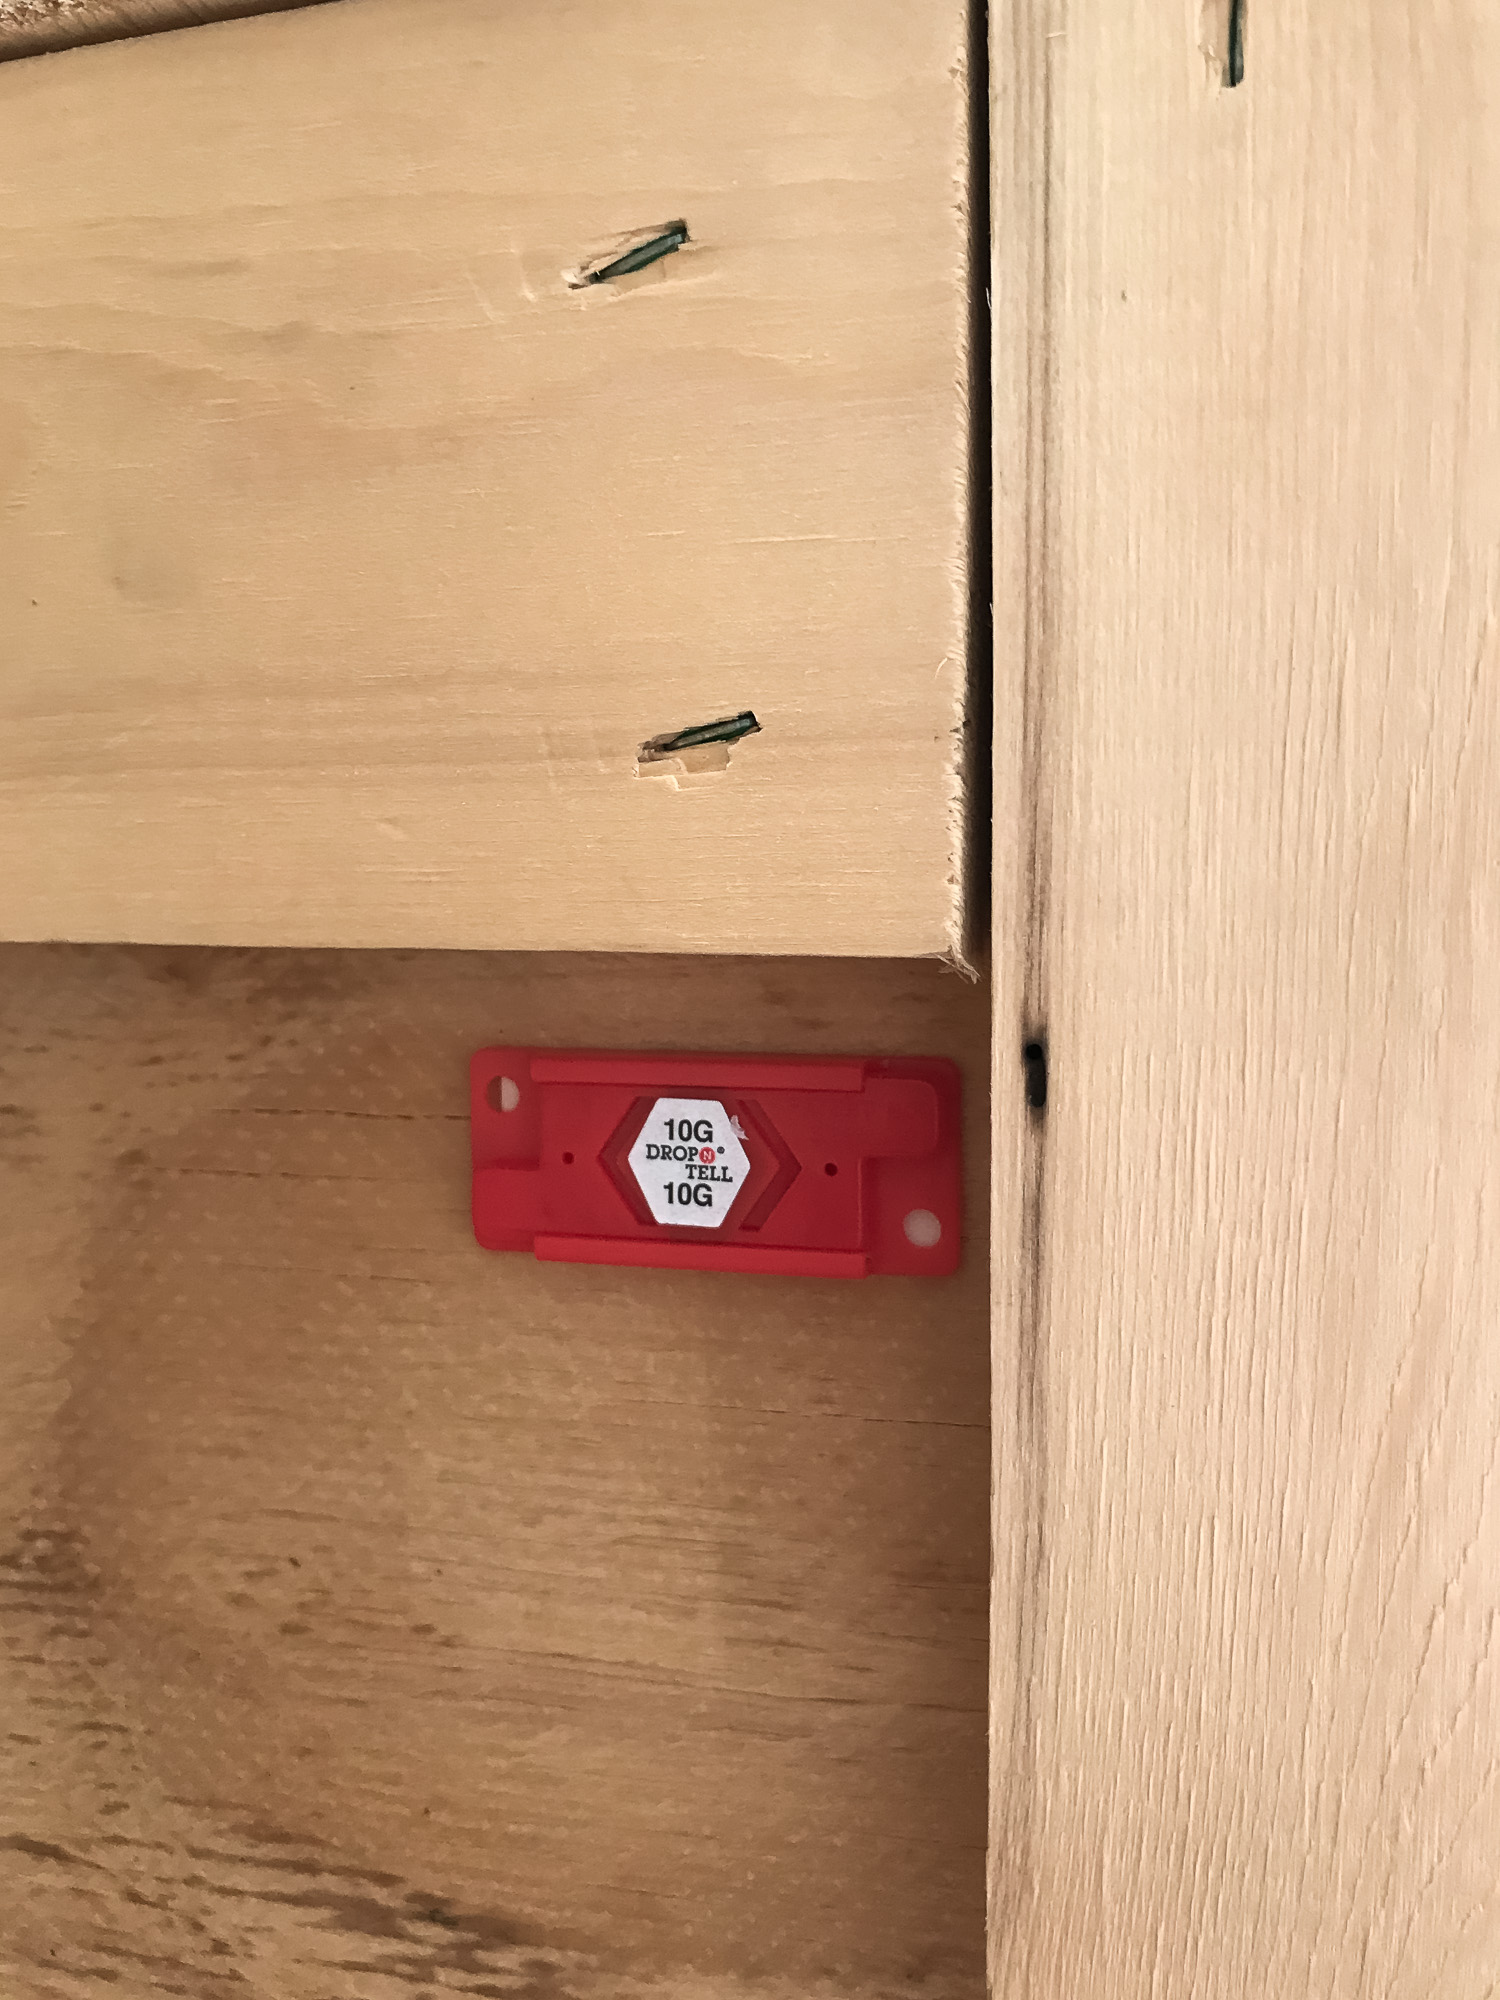
\includegraphics[width=0.3\linewidth]{figures/20210106T120814.jpg}
\end{center}
\caption{Box 6 external sensors. Left: two of the 10$g$ sensors. Right: the other two 10$g$ sensor.}
\label{figure:box-six-external-sensors}
\end{figure}

\subsection{Description}

Box 6 contains:

\begin{itemize}
    \item The blue detector service cabinet DR-CO-CR-BDSC.
    \item The 1-wire sensors  DR-CO-CR-ES3 and DR-CO-CR-ES4 and the 1-wire cable DR-CO-CR-ES4-OWC, installed in the service cabinet.
\end{itemize}

See Figure~\ref{figure:box-six}.

The box has three 10-g impact indicators on the outside (see Figure~\ref{figure:box-six-external-sensors})

Box 6 is  $82 \times 62 \times 102$~cm ($L \times W \times H$) and has a weight of 157 kg.

\subsection{Unpacking Instructions}

\begin{enumerate}
\item Box 6 and the cabinet it contains should not be tilted by more than 50 degrees from vertical. If the cabinet angle ever exceeds 50 degrees from vertical it must be allowed to sit idle for 4 hours before operating.
\item Verify that the external 10-g impact indicators are not activated. If they are, consult with the UNAM team before proceeding further.
\item Remove the screws that fasten the lid of the box. Remove the lid.
\item Remove the screws that fasten the sides of the box together and to the base. Remove the sides.
\item Leave the cabinet on the base of the box. Do not remove the metal straps.
\item Store the screws and the box sides and top in a safe place.
\end{enumerate}

\subsection{Repacking Instructions}

\begin{enumerate}
\item Verify that the external 10-g indicators are not activated. If they are, replace them with spares from Box 28.
\item Replace the sides of the box, using the screws to attach them together and to the base.
\item Replace the top of the box, using the crews to attach it to the sides.
\end{enumerate}

%%%%%%%%%%%%%%%%%%%%%%%%%%%%%%%%%%%%%%%%%

\clearpage
\section{Box 7}

\begin{figure}[bp]
\begin{center}
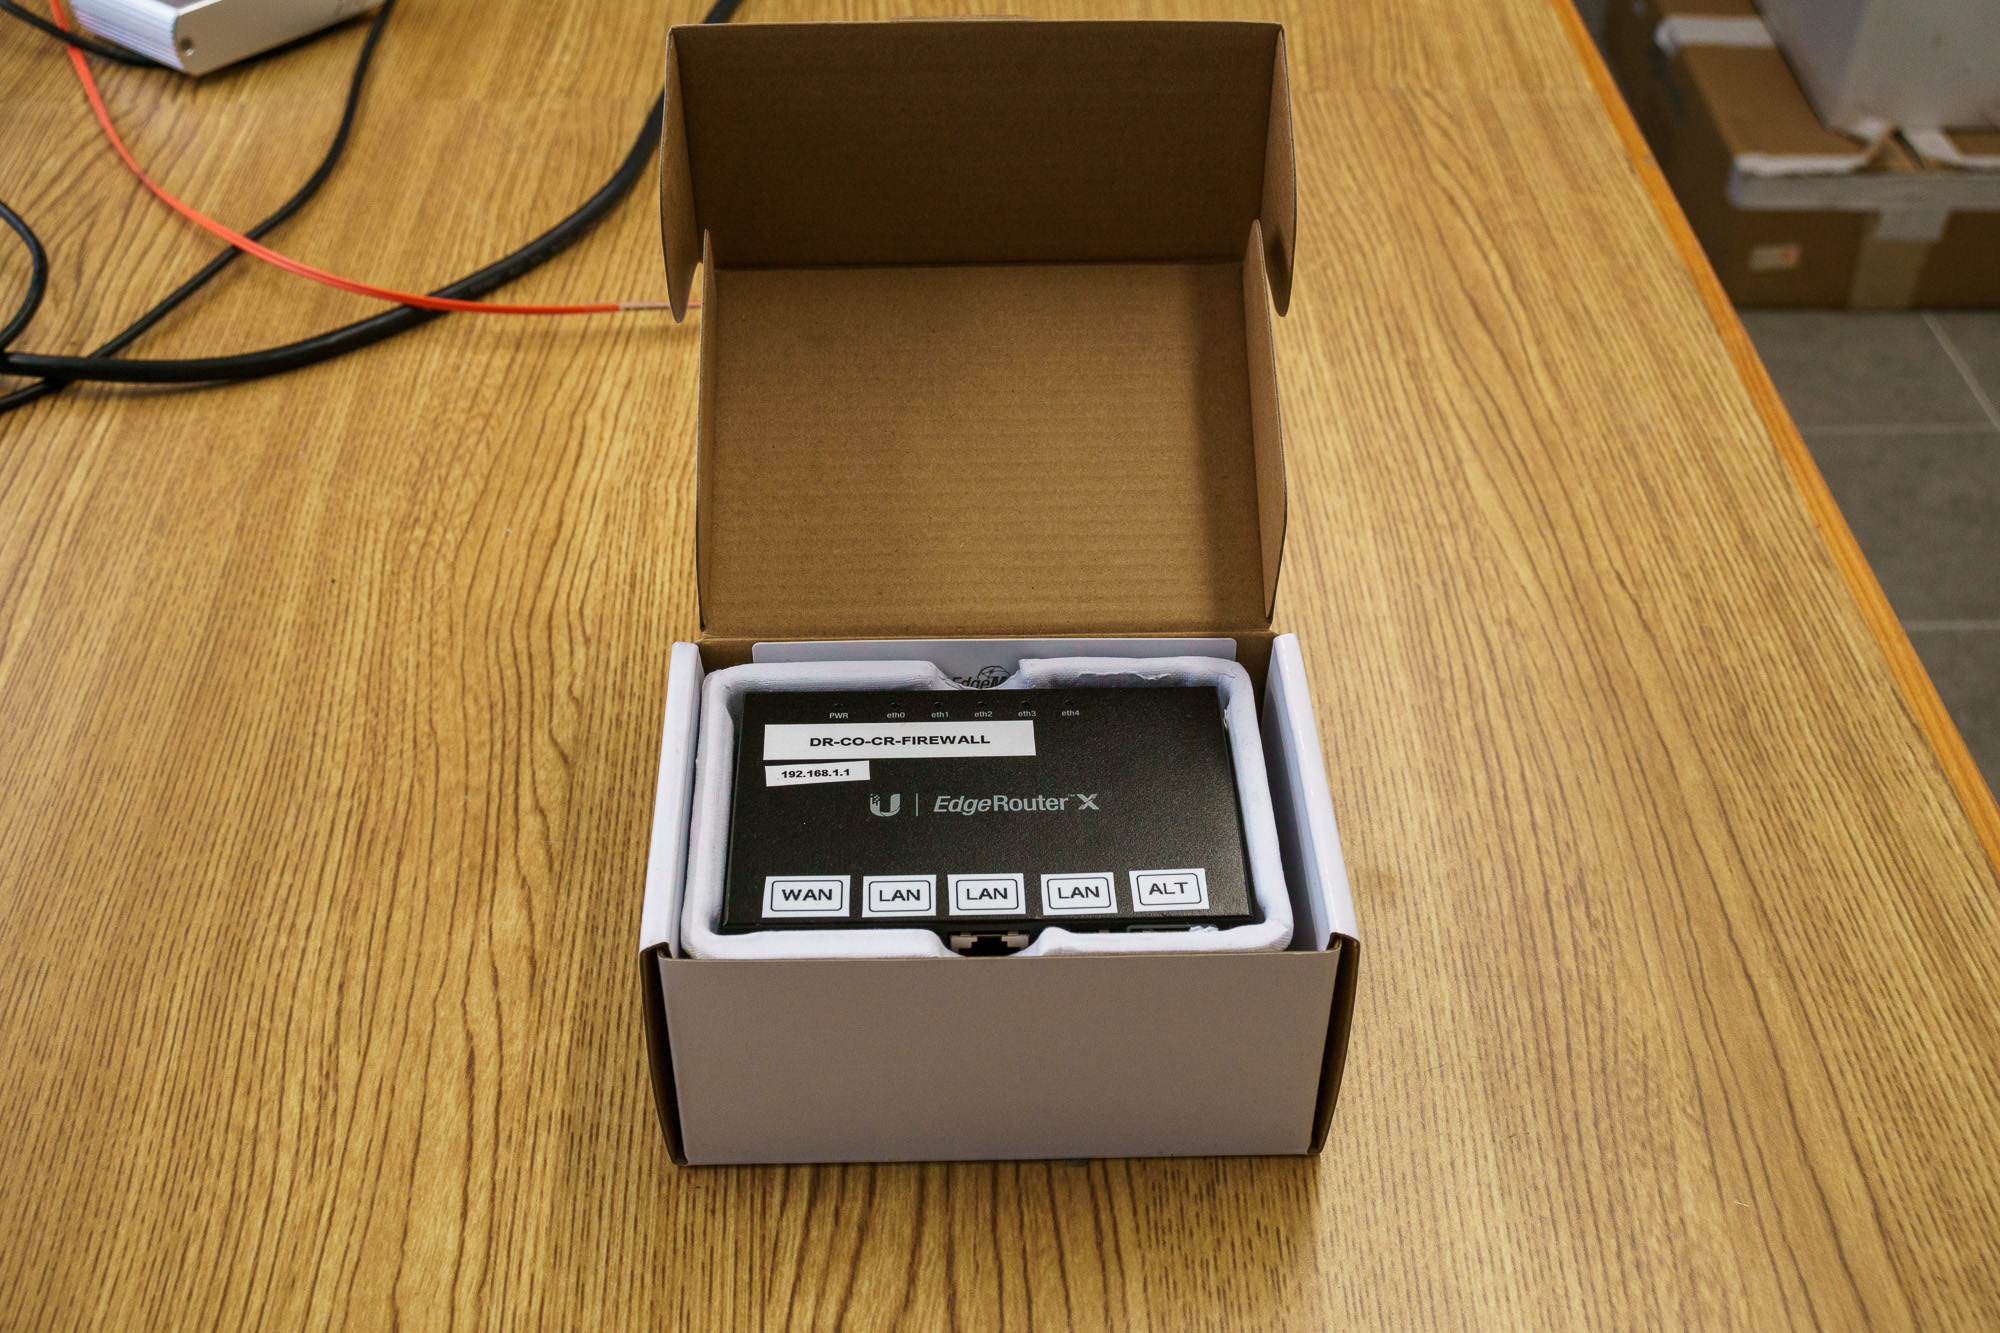
\includegraphics[width=0.45\linewidth]{figures/20201207T170111.jpg} 
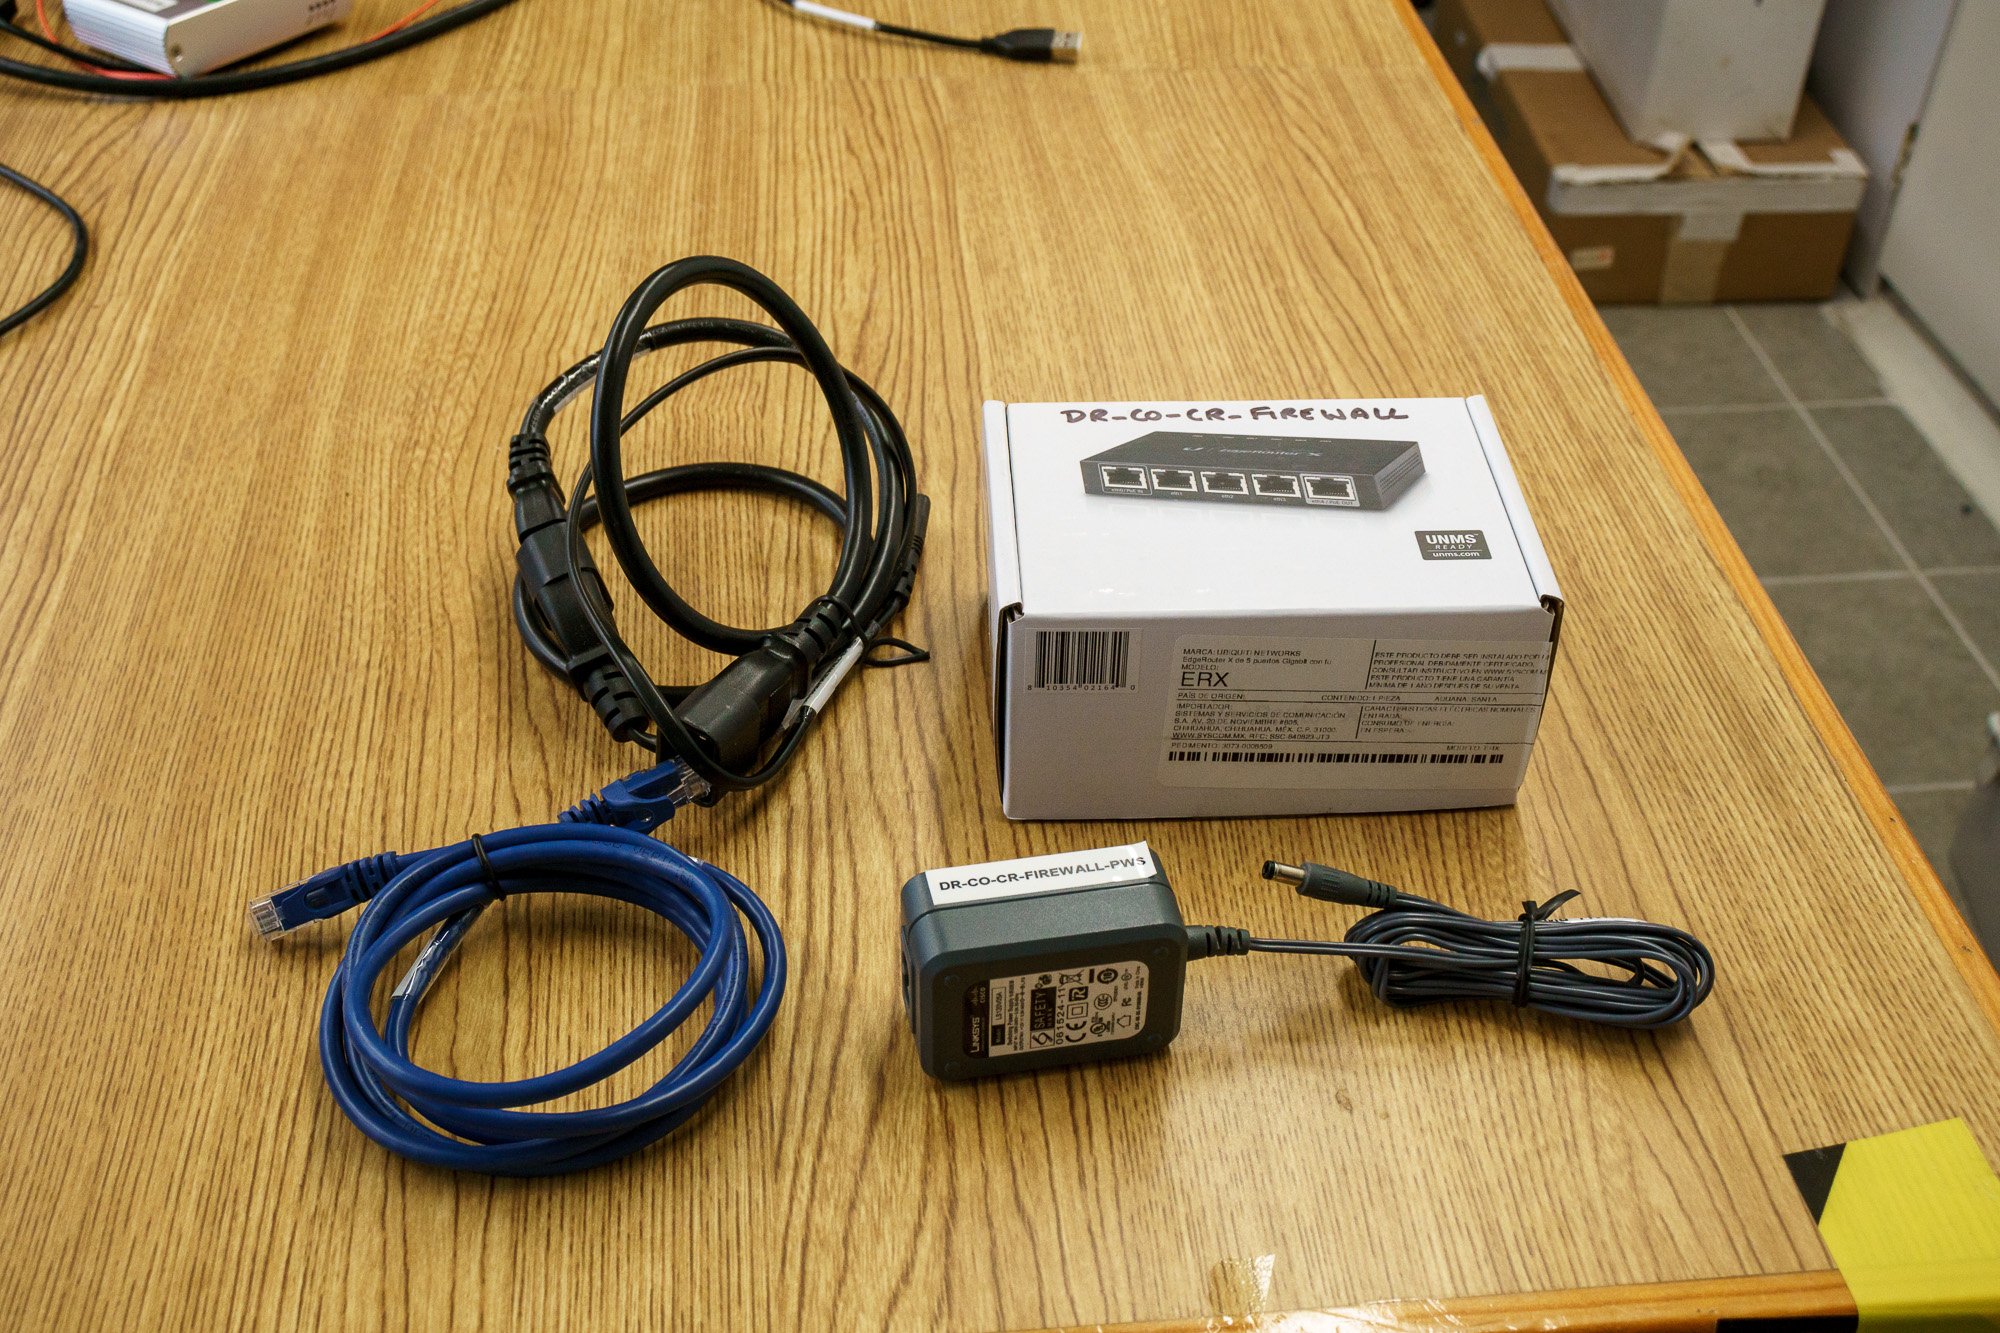
\includegraphics[width=0.45\linewidth]{figures/20201207T170134.jpg}\\[\smallskipamount]
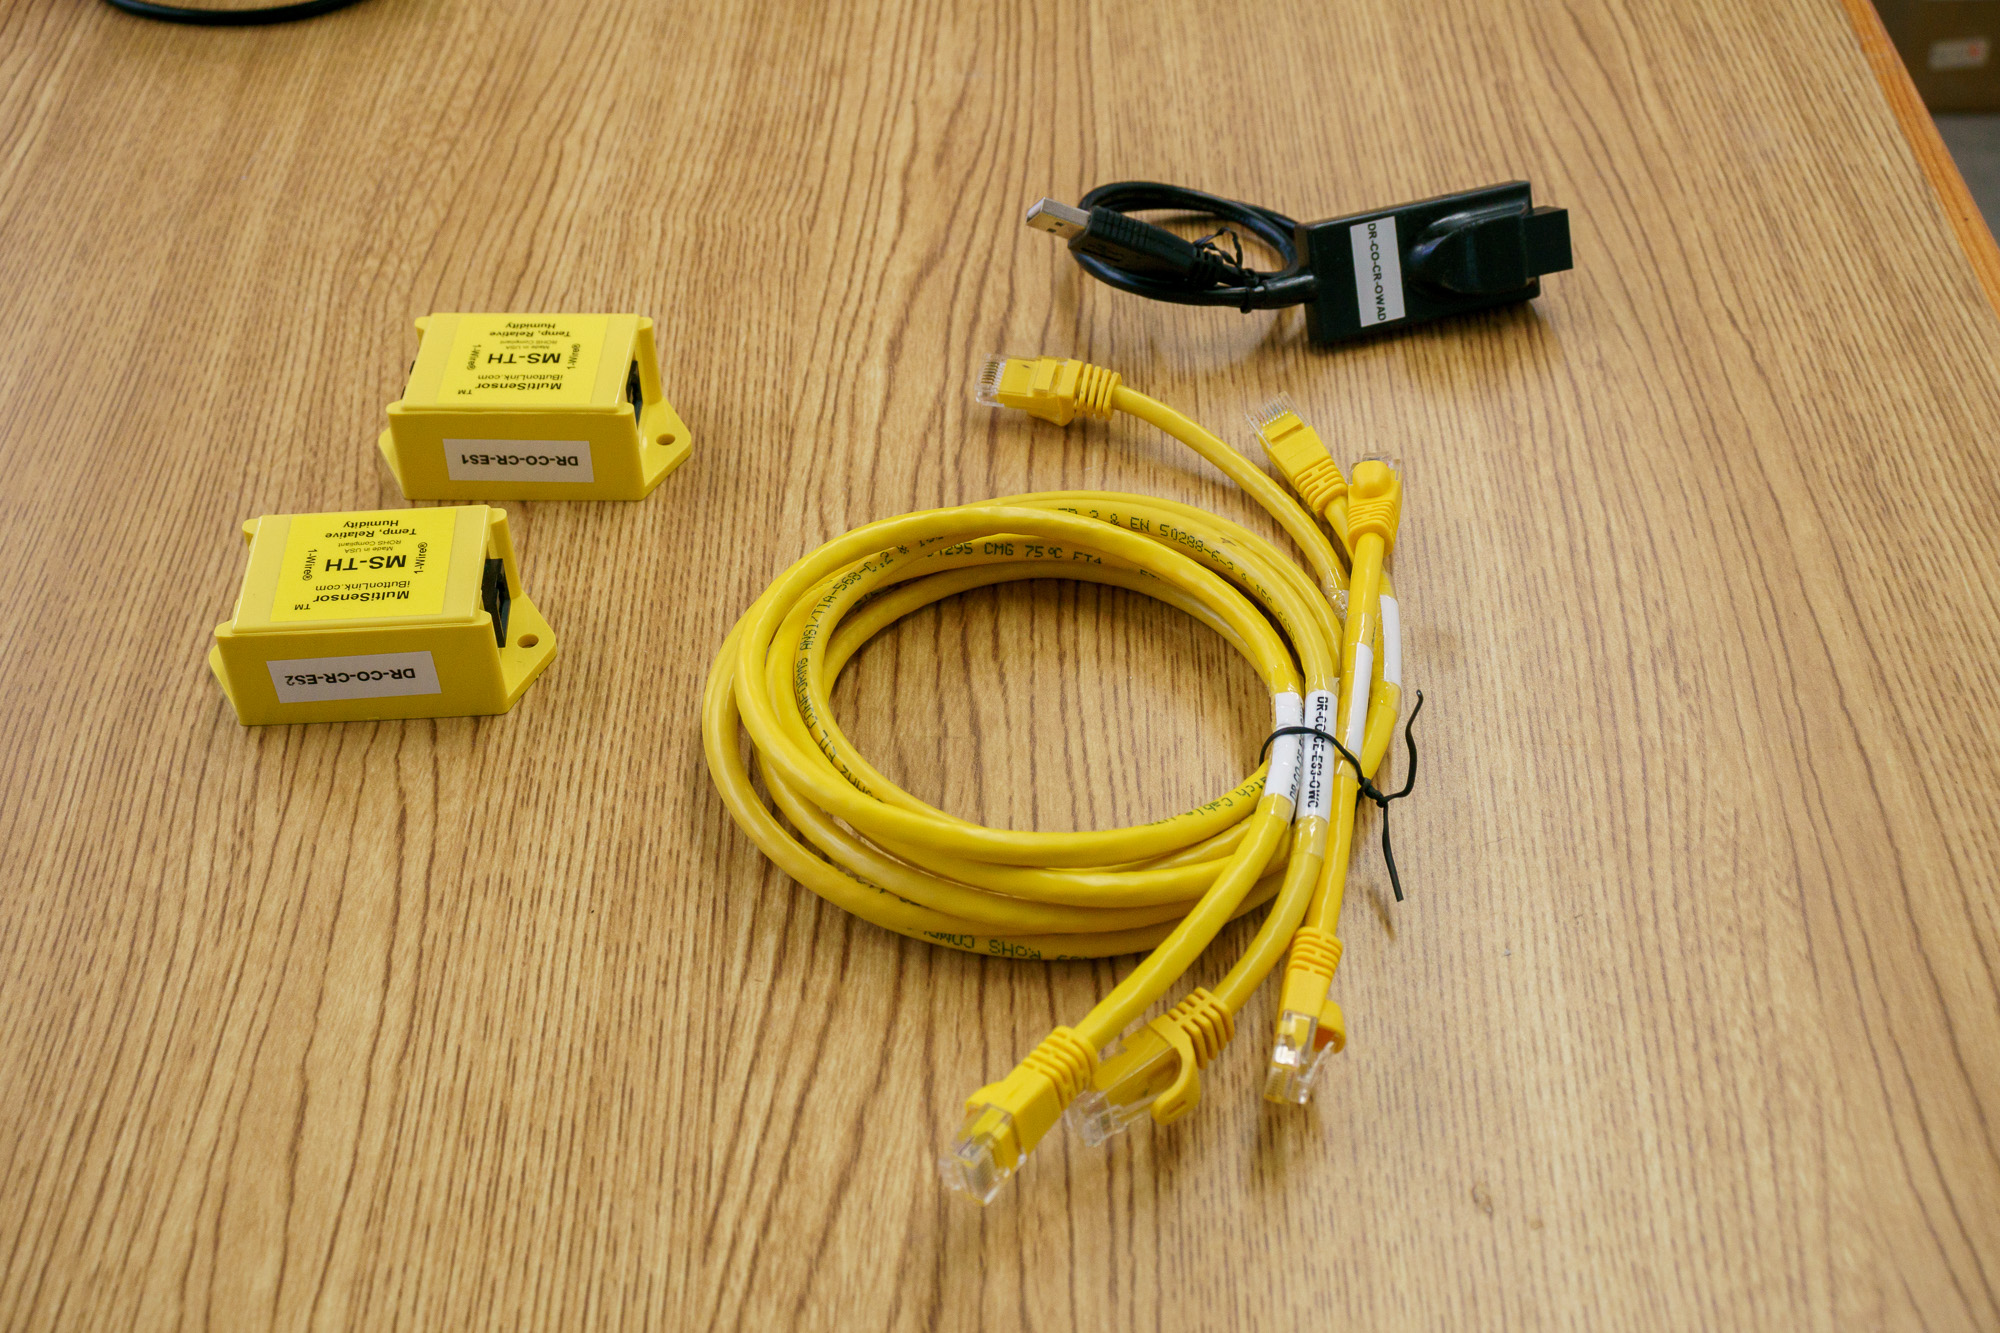
\includegraphics[width=0.45\linewidth]{figures/20201207T171428.jpg} 
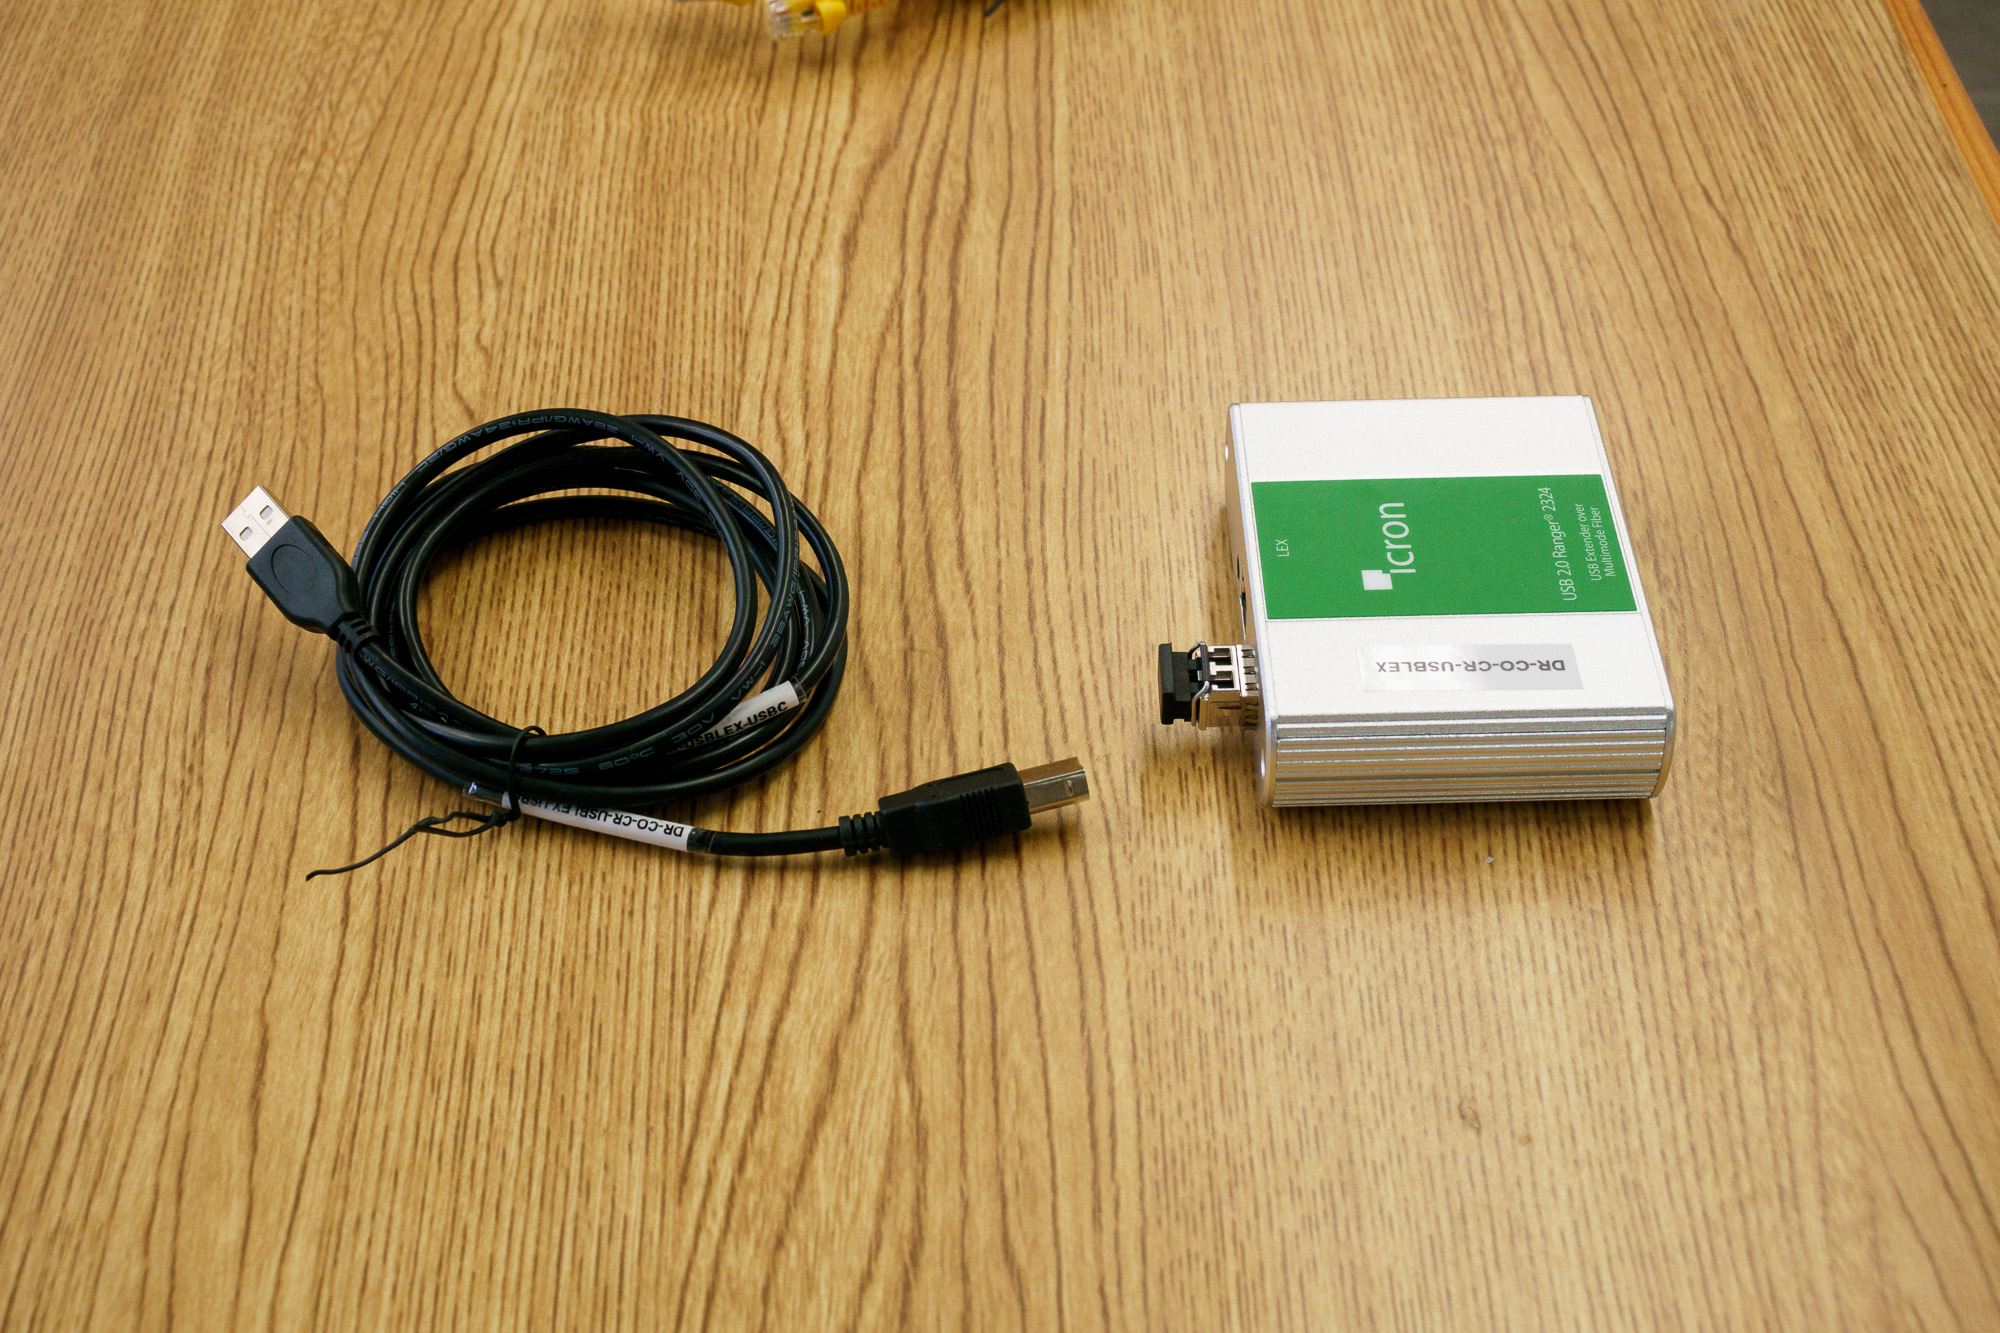
\includegraphics[width=0.45\linewidth]{figures/20201207T171439.jpg}\\[\smallskipamount]
\end{center}
\caption{Box 7 and its contents. Upper left: The firewall DR-CO-CR-FIREWALL in its box. Upper right: The firewall DR-CO-CR-FIREWALL, its power supply DR-CO-CR-FIREWALL-PS, power cable DR-CO-CR-FIREWALL-PWC, extension power cable,
DR-CO-CR-FIREWALL-EPWC, and Ethernet cable
DR-CO-CR-FIREWALL-ETHC. Lower left:  The 1-wire adapter DR-CO-CR-OWAD, 
the two 1-wire sensors for the control room rack 
DR-CO-CR-ES1 and
DR-CO-CR-ES2
along with the three yellow 1-wire cables 
DR-CO-CR-ES1-OWC,
DR-CO-CR-ES2-OWC, and
DR-CO-CR-ES3-OWC. Lower right:  The USB extender LEX 
DR-CO-CR-USBLEX and its USB cable
DR-CO-CR-USBLEX-USBC.}
\label{figure:box-seven-a}
\end{figure}

\begin{figure}[bp]
\begin{center}
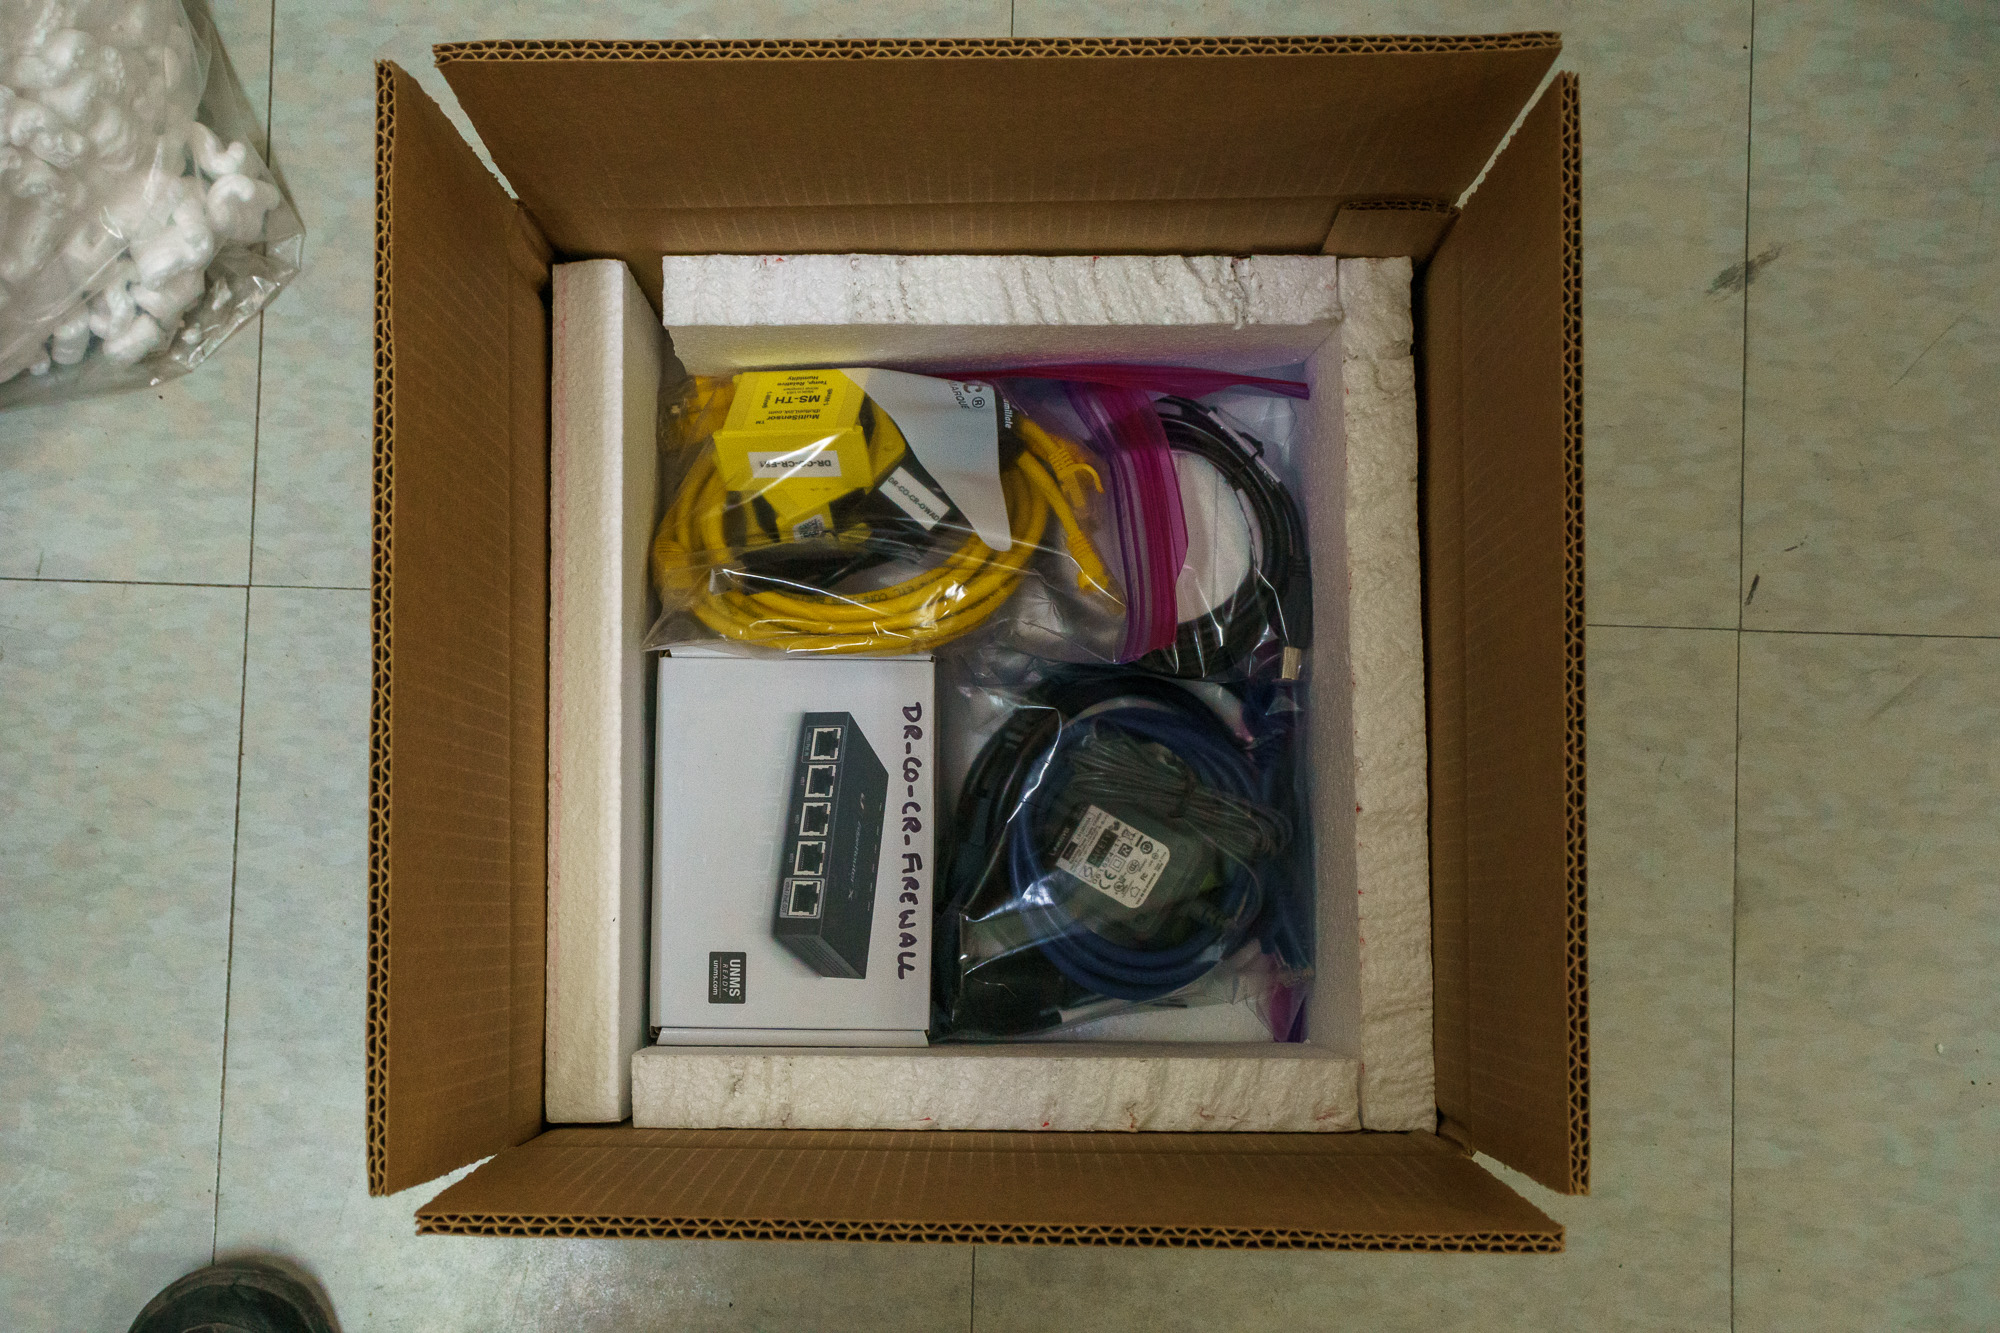
\includegraphics[width=0.60\linewidth]{figures/20201207T172137.jpg}\\[\smallskipamount]
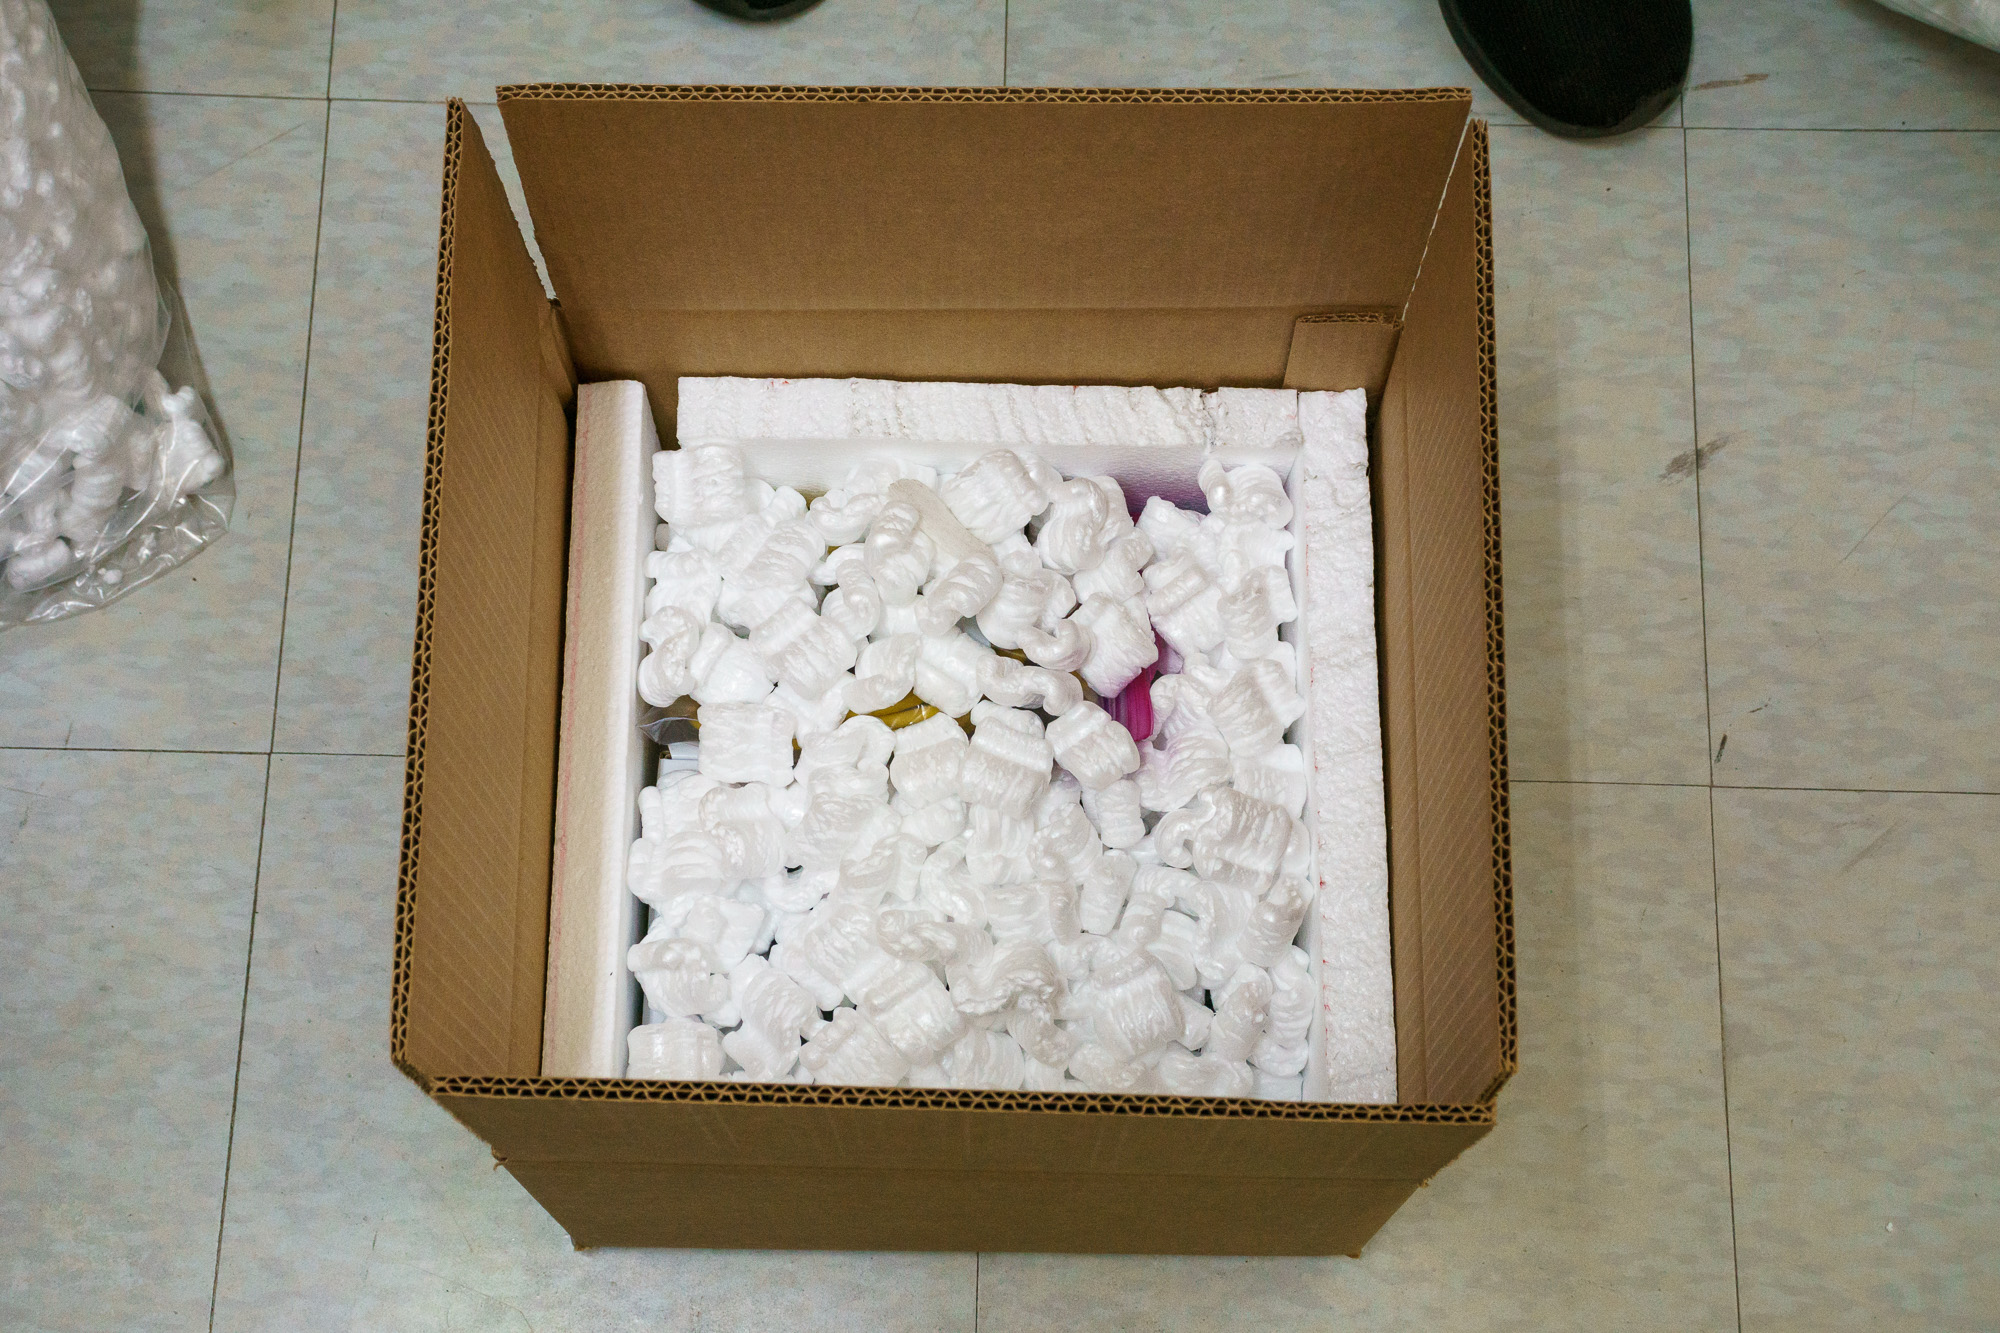
\includegraphics[width=0.60\linewidth]{figures/20201207T172242.jpg}\\[\smallskipamount]
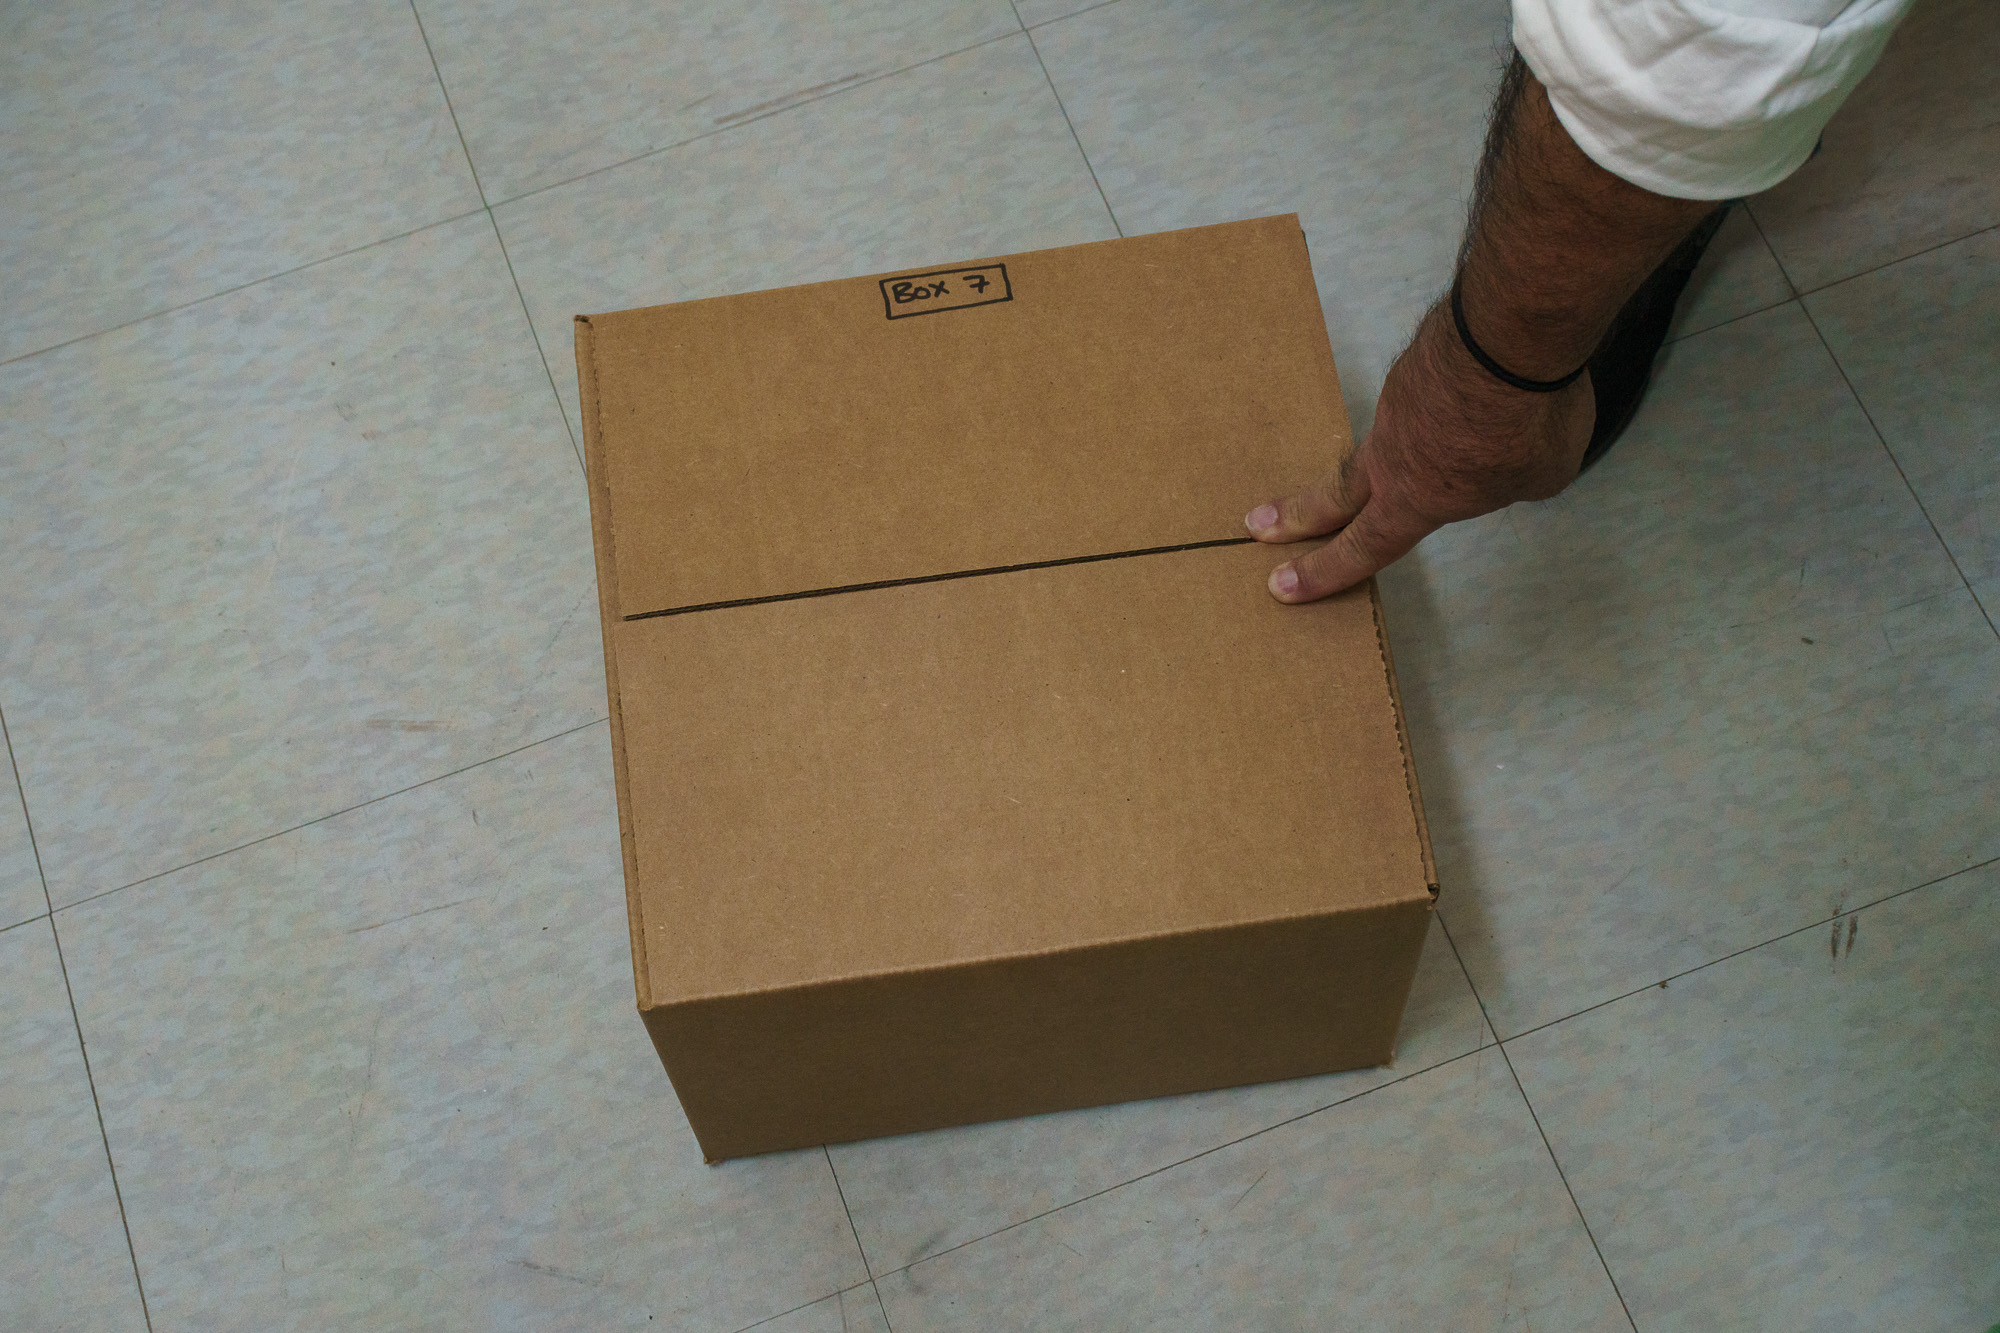
\includegraphics[width=0.60\linewidth]{figures/20201207T172749.jpg}\\[\smallskipamount]
\end{center}
\caption{Box 7 and its contents.}
\label{figure:box-seven-b}
\end{figure}

\subsection{Description}

Box 7 contains:
\begin{itemize}
\item The firewall DR-CO-CR-FIREWALL along with its power supply
DR-CO-CR-FIREWALL-PS, power cable DR-CO-CR-FIREWALL-PWC, extension power cable
DR-CO-CR-FIREWALL-EPWC, and Ethernet cable
DR-CO-CR-FIREWALL-ETHC.
\item The 1-wire adapter DR-CO-CR-OWAD.
\item The two 1-wire sensors for the control room rack 
DR-CO-CR-ES1 and
DR-CO-CR-ES2
along with the three yellow 1-wire cables 
DR-CO-CR-ES1-OWC,
DR-CO-CR-ES2-OWC, and
DR-CO-CR-ES3-OWC.
\item The USB extender LEX 
DR-CO-CR-USBLEX and its USB cable
DR-CO-CR-USBLEX-USBC.
\end{itemize}

The firewall is packed first in its original box. The contents are then packed in a cardboard box lined on all sides with 25~mm polystyrene foam sheets and filled with polystyrene packing peanuts. See Figure~\ref{figure:box-seven-a} and \ref{figure:box-seven-b}.

Box 7 is $30 \times 30 \times 30 \times 20$~cm ($L \times W \times H$) and has a weight of 2 kg.

\subsection{Unpacking Instructions}

There are no special unpacking instructions.

\subsection{Repacking Instructions}

There are no special repacking instructions.

%%%%%%%%%%%%%%%%%%%%%%%%%%%%%%%%%%%%%%%%%

\clearpage
\section{Box 8}

\begin{figure}[bp]
\begin{center}
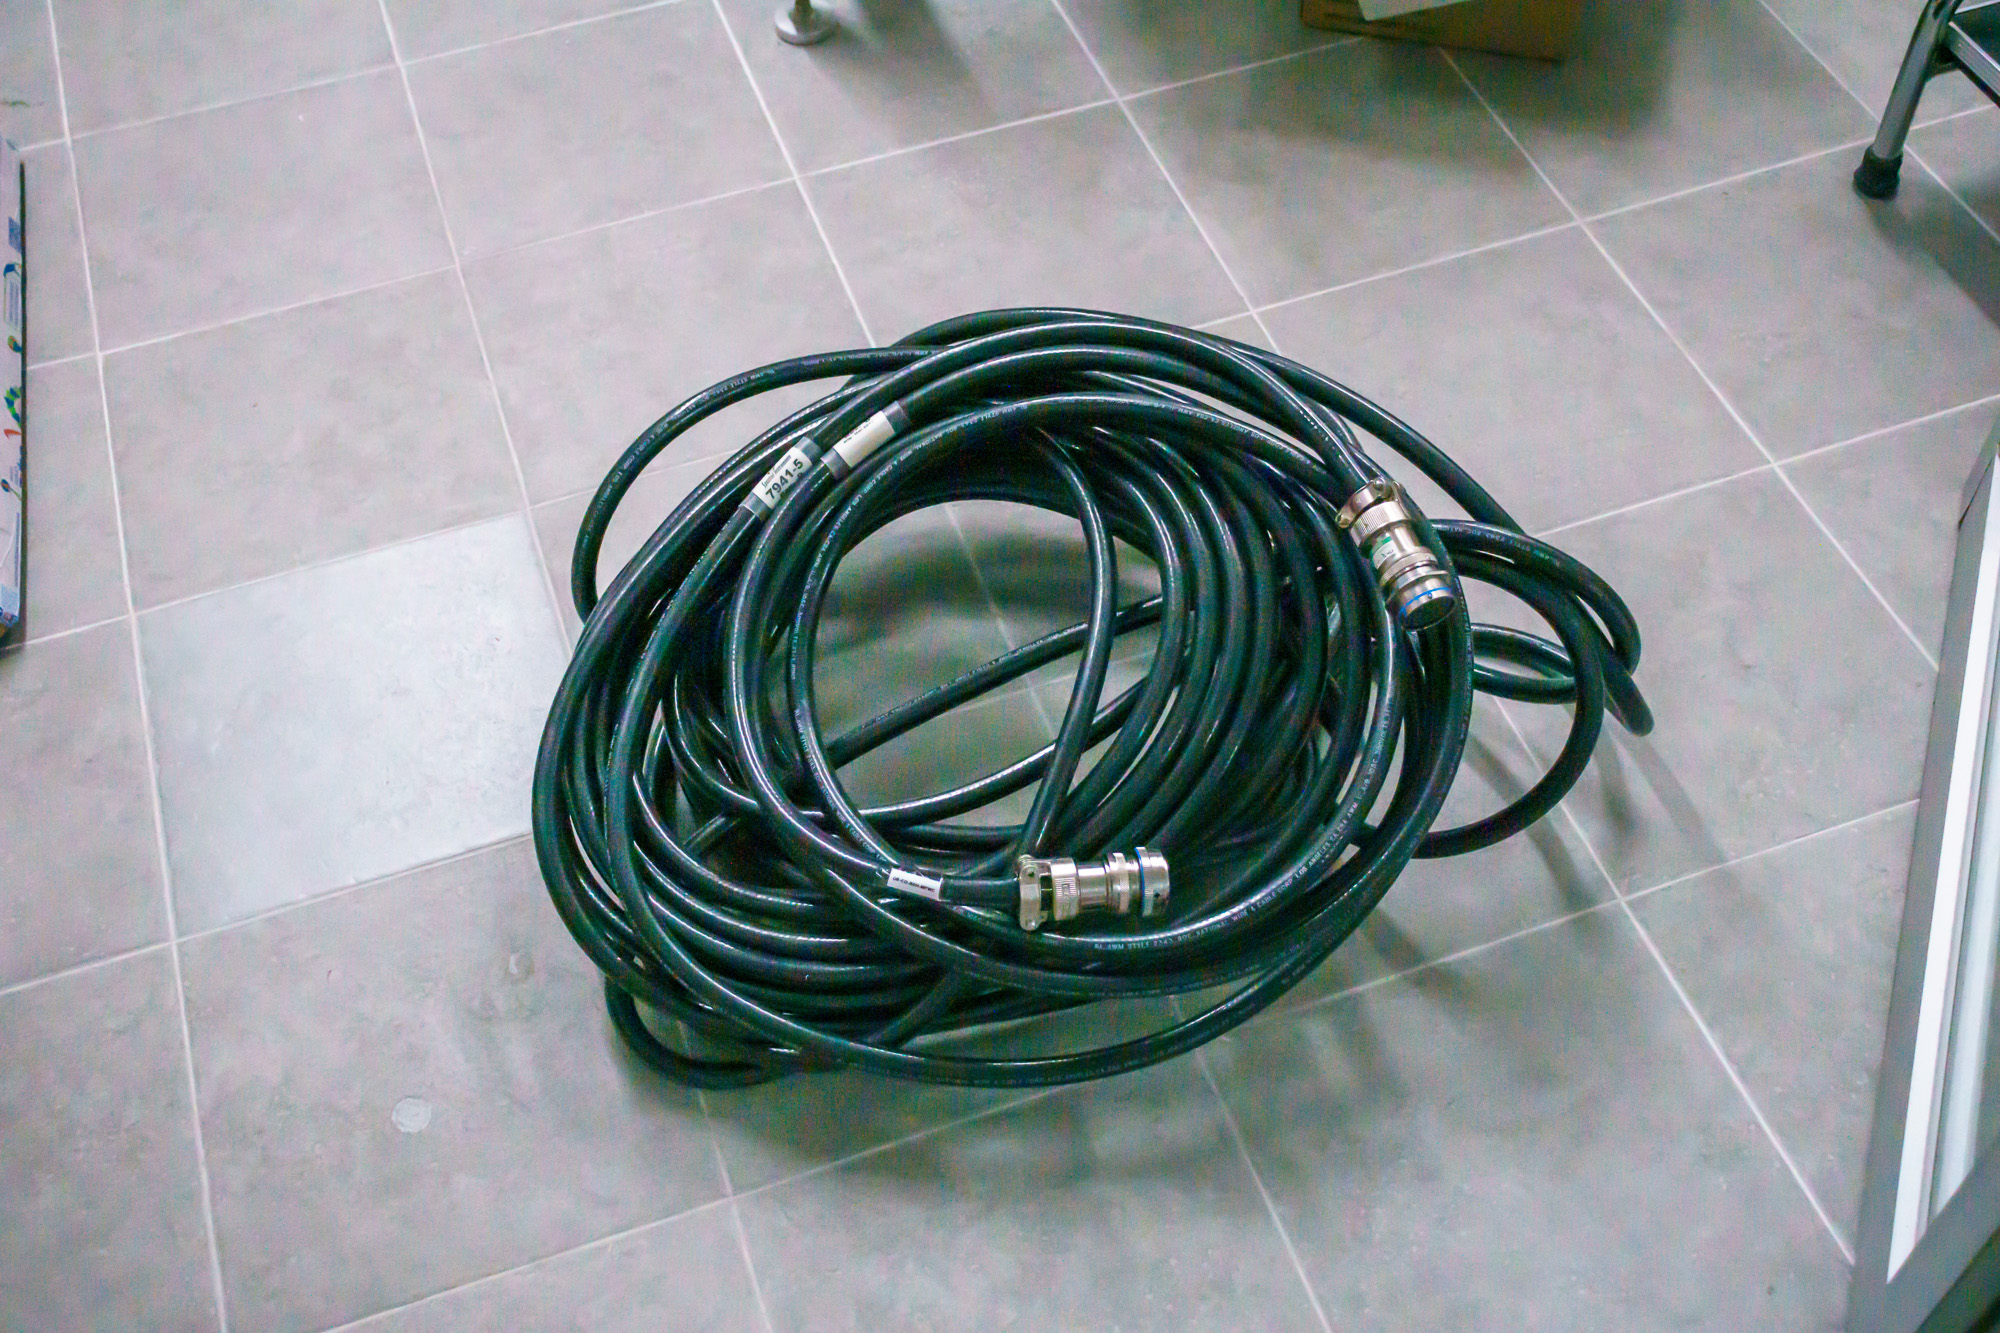
\includegraphics[width=0.45\linewidth]{figures/20201207T191558.jpg}
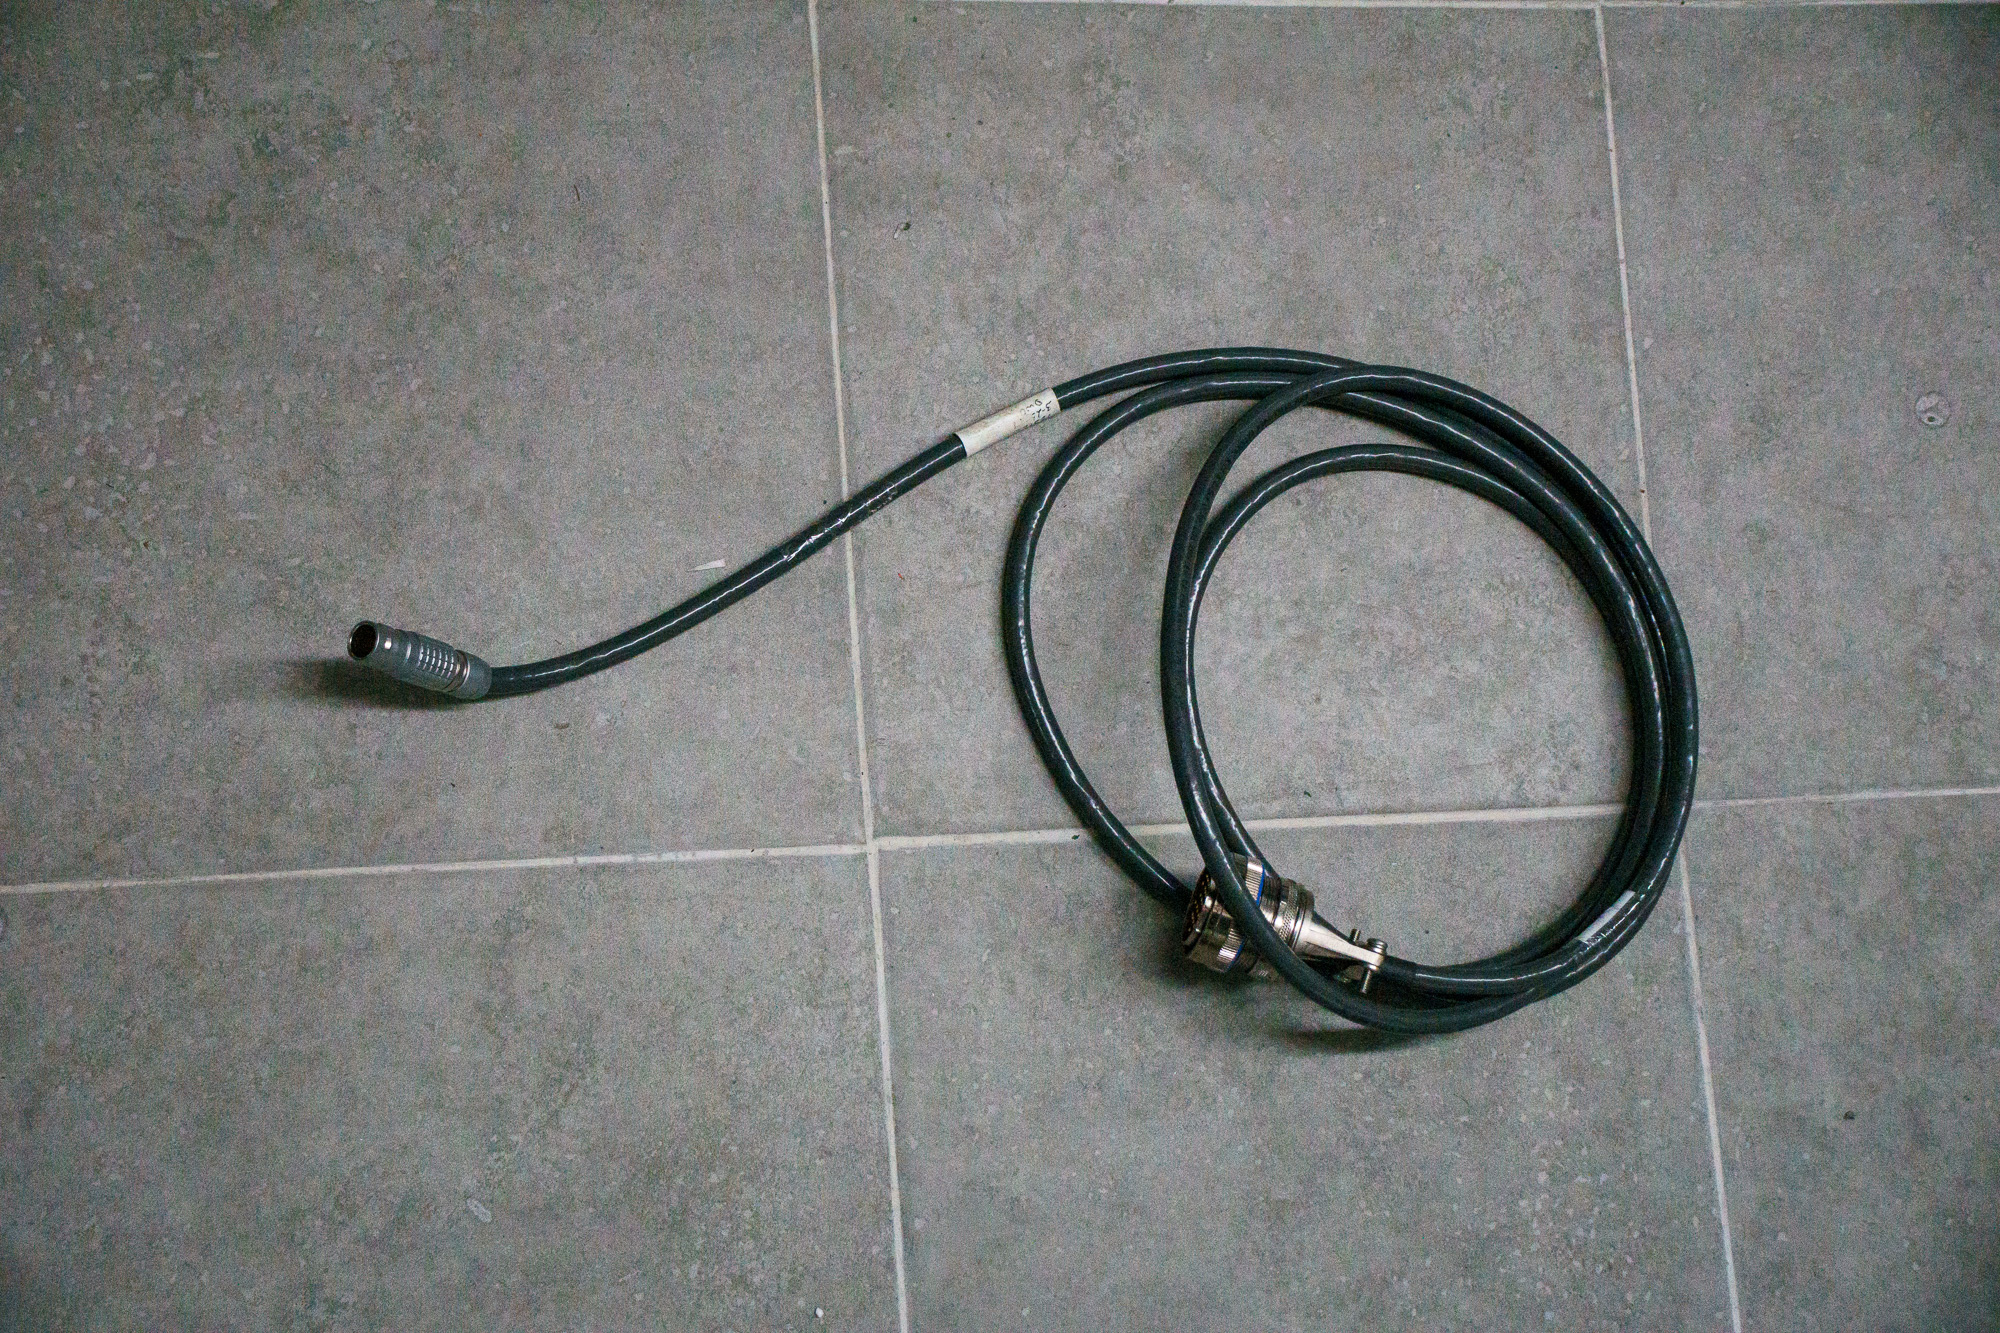
\includegraphics[width=0.45\linewidth]{figures/20201207T191616.jpg}
\end{center}
\caption{Box 8 contents. Left: The blue detector main power cable DR-CO-BDH-MPWC. Right: The blue detector extension power cable DR-CO-BDH-EPWC.}
\label{figure:box-eight-contents}
\end{figure}

\begin{figure}[bp]
\begin{center}
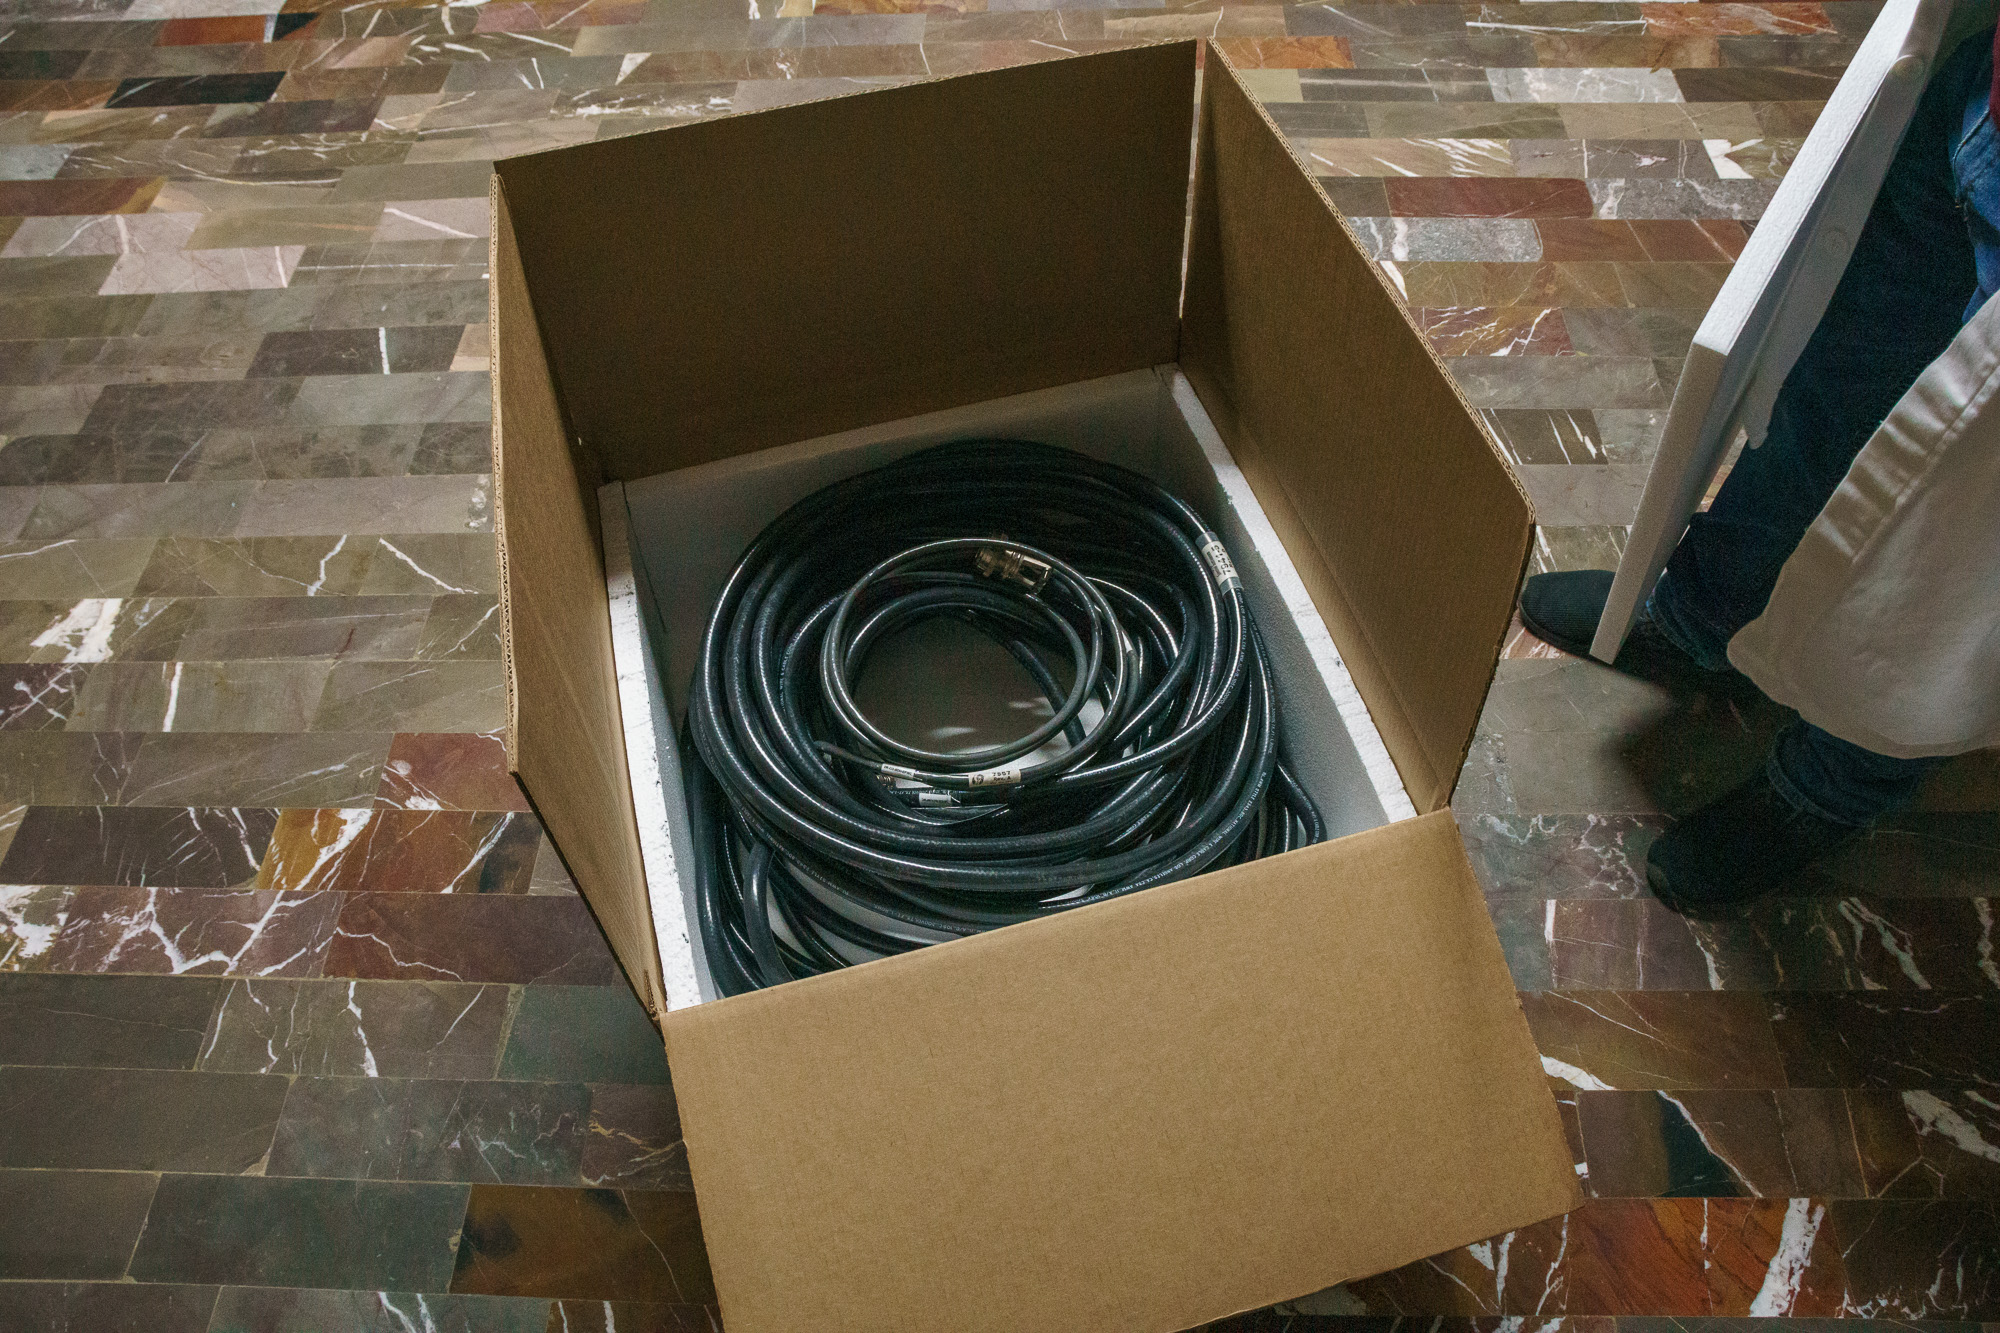
\includegraphics[width=0.30\linewidth]{figures/20201207T192420.jpg}
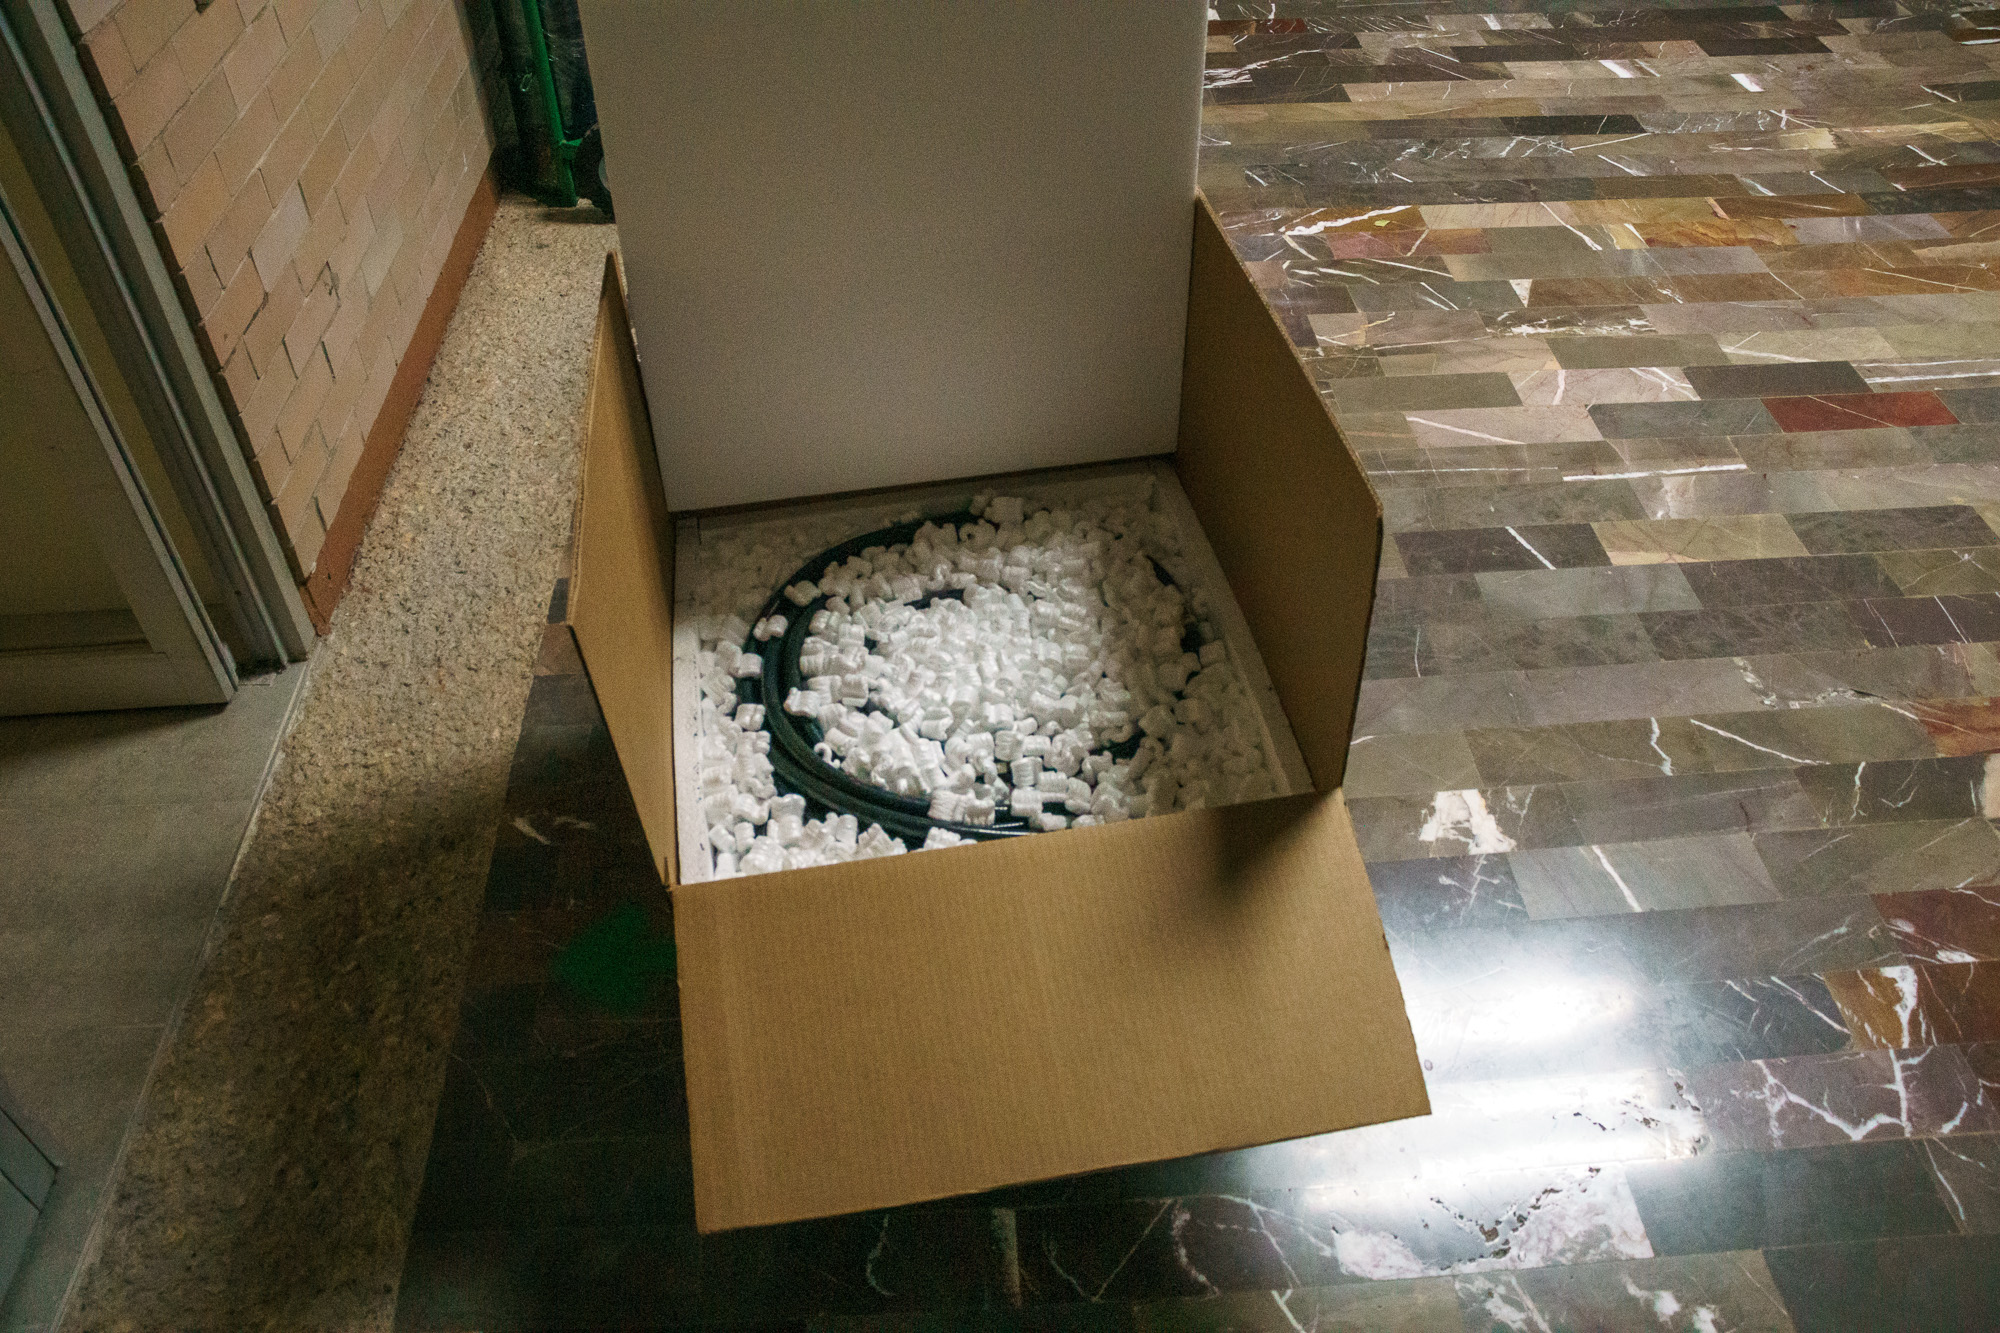
\includegraphics[width=0.30\linewidth]{figures/20201207T192712.jpg}
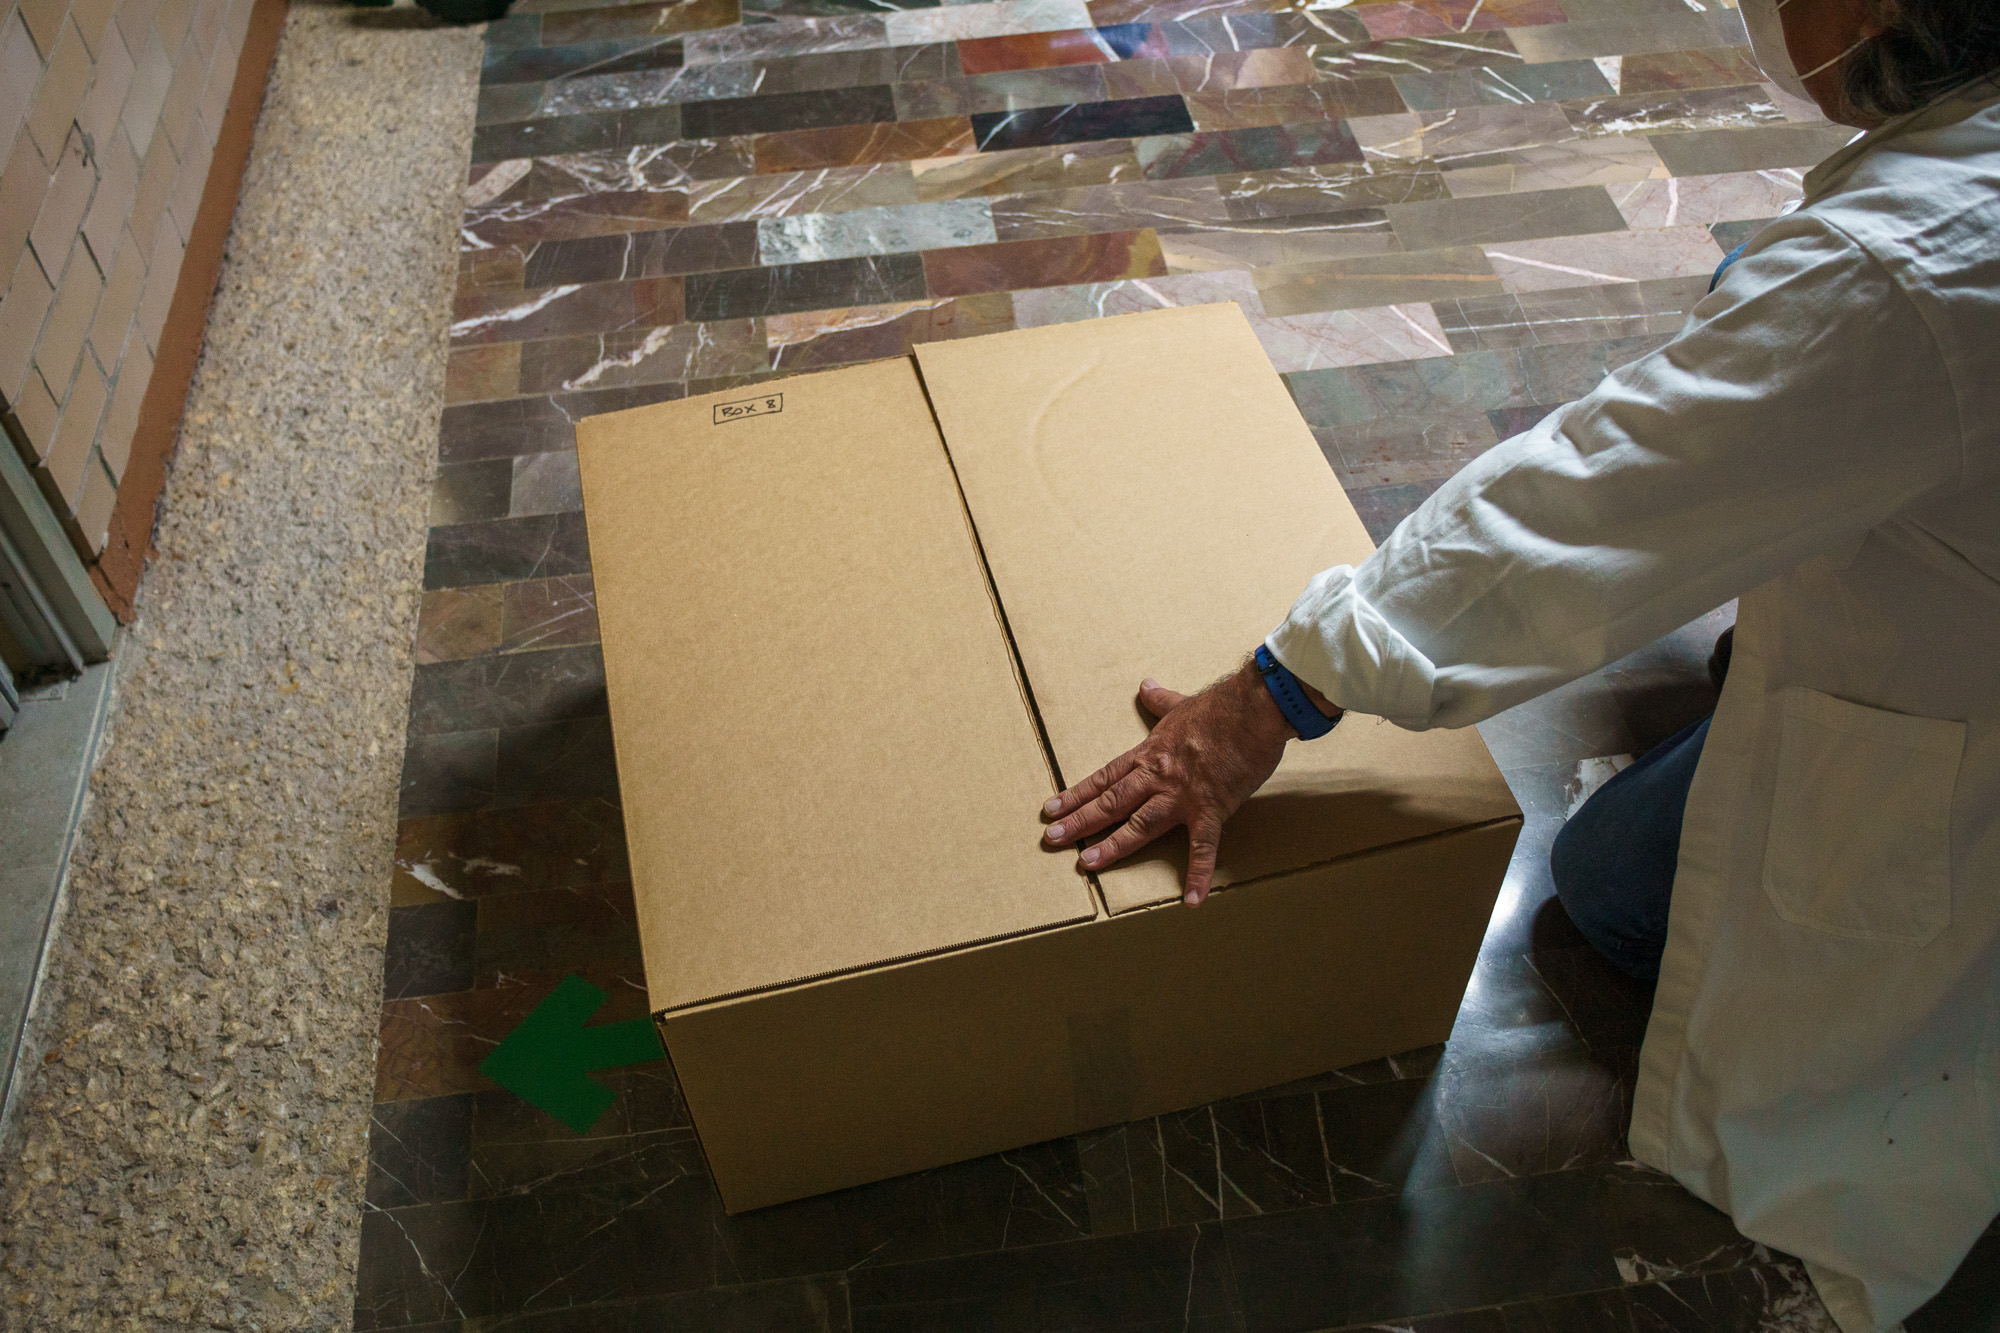
\includegraphics[width=0.30\linewidth]{figures/20201207T192933.jpg}
\end{center}
\caption{Box 8 packing.}
\label{figure:box-eight-packing}
\end{figure}

\subsection{Description}

Box 8 contains:

\begin{itemize}
    \item The blue detector power cables DR-CO-BDH-MPWC and DR-CO-BDH-EPWC.
\end{itemize}

The cables are packed into a cardboard box lined on all sides with 25~mm polystyrene foam sheets and filled with polystyrene packing peanuts. See Figure~\ref{figure:box-eight-contents}.

Box 8 is  $60 \times 60 \times 30$~cm ($L \times W \times H$) and has a weight of 27 kg.

\subsection{Unpacking Instructions}

There are no special unpacking instructions.

\subsection{Repacking Instructions}

There are no special repacking instructions.

%%%%%%%%%%%%%%%%%%%%%%%%%%%%%%%%%%%%%%%%%

\clearpage
\section{Box 9}

\begin{figure}[bp]
\begin{center}
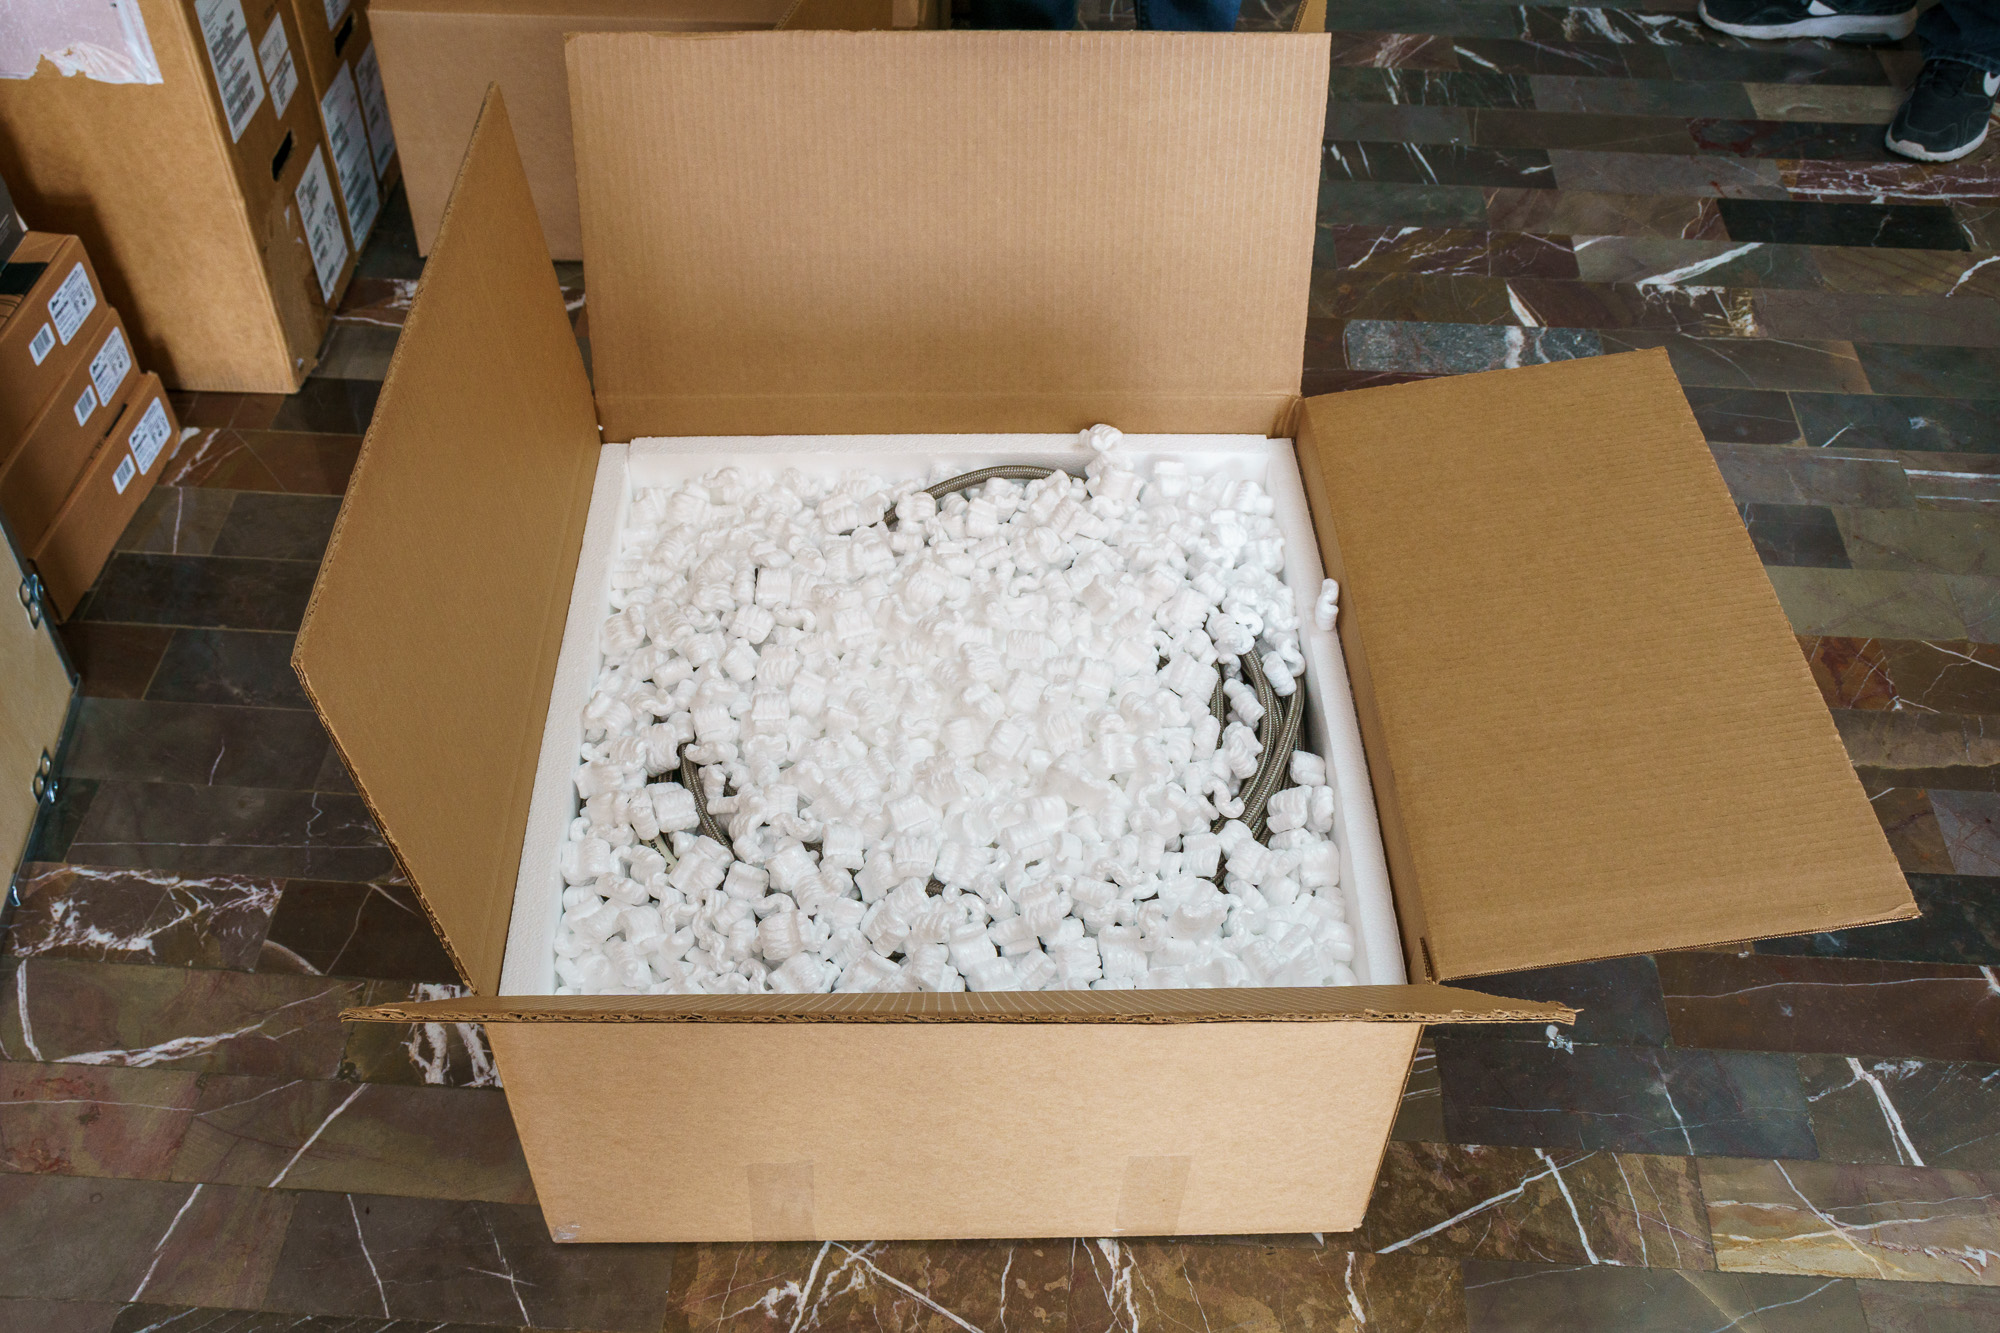
\includegraphics[width=0.60\linewidth]{figures/20201209T115319.jpg}\\[\smallskipamount]
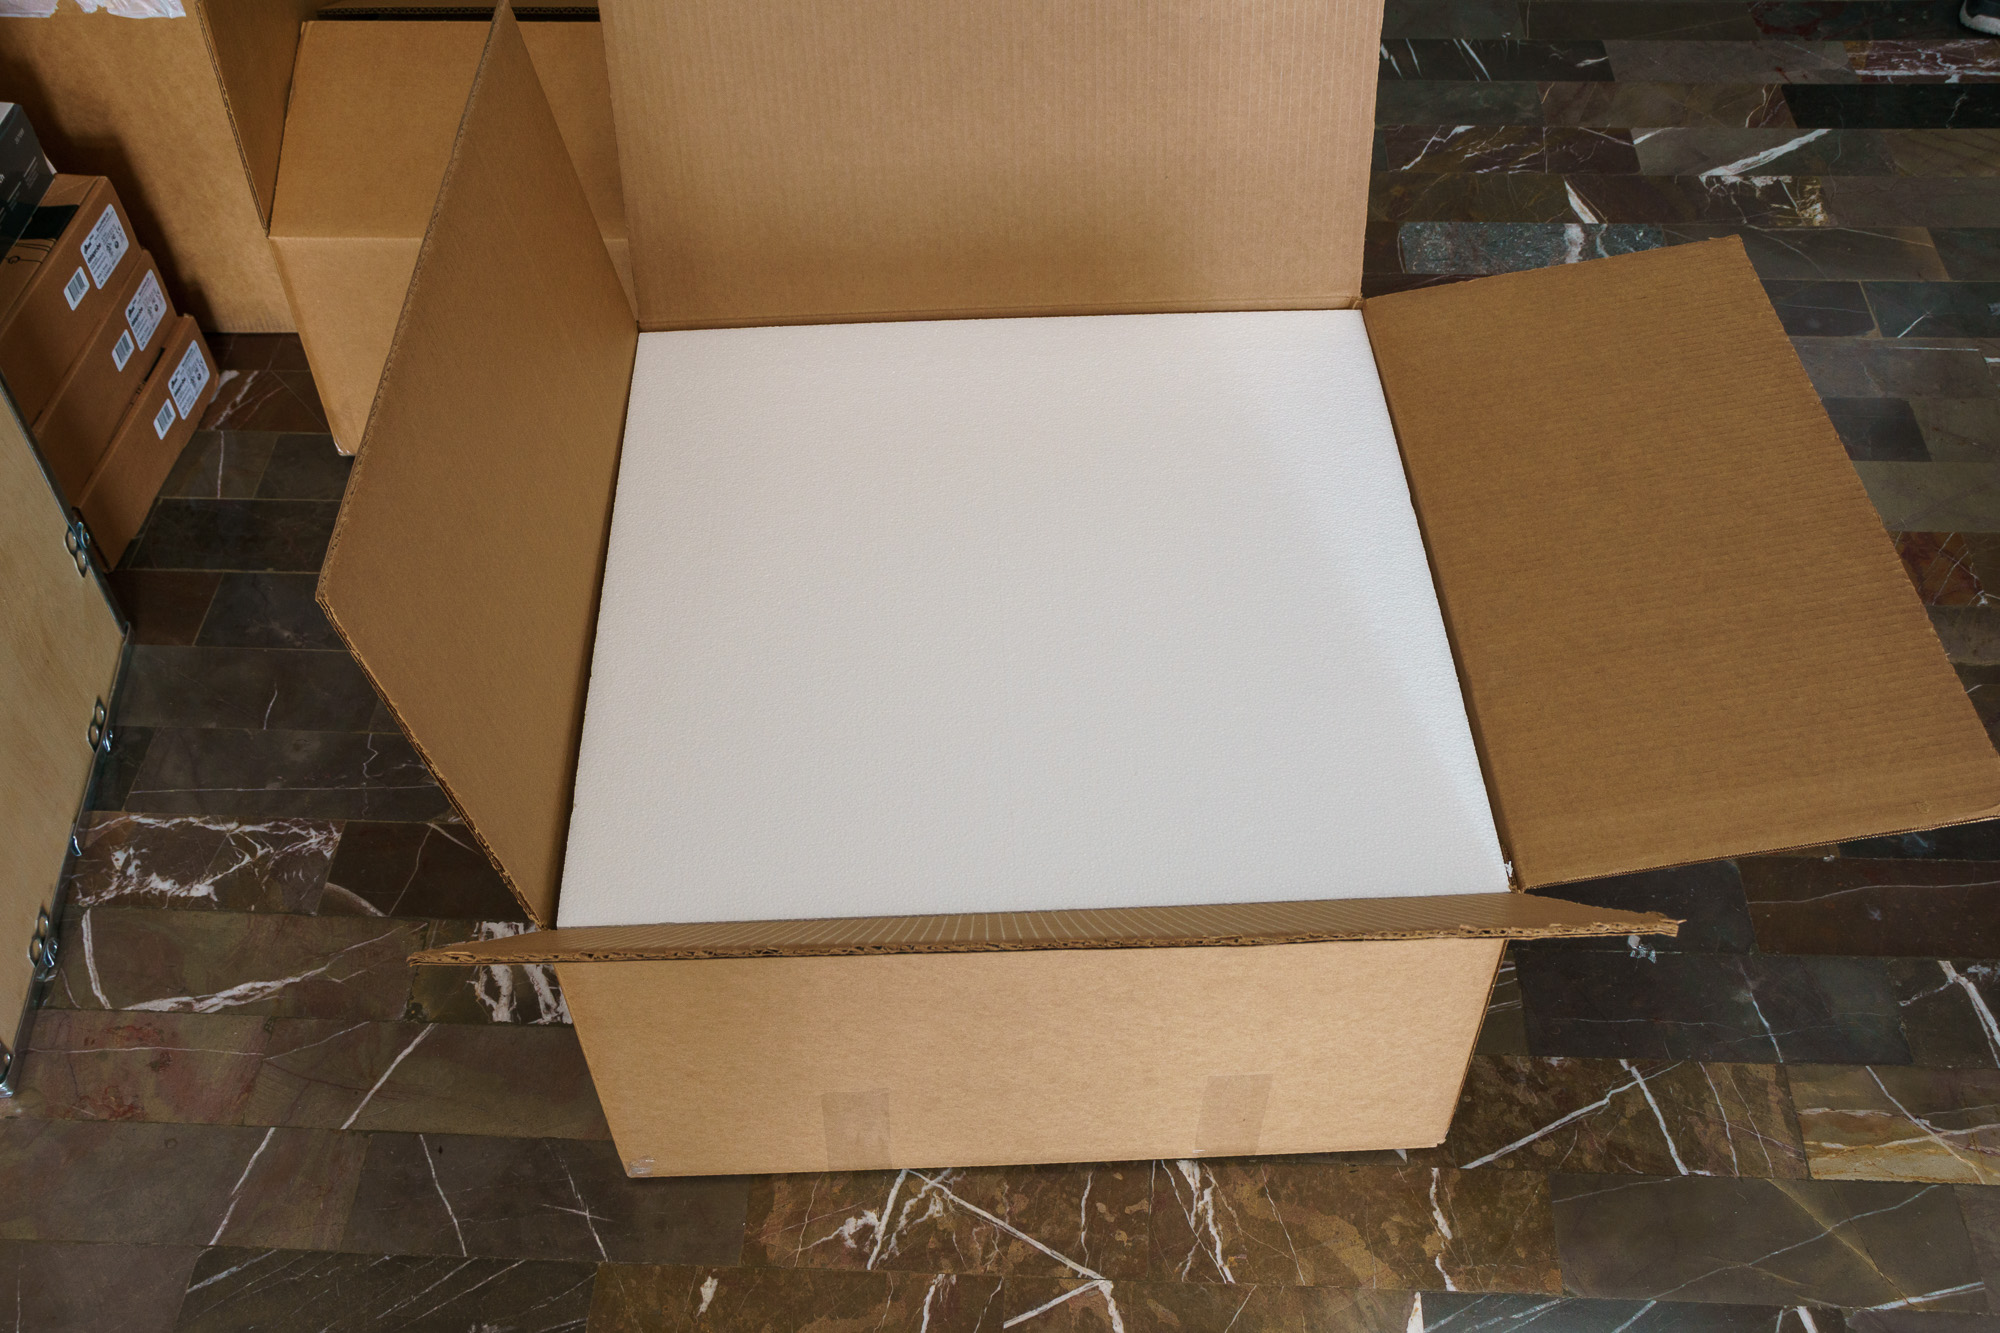
\includegraphics[width=0.60\linewidth]{figures/20201209T115331.jpg}\\[\smallskipamount]
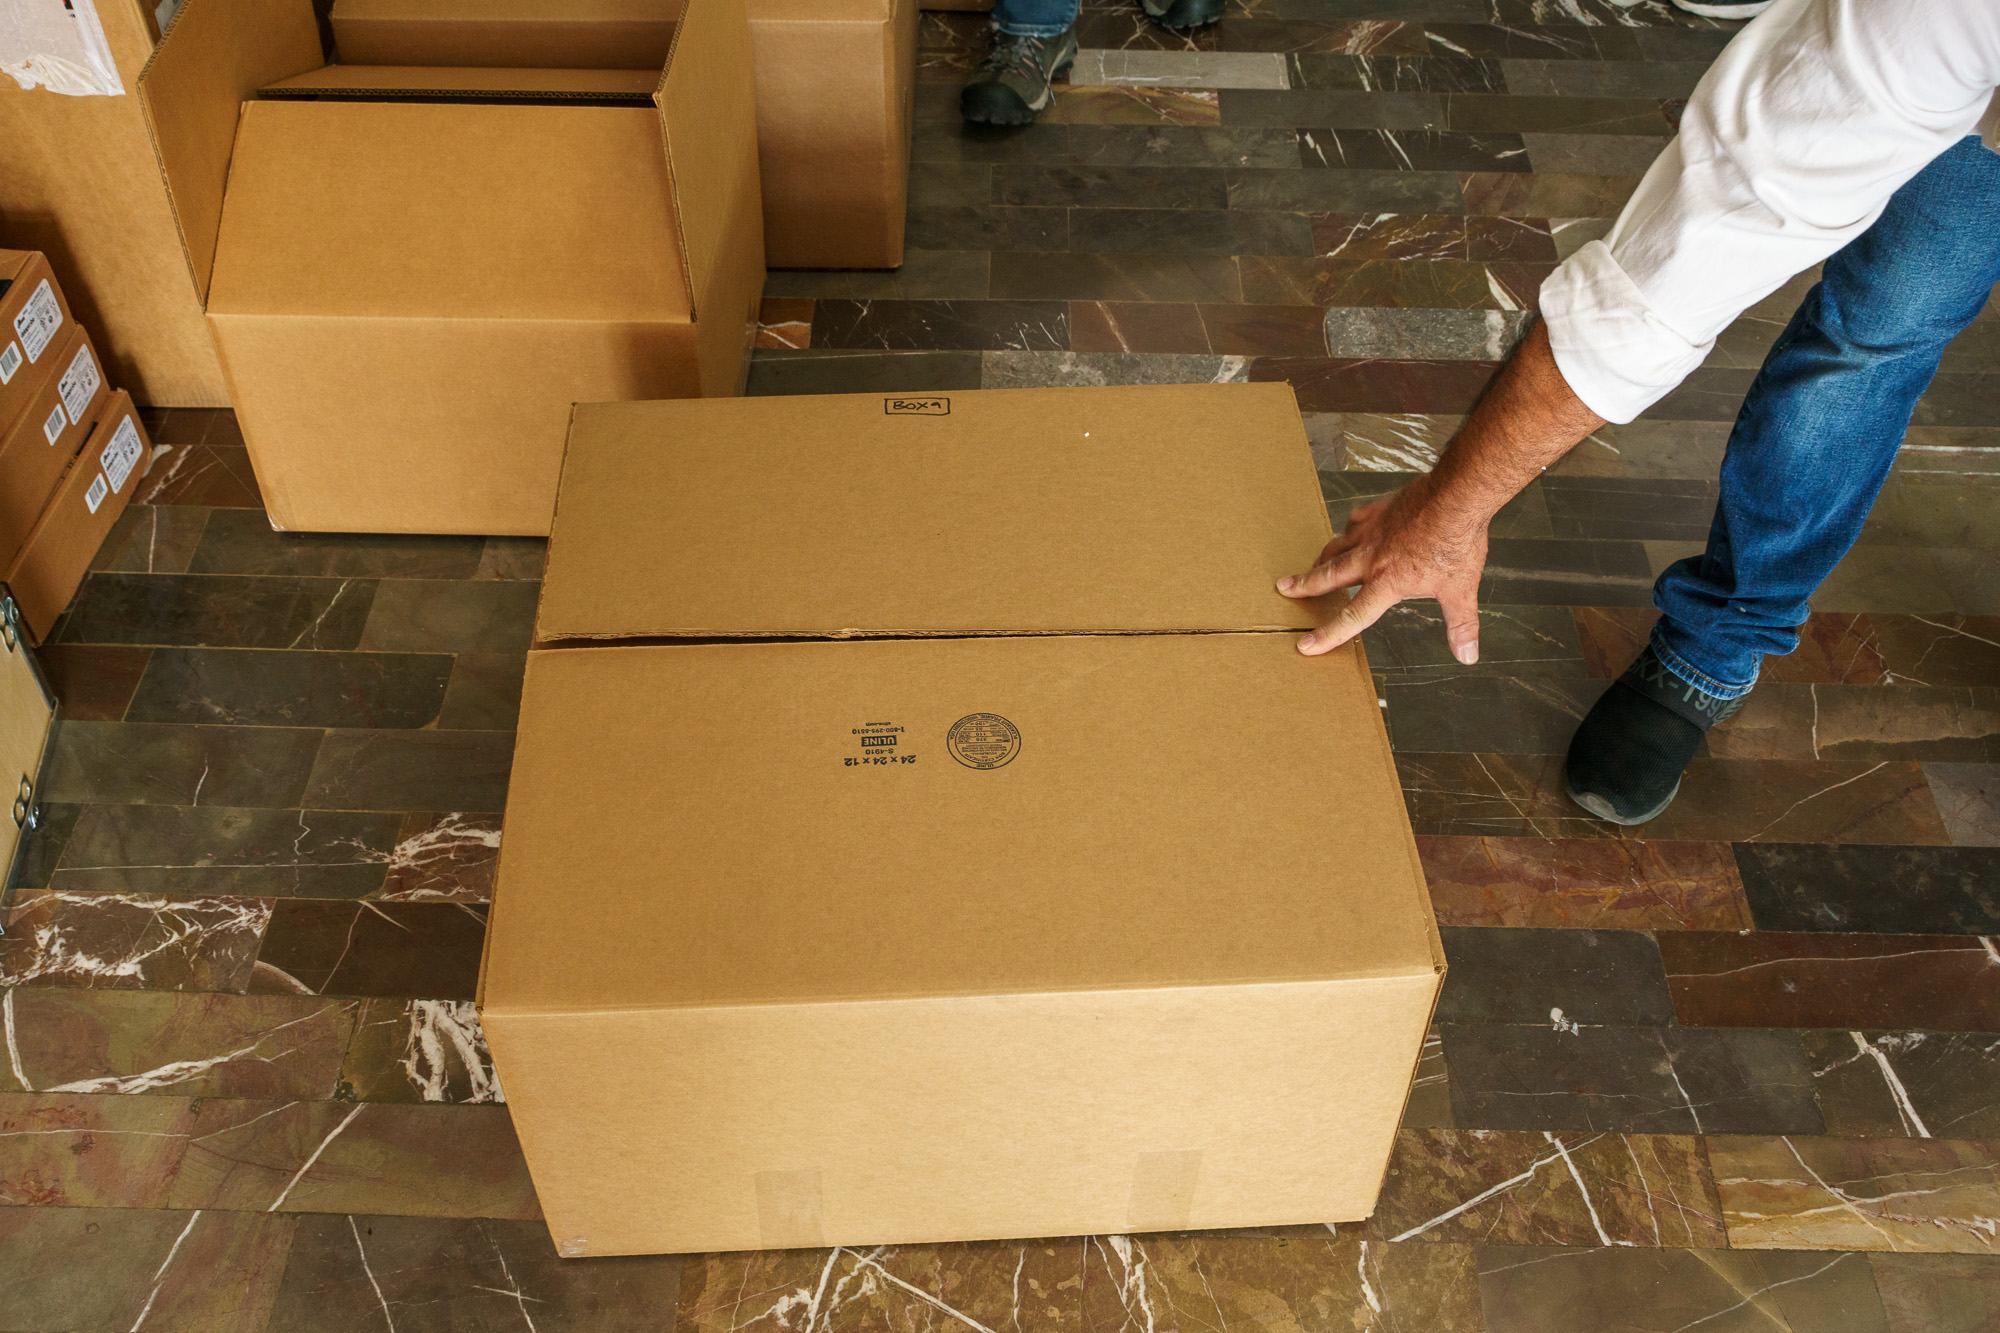
\includegraphics[width=0.60\linewidth]{figures/20201209T115337.jpg}
\end{center}
\caption{Box 9 and its contents.}
\label{figure:box-nine}
\end{figure}

\subsection{Description}

Box 9 contains:

\begin{itemize}
    \item The blue detector cryogen supply and return hoses DR-CO-BDH-CHS and DR-CO-BDH-CHR.
\end{itemize}

The hoses are packed into a cardboard box lined on all sides with 25~mm polystyrene foam sheets and filled with polystyrene packing peanuts. See Figure~\ref{figure:box-nine}.

Box 9 is  $60 \times 60 \times 30$~cm ($L \times W \times H$) and has a weight of 15 kg.

\subsection{Unpacking Instructions}

There are no special unpacking instructions, except to remember not to twist the cables when uncoiling them.

\subsection{Repacking Instructions}

There are no special repacking instructions, except to remember not to twist the cables when coiling them.

%%%%%%%%%%%%%%%%%%%%%%%%%%%%%%%%%%%%%%%%%

\clearpage
\section{Box 10}

\begin{figure}[bp]
\begin{center}
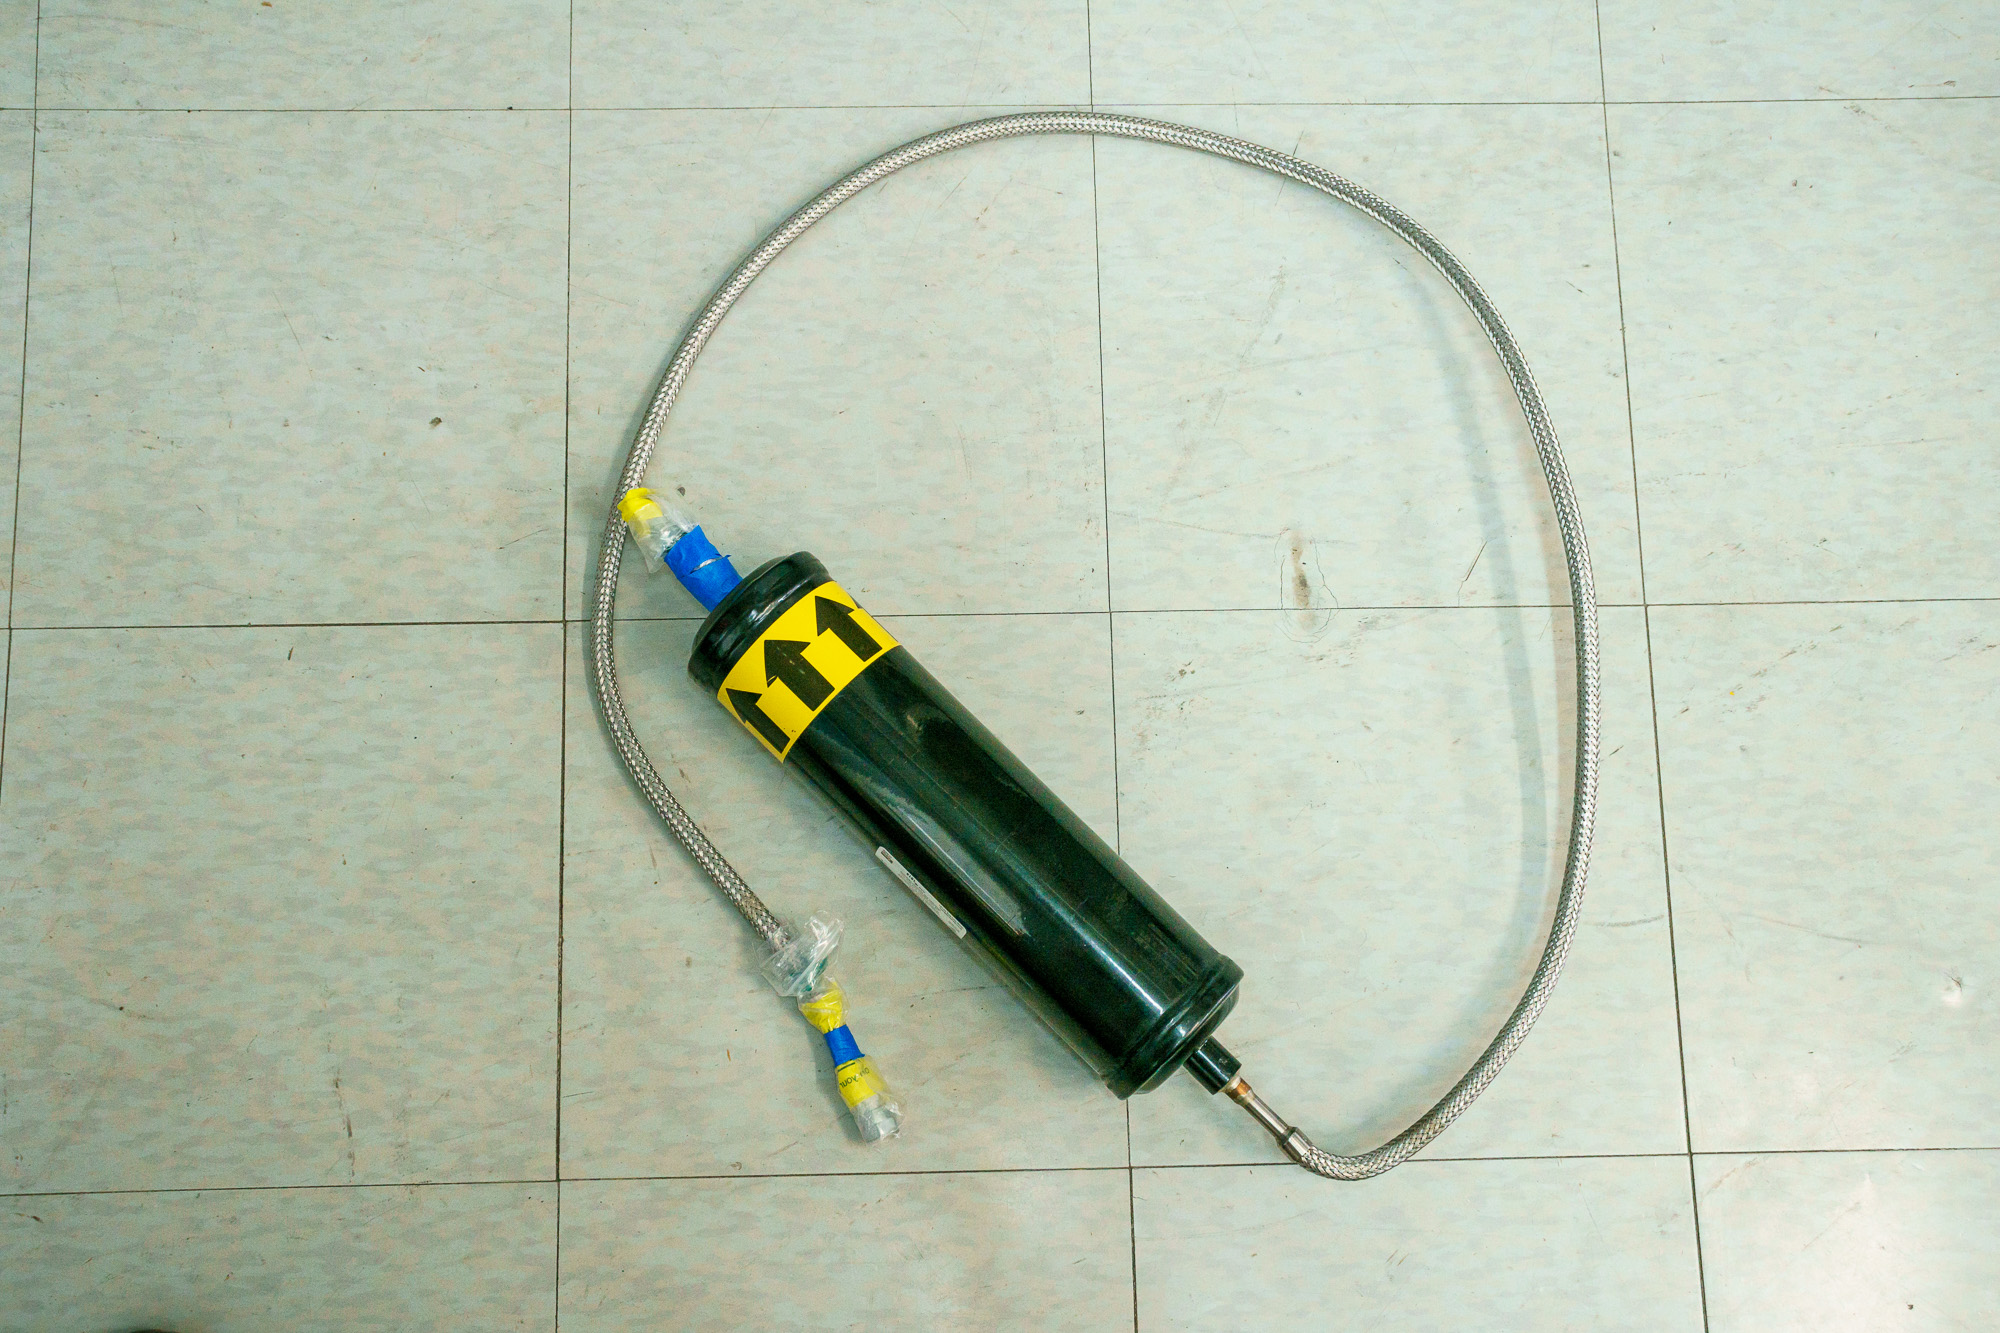
\includegraphics[width=0.45\linewidth]{figures/20201209T123146.jpg}
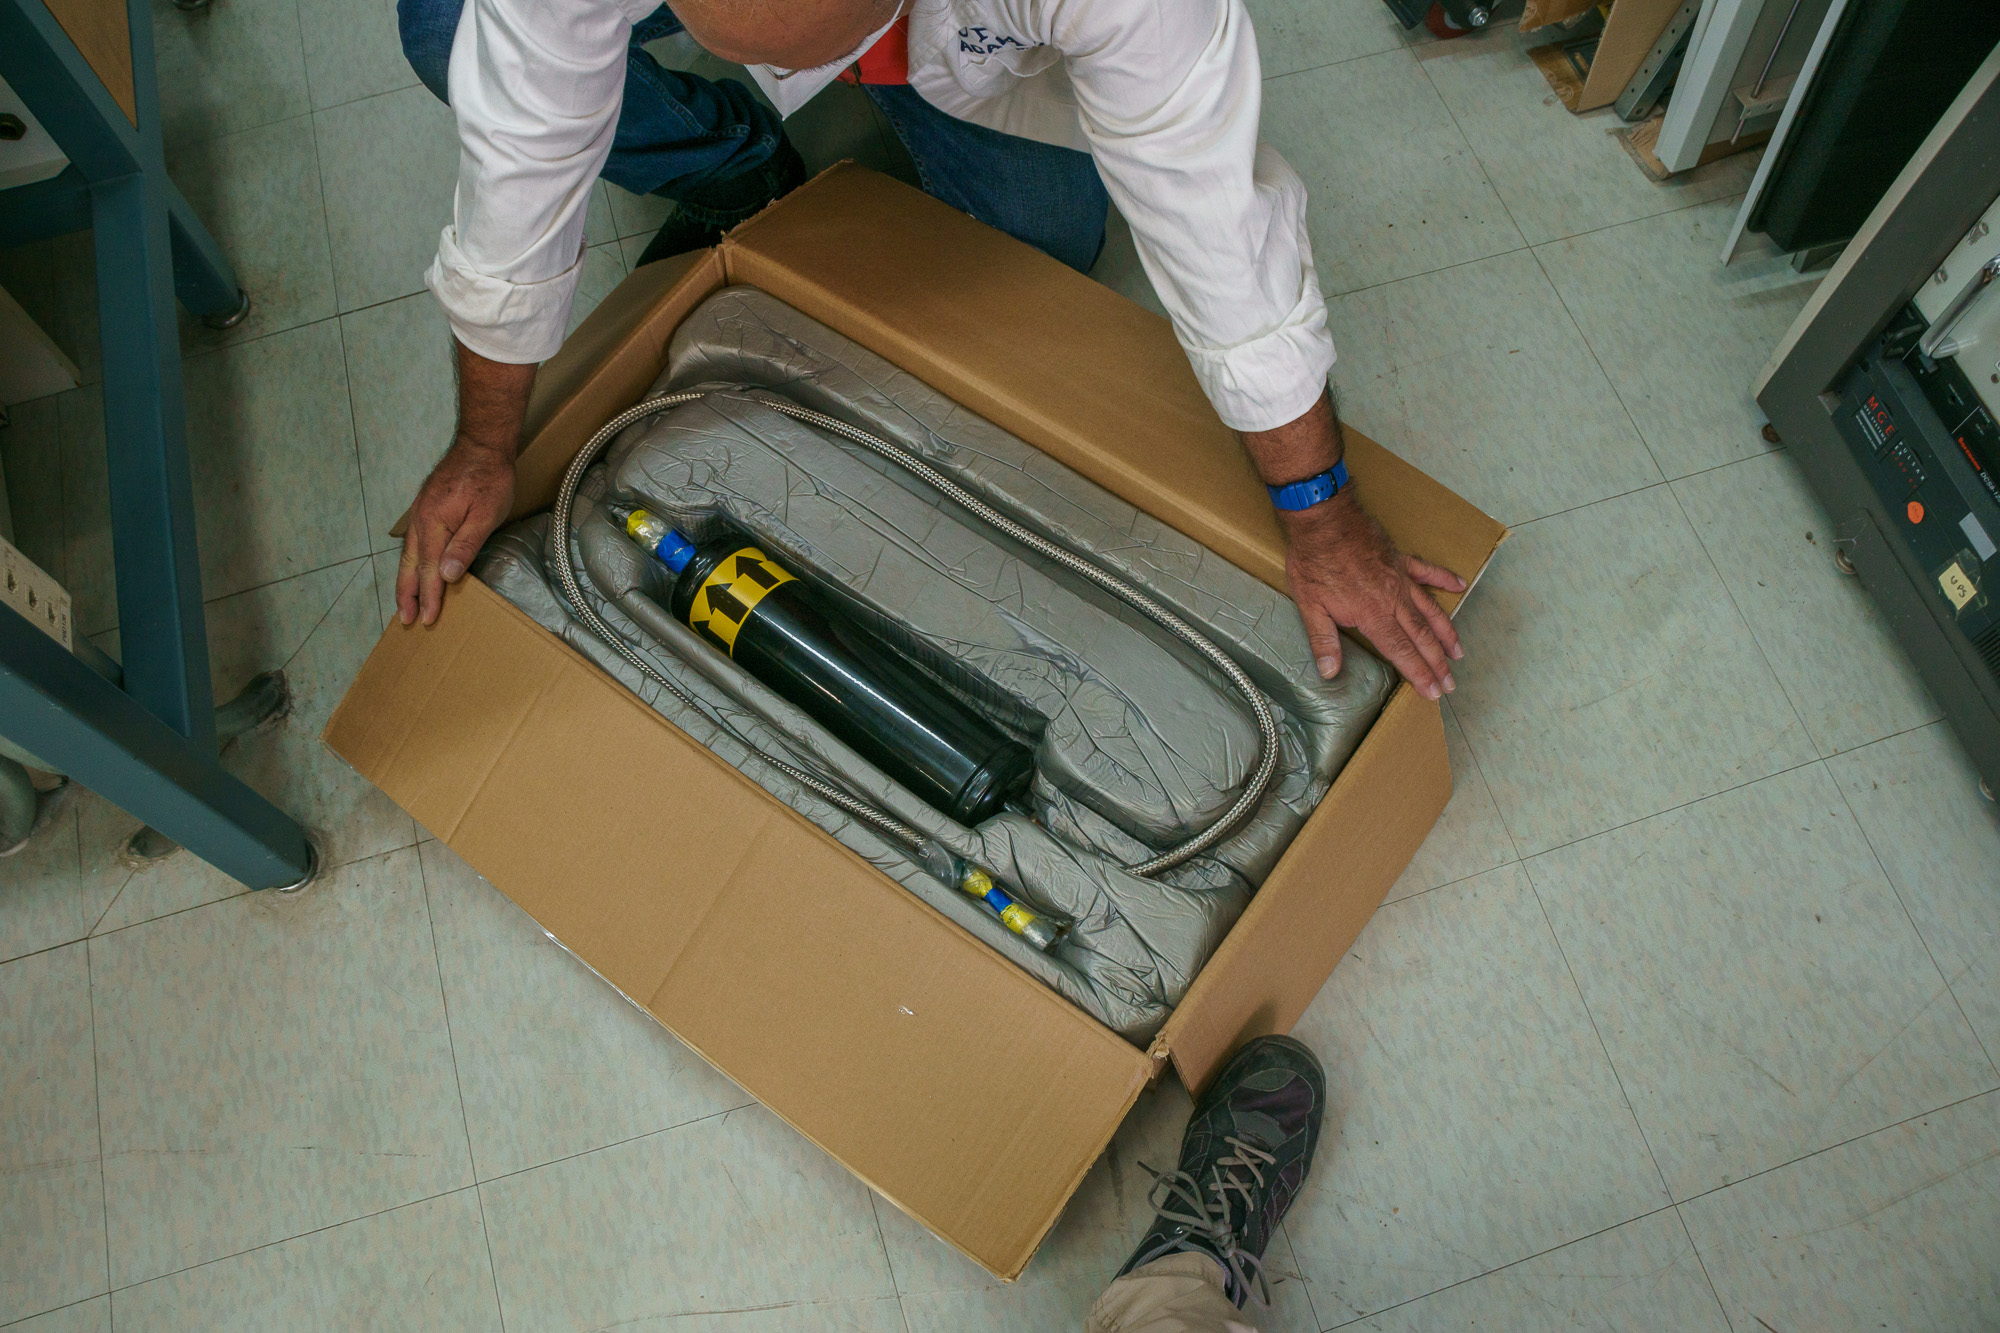
\includegraphics[width=0.45\linewidth]{figures/20201209T123225.jpg}\\[\smallskipamount]
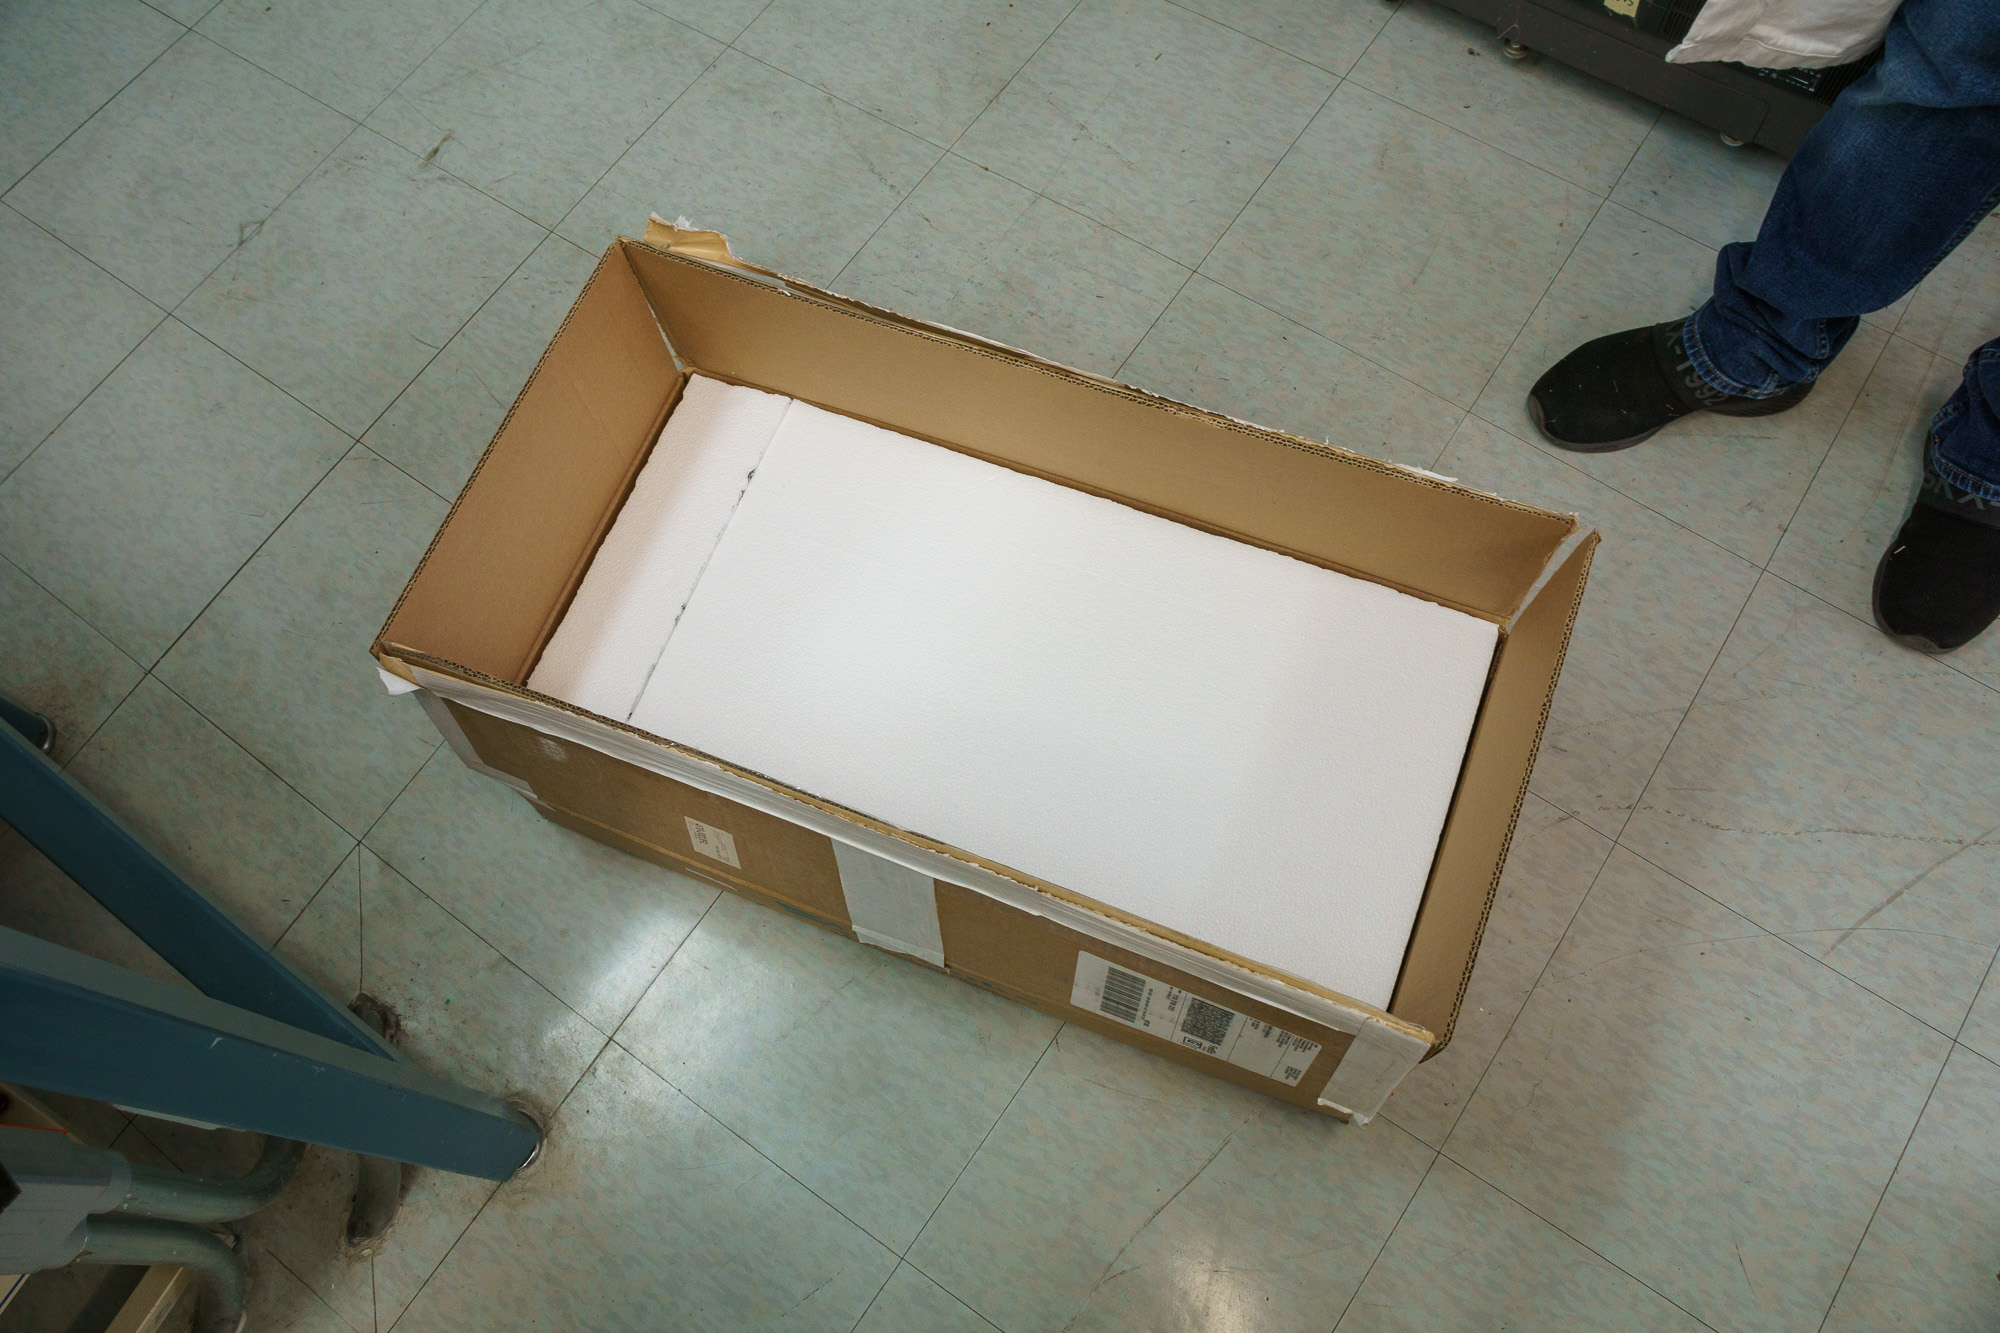
\includegraphics[width=0.45\linewidth]{figures/20201209T123910.jpg}
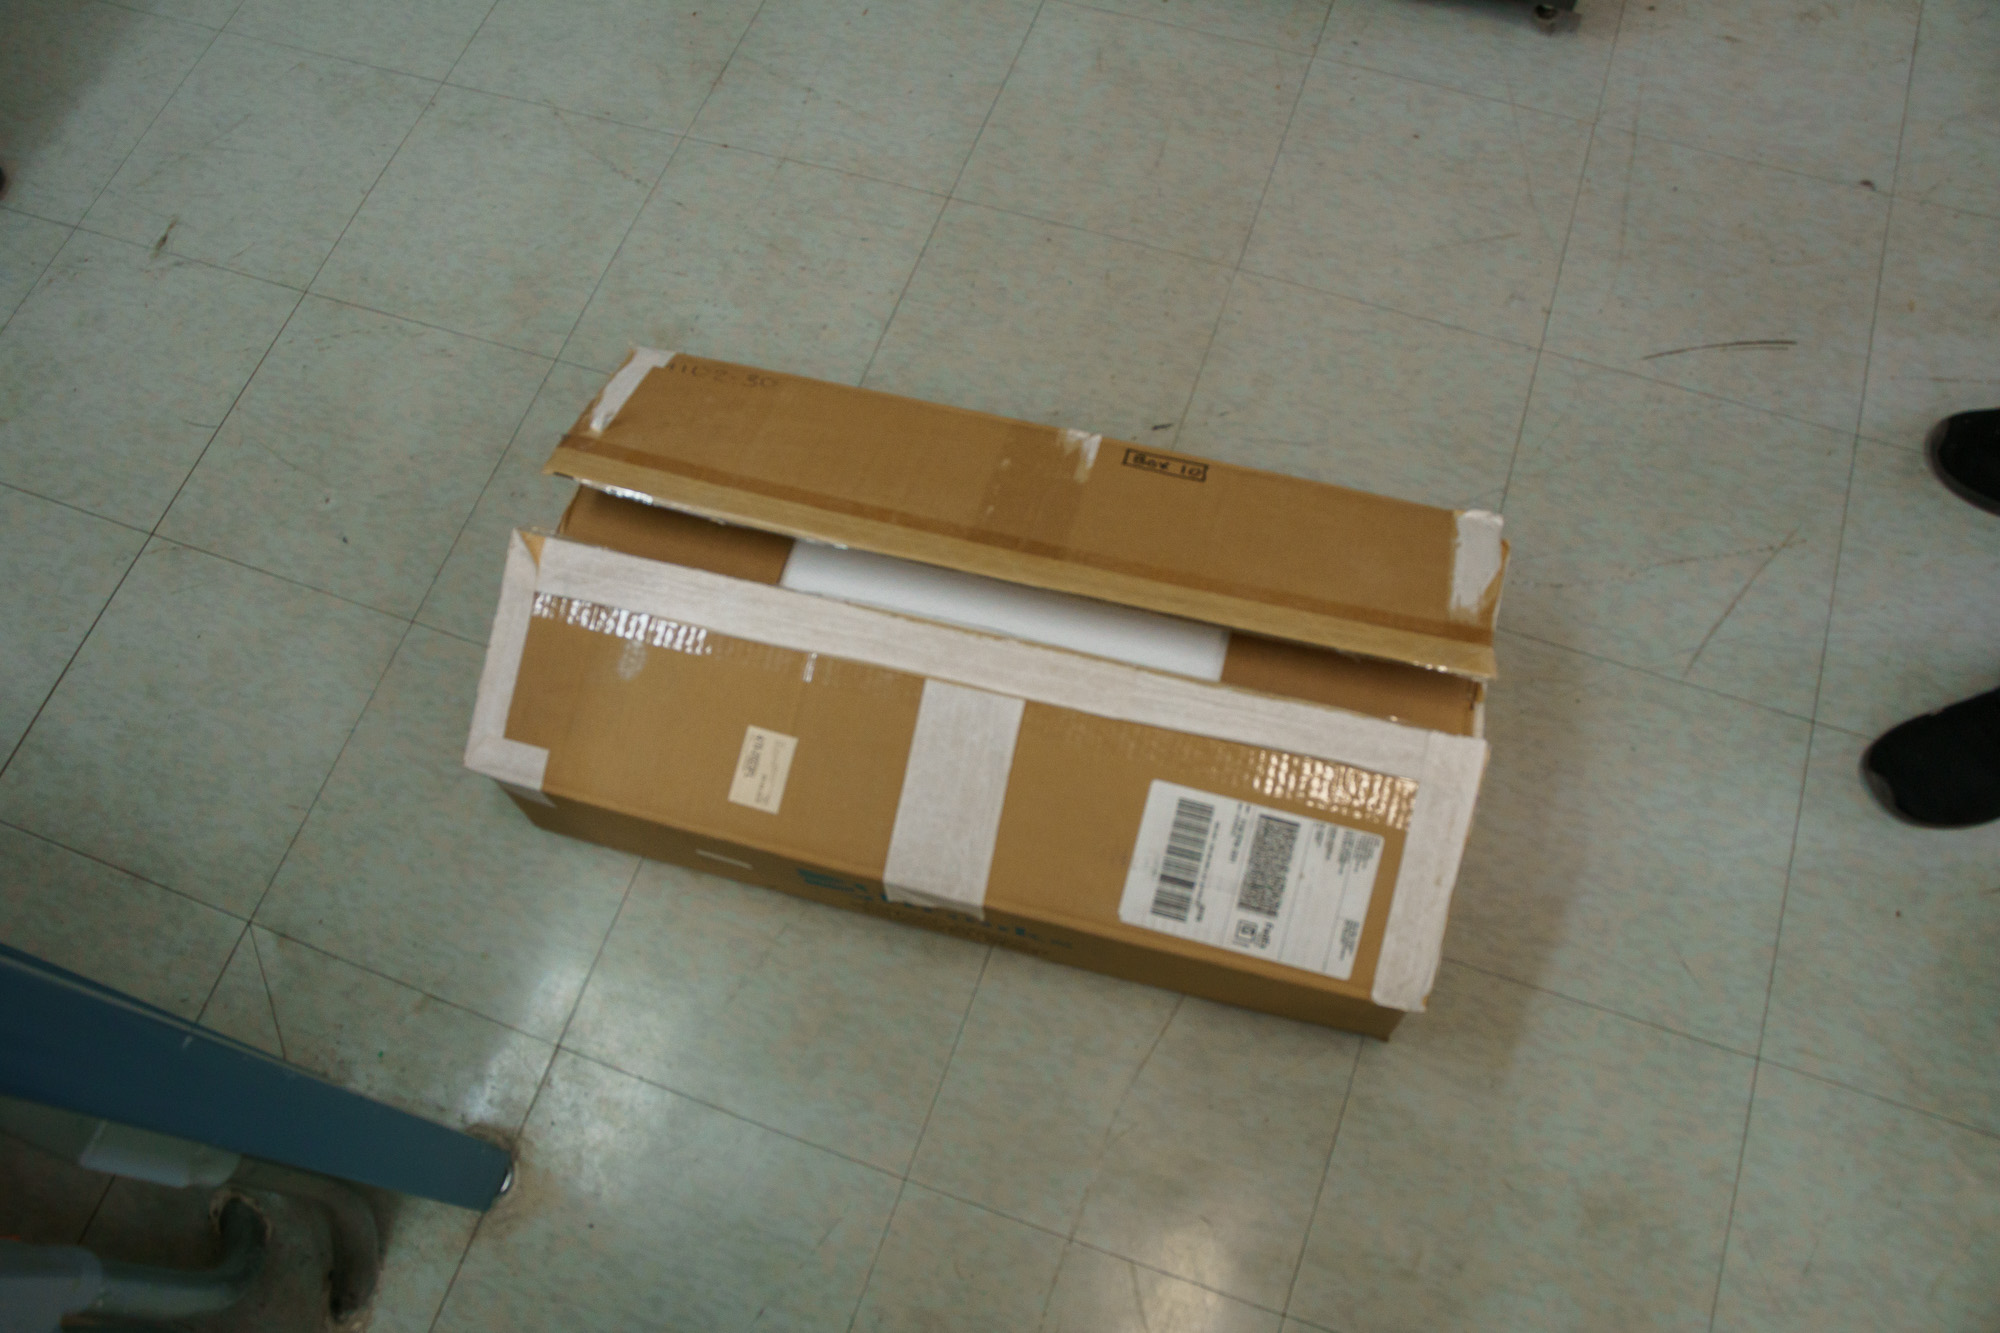
\includegraphics[width=0.45\linewidth]{figures/20201209T123946.jpg}\\[\smallskipamount]
\end{center}
\caption{Box 10 and its contents.}
\label{figure:box-ten}
\end{figure}

\subsection{Description}

Box 10 contains:

\begin{itemize}
    \item The blue service cabinet dryer and filter DR-CO-CR-BDSC-DRFL.
\end{itemize}

The dryer and filter is packed into a cardboard box with a custom foam liner and a 25~mm foam sheet lid. See Figure~\ref{figure:box-ten}.

Box 10 is $75 \times 40 \times 20$~cm ($L \times W \times H$) and has a weight of 5 kg.

\subsection{Unpacking Instructions}

There are no special unpacking instructions.

\subsection{Repacking Instructions}

There are no special repacking instructions.

%%%%%%%%%%%%%%%%%%%%%%%%%%%%%%%%%%%%%%%%%

\clearpage
\section{Box 11}

\begin{figure}[bp]
\begin{center}
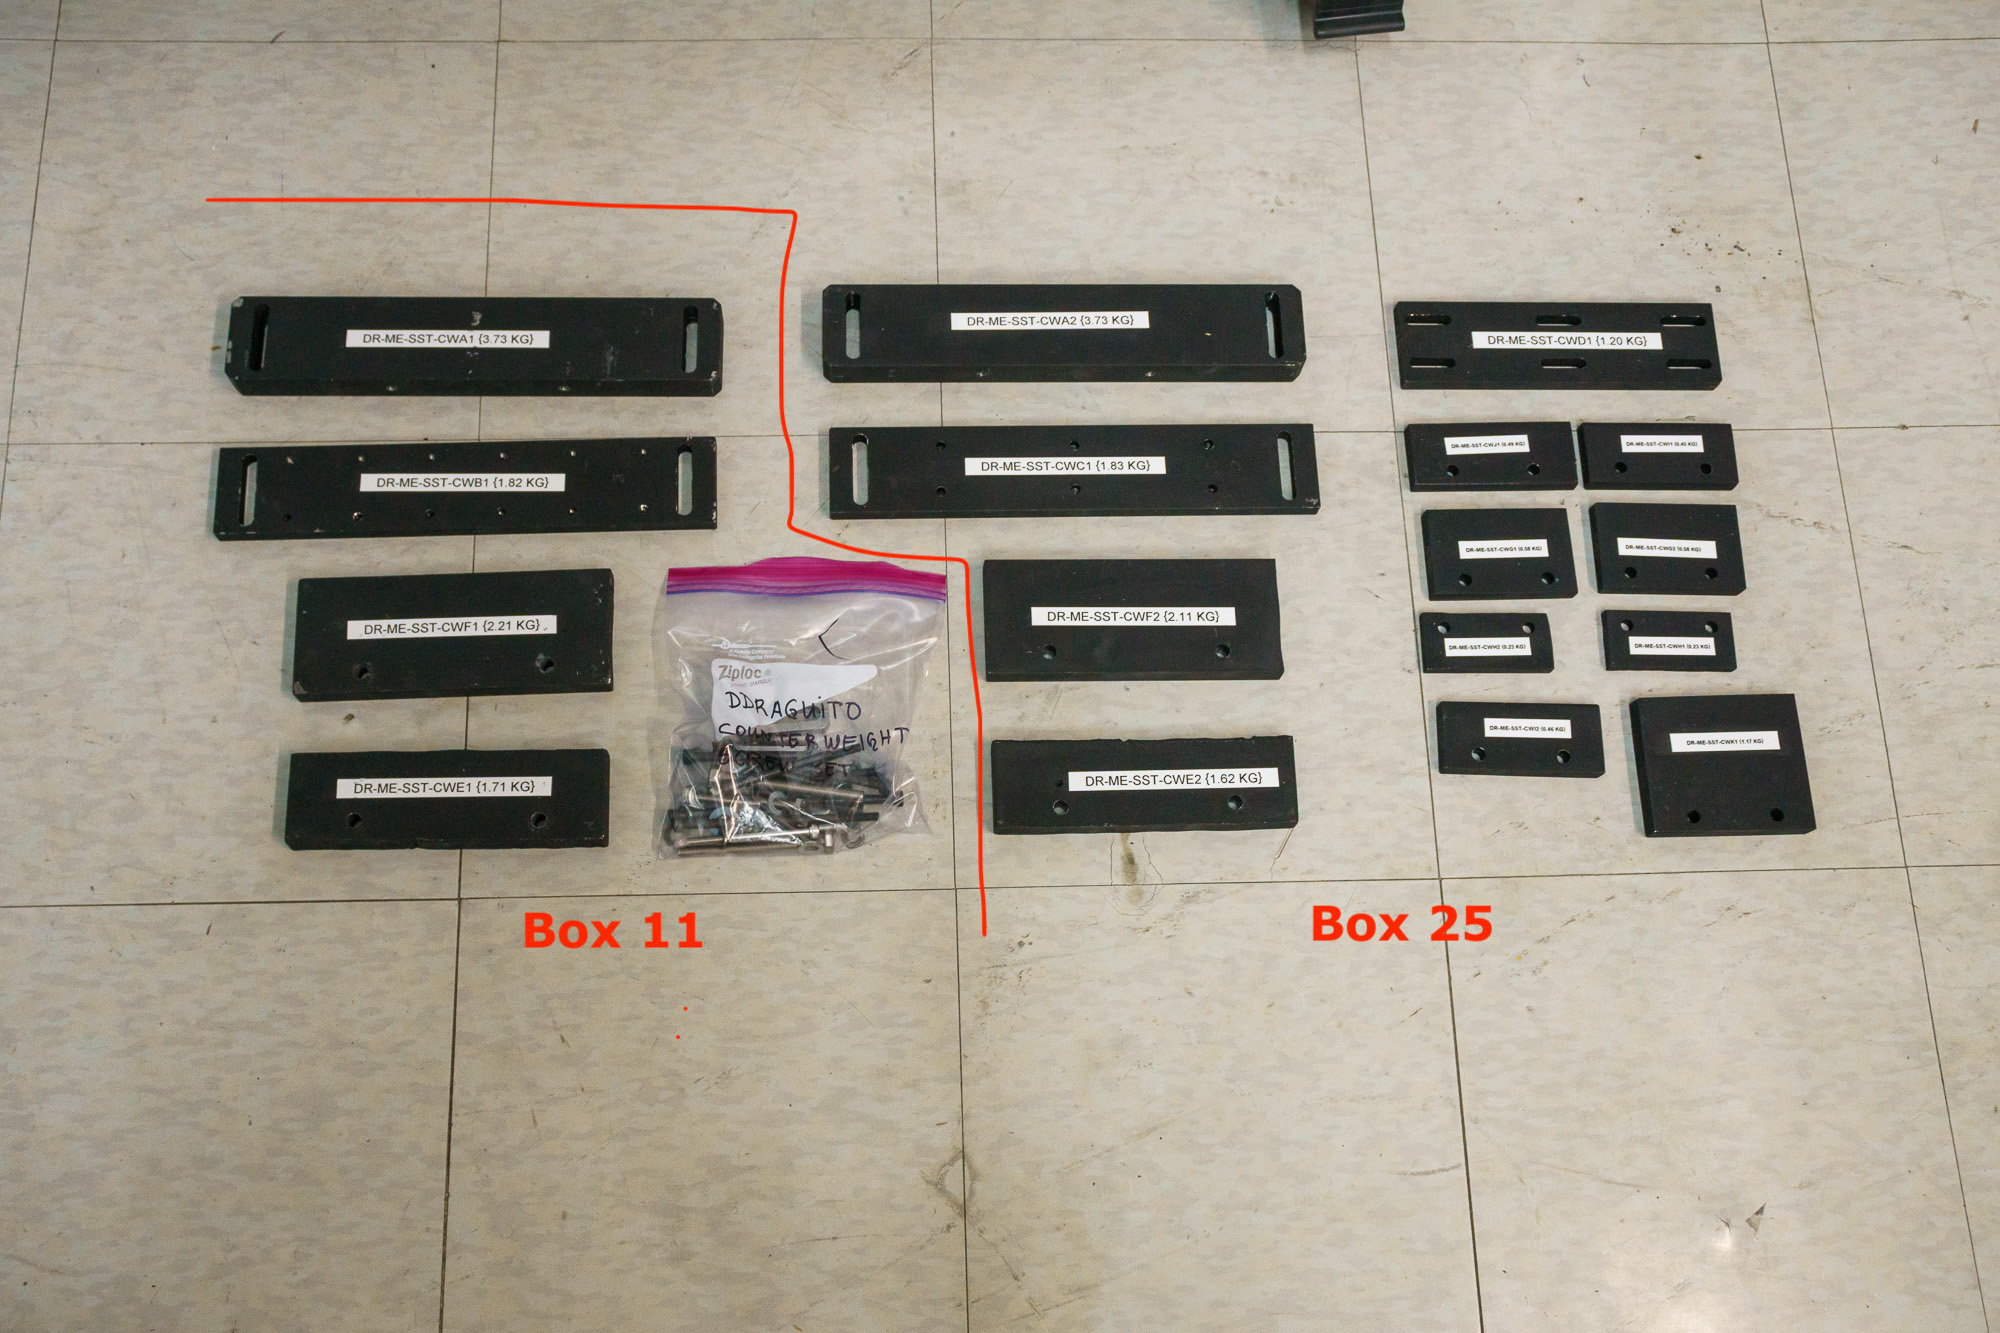
\includegraphics[width=0.80\linewidth]{figures/20201208T175508.jpg}
\end{center}
\caption{Box 11 contents (left).}
\label{figure:box-eleven-contents}
\end{figure}

\begin{figure}[bp]
\begin{center}
\includegraphics[width=0.40\linewidth]{figures/20201208T182441.jpg}
\includegraphics[width=0.40\linewidth]{figures/20201208T183054.jpg}\\[\smallskipamount]
\includegraphics[width=0.40\linewidth]{figures/20201208T183316.jpg}
\includegraphics[width=0.40\linewidth]{figures/20201208T183627.jpg}
\end{center}
\caption{Box 11 packing.}
\label{figure:box-eleven-packing}
\end{figure}

\subsection{Description}

Box 11 contains:

\begin{itemize}
    \item The counterweights DR-ME-SST-CWA1, DR-ME-SST-CWB1, DR-ME-SST-CWE1, and DR-ME-SST-CWF1. We're actually not sure if each of these is part 1 or 2 (e.g., DR-ME-SST-CWA1 or DR-ME-SST-CWA2), but since they are identical it makes no real difference. These counterweights are the nominal set for one set of legs.
    \item Assorted bolts to fasten the counterweights to the support structure.
\end{itemize}

The counterweights are wrapped in plastic. The bolts are packed in a plastic bag. The contents are placed in a cardboard box, lined on all sides with 25 mm polystyrene foam sheets. The space around the contents is filled with polystyrene packing peanuts. See Figure \ref{figure:box-eleven-contents} and \ref{figure:box-eleven-packing}.

Other counterweights are packed in Box 25.

Box 11 is $30 \times 30 \times 20$~cm ($L \times W \times H$) and has a weight of 11 kg.

\subsection{Unpacking Instructions}

There are no special unpacking instructions.

\subsection{Repacking Instructions}

There are no special repacking instructions.

%%%%%%%%%%%%%%%%%%%%%%%%%%%%%%%%%%%%%%%%%


\clearpage
\section{Boxes 12 to 17}

\begin{figure}[bp]
\begin{center}
\includegraphics[width=0.30\linewidth]{figures/20201207T135242.jpg}
\includegraphics[width=0.30\linewidth]{figures/20201207T135505.jpg}\\[\smallskipamount]
\includegraphics[width=0.30\linewidth]{figures/20201207T140609.jpg}
\includegraphics[width=0.30\linewidth]{figures/20201207T140836.jpg}\\[\smallskipamount]
\includegraphics[width=0.30\linewidth]{figures/20201207T140343.jpg}
\includegraphics[width=0.30\linewidth]{figures/20201207T140556.jpg}\\[\smallskipamount]
\includegraphics[width=0.30\linewidth]{figures/20201207T135859.jpg}
\includegraphics[width=0.30\linewidth]{figures/20201207T140137.jpg}\\[\smallskipamount]
\includegraphics[width=0.30\linewidth]{figures/20201207T135601.jpg}
\includegraphics[width=0.30\linewidth]{figures/20201207T135835.jpg}\\[\smallskipamount]
\includegraphics[width=0.30\linewidth]{figures/20201207T134559.jpg}
\includegraphics[width=0.30\linewidth]{figures/20201207T135049.jpg}
\end{center}
\caption{Boxes 12 (top) to 17 (bottom) and their contents.}
\label{figure:box-computers}
\end{figure}

\subsection{Description}

Boxes 12 to 17 each contain:

\begin{itemize}
    \item A HPE Proliant DL20 Gen 10 computer with rack-mounting hardware.
    \item A power cable.
    \item An Ethernet cable.
\end{itemize}

The precise contents are:

\begin{itemize}
    \item Box 12: DR-CO-CR-BLUE (with the PCIe card DR-CO-CR-BLUE-DPC installed), DR-CO-CR-BLUE-PWC, and DR-CO-CR-BLUE-ETHC.
    \item Box 13: DR-CO-CR-DETECTORS, DR-CO-CR-DETECTORS-PWC, and DR-CO-CR-DETECTORS-ETHC.
    \item Box 14: DR-CO-CR-CONTROL, DR-CO-CR-CONTROL-PWC, and DR-CO-CR-CONTROL-ETHC.
    \item Box 15: DR-CO-CR-SERVICES, DR-CO-CR-SERVICES-PWC, and DR-CO-CR-SERVICES-ETHC.
    \item Box 16: DR-CO-CR-SPARELINUX, DR-CO-CR-SPARELINUX-PWC, and DR-CO-CR-SPARELINUX-ETHC.
    \item Box 17: DR-CO-CR-SPAREWINDOWS, DR-CO-CR-SPAREWINDOWS-PWC, and DR-CO-CR-SPAREWINDOWS-ETHC.
\end{itemize}

See Figure~\ref{figure:box-computers}.

The boxes are the original boxes for the computers.

Each box is $77 \times 26 \times 57$~cm ($L \times W \times H$) and has a weight of 11 kg.

\subsection{Unpacking Instructions}

There are no special unpacking instructions.

\subsection{Repacking Instructions}

There are no special repacking instructions.

%%%%%%%%%%%%%%%%%%%%%%%%%%%%%%%%%%%%%%%%%

\clearpage
\section{Boxes 18 and 19}


\begin{figure}[bp]
\begin{center}
\includegraphics[width=0.40\linewidth]{figures/20201207T132215.jpg}
\includegraphics[width=0.40\linewidth]{figures/20201207T133020.jpg}\\[\smallskipamount]
\includegraphics[width=0.40\linewidth]{figures/20201207T132112.jpg}
\includegraphics[width=0.40\linewidth]{figures/20201207T132404.jpg}
\end{center}
\caption{Boxes 18 (top) and 19 (bottom) and their contents.}
\label{figure:box-switches}
\end{figure}

\subsection{Description}

Boxes 18 and 19 both contain:

\begin{itemize}
    \item A HPE OfficeConnect 1420 24G Ethernet Switch
\end{itemize}

The precise contents are:

\begin{itemize}
    \item Box 18: DR-CO-CR-SWITCH.
    \item Box 19: DR-CO-CR-SPARESWITCH.
\end{itemize}

See Figure~\ref{figure:box-switches}.

The boxes are the original boxes for the switches.

Each box is  $50 \times 27 \times 9$~cm ($L \times W \times H$) and has a weight of 3 kg.

\subsection{Unpacking Instructions}

There are no special unpacking instructions.

\subsection{Repacking Instructions}

There are no special repacking instructions.

%%%%%%%%%%%%%%%%%%%%%%%%%%%%%%%%%%%%%%%%%

\clearpage
\section{Boxes 20 to 22}

\begin{figure}[bp]
\begin{center}
\includegraphics[width=0.40\linewidth]{figures/20201207T133440.jpg}
\includegraphics[width=0.40\linewidth]{figures/20201207T133732.jpg}\\[\smallskipamount]
\includegraphics[width=0.40\linewidth]{figures/20201207T134111.jpg}
\includegraphics[width=0.40\linewidth]{figures/20201207T134343.jpg}\\[\smallskipamount]
\includegraphics[width=0.40\linewidth]{figures/20201207T133800.jpg}
\includegraphics[width=0.40\linewidth]{figures/20201207T134046.jpg}
\end{center}
\caption{Boxes 20 (top), 21 (middle), and 22 (bottom) and their contents.}
\label{figure:box-pdus}
\end{figure}

\subsection{Description}

Boxes 20 to 22 each contain:

\begin{itemize}
    \item A Dataprobe iBoot-PDU-C20 power distribution unit.
    \item An Ethernet cable.
\end{itemize}

The precise contents are:

\begin{itemize}
    \item Box 20: DR-CO-CR-PDU1 and DR-CO-CR-PDU1-ETHC.
    \item Box 21: DR-CO-CR-PDU2 and DR-CO-CR-PDU2-ETHC.
    \item Box 22: DR-CO-CR-PDUSPARE and DR-CO-CR-PDUSPARE-ETHC.
\end{itemize}

See Figure~\ref{figure:box-pdus}.

The boxes are the original boxes for the PDUs.

Each box is  $51 \times 29 \times 9$~cm ($L \times W \times H$) and has a weight of 3 kg.


\subsection{Unpacking Instructions}

There are no special unpacking instructions.

\subsection{Repacking Instructions}

There are no special repacking instructions.

%%%%%%%%%%%%%%%%%%%%%%%%%%%%%%%%%%%%%%%%%

\clearpage
\section{Box 23}

\begin{figure}[bp]
\begin{center}
\includegraphics[width=0.80\linewidth]{figures/20201207T141455.jpg}\\[\smallskipamount]
\end{center}
\caption{Box 23 contents.}
\label{figure:box-twenty-three-a}
\end{figure}

\begin{figure}[bp]
\begin{center}
\includegraphics[width=0.40\linewidth]{figures/20201207T142921.jpg}
\includegraphics[width=0.40\linewidth]{figures/20201207T143100.jpg}
\end{center}
\caption{Box 23 packing.}
\label{figure:box-twenty-three-b}
\end{figure}

\subsection{Description}

Box 23 contains:

\begin{itemize}
    \item The Mac mini computer DR-CO-CR-ACCESS.
    \item The Ethernet cable DR-CO-CR-ACCESS-ETHC.
    \item The power cables DR-CO-CR-ACCESS-PWC and DR-CO-CR-ACCESS-EPWC.
    \item The VGA adapter DR-CO-CR-ACCESS-VAD.
\end{itemize}

The Mac mini is wrapped in bubble wrap. The contents are then packed in a cardboard box lined on all sides with 25~mm polystyrene foam sheets. See Figure~\ref{figure:box-twenty-three-a} and \ref{figure:box-twenty-three-b}.

Box 23 is  $30 \times 30 \times 20$~cm ($L \times W \times H$) and has a weight of 2 kg.

\subsection{Unpacking Instructions}

There are no special unpacking instructions.

\subsection{Repacking Instructions}

There are no special repacking instructions.

%%%%%%%%%%%%%%%%%%%%%%%%%%%%%%%%%%%%%%%%%

\clearpage
\section{Box 24}

\begin{figure}[bp]
\begin{center}
\includegraphics[width=0.80\linewidth]{figures/20201208T180354.jpg}
\end{center}
\caption{Box 24 contents.}
\label{figure:box-twenty-four-a}
\end{figure}

\begin{figure}[bp]
\begin{center}
\includegraphics[width=0.40\linewidth]{figures/20201208T183054.jpg}
\includegraphics[width=0.40\linewidth]{figures/20201208T183316.jpg}\\[\smallskipamount]
\includegraphics[width=0.40\linewidth]{figures/20201208T183414.jpg}
\includegraphics[width=0.40\linewidth]{figures/20201208T183627.jpg}
\end{center}
\caption{Box 24 packing.}
\label{figure:box-twenty-four-b}
\end{figure}

\subsection{Description}

Box 24 contains:

\begin{itemize}
    \item The cable-handling hardware DR-ME-SST-CWS1, DR-ME-SST-CWS2, DR-ME-SST-CWSP, DR-ME-SST-CWSS, DR-ME-SST-CG1, and 
DR-ME-SST-CG2.
\item Twelve M8$\times$40 bolts (to fasten DR-ME-SST-CWSP/CWSS to DR-ME-SST-FP1).
\item Two M5$\times$15 bolts (to fasten DR-ME-SST-CG2 to DR-ME-SST-FP1).
\end{itemize}

The pieces DR-ME-SST-CWS1, DR-ME-SST-CWS2, DR-ME-SST-CWSP, and DR-ME-SST-CG are shipped assembled. The pieces are wrapped in plastic. The bolts are packed in plastic bags. The contents are then placed in a cardboard box, lined on all sides with 25 mm polystyrene foam sheets. The space around the contents is then filled with polystyrene pieces and packing peanuts. See Figure \ref{figure:box-twenty-four-a} and \ref{figure:box-twenty-four-b}

Box 24 is  $45 \times 45 \times 25$~cm ($L \times W \times H$) and has a weight of 8 kg.

\subsection{Unpacking Instructions}

There are no special unpacking instructions.

\subsection{Repacking Instructions}

There are no special repacking instructions.

%%%%%%%%%%%%%%%%%%%%%%%%%%%%%%%%%%%%%%%%%

\clearpage
\section{Box 25}

\begin{figure}[bp]
\begin{center}
\includegraphics[width=0.80\linewidth]{figures/20201208T175508.jpg}
\end{center}
\caption{Box 25 contents (right).}
\label{figure:box-twenty-five-contents}
\end{figure}

\begin{figure}[bp]
\begin{center}
\includegraphics[width=0.40\linewidth]{figures/20201208T182456.jpg}
\includegraphics[width=0.40\linewidth]{figures/20201208T184035.jpg}\\[\smallskipamount]
\includegraphics[width=0.40\linewidth]{figures/20201208T184111.jpg}
\includegraphics[width=0.40\linewidth]{figures/20201208T184229.jpg}
\end{center}
\caption{Box 25 packing.}
\label{figure:box-twenty-five-packing}
\end{figure}

\subsection{Description}

Box 25 contains:

\begin{itemize}
    \item The counterweights DR-ME-SST-CWA2, DR-ME-SST-CWC1, DR-ME-SST-CWE2, and DR-ME-SST-CWF2. We're actually not sure if each of these is part 1 or 2 (e.g., DR-ME-SST-CWA1 or DR-ME-SST-CWA2), but since they are identical it makes no real difference. These counterweights are the nominal set for one set of legs.
    \item The additional counterweights DR-ME-SST-CWD1, DR-ME-SST-CWG1, DR-ME-SST-CWG2, DR-ME-SST-CWH1, DR-ME-SST-CWH2, DR-ME-SST-CWI1, DR-ME-SST-CWI2, DR-ME-SST-CWJ1, and DR-ME-SST-CWK1. These are smaller weights for fine balance adjustment.
\end{itemize}

The counterweights are wrapped in plastic. The contents are placed in a cardboard box, lined on all sides with 25 mm polystyrene foam sheets. The space around the contents is filled with polystyrene packing peanuts. See Figure \ref{figure:box-twenty-five-contents} and \ref{figure:box-twenty-five-packing}.

Box 25 is $30 \times 30 \times 20$~cm ($L \times W \times H$) and has a weight of 15 kg.

\subsection{Unpacking Instructions}

There are no special unpacking instructions.

\subsection{Repacking Instructions}

There are no special repacking instructions.

%%%%%%%%%%%%%%%%%%%%%%%%%%%%%%%%%%%%%%%%%

\clearpage
\section{Box 26}

\begin{figure}[bp]
\begin{center}
\includegraphics[width=0.80\linewidth]{figures/20201208T173642.jpg}\\[\smallskipamount]
\includegraphics[width=0.80\linewidth]{figures/20201208T173648.jpg}
\end{center}
\caption{Box 26 contents.}
\label{figure:box-twenty-six-contents}
\end{figure}

\begin{figure}[bp]
\begin{center}
\includegraphics[width=0.40\linewidth]{figures/20201208T174135.jpg}\\[\smallskipamount]
\includegraphics[width=0.40\linewidth]{figures/20201208T174256.jpg}\\[\smallskipamount]
\includegraphics[width=0.40\linewidth]{figures/20201208T174457.jpg}
\end{center}
\caption{Box 26 packing.}
\label{figure:box-twenty-six-packing}
\end{figure}

\subsection{Description}

Box 26 contains:

\begin{itemize}
    \item The blue detector and filter wheel optomechanics: DR-ME-SST-RP3, 
DR-ME-OMBD-ADR,
DR-ME-OMBD-FL(1-2),
DR-ME-OMBD-LT,
DR-ME-OMBD-AB(1-3),
DR-ME-OMBD-OLNA(1-3),
DR-ME-OMBD-OLNB(1-3),
DR-ME-OMBD-ILN(1-3), and
DR-ME-OMBD-FC
\item The blue detector outer light trap: DR-ME-OMBD-OLTC(A-B) and DR-ME-OMBD-OLTR(1-3).
\item Twenty five M6$\times$20 screws to fasten DR-ME-SST-RP3 to the main structure.
\item Eight M3 screws to fasten DR-ME-OMBD-OLTC(A-B) to DR-ME-OMBD-ADR.
\item The fasteners to secure the filters in the filter wheel.
\end{itemize}

The fasteners are placed in plastic bags. The contents are wrapped in plastic. The contents are placed in a cardboard box, lined on all sides with 25 mm polystyrene foam sheets. The space around the contents is filled with polystyrene packing peanuts. See Figure \ref{figure:box-twenty-six-contents} and \ref{figure:box-twenty-six-packing}.

Box 26 is  $60 \times 60 \times 30$~cm ($L \times W \times H$) and has a weight of 14 kg.

\subsection{Unpacking Instructions}

There are no special unpacking instructions.

\subsection{Repacking Instructions}

There are no special repacking instructions.

%%%%%%%%%%%%%%%%%%%%%%%%%%%%%%%%%%%%%%%%%

\clearpage
\section{Box 27}

\begin{figure}[bp]
\begin{center}
\includegraphics[width=0.80\linewidth]{figures/20210106T114250.jpg}
\end{center}
\caption{Box 27 contents.}
\label{figure:box-twenty-seven-contents}
\end{figure}

\begin{figure}[bp]
\begin{center}
\includegraphics[width=0.40\linewidth]{figures/20201209T080350.jpg}
\includegraphics[width=0.40\linewidth]{figures/20210106T114250.jpg}\\[\smallskipamount]
\includegraphics[width=0.40\linewidth]{figures/20210106T114314.jpg}
\includegraphics[width=0.40\linewidth]{figures/20201209T080416.jpg}\\[\smallskipamount]
\includegraphics[width=0.40\linewidth]{figures/20201209T080424.jpg}
\includegraphics[width=0.40\linewidth]{figures/20201209T114456.jpg}
\end{center}
\caption{Box 27 packing.}
\label{figure:box-twenty-seven-packing}
\end{figure}

\subsection{Description}

Box 27 contains:

\begin{itemize}
    \item The spherical test mirror DR-OP-STM and its optomechanical assembly DR-TE-OMSTM.
    \item Screws to fasten OMSTM to the instrument.
\end{itemize}

The fasteners are placed in a plastic bag. The contents are wrapped in plastic. The contents are placed in a cardboard box, with layers of bubble wrap below and above and surrounded by specially cut sheets of 25 mm polystyrene foam. See Figure \ref{figure:box-twenty-seven-contents} and \ref{figure:box-twenty-seven-contents}.

Box 27 is  $60 \times 50 \times 50$~cm ($L \times W \times H$) and has a weight of 20 kg.

\subsection{Unpacking Instructions}

There are no special unpacking instructions.

\subsection{Repacking Instructions}

\begin{enumerate}
    \item Wrap the OMSTM in plastic.
    \item Place bubble-wrap at the bottom of the box.
    \item Place an uncut sheet of polystyrene foam above the bubble wrap.
    \item Place the OMSTM and the cut sheets of polystyrene in the box.
    \item Tape the fasteners to a sheet.
    \item Surround the OMSTM with bubble wrap.
    \item Place an uncut sheet of polystyrene foam above the OMSTM.
    \item Place layers of bubble wrap above the sheet.
    \item Add dessicant.    
    \item Close the box.
\end{enumerate}

%%%%%%%%%%%%%%%%%%%%%%%%%%%%%%%%%%%%%%%%%

\clearpage
\section{Box 28}

\begin{figure}[bp]
\begin{center}
\includegraphics[width=0.80\linewidth]{figures/20201209T140203.jpg}
\includegraphics[width=0.80\linewidth]{figures/20210108T140347.jpg}
\end{center}
\caption{Box 28 contents.}
\label{figure:box-twenty-eight-contents}
\end{figure}

\begin{figure}[bp]
\begin{center}
\includegraphics[width=0.40\linewidth]{figures/20201209T140919.jpg}
\includegraphics[width=0.40\linewidth]{figures/20201209T142113.jpg}\\[\smallskipamount]
\includegraphics[width=0.40\linewidth]{figures/20201209T142229.jpg}
\includegraphics[width=0.40\linewidth]{figures/20201209T142335.jpg}\\[\smallskipamount]
\includegraphics[width=0.40\linewidth]{figures/20201209T142403.jpg}
\end{center}
\caption{Box 28 packing.}
\label{figure:box-twenty-eight-packing}
\end{figure}

\subsection{Description}

Box 28 contains the following spare parts:

\begin{itemize}
    \item Spare filter wheel.
    \item Spare shutter.
    \item Spare Icron Ranger 2324 USB extender LEX and REX.
    \item Spare fan, thermostats (NC and NO), heater, 12 VDC power supply, and 24 VDC power supply for the close electronics.
    \item Spare 1-wire adapter, 1-wire MS-TH sensor, and 1-wire EDS OW-ENV-THPL sensor.
    \item Spare $5g$ and $10g$ impact sensors. Spare temperature sensors.
\end{itemize}

The contents are wrapped in plastic and bubble wrap. The contents are placed in a cardboard box, lined on all sides with 25 mm polystyrene foam sheets. The space around the contents is filled with polystyrene packing peanuts. See Figure \ref{figure:box-twenty-eight-contents} and \ref{figure:box-twenty-eight-packing}.

Box 28 is  $45 \times 45 \times 25$~cm ($L \times W \times H$) and has a weight of 7 kg.

\subsection{Unpacking Instructions}

There are no special unpacking instructions.

\subsection{Repacking Instructions}

There are no special repacking instructions.

%%%%%%%%%%%%%%%%%%%%%%%%%%%%%%%%%%%%%%%%%

\clearpage
\section{Box 29}

\begin{figure}[bp]
\begin{center}
\includegraphics[width=0.60\linewidth]{figures/20201209T125026.jpg}
\includegraphics[width=0.60\linewidth]{figures/20201209T135331.jpg}
\includegraphics[width=0.60\linewidth]{figures/20201209T143011.jpg}
\end{center}
\caption{Box 29 contents.}
\label{figure:box-twenty-nine-contents}
\end{figure}

\begin{figure}[bp]
\begin{center}
\includegraphics[width=0.40\linewidth]{figures/20201209T134047.jpg}
\includegraphics[width=0.40\linewidth]{figures/20201209T135706.jpg}\\[\smallskipamount]
\includegraphics[width=0.40\linewidth]{figures/20201209T135753.jpg}
\includegraphics[width=0.40\linewidth]{figures/20201209T135846.jpg}\\[\smallskipamount]
\includegraphics[width=0.40\linewidth]{figures/20201209T140034.jpg}
\includegraphics[width=0.40\linewidth]{figures/20201209T140048.jpg}\\
\end{center}
\caption{Box 29 packing.}
\label{figure:box-twenty-nine-packing}
\end{figure}

\subsection{Description}

Box 29 contains the following tools:

\begin{itemize}
    \item The refill hose DR-CO-CR-DSC-RH.
    \item The refill hose wrench DR-CO-CR-DSC-RHWR.
    \item The torquemeter wrench DR-CO-CR-DSC-TM for tightening the hose connectors to the correct torque.
    \item The vacuum adapters DR-CO-DH-VPA and DR-CO-DH-VHA25, sealed together with silicone sealer.
    \item The vacuum port power supply DR-CO-DH-VPPS.
    \item Grease and hex keys for Roxtec cable pass.
    \item O-rings for cryogen hoses (in the torquemeter box)
\end{itemize}

The contents are wrapped in bubble wrap and plastic.  The contents are placed in a cardboard box, lined on all sides with 25 mm polystyrene foam sheets. The space around the contents is filled with polystyrene packing peanuts. See Figure \ref{figure:box-twenty-nine-contents} and \ref{figure:box-twenty-nine-packing}.

Box 29 is $45 \times 45 \times 25$~cm ($L \times W \times H$) and has a weight of 5 kg.

\subsection{Unpacking Instructions}

There are no special unpacking instructions.

\subsection{Repacking Instructions}

There are no special repacking instructions.

%%%%%%%%%%%%%%%%%%%%%%%%%%%%%%%%%%%%%%%%%

\clearpage
\section{Box 30}

\begin{figure}[bp]
\begin{center}
\includegraphics[width=0.80\linewidth]{figures/20201209T111843.jpg}\\[\smallskipamount]
\includegraphics[width=0.80\linewidth]{figures/20201210T105443.jpg}
\end{center}
\caption{Box 30 contents.}
\label{figure:box-thirty-contents}
\end{figure}

\begin{figure}[bp]
\begin{center}
\includegraphics[width=0.40\linewidth]{figures/20201209T112420.jpg}
\includegraphics[width=0.40\linewidth]{figures/20201209T114825.jpg}\\[\smallskipamount]
\includegraphics[width=0.40\linewidth]{figures/20201209T114927.jpg}
\includegraphics[width=0.40\linewidth]{figures/20201209T114939.jpg}\\[\smallskipamount]
\includegraphics[width=0.40\linewidth]{figures/20201209T115134.jpg}
\end{center}
\caption{Box 30 packing.}
\label{figure:box-thirty-packing}
\end{figure}

\subsection{Description}

Box 30 contains materials for mounting the instrument:

\begin{itemize}
    \item The alignment pin DR-ME-MH-PIN(1-4).
    \item The slings DR-ME-MH-SL(1-4)
    \item The turnbuckles DR-ME-MH-TB(1-4)
    \item The connecting links DR-ME-MH-CL(1-8)
    \item Three M12$\times$25 screws to fix the centering ring DR-ME-SST-CR to the derotator.
    \item Twenty one M12$\times$50 screws and washers to fix the plate DR-ME-SST-FP1 to the derotator.
\end{itemize}

The contents are wrapped in bubble wrap and plastic.  The contents are placed in a cardboard box, lined on all sides with 25 mm polystyrene foam sheets. The space around the contents is filled with polystyrene packing peanuts. See Figure \ref{figure:box-thirty-contents} and \ref{figure:box-thirty-packing}.

Box 30 is $45 \times 45 \times 25$~cm ($L \times W \times H$) and has a weight of 7 kg.

\subsection{Unpacking Instructions}

There are no special unpacking instructions.

\subsection{Repacking Instructions}

There are no special repacking instructions.



\end{document}
